\documentclass{tudelft-report}

%% additional packages
\usepackage{pdfpages}

\usepackage{afterpage}
\newcommand\blankpage{%
    \null
    \thispagestyle{empty}%
    \addtocounter{page}{-1}%
    \newpage}

\usepackage{lipsum}
\usepackage{multirow}
\usepackage{multicol}
\usepackage{xcolor,colortbl}
\usepackage{tabularx}
\usepackage{listings}
\usepackage{appendix}

\definecolor{lightgrey}{rgb}{0.9,0.9,0.9}
\definecolor{neonyellow}{rgb}{1,1,0}
\definecolor{lightblue}{rgb}{0,0.5,1}
\definecolor{orange}{rgb}{1,0.5,0} 
\definecolor{pink}{rgb}{1,0,0.5}
\definecolor{vectorGreen}{rgb}{0,1,0}

\definecolor{dotblue}{rgb}{0,0.68,0.93}

\newcolumntype{a}{>{\columncolor{Gray}}c}
\newcolumntype{b}{>{\columncolor{white}}c}
\newcommand\tab[1][1cm]{\hspace*{#1}}

\usepackage{hyphenat}
\usepackage[framemethod=tikz]{mdframed}
\usepackage[most]{tcolorbox}
\usepackage{lipsum}
\usepackage[justification=centering]{caption}
\usepackage{ragged2e}
\usepackage[export]{adjustbox}
\usepackage{graphicx,nicefrac}
% \usepackage{subcaption}
\usepackage{can  cel}
% \usepackage[table]{xcolor}


\newtcolorbox{definitioni}{
  breakable,
  fonttitle=\bfseries,
  title={Info}
}

\newcommand*{\bluebullet}{\textcolor{dotblue}{\textbullet} \medskip}

% mathematica
\usepackage{amsmath, amsthm, amssymb, graphics, setspace}
\DeclareMathOperator*{\argmin}{argmin}

\newcommand{\mathsym}[1]{{}}
\newcommand{\unicode}[1]{{}}


% ------------------------------------------------------------------------
\let\cleardoublepage\clearpage
\usepackage{array, booktabs}
\newcolumntype{L}[1]{>{\raggedright\let\newline\\\arraybackslash}m{#1}}
\usepackage{longtable}
\newcolumntype{C}[1]{>{\centering\arraybackslash}p{#1}}
\usepackage{parskip}% http://ctan.org/pkg/parskip

% commands to stop hyphenating in the entire document
\tolerance=1
\emergencystretch=\maxdimen
\hyphenpenalty=10000
\hbadness=10000


\usepackage{algorithm2e}
\RestyleAlgo{ruled}


\usepackage[
backend=biber,
style=numeric,
citestyle=numeric,
sorting=none
]{biblatex}


\addbibresource{report.bib} %Imports bibliography file

\usepackage{minted}
\usepackage{emoji}

%--------------------------------------------------------------------------
\usepackage[export]{adjustbox}
\usepackage{float}
\usepackage{wrapfig}
% \usepackage[utf8x]{inputenc}
\usepackage[colorinlistoftodos]{todonotes}
% \usepackage{minted}
% \usemintedstyle{vs}
\usepackage{subfigure}
% \usepackage[demo]{graphicx}


\usepackage{pdflscape}
\usepackage{rotating}

\usepackage{makecell}
% \usepackage{graphicx}
\renewcommand\theadalign{bc}
\renewcommand\theadfont{\bfseries}
\renewcommand\theadgape{\Gape[2pt]}
\renewcommand\cellgape{\Gape[2pt]}
% \newcommand*{\thead}[1]{%
% \multicolumn{1}{c}{\bfseries\begin{tabular}{@{}c@{}}#1\end{tabular}}}

\begin{document}
%% Use Roman numerals for the page numbers of the title pages and table of
%% contents.


\frontmatter



\newcommand{\uproman}[1]{\uppercase\expandafter{\romannumeral#1}}

\begin{titlepage}

% Logo
% \tikz[remember picture,overlay] \node[opacity=0.3,inner sep=0pt] at (current page.center){
% % 
\includegraphics[width=\paperwidth,height=\paperheight]{images/IMS.pdf}
% };

\includegraphics[width=0.5\textwidth]{images/zhaw_logo.png}


\vskip 1.0cm
%\textbf{0.117\textwidth}
\begin{minipage}[b]{0.14\textwidth}
	\hskip 0.05cm
\end{minipage}
%0.91\textwidth
\begin{minipage}[b]{0.84\textwidth}
\begin{tiny}.\end{tiny}\vskip 2.8cm
	{\huge
	
%-----------------------------------------------------------------------------
% Projekttitel
%------------------------------------------------------------------------------

	\textbf{\underline{MSE Master's Thesis}}\\
	
	% Projekt Titel
	\begin{minipage}[b]{0.9\textwidth}
% 		Intrinsically Motivated \\ Voxel-based Scene Understanding \\
% 		Exploiting Voxels and Octrees in\\Active Vision for Scene Understanding \\
% 		Octree Exploration of Voxelized Scenes with Active Vision for Scene Understanding \\
% 		Voxelized Octree Exploration of 3D Scenes with Entropy-aware Active Vision for Scene Understanding \\
		Entropy-Aware Active Vision through Voxelized Octree Exploration of 3D Scenes \\
	\end{minipage}

	\begin{minipage}[b]{0.1\textwidth}
	\end{minipage}
	\vskip 0.5cm}

%------------------------------------------------------------------------------
% Autoren
%------------------------------------------------------------------------------
	

	\begin{minipage}[b]{0.27\textwidth}
% 	\vskip 0.5cm
	\hrule\vskip 0.5cm
		\textbf{Autor}\\
	\end{minipage}
	\begin{minipage}[b]{0.03\textwidth}
	\hskip 0.5cm
	\end{minipage}
	\begin{minipage}[b]{0.7\textwidth}
	\hrule\vskip 0.5cm
		Juan F. Ribera Laszkowski \\
	\end{minipage}

%------------------------------------------------------------------------------
% Hauptbetreuung
%------------------------------------------------------------------------------
	
	\begin{minipage}[b]{0.27\textwidth}
	\hrule\vskip 0.5cm
		\textbf{Betreuung}\\
	\end{minipage}
	\begin{minipage}[b]{0.03\textwidth}
	\hskip 0.5cm
	\end{minipage}
	\begin{minipage}[b]{0.7\textwidth}
	\hrule\vskip 0.5cm
		Prof. Dr. Thilo Stadelmann \\
	\end{minipage}

%------------------------------------------------------------------------------
% Nebenbetreuung
%------------------------------------------------------------------------------
	
	\begin{minipage}[b]{0.27\textwidth}
	\hrule\vskip 0.5cm
		\textbf{Nebenbetreuung}\\
	\end{minipage}
	\begin{minipage}[b]{0.03\textwidth}
	\hskip 0.5cm
	\end{minipage}
	\begin{minipage}[b]{0.7\textwidth}
	\hrule\vskip 0.5cm
		Dr. Giovanni Toffetti Carughi \\
	\end{minipage}
	
%------------------------------------------------------------------------------
% Industriepartner
%------------------------------------------------------------------------------
	
	\begin{minipage}[b]{0.27\textwidth}
	\hrule\vskip 0.5cm
		\textbf{Industriepartner}\\
	\end{minipage}
	\begin{minipage}[b]{0.03\textwidth}
	\hskip 0.5cm
	\end{minipage}
	\begin{minipage}[b]{0.7\textwidth}
	\hrule\vskip 0.5cm
		Sutter Landtechnik GmbH \\
	\end{minipage}

%------------------------------------------------------------------------------	
% Datum
%------------------------------------------------------------------------------
	
	\begin{minipage}[b]{0.27\textwidth}
	\hrule\vskip 0.5cm
		\textbf{Datum}
	\end{minipage}
	\begin{minipage}[b]{0.03\textwidth}
	\hskip 0.5cm
	\end{minipage}
	\begin{minipage}[b]{0.7\textwidth}
	\hrule\vskip 0.5cm
		30.10.2021
	\end{minipage}
\end{minipage}
\vskip 0.5cm


\end{titlepage}

\afterpage{\blankpage}

% \input{content/preface}
\setcounter{page}{1}
% \chapter*{\LARGE Erklärung betreffend das selbstständige Verfassen \\
% einer Masterarbeit an der School of Engineering}
\chapter*{\LARGE Declaration concerning the independent writing \\
of a master thesis at the School of Engineering}
%\setheader{Selbstaendigkeitserklärung}
% Mit der Abgabe dieser Masterarbeit versichert der Studierende, dass er die Arbeit selbstständig und ohne fremde Hilfe verfasst hat. (Bei Gruppenarbeiten gelten die Leistungen der übrigen Gruppenmitglieder nicht als fremde Hilfe) \\ \\
% Der unterzeichnende Studierende erklärt, dass alle zitierten Quellen (auch Internetseiten) im Text oder Anhang korrekt nachgewiesen sind, d.h. dass die Masterarbeit keine Plagiate enthält, also keine Teile, die teilweise oder vollständig aus einem fremden Text oder einer fremden Arbeit unter Vorgabe der eigenen Urheberschaft bzw. ohne Quellenangabe übernommen worden sind. \\ \\
% Bei Verfehlungen aller Art treten die Paragraphen 39 und 40 (Unredlichkeit und Verfahren bei Unredlichkeit) der ZHAW Prüfungsordnung sowie die Bestimmungen der Disziplinarmassnahmen der Hochschulordnung in Kraft. \\
By submitting this Master's thesis, the student assures that he/she has written the thesis independently and without outside help. (In the case of group work, the performance of the other group members does not count as outside help). \\ \\
The undersigned student declares that all cited sources (including Internet pages) in the text or appendix are correctly accounted for, i.e. that the master's thesis does not contain any plagiarism, i.e. no parts that have been taken over in part or in full from another's text or work under pretence of one's own authorship or without citation of the source. \\ \\
In the event of misconduct of any kind, Sections 39 and 40 (Dishonesty and Procedure in the Event of Dishonesty) of the ZHAW Examination Regulations and the provisions of the Disciplinary Measures of the University Regulations shall come into force. \\
\vspace{50pt} \\
\begin{flushright}
	\noindent \rule{7.0cm}{0.4pt} \par
	\scriptsize{Date, Signature} \hspace{3cm} \textbf{\scriptsize{Juan Ribera}}
\end{flushright}
\chapter*{Abstract}
\setheader{Abstract}
%  TAKEN FROM MY GOOGLE DOCS

The large and still increasing popularity of deep learning, along with the growing availability of 3D labeled datasets has been setting the stage to the continuous development of new algorithms in scene understanding and exploration of unknown environments. However, these works continue to build modular and hierarchical architectures, engineer complex features in the pre-processing stage and lack reproducibility.

Current methods use either LiDAR data, RGBD data or point clouds to reconstruct top-down 2D maps for exploration in traditional benchmarks or simplistic or limited 3D environments. These methods are computationally and memory-wise expensive and depend heavily on the training data. We tackle the problem of exploration in an unknown environment by exploiting octrees for efficient navigation of 3D scenes, where we also define the uninformativeness in an unknown environment through voxelized objects and semantic entropy.

The key contribution of this thesis is a novel voxel- and octree-based exploration method that builds upon model-free reinforcement learning to enable visual-agnostic exploration of environments and objects, while also taking into account the inconsistencies in the temporal class density present in the environment. 
We demonstrate that our method outperforms Unity implementations of previous classical and geometric approaches and improves upon current state-of-the-art exploration methods that are motivated by coverage maximization and semantic curiosity.
% We demonstrate that our method outperforms previous classical and geometric approaches and improves upon current state-of-the-art exploration methods that are motivated by coverage maximization and semantic curiosity.

Moreover, by using voxels for exhaustive exploration of objects and grid sensors with panoramic coverage, our method bridges the gap between synthetic data and real data for the exploration of 3D environments, where the data distribution plays a key role in the performance of transfer learning techniques, enabling the agent to adapt to new environments without changes in its behavior.

Finally, with an ever increasing amount of algorithms, traditional benchmarks become uninformative and allow room for the creation of newer ones capable of testing more sophisticated challenges, representative of the real world. Motivated by recent works in the Unity 3D engine, we contribute three 3D environments that can be extended for the creation of new benchmarks, testing of new exploration methods and for a variety of other tasks such as synthetic data generation, autonomous driving, exploration, navigation, point-to-goal tasks, etc. The code base for our method can be found at \url{https://github.com/Ademord/ma-unity}. All Unity 3D Assets are protected by copyright.


% Computer vision has been a field of study since the 1960s, and over the past few years a lot of challenges, such as 2D object recognition are now considered solved problems. Nevertheless, default uncertainty in all environments is the basis of all vision problems, such as detection and recognition.
% The goal of this work is to analyze diverse exploration policies using reinforcement learning, and find an applicable solution for unknown 3D environments. 
% This work will contribute to the computer vision challenges encountered by the project "Melkroboter" project at the ZHAW.
% \chapter*{Summary}
\setheader{Summary}
\lipsum[1-2]





\chapter*{Preface}
\setheader{Preface}
% \lipsum[1-3]
I would like to give special thanks to my supervisors Thilo Stadelmann and Giovanni Toffeti for their continuous support during this Thesis work, for their great feedback and constructive discussions. I am very grateful to have been given the opportunity to explore and contribute to the ongoing research topics of reinforcement learning, computer vision and cloud robotics.  


\tableofcontents

%% Use Arabic numerals for the page numbers of the chapters.
\mainmatter

\chapter{Introduction}\label{chap:introduction}
% \section{Introduction}
% 2 pages
%   \begin{figure}[!ht]
%         \centering
%         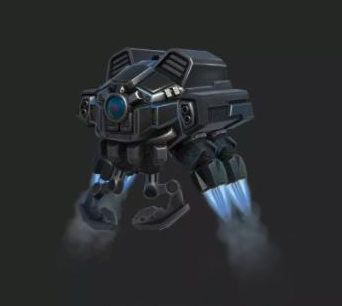
\includegraphics[width=0.5\textwidth]{images/drone.png}
%         \caption{3D Model of our Explorer Drone, from the Unity Asset Store \cite{unity2021}.}
%         \label{fig:cow_fmc}
%     \end{figure}
    
    
% \begin{figure}[!ht]
%     \centering
%     % \subfigure{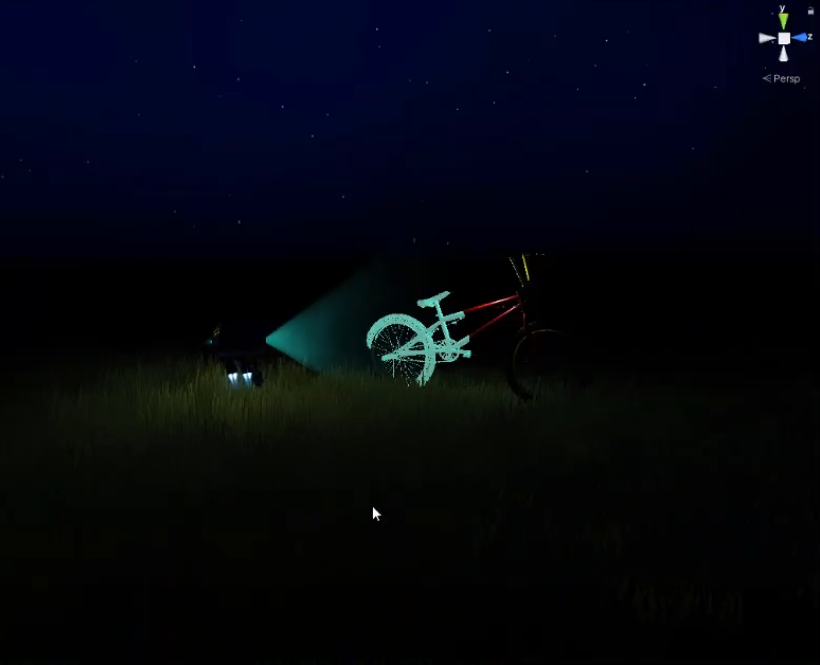
\includegraphics[width=0.315\textwidth]{images/unity-frontpage-drone2.png}} 
%     \subfigure{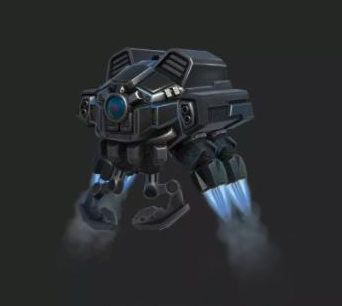
\includegraphics[width=0.287\textwidth]{images/drone.png}} 
%     \subfigure{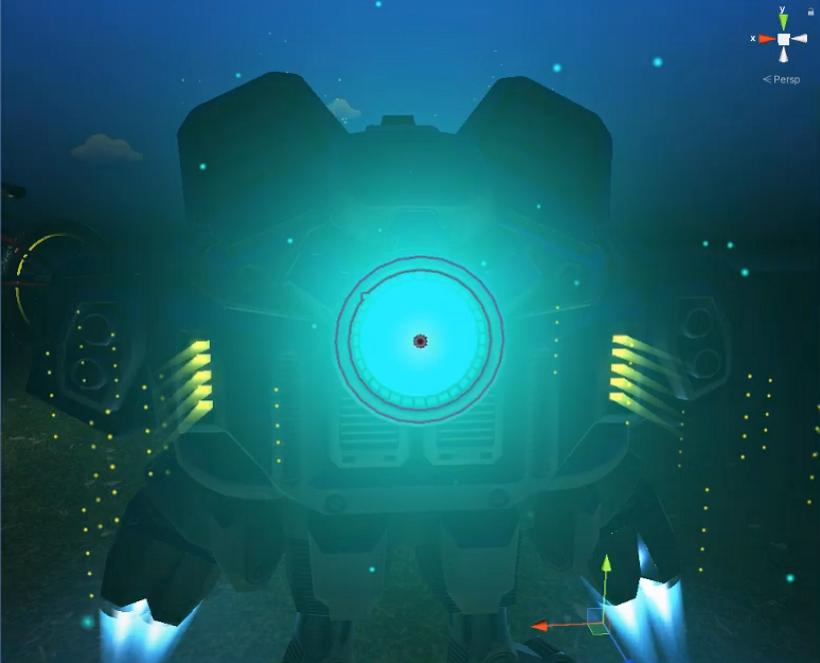
\includegraphics[width=0.317\textwidth]{images/unity-frontpage-drone1.png}} 
%     \subfigure{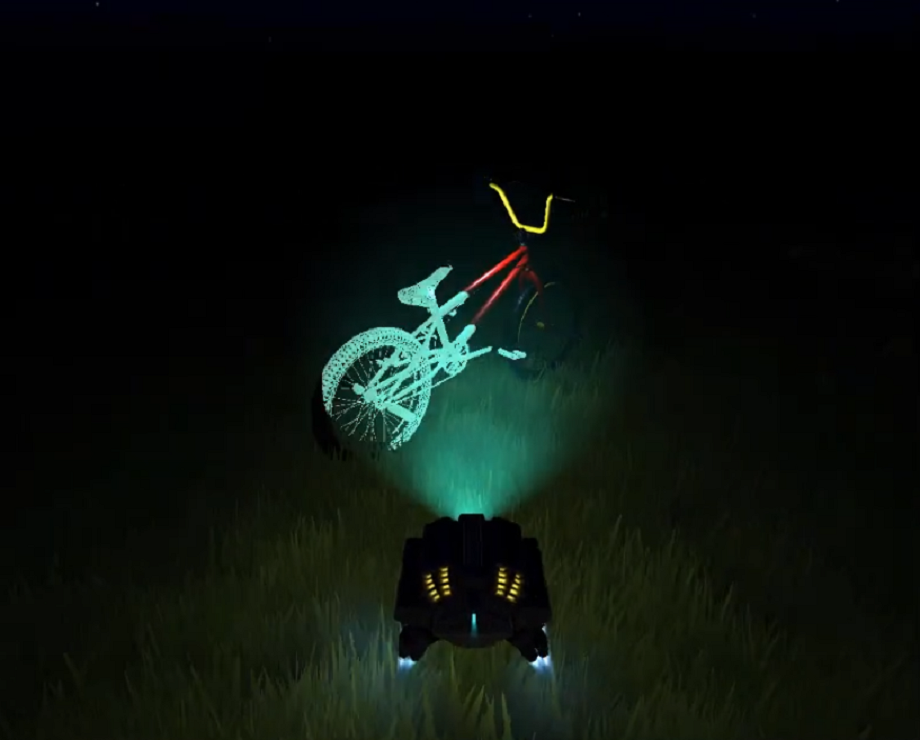
\includegraphics[width=0.32\textwidth]{images/unity-frontpage-drone3.png}}
%         \caption{3D Model of our Explorer Drone, from the Unity Asset Store \cite{unity-asset-store}}
%     \label{fig:frontpage-drone}
% \end{figure}

%  \begin{figure}[!ht]
% \captionsetup[subfigure]{justification=centering}
%     \centering
%       \begin{subfigure}{.49\linewidth}
%         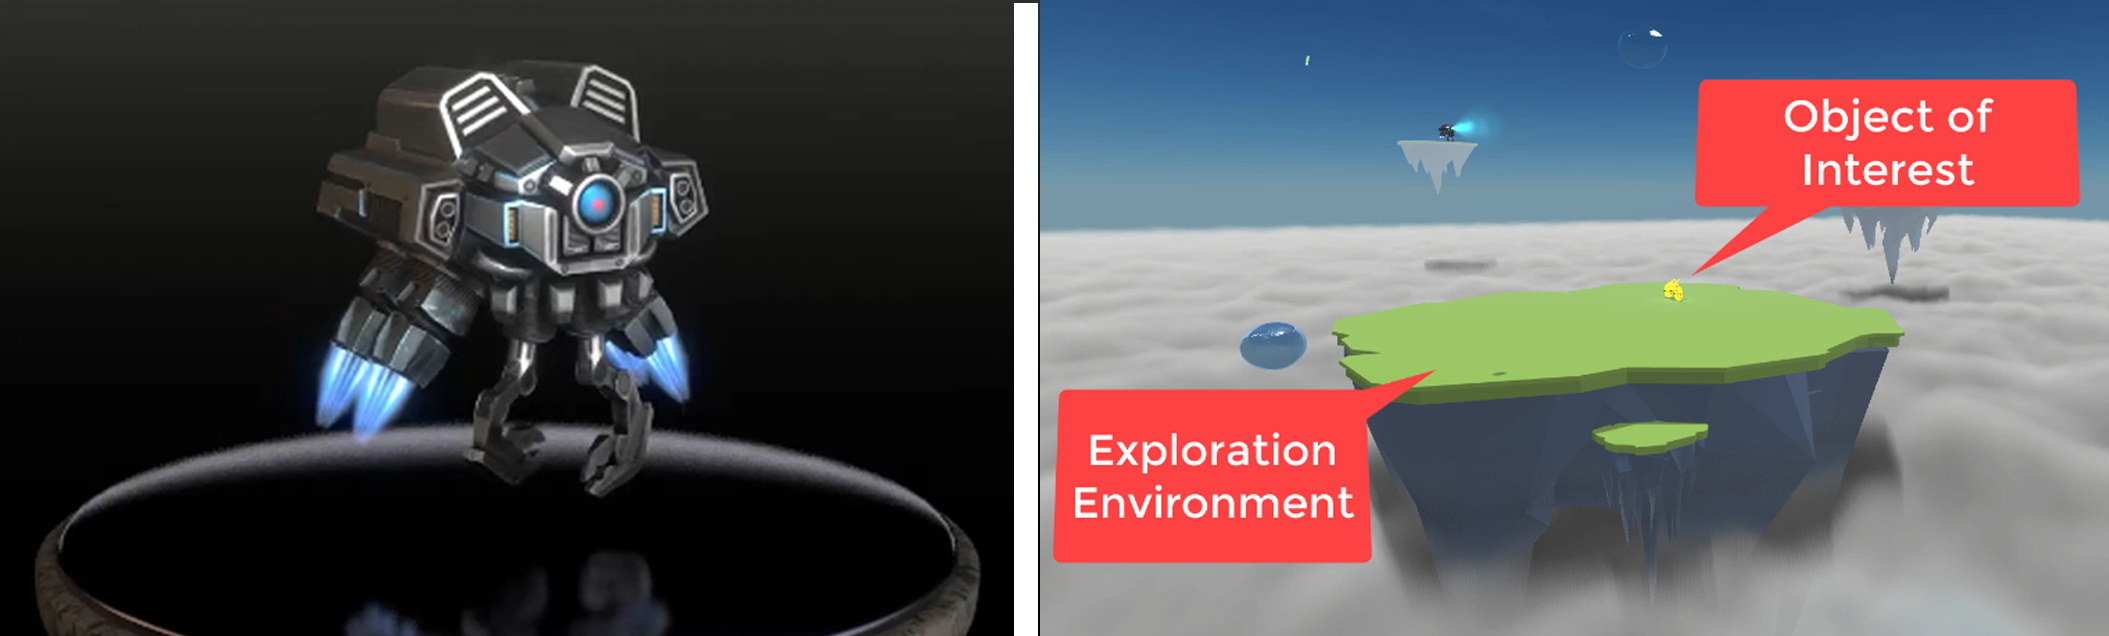
\includegraphics[width=0.5\textwidth]{images/chapter1-figure1.png}
%           \caption{3D Explorer Drone \cite{unity-asset-store} (left) and Training Island (right).}
%           \label{fig:chapter1-figure1.png}
%       \end{subfigure}
%       \begin{subfigure}{.49\linewidth}
%         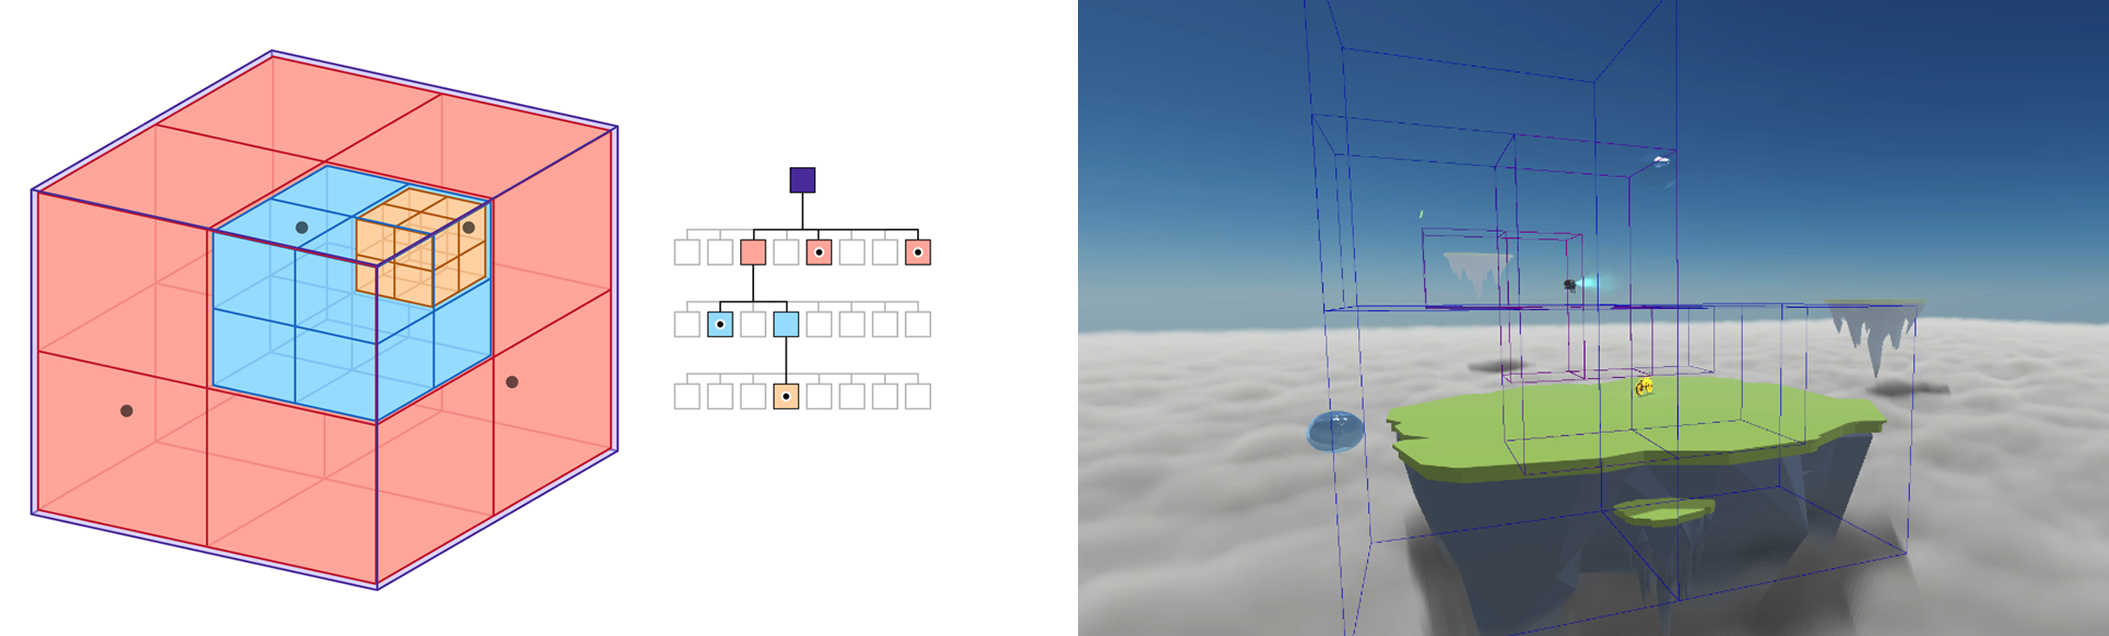
\includegraphics[width=0.49\textwidth]{images/chapter1-figure2.png}
%           \caption{Octree data structure \cite{dulalsaurab_octree} and subdivision \\ of training environment.}
%           \label{fig:chapter1-figure2.png}
%       \end{subfigure}
%       \begin{subfigure}{.49\linewidth}
%         \includegraphics[width=0.49\textwidth]{images/chapter1-figur3.png}
%           \caption{Grid sensor used to enable vision (left). \\ Object of interest and voxel scanner (right).}
%           \label{fig:chapter1-figure3.png}
%       \end{subfigure}
%       \begin{subfigure}{.49\linewidth}
%         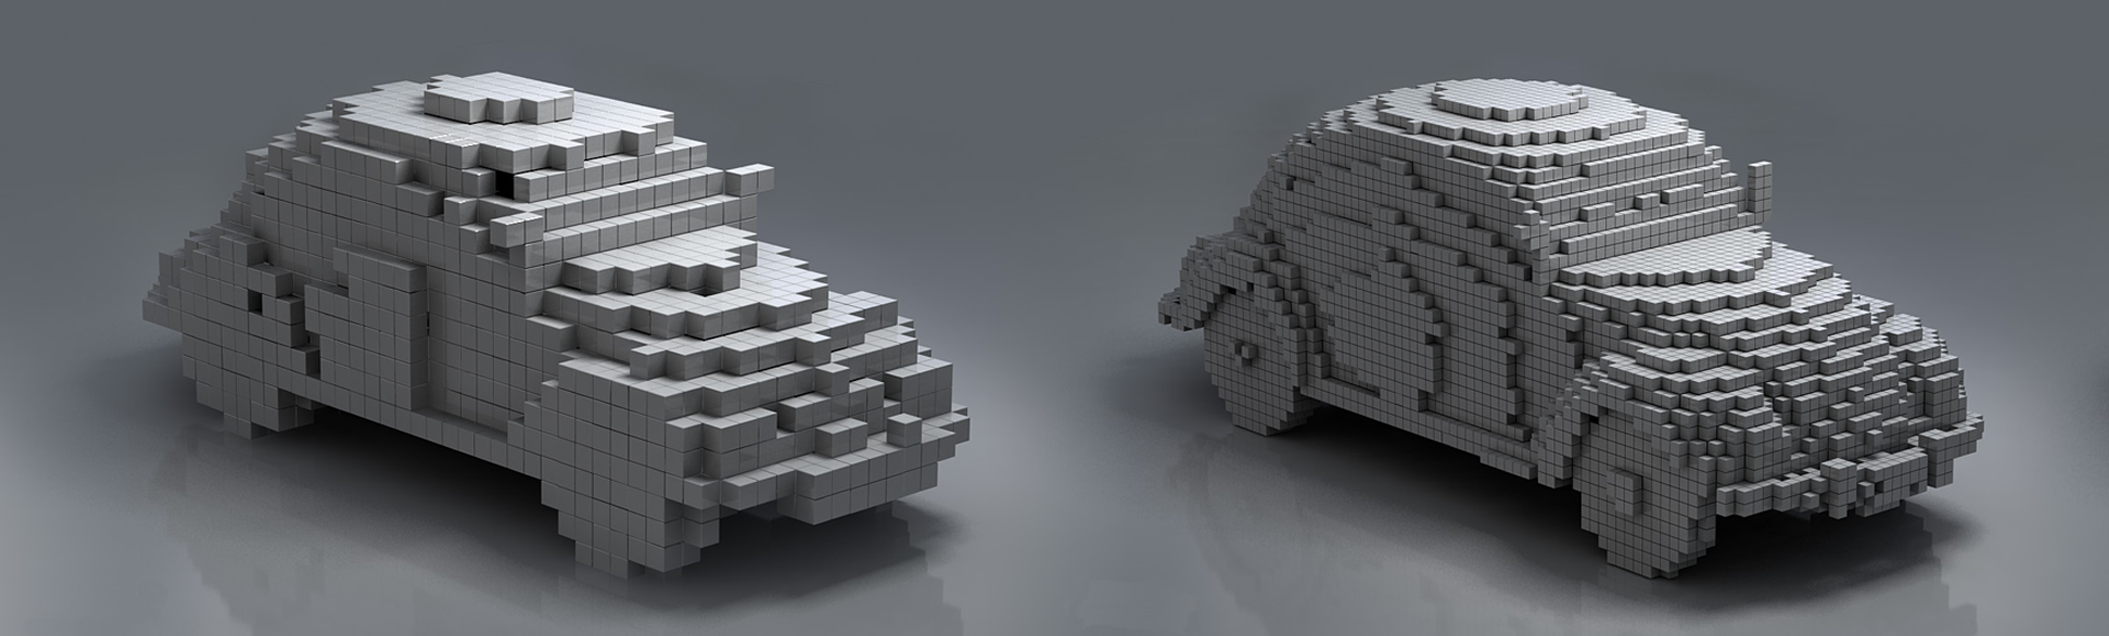
\includegraphics[width=0.49\textwidth]{images/chapter1-figure4.png}
%           \caption{Voxelization of 3D models used to motivate \\ exploration of objects of interest. Taken from \cite{bilderzucht_voxelization}.}
%           \label{fig:chapter1-figure4.png}
%       \end{subfigure}
% \end{figure}



\begin{figure}[!ht]
\begin{center}
    % \subfigure{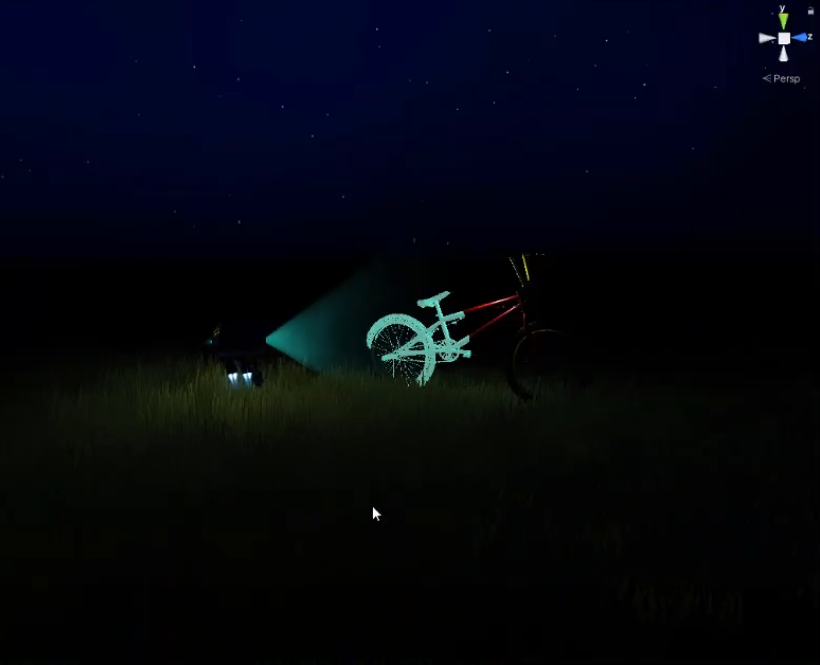
\includegraphics[width=0.315\textwidth]{images/unity-frontpage-drone2.png}} 
    \subfigure[3D Explorer Drone \cite{unity-asset-store}.]{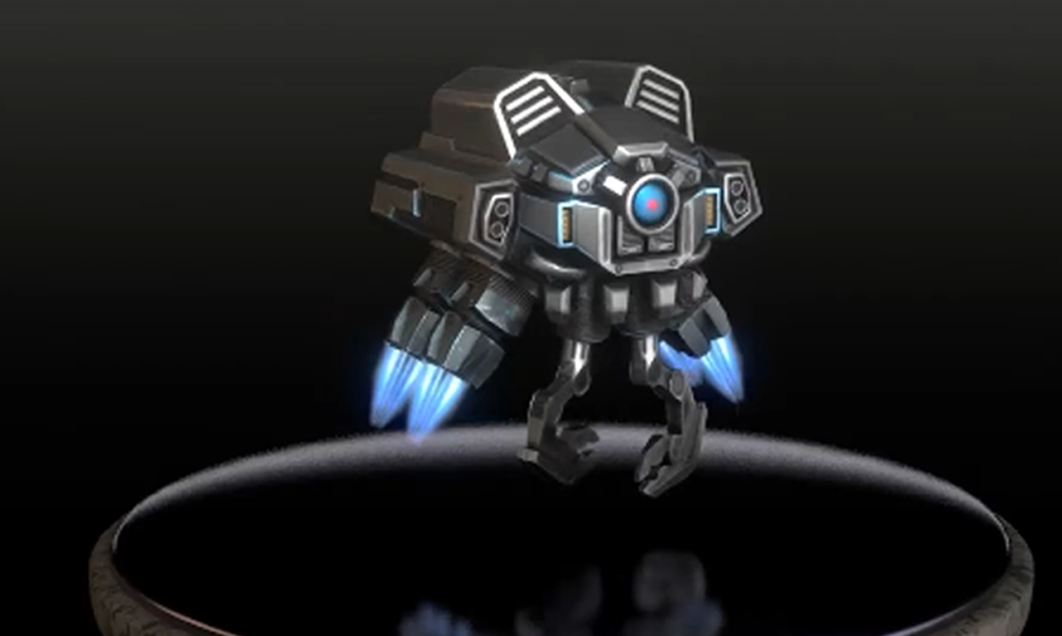
\includegraphics[width=0.245\textwidth]{images/chapter1-small-figure1.png}} 
    \subfigure[Training Island.]{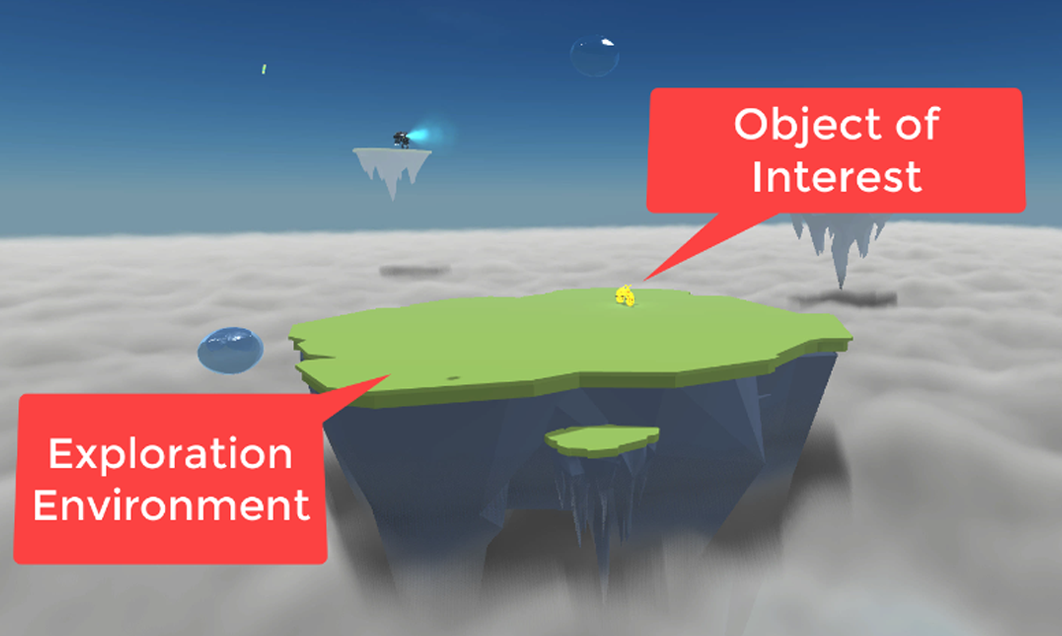
\includegraphics[width=0.245\textwidth]{images/chapter1-small-figure2.png}} 
    \subfigure[Octree data structure \cite{dulalsaurab_octree}.]{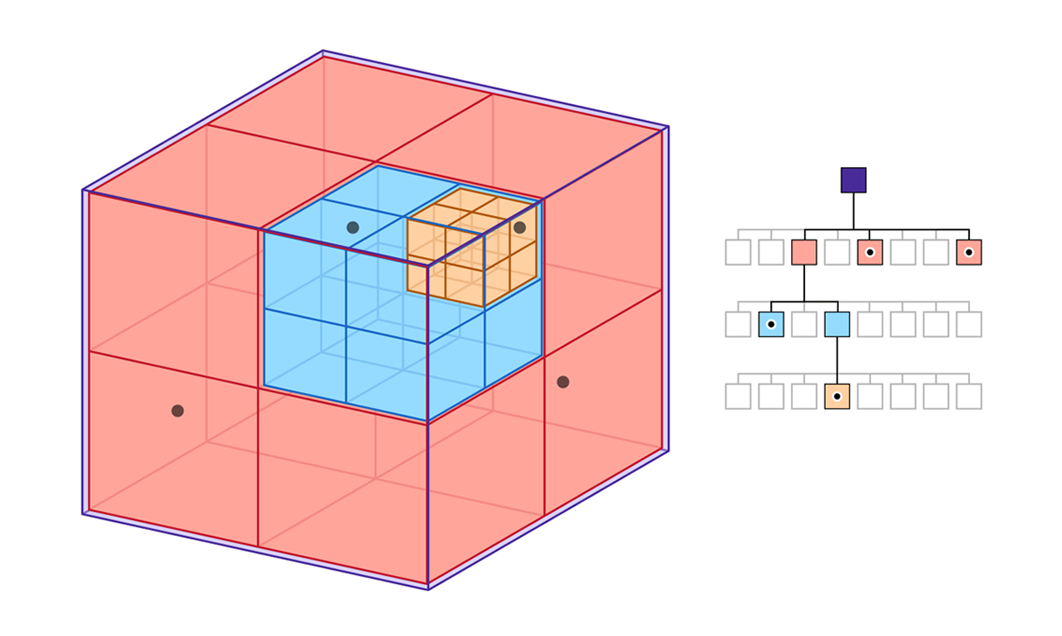
\includegraphics[width=0.245\textwidth]{images/chapter1-small-figure3.png}} 
    \subfigure[Octree island subdivision.]{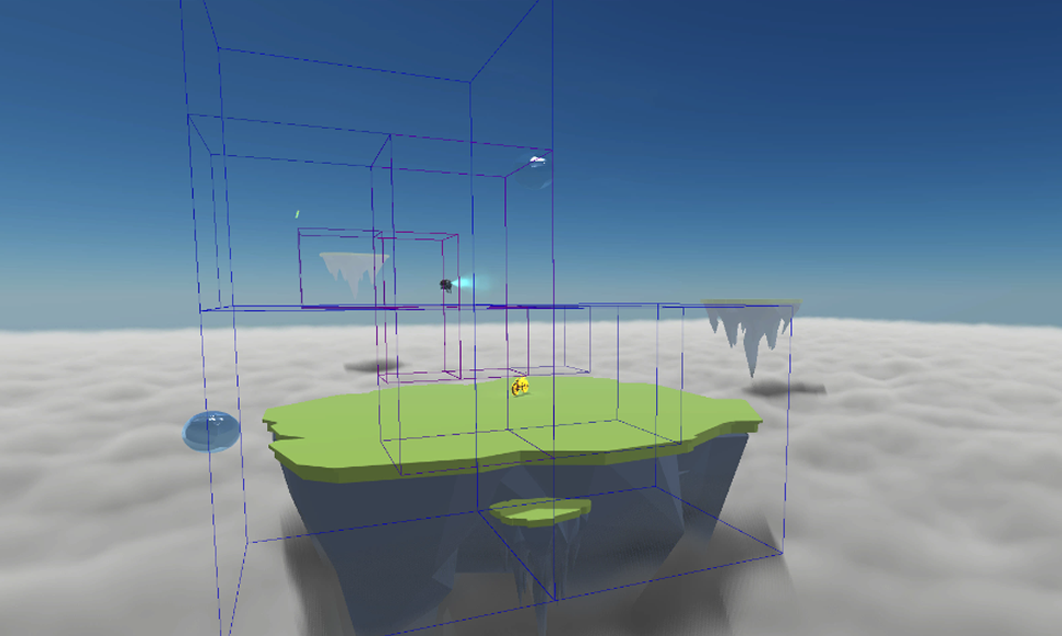
\includegraphics[width=0.245\textwidth]{images/chapter1-small-figure4.png}} 
    \subfigure[Grid sensor for vision.]{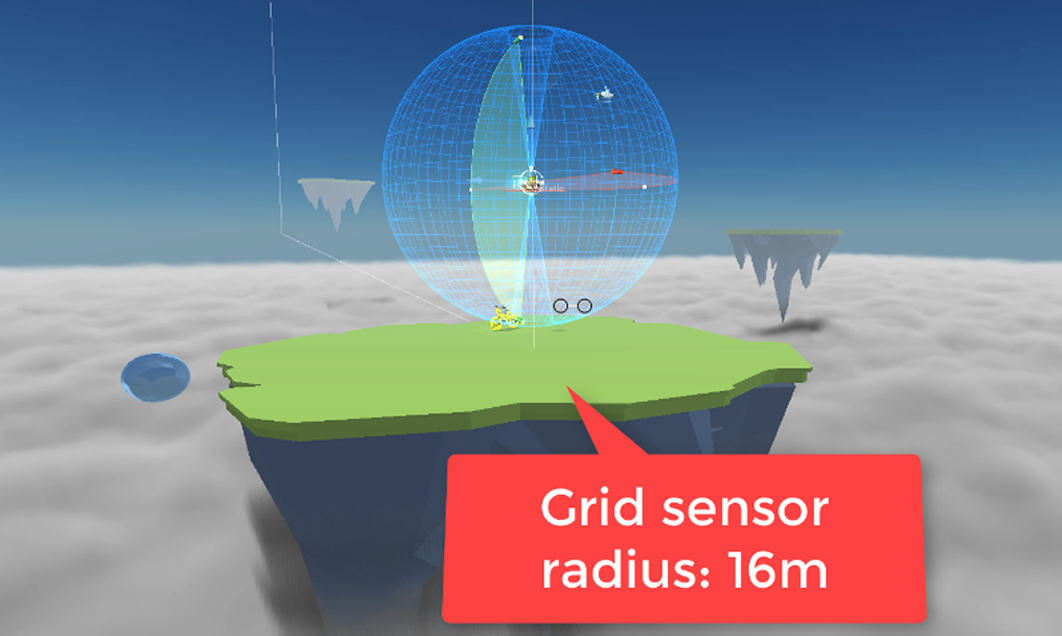
\includegraphics[width=0.245\textwidth]{images/chapter1-small-figure5.png}} 
    \subfigure[Object of interest and voxel scanner.]{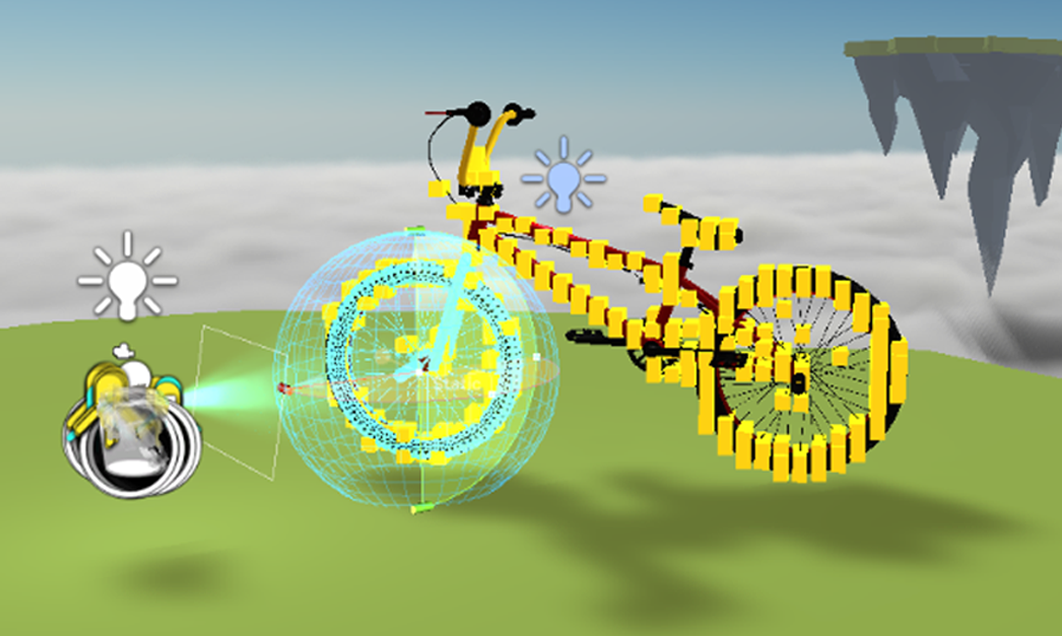
\includegraphics[width=0.245\textwidth]{images/chapter1-small-figure6.png}} 
    % \subfigure[Voxelization used to motivate exploration of objects.]{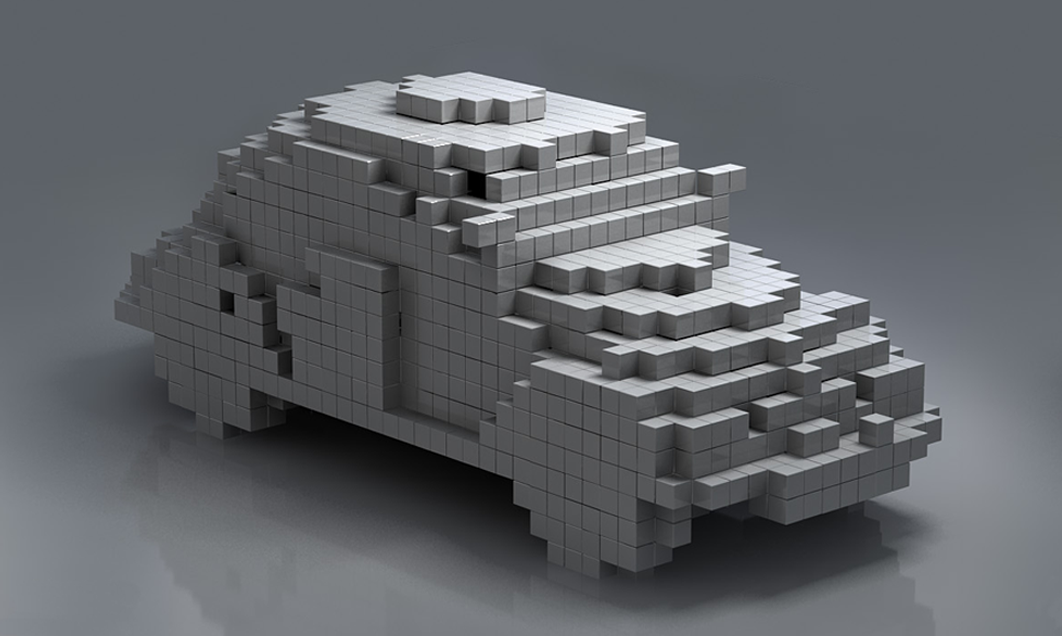
\includegraphics[width=0.25\textwidth]{images/chapter1-small-figure7.png}} 
    % \subfigure[3D Explorer Drone \cite{unity-asset-store} (left) and Training Island (right).]{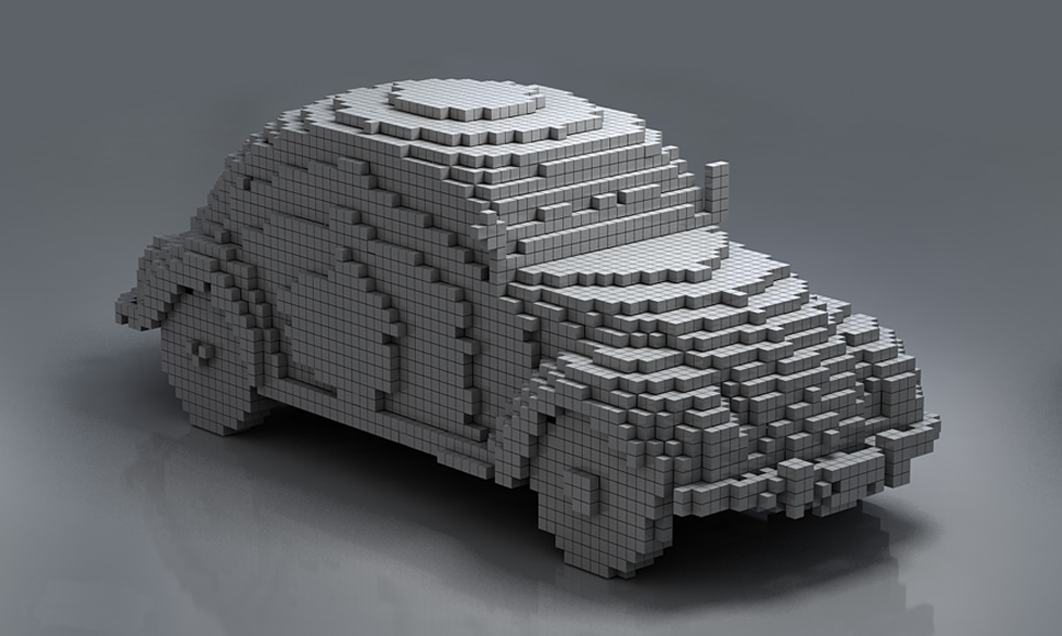
\includegraphics[width=0.25\textwidth]{images/chapter1-small-figure8.png}} 
    \subfigure[Voxelization used to motivate exploration of objects \cite{bilderzucht_voxelization}.]{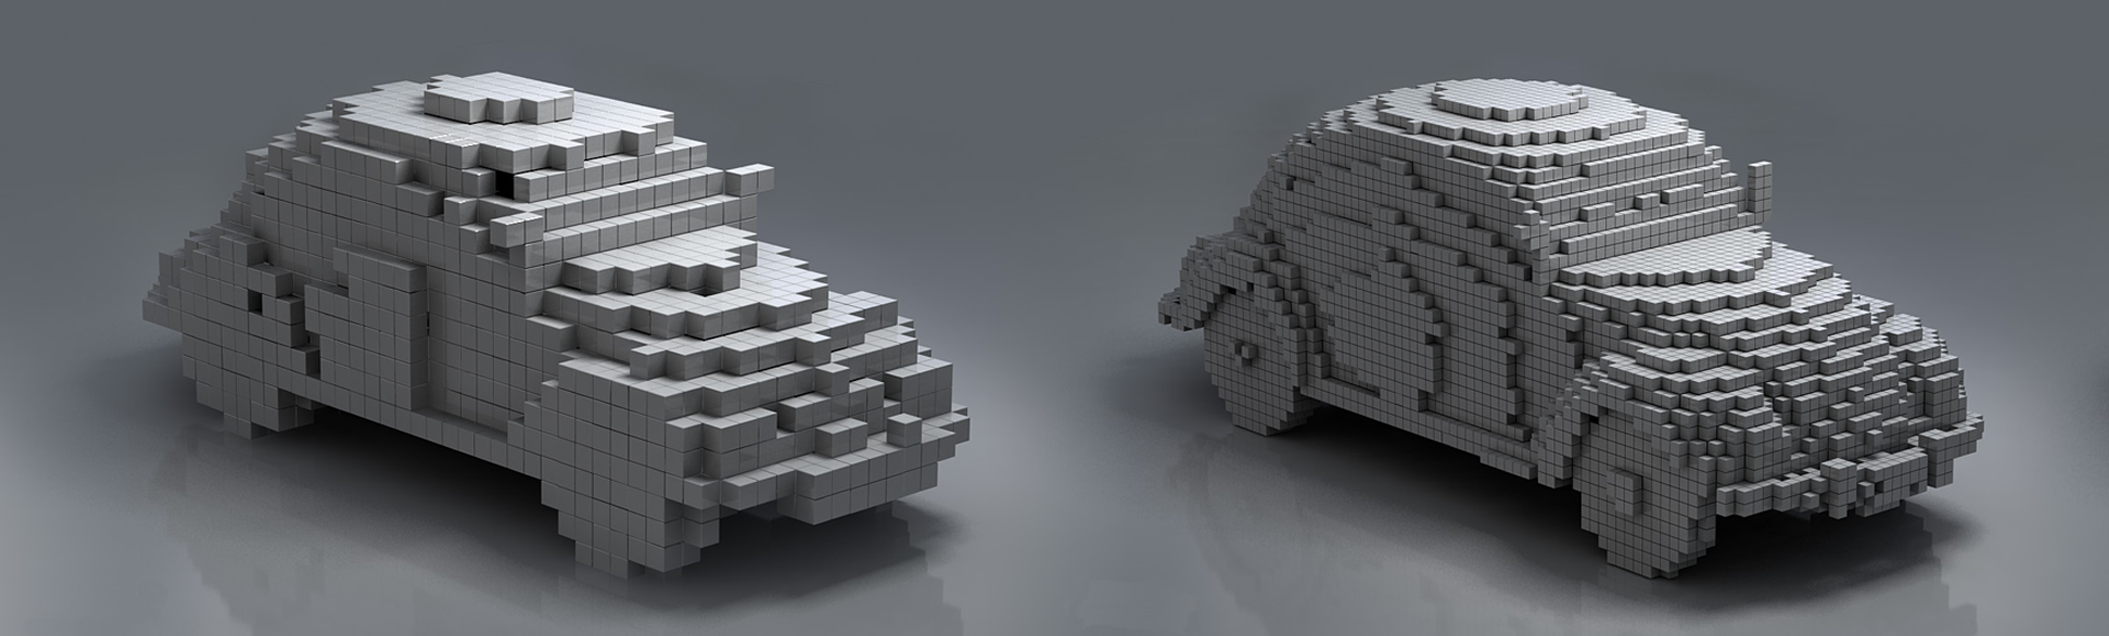
\includegraphics[width=0.49\textwidth]{images/chapter1-figure4.png}} 
    % \begin{minipage}[b]{.5\linewidth}
    % 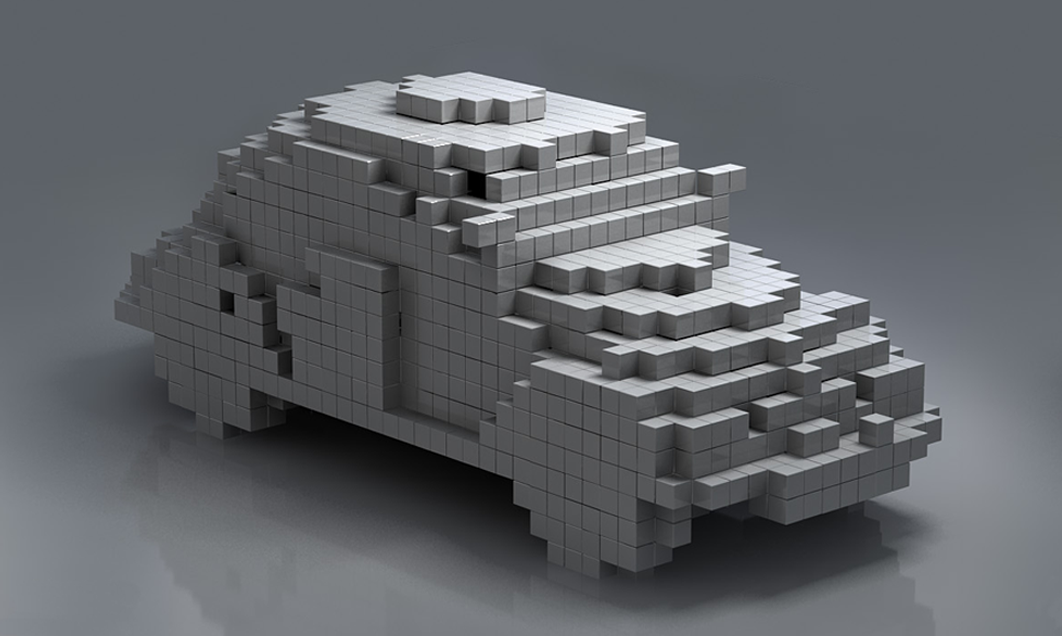
\includegraphics[width=0.49\textwidth]{images/chapter1-small-figure7.png}
    % 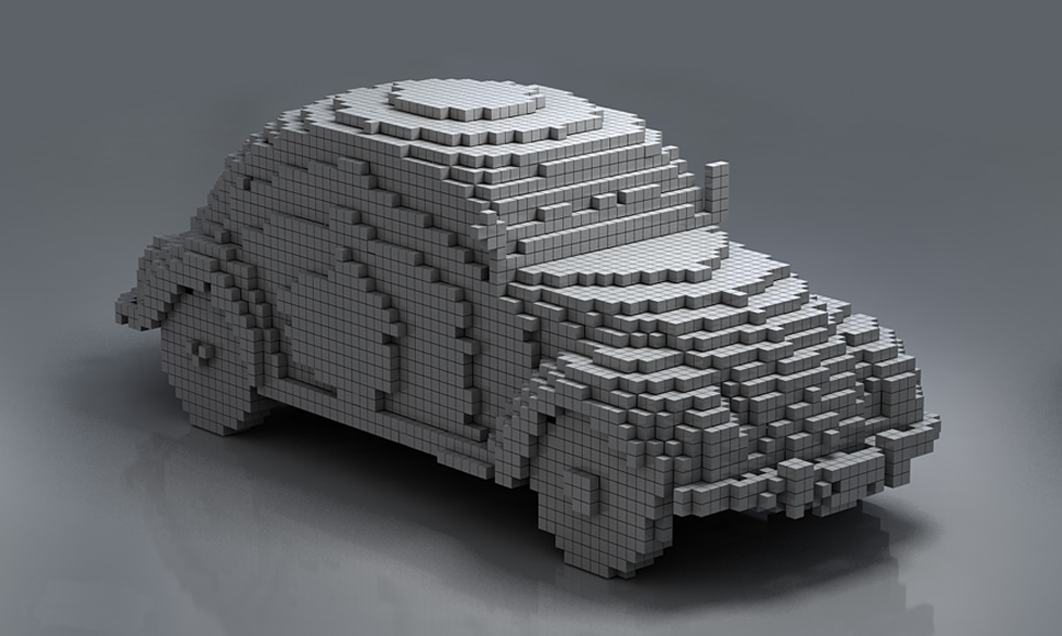
\includegraphics[width=0.49\textwidth]{images/chapter1-small-figure8.png}
    % \subcaption{Voxelization used to motivate exploration of objects \cite{bilderzucht_voxelization}.}
    % \end{minipage}

   
    % \subfigure[ and subdivision \\ of training environment.]{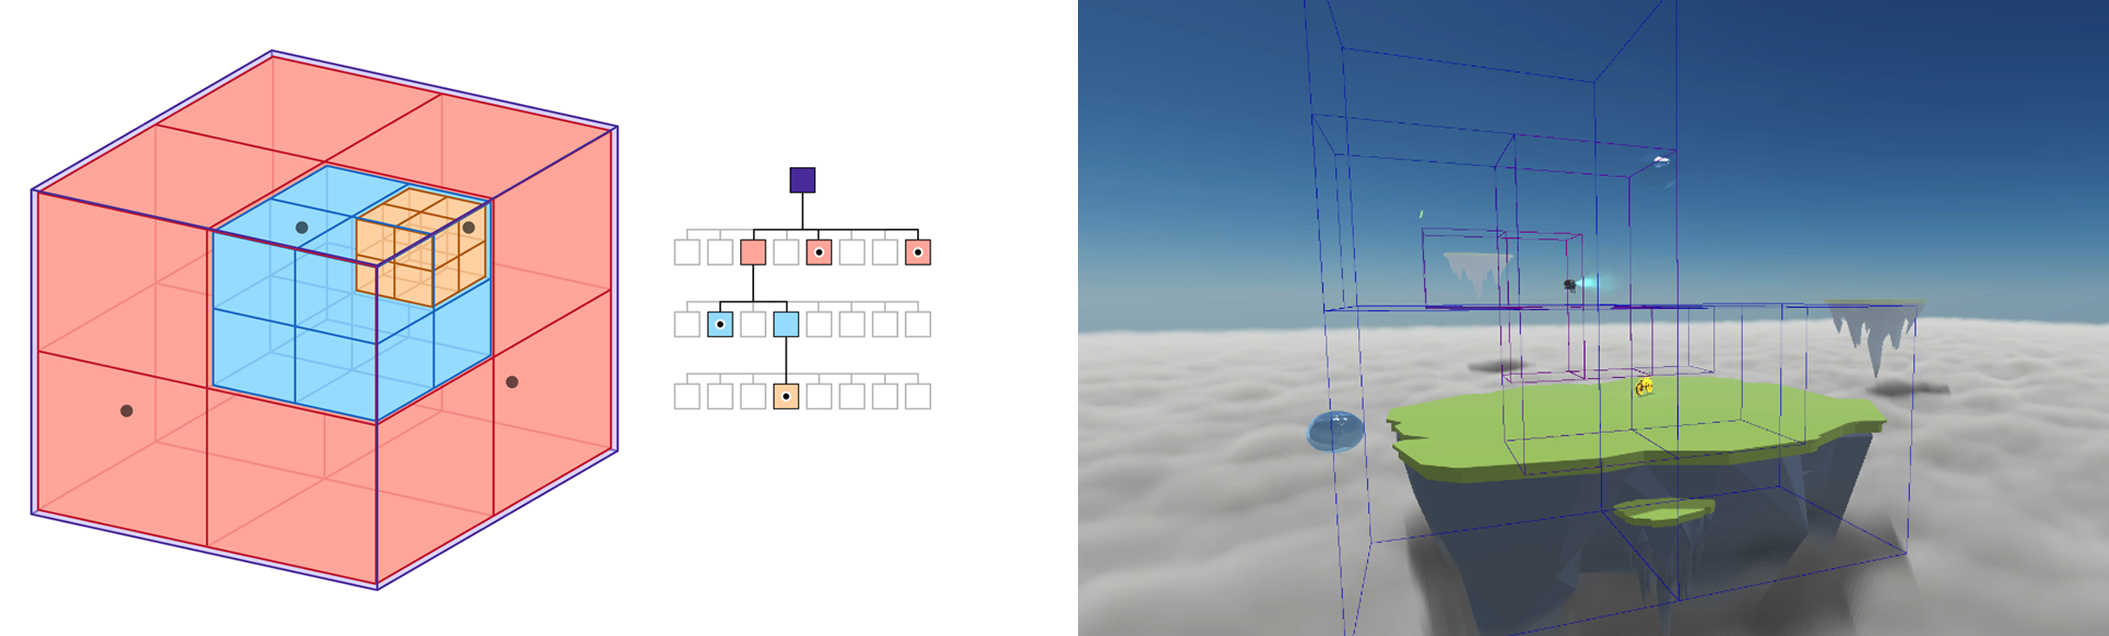
\includegraphics[width=0.49\textwidth]{images/chapter1-figure2.png}} 
    % \subfigure[Grid sensor used to enable vision (left). \\ Object of interest and voxel scanner (right).]{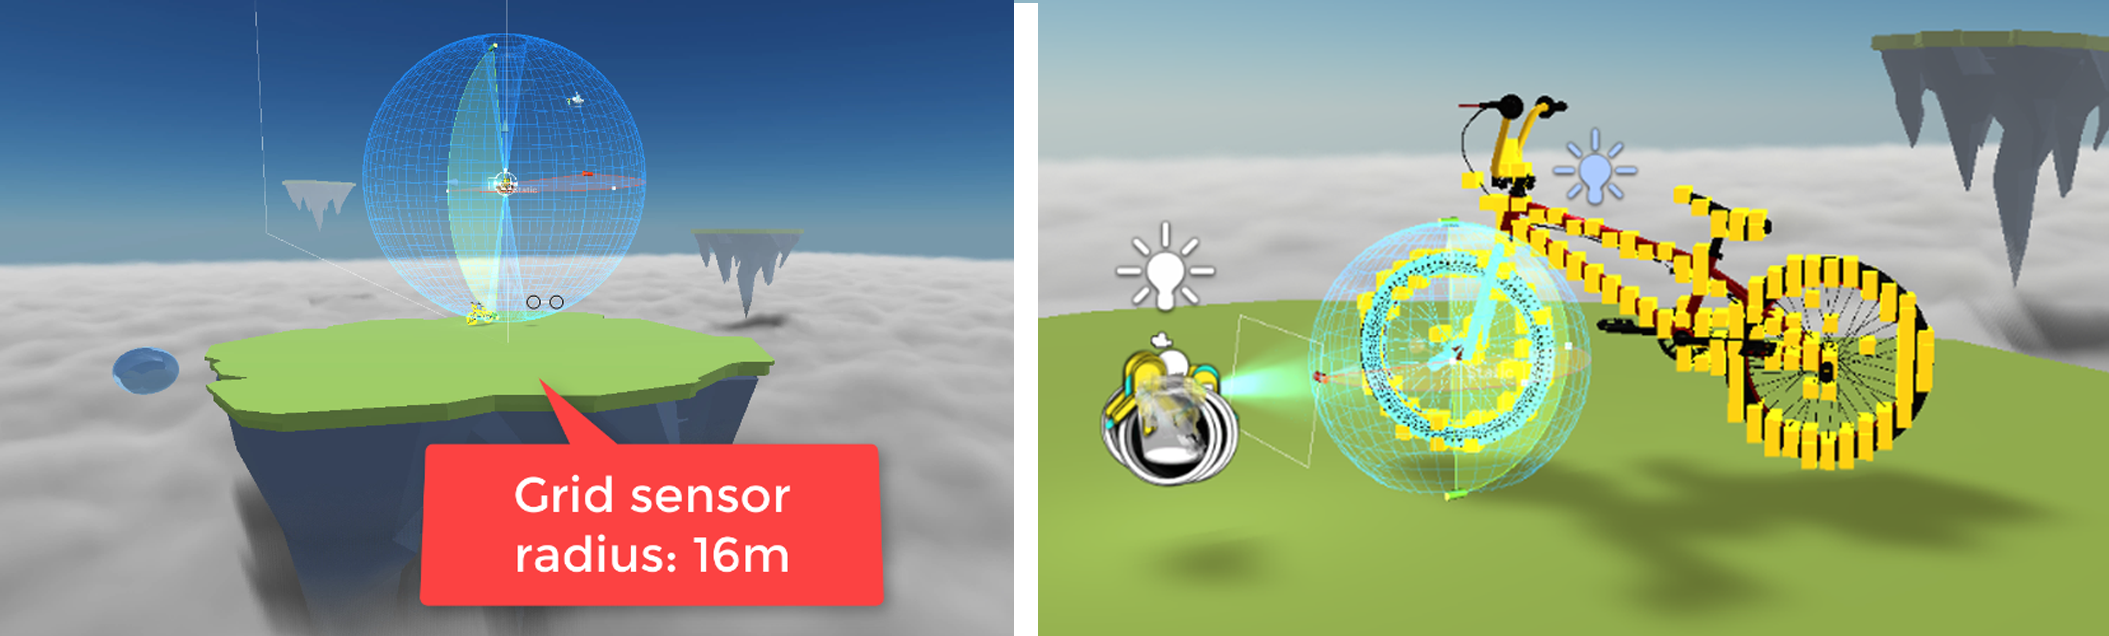
\includegraphics[width=0.49\textwidth]{images/chapter1-figure3.png}} 
   
    % \caption{3D Model of our Explorer Drone, from the Unity Asset Store }
    \label{fig:frontpage-drone}
\end{center}
\end{figure}

\section{Motivation}\label{chap:1:motivation}
% Use Case: Improving the Cow Milking Automation
% - first time scene understanding was done
% - scene understanding today and what value it has for enterprise applications
% - current state of scene understanding
% - limitations / challenges / problems with it

At the NeurIPS 2017, \textcite{abbeel_youtube_2017} presented a video of robots cleaning a living room, bringing a bottle of beer, and performing tasks usually seen in science fiction movies.
Later it was showed that the robot was being controlled by a human with a remote controller: his presentation hinted towards the fact that the robots that we use today are physically capable of performing such actions, so building state of the art robotics is not a hardware problem anymore but a software one.
As of 2021, tasks like teaching a robot how to pick a bottle of beer can still be a very challenging task. Nevertheless, current algorithms have come a long way since Pieter's talk and much has been done to improve robots' understanding of their environment and to study what set of tools are required to achieve not just perception in robots but intelligent agents \cite{kok2020trust, trivedi2008soft}.
Works like DeepMind's recent publication \cite{silver2021reward} hint towards a promising future where reward maximization methods are a promising path towards general artificial intelligence. Where current AI models outperform humans at specific tasks and alleviate repetitive workloads, general AI would potentially outperform humans at nearly every cognitive task. 
It is therefore imperative to continue research in disciplines such as reinforcement learning as it is one of the most promising field to achieve intelligent robotic behavior \cite{abbeel_youtube_2017, kok2020trust, silver2021reward}.

% is of vital importance to to eventually

% most common ML applications people use supervised learning (input, and know what the output is, so we can use an optimization algorithm to compute gradients to train the NN to produce the outputs)
% - (rewrite) In this sense, applications that use these kind of technologies are scarce given the lack of [...] and [...].

% It is believed that the first time a cow was milked was around 8,000-10,000 years ago, somewhere in Europe\cite{valente_2017}. Interestingly, milk also is given the credit for the developments that have happened in the modern food industry. Not only because of how widespread it is in today's culture, but also because of bringing cheese and butter with it. Over the past 8,000 years, more than a handful of technological advancements have happened, specially in the farming industry. The Agricultural Revolution proved to be a turning point for the food supply, allowing the way for the Industrial Revolution \cite{lumenlearning_2021}. Consequently, milking robots have been around in agriculture for over 20 years. However, the concepts of the widespread milking systems available on the market have hardly had any adaptations leveraging the latest technological advancements. The current largest supplier, Lely, still uses electro-pneumatic spindle motors even in the latest version of the milking robot (Astronaut A5). The benefit of these motors is their low cost and their physical compliance, making them resistant to cow kicks. They require, however, a lot of maintenance. For example, the seal of these motors must be replaced regularly so that the system remains operational. As of today, the herd size in Swiss farms is often big enough so that more than one milking robot would be needed, but the space requirements do not allow for this without having to remodel the barn's infrastructure.

% TODO adapt this part to be in line with scene understanding

Accordingly, a current project at ZHAW linked to this thesis work aims to construct a milking robot that leverages machine learning methods to outperform traditional milking robot technologies, in cooperation with the industrial partner Sutter Landtechnik GmbH (SLG).
Most of today's milking robots use a 2D laser scanner to estimate the position of the cow, the udder and the cow's teats, and several measurements are necessary. This is time consuming and if the cow moves during the measurement, the position estimation must be reinitialized. ZHAW therefore proposes innovative changes to the milking robot's architecture, using electric drives and a more compact kinematic structure. Moreover, given that inexpensive 3D cameras have been introduced to the market over the past few years, it is now possible to leverage high resolution 3D point clouds to dynamically estimate the position of the cow teats while also reducing the costs of manufacture. 

This thesis aims to contribute to this project but also to the fields of practical reinforcement learning, computer vision research and practical machine learning. To this end, we study the scenario where given a milking robot defined as an unknown environment with objects of interest, a reinforcement lerning agent's task is to explore such an environment and the objects in it.
% the milking robot problem represents an unknown environment where not only the position of objects is of interest, but the general level of awareness of the overall environment itself.
In other words, the aim of this masters thesis is to select and implement a computer vision enabled pipeline that leverages active vision to reduce the uncertainty over time in a new environment, one of which can be a milking robot's environment. In this sense, uncertainty is defined as the temporal semantic entropy given by an object detector and the derived class complexity through the Shannon entropy. 

The proposed solution is inspired by the human brain's physiology and approximates the discovery process a human would follow in an unknown environment and it leverages the concept of temporal semantic entropy proposed by \textcite{chaplot2020semantic} to define this dimension of uncertainty. Concretely, the task at hand is an exploration task for coverage maximization with a novel approach that leverages extrinsic rewards from voxel scans constructed from ubiquitous RGBD information. From the perspective of architecture design, it proposes a pipeline that can be further extended to a multitude of use cases and even other semantic models, in an attempt to contribute to the research on semantic-curiosity-motivated exploration.

Finally, while there are increasingly more 3D datasets out there for benchmarks on computer vision tasks, reinforcement learning algorithms have seen themselves limited to black box environments and popular games such as Atari 2600, Quake III, Doom, Minecraft and Gazebo simulations. However, as deep reinforcement learning algorithms become more sophisticated, new environments and benchmarks must emerge since existing environments and benchmarks based on them become less informative \cite{juliani2018unity}. This work contributes to existing agent testing environments with three 3D Unity-based scenarios, which are easy to extend to further use cases. They also differentiate themselves from traditional benchmarks by being developed with improved realism, which aims to close the gap between synthetic and realistic data. These environments are used to further evaluate the exploration task at hand and the feasibility of knowledge transfer across environments. All of this leaves the door open for future research in simulated applied vision systems and for in-robot implementations of the exploration policies studied.

% Based on this background, the aim of this Masters thesis is to select and implement a machine learning and computer vision enabled pipeline that estimates the 3D pose and direction of cow teats. The methods proposed in this work build the basic structure for an approach to estimate the position of the cow teats.



% Unity: A General Platform for Intelligent Agents
% As deep reinforcement learning algorithms become more sophisticated, existing environments and the benchmarks based on them become less informative. For example, most
% environments in the ALE have been solved to above human-level performance, making the
% continued use of the benchmark less valuable (Machado et al., 2017; Puigdomènech Badia
% et al., 2020). A complementary point created by this state of algorithmic progress is that
% there exists a virtuous circle in which the development of novel environments drives the
% development of novel algorithms. We can expect the research community to continue to
% provide high-quality algorithms. However, it is unclear from where researchers should expect
% high-quality environments, since the creation of such environments is often time-intensive
% and requires specialized domain knowledge. This continual need for novel environments
% necessitates an easy-to-use, flexible and universal platform for unrestricted environment
% creation.
% Simulated environments are constrained by the limitations of the simulators themselves.
% Simulators are not equal in their ability to provide meaningful challenges to learning systems.
% Furthermore, it is sometimes not obvious which properties of an environment make it a
% worthwhile benchmark for research. The complexity of the physical world is a primary
% candidate for challenging the current as well as to-be-developed algorithms. It is in the
% physical world where mammalian and, more specifically, human intelligence developed, and
% it is this kind of intelligence which researchers are often interested in replicating (Lake et al.,
% 2017).

% Although this requires much more complex data processing on a powerful control system, it does away with a time-consuming, separate 
% time-consuming, separate measurement process can be dispensed with. Dynamic measurement with modern sensors also offers the potential to be much more robust and reliable than the measurement methods used today.
    
    % \begin{itemize}
    %     \item describe the general need for automated cow milking
    %     \item describe how the problem is currently being solved briefly
    
    %     \item describe the challenges in cow teat recognition: morphology/shapes and movement
    %     \item describe how these methods fail || describe challenges/limitations of current methods (sensors, etc, no memory)
    
    %     \item can solve this problem with computer vision briefly
    
    %     \item describe cow project main driver (The InIT's purpose) (do we mention how expensive current solutions are?)

    % \end{itemize}
% \section{The Need for Organic Milk}\label{chap:1:organic-milk}

% In recent years, the financial pressure on agriculture in Switzerland has increased massively. Since 1980, the number of farms has been shrinking by about 1000 farms per year. The Swiss consumer wants more and more organically grown products and at the same time consumer prices are getting cheaper and cheaper. The extensive Swiss animal welfare regulations, which are the strictest in Europe, make animal husbandry even more expensive. All this leads to the fact that the average income of a farmer family decreases annually. The farmers' association is therefore calling for greater support from the state. The SLG sees the key to running a profitable Swiss farm not in higher government subsidies, but in a more efficient machine park, which is specifically optimized for the Swiss market, according to Swiss legislation and for organic and ecological farming. All robotic milking equipment available today is not designed for organic farming but optimized to maximize milk yield. However, in the saturated Swiss milk market, what is needed is not more milk, but rather milk produced in a fair, organic and cost-efficient way.

% Across Europe, organically produced milk is still a niche product. However, the SLG is convinced that this will change in the coming years, as consumers in Europe are also paying more and more attention to what they eat and how their food was produced. The focus of a new development should therefore not be on maximizing the amount of milk per animal, but on minimizing investment and operating costs, and above all, these new systems should enable organic farming without compromise. This starts with giving cows access to pastures.

% Today's robotic systems are designed for 24/7 operation. Especially for smaller farms, this mode of operation is necessary to keep operating costs low. In contrast, an important feature of the new robotic system is to be able to milk all cows on a farm within one to two hours, thus combining all the advantages of a conventional milking parlor with the benefits of a milking robot. For this purpose, the new robot is dimensioned in such a way that several robot arms can be installed in the intermediate aisles of existing barns without the need for major cost-intensive building adaptations. By installing the robot in the intermediate aisles of the barn, it will also be possible to minimize the use of concentrated feed, as the cows will automatically pass the robot when moving from the cubicles to the feeding axles.


\section{Purpose and Research Questions}\label{chap:1:research-question}
% In this work, a machine learning and computer vision based solution will be used to estimate the pose of cow teats for a milking robot. Regarding this task, this work tackles the following research question:
% How can the cow teats 3D pose be estimated under 10 seconds?
In this work, the problem of uncertainty in an environment presented by the milking robot is looked from a more general perspective. We therefore look at exploration policies that can also contribute to a plethora of other use cases. More concretely, we propose a reinforcement learning based solution to explore a 3D scene and the objects in it. To this end, we use extrinsic motivation while also leveraging the uncertainty in the environment to adapt such behavior.
% maximize coverage in a 3D scene, using extrinsic motivation to pursue new states.
% new environments. 
% Moreover, it takes into account uncertainty in the environment, defined by the temporal inconsistencies in an object detector as a supporting exploration metric. 
Finally, a set of research scenarios are proposed to show the versatility of our exploration policies and contribute to existing benchmark environments. 
% and account for realism using Unity 3D
Regarding this task, this work tackles the following research questions:
\begin{itemize}
    %  Howcan an active vision exploration policy based on a ubiquitous source of information such as voxels, in currently accessible RGBD cameras, contribute to reducing the uncertainty about a scene?
    % \item How can voxel structures be exploited for intrinsic motivation in active vision exploration policies?
    % \item How can uncertainty, defined through semantic entropy, be used to thoroughly scan objects through active vision policies?
    % \item How can active vision exploration policies be leveraged for a practical scenarios, beyond the original milking robot use case? 
    % 3D data (meshes or point clouds), in voxel form, be exploited for extrinsic motivation of objects?
    \item How can an embodied agent increase the overall certainty about an object's characteristics, i.e., how can trajectories around objects of interest be generated to reduce the uncertainty about such objects? 
    \item How can these objects be found in large and unknown environments by the same agent?
    % \item How can uncertainty be defined through semantic entropy and be used as a motivation in exploration policies?
    
\end{itemize}

\section{Approach and Methodology}\label{chap:1:approach-methodology}
This work focuses on leveraging reinforcement learning techniques to manipulate an agent (camera) motivated by abstractions of the perceived environment. These abstractions are meant to simplify the complexity present in the environment and take the form of translations of camera input into voxels. Voxels, accordingly, represent the direct goal for a scanning agent to obtain view from an object from multiple angles. The problem that is further studied within this master's thesis is two-fold: 1) uniform exploration of large open spaces and 2) thorough scanning of objects from multiple angles, as a mean to reduce the uncertainty in a 3D scene over time. We define, therefore, uncertainty through the semantic entropy observed at a given point in time, which is inspired by \textcite{chaplot2020semantic}.

The strategy taken for this project work is the following:

A state of the art analysis was done to propose a set of exploration policies using reinforcement learning that answer the research questions. 
First, this analysis includes the evaluation of related efforts in scene understanding, active vision, and RL-based exploration.
% variety of advancements in computer vision and machine learning fields such as 3D data representation, object detection, scene understanding, and reinforcement learning techniques for the manipulation of a vision-driven agent for exploration.
% pose estimation for the 3D pose estimation of cow teats.
% This also includes the implementations of the proposed algorithms and the respective optimization of their parameters to solve the task optimally. 
Second, it includes implementations of exploration policies and the respective optimization of the learning environment and the learning agent and its algorithm to solve the task optimally. 
It is also important to note that this process has an iterative nature, where the validation of the models' results triggers changes for optimizations in the learning environment and the agent, 
% , and the diverse algorithms' parameters
in order to achieve the best possible results. The used data is of synthetic origin, and was modeled, assembled and simulated in the Unity game engine. Finally, the results were critically evaluated and compared to a set of baselines. The generalization capabilities, reliability and limits of the results are then discussed and further improvements on this field considered. 
%  further work: using semantic queues, implementing full pipeline using RGB to measure how computation heavy the voxel calculation could be and optimization strategies, a.k.a. out of scope limitations that will only be discovered when the actual voxel manipulation is done (work by RoutedFusion and seems promising to work on scans). 

\section{Contributions}\label{chap:1:contributions}
Our contributions can be summarized into the following points:
\begin{itemize}
    \item We build upon knowledge acquired through a previous publication, namely \textit{\citetitle{DBLP:journals/corr/abs-2105-09843}}\cite{DBLP:journals/corr/abs-2105-09843}
    and the Bachelor's thesis \textit{\citetitle{dano}}
    , to propose a novel voxel-based exploration method, which builds upon model-free
    % to the best of our knowledge
    reinforcement learning
    % to enable visual-agnostic exploration
    and accounts for the abstract concept of "uncertainty" in an environment, defined through the amount of different object classes present in such an environment. This definition is known as "semantic entropy, or as "the inconsistencies in the temporal class density", as inspired by the concepts presented by \textcite{chaplot2020semantic}.
    
    \item We demonstrate that our method outperforms our Unity implementations of classical and geometric exploration for scanning strategies, and further improves upon exploration methods motivated by coverage maximization \cite{chen2019learning} using octrees and adapts its exploration pace through semantic entropy.
    % , which is inspired by \textcite{chaplot2020semantic}'s semantic curiosity. 
    
    \item We show that Proximal Policy Optimization (PPO), with minimal hyperparameter tuning and any domain-specific algorithmic changes or architectures, achieves final performances comparable to the Soft Actor-Critic algorithm \cite{schulman2017proximal}.
    % where  synthetic data and real data for the exploration of 3D environments
    \item By using voxels and grid sensors for extensive exploration, our method abstracts the complexity in the 3D world through voxels and therefore is capable of visual-agnostic exploration and transfer learning tasks. 
    % data distribution plays a key role in the performance of transfer learning techniques trained on synthetic data and tested on real robots, enabling the agent to adapt to new environments without changes in its behavior.
    
    \item We evaluate our approach through relevant statistics for exploration and for thorough scanning of objects, where a set of baselines is defined and used to perform the evaluation, inspired by \textcite{darpa_subterranean_challenge}.
    
    \item We further demonstrate that our method excels in new 3D scenarios that represent real life situations where exploration time is critical to save not just time and costs but, more importantly, lives and further losses. 
    
    \item We present the capabilities of Unity-based environments for the development of new benchmarks and its compatibility with the OpenAI gym platform \cite{openaigym} and trainers from Stable Baselines 3 \cite{github-dlr-rm-baselines3}. 

    \item Finally, we demonstrate that an agent equipped with panoramic vision outperforms agents with ordinary monocular vision in the given exploration task, inspired by \textcite{rill2021collision, wojek2012monocular}.
    % Finally, with an ever increasing amount of algorithms, traditional benchmarks become uninformative and allow room for the creation of newer ones capable of testing more sophisticated challenges, representative of the real world. Motivated by recent works in the Unity 3D engine, we contribute three hyper-realistic 3D environments that can be extended for the creation of new benchmarks, testing of new exploration methods and for a variety of other tasks such as synthetic data generation, autonomous driving, exploration, navigation, point-to-goal tasks, etc. The code base for our method can be found at \url{https://github.com/Ademord/ma-unity}.

\end{itemize}

\section{Scope and Limitation}\label{chap:1:scope}
Due to the time constraints, some limitations were laid out to ensure the work was finished within schedule.
\begin{itemize}
    \item The approach used focuses on the manipulation of synthetic data, namely, 3D voxels in the Unity Engine, while the manipulation of point clouds to generate these voxels is left out. This allows the masters thesis to focus on the research on exploration policies for scanning of objects than on computer vision methods for point cloud manipulation.
    \item This work focuses on the results observed in computer vision and machine learning approaches limited to models compatible with the Unity Engine (ONNX implementations). Other techniques, which for example, use lasers for 3D scene understanding, are not taken into account.
    %  this two points are new: one is a new requirement and the other one is the generalization not to just cows
    \item Methods mentioned in \ref{chap2:related-work} sample data from diverse exploration trajectories to then train and compare a semantic detector's performance. They then indirectly evaluate the performance of each exploration policy. This work does not take into account supervised nor unsupervised training of semantic vision networks (segmentation, recognition) given the time constraint. 
    \item This work focuses on scene understanding and camera manipulation techniques using reinforcement learning in the game engine Unity 3D.
    % \item This work will focus on the 3D object recognition of cow teats for milking robots.
    % \item 
\end{itemize}
\section{Target Group}\label{chap:1:target-group}
One one hand, this work is of special interest for researchers in the field of computer vision, reinforcement learning, and Unity using ML-Agents. This is due to the fact that 3D understanding and environment discovery is still a rapidly growing field.  
On the other hand, as demonstrated in the practical application of the proposed method in Chapter \ref{chap:discussion}, a broad audience in the industry is the public interest for this work, such as security and rescue offices, warehouses, factories, where dedicated the scanning of objects for quality assurance or cues in a traffic accident, fires or other unexplored scenes is of special priority. 
This can also be extended to other modules such as data collection pipelines, semantic modules, airport robots, hospital robots, etc.
% for example, to industries where scanning of objects for quality assurance is important.
% Third, as mentioned in \ref{chap:1:motivation}, the industrial partner Sutter Landtechnik GmbH (SLG) is the private interest group for this research.  This is because SLG not only offers sales, installation, and service of technical equipment and machinery for various tasks in agriculture, but also act as a distributor of milking technology, including robots of the "Astronaut" variant \cite{2021lely-a5}.
% It is based in in Andwil and Muolen, Switzerland.
% Its customers are farms of various sizes in German-speaking Switzerland and in nearby foreign countries. 
% , manufactured by the Dutch company Lely. 


% In addition to the areas of tractors and agricultural technology (e.g. harvesting machines), farm technology (barn equipment), there is the area of milking technology, which, in addition to milking machines, includes cooling technology and, last but not least, milking robots. 

% Various machines, including milking technology, were developed by SLG itself and are also manufactured in its own plant. Of the approximately 50,000 farms in Switzerland, about 2,000 are customers of SLG. In addition, there are about 200 farms from nearby foreign countries. With these, SLG generates an annual turnover of ~6.3 MCHF (2018) with its 25 employees. All milking robot systems installed and/or maintained by SLG are of the "Astronaut" type from the Dutch company Lely.

% As the Lely company was not interested in product adaptations for the Swiss market, SLG terminated its direct business relationship with Lely in 2016 and decided to develop its own robotic system. Therefore, in this project, the prototype of a low-cost, modern milking robot suitable for the specific Swiss requirements will be developed, which can be manufactured and marketed by Sutter Landtechnik GmbH (SLG) itself.

% The Lely company with the Astronaut model range has been able to establish itself on the European market for a variety of reasons and is by far the market leader. The European market is dominated by two brands, Lely 55\% and DeLaval 30\% of the market. In Switzerland there are currently around 850 Lely Astronaut and around 300 DeLaval VMS milking robots in operation. The Swiss market is clearly dominated by Lely with a market share of about 72\%. The weak competition, as well as the small Swiss market in relation to Europe, means that specific adaptations only for the Swiss market are not worthwhile for the large groups.
%  computer vision, machine learning approaches, 3D object recognition, point cloud segmentation, point cloud registration, scene understanding, and reinforcement learning

\section{Outline}\label{chap:1:outline}
The following Chapter 2 covers the Foundations for this work, which starts with the related efforts in the fields that this work touches upon. Then it presents the related concepts from octrees, scene understanding, 3D environments and reinforcement learning. Accordingly, concepts related to computer vision, such as history, 3D object recognition, point cloud segmentation, etc., are pushed to the Appendix, to concentrate in the immediately necessary content. Chapter 3 describes the methodology, the nature of the data and the reinforcement learning agent's architecture. Chapter 4 presents the achieved results, and chapter 5 examines the validity and reliability of the presented results. Finally, chapter 6 provides a conclusion and proposes further steps on research for this topic.
% \section{Towards 3D Object Detection}\label{chap:1:detection}

% \lipsum[2-5]

    % \begin{itemize}
    %     \item describe advancements in traditional computer vision for image interpretation
    %     \item list shortcomings/challenges we can overcome with computer vision
        
    %     \item describe advancements in computer vision with DL for object detection
    %     \item list shortcomings/challenges we can overcome with computer vision
        
    %     \item shortcoming1: no object permanence | objects out of sight
    %     \item shortcoming2: reliability of only detecting cow teats (?)
    %     \item HELP: shortcoming3: (?) (need to re-read the papers from gio)

    % \end{itemize}
% \section{Problem Description}\label{chap:1:problem}
% \lipsum[2-3]





% Als Resultat dieses Forschungsprojekts steht der Prototyp eines modernen Melkroboters, welcher durch seine auf kleinere Betriebe angepasste Konstruktion und aufgrund der eigenen Produktion und dem direkten Vertrieb durch SLG auch in kleineren Landwirtschaftsbetrieben rentabel eingesetzt werden kann. Die Forschungsresultate sind für SLG einfach und zeitnah in ein Produkt umwandelbar, welches direkt im Schweizer Landwirtschaftsumfeld vermarktet werden kann und somit im Bereich Landwirtschaft zu einer besseren, effizienteren und ökologischeren Produktion beitragen wird.

    % \begin{itemize}
        % \item in this work we answer the question: ---
        % \item we start by describing:
        %     \SubItem state of algorithms for cow milking
        %     \SubItem state of algorithms for 3d object detection
        %     \SubItem describe the system is able to localize cow teats in 3d space
        %     \SubItem describe the diverse algorithms we evaluated and tested (?)
        %     \SubItem finally we discuss the outcome of experiments and how to interpret conclusions
        %     \SubItem REWRITE/REUSE THIS SENTENCE FROM THESIS: We do not attempt to solve the specific use case of the ZHAW Summit XL Steel mobile robot, but aim to create an approach which is helpful in a large range of possible scenarios, similar to the way 3D mapping systems already enable robotic interaction today.
    % \end{itemize}


\chapter{Foundations}\label{chap2:title}
% \section{Background and Related Work}
% 3 pages max, i was expecting 
This chapter introduces the related efforts and theory required to understand the proposed solution to the research questions. 
Section \ref{chap2:related-work} describes the related works to this thesis in fields such as robotic navigation and exploration, 3D vision, active vision, etc.
% Afterwards, Section \ref{chap2:compvis} presents briefly the genesis of computer vision and the rationale for developing computer vision techniques. These concepts are then followed by the benefit 
Afterwards, Section \ref{chap2:voxels} introduces the concept of voxels as 3D data structures that reduce complexity in a scene, 
while Section \ref{chap2:octrees} covers the efficiency provided through octrees in the manipulation of 3D volumes. 
The limitations of current 3D scene understanding techniques are presented in Section \ref{chap2:scene-understanding} and used for motivation in Section \ref{chap2:3denvironment}, which goes over the promise and exploitation of 3D environments and synthetic data using game engines and simulation environments.
% covers the base concepts of game engines, simulation environments and sheds light on the promise of synthetic data. 
% Section \ref{chap:2:machinelearning} introduces the breakthroughs in computer vision thanks to deep learning techniques. 
% Lastly, it describes 
% introduces the breakthroughs in computer vision thanks to deep learning techniques.
% \ref{chap2:3denvironment}
% Narrowing the scope, section
% \ref{chap:2:3d} the advancements in 3D object recognition and its limitations, 
% and section \ref{chap:2:semantic-segmentation} sheds a light on state of the art for object segmentation techniques. 
% Section \ref{chap:2:pose} presents the topic of pose estimation, the current techniques and its limitations. 
Finally, section \ref{chap2:reinforcement-learning} introduces the basics of reinforcement learning, Q-learning, how function approximators allow agents to learn more sophisticated environments and wraps up the theoretical background with proximal policy optimization.
% summarizes the computer vision timeline and gives an overall idea of the path research has taken up to today for 3D pose estimation. 

% The following questions will be answered in this chapter:
% \begin{itemize}
%     % \item What are the origins of computer vision?
%     % \item What propelled the development of deep learning techniques in computer vision?
%     % \item What is the current state of 3D object model estimation techniques?
%     % \item What is the current state of pose estimation techniques?
%     \item What are the related efforts?
%     \item What are voxels and how are they constructed?
%     \item What are octrees?
%     \item How are 3D environments fabricated?
%     \item What can simulation engines do?
%     \item What is synthetic data?
%     % is the current state of
%     \item What is reinforcement learning, function approximation and PPO?
% \end{itemize}

\section{Related Work}\label{chap2:related-work}
We study the problem of how to maximize simulated robotic exploration to eventually find objects and scan them thoroughly. This refers to techniques on exploration and coverage in embodied contexts. Embodied contexts are those that take into account an agent’s physical and cognitive abilities. This is slightly related to our previous work on milking robots, where their limitations serve as out initial motivation. Accordingly, it is tightly related to 3D vision (what is currently possible to understand from images), active SLAM in robotics (what are navigation policies and perception methods) and intrinsic motivation (picking what sections of an environment to explore). Related efforts are surveyed below.

\textbf{Milking Robots.}
Given that current laser technology used in cow milking robots limits the performance of the systems, a considerable technological growth is possible by leveraging the latest technological advancements. As stated by \textcite{pal2017algorithm}, laser technology is not capable of differentiating between a cow's teat and a leg, therefore manipulating the suction cups in the wrong direction. Along these lines, \citeauthor{pal2017algorithm} contribute by proposing a fast and reliable solution to the problem of 3D pose recognition of cow teats using TOF \cite{terabee2021tofprinciple}, RGB-D \cite{cruz2012kinect} and Thermal Imaging \cite{aaa2021thermalimaging}. However, even though their pipeline provides a new accurate way for estimating the teats' poses, it lacks any intelligence with respect to knowing what is a cow teat (semantics).
\textcite{rastogi2019teat} take a similar stand against the limitations of laser assisted edge detection technologies, where current solutions cannot differentiate between a healthy and a diseased teat. To improve on this, they propose two functional yet limited alternatives to the task: a Haar-cascade classifier and a YOLO classifier for cow teats, approaches which work on real time but lack reliable accuracy. The Haar cascade classifier fails to detect any teats in the occluded tests, and YOLO fails to detect a fourth teat, even with a prediction threshold of 0.5.
% Even though YOLO performs splendidly and even in real-time, YOLO provides only a bounding box for the object found, whereas a segmentation network benefits by separating the pixels of salient object from the background.
% left out
% Additionally, \textcite{dorokhov2019recognition} analyzed the study from \textcite{akhloufi20143d} for vision systems for livestock and gathered that RGB-D technologies are preferable to ToF. Regardless, they propose a k-nearest neighbors approach from the point cloud captured by a ToF camera. They also state that the vacuum action in the teat attachment step allows for the teat pose estimation error to be at most 1 cm. They fail, however, to provide any benchmarks about the performance of their algorithm.
In more general terms, \textcite{o20193d} review 3D computer vision systems and techniques for precision dairy farming. More specifically, by looking at Time of Flight and streoscopic vision systems and conclude that robust systems which adapt to weather conditions, herd characteristics, farmyard layout, etc., (generally unknown scenarios) are required. Hence they foresee that the future state of the art technologies use Geometric Deep Learning for processing data in non-Eucledian domain, such as graphs and manifolds. On this note, \textcite{cao2020comprehensive} provide a comprehensive review of deep learning methods in the graph and manifold domain, including history, background, applications and benchmark datasets as reference for research in geometric deep learning. First, this thesis' work aims to provide a solution to the milking robot uninformativeness problem, by allowing exploration of the environment around the cow's udder, so that hidden teats are not ignored. Second, it aims to also contribute to other fields such as surveillance and discovery, such as car accidents in police investigations, inspection drones from fire departments, etc.  

% In terms of robotic grasping, \textcite{ciocarlie2014towards} propose a complete software achitecture for reliable grasping of household objects. Their work combines scene interpretation from 3D data, grasp planning, motion planning and failure identification and recovery modules. Related to this work, their semantic perception approach uses Eucledian clustering on pre-segmented objects from a scene from a 3D point cloud. They then use a similar technique to the ICP algorithm to match the object clusters to a database of pre-defined 3D models. One of their main concerns for future improvements is that robots should be able to grasp objects in unknown scenarios.
% Moreover, \textcite{manuelli2019kpam} state that manipulation policies should generalize to potentially unknown instances. Therefore, they introduce a novel category-level manipulation pipeline that uses semantic 3D keypoints for object representation and enables the specification for robot action planning and grasping with centimeter level precision. 
% Finally, \textcite{arad2020development} propose an extensively tested and integrated system design for SWEEPER, a robot for harvesting sweet peper fruit in greenhouses. SWEEPER uses time-of-flight technologies and a single sensor for RGB and depth analysis, which combined with a shape and color-based detection algorithm allows high frame-rate operation. To summarize, they use they use traditional-computer-vision-enabled pipeline to analyze the morphology of the shapes recognized, and then compare its relative size to an average pepper size, which allows fast calculations. 
% % , which is capable of autonomously driving on irregular floors. 
\textbf{3D Vision.}
% 3D vision
Given the technological lacklustre in current solutions implemented in milking robots, it is imperative to look into current state of the art of 3D vision, in order to bridge the gap between research and applications. 
%
Several works have been grabbing inspiration from biological vision and the brain's physiology by separating the "what" from the "where" \cite{medathati2016bio, ebrahimpour2019ventral}. Others include the concept of information over time to their proposals to not only study the behavior of familiarity given seen objects in the brain, but also how the temporal dimension can improve action recognition and allow accurate object classification \cite{wagatsuma2018locus, simonyan2014two, diba2017temporal, hou2019efficient}. Accordingly, the interpretation of the information present in our environments, whether through RGBD data, sparse point clouds, etc., specially in the presence of heavy occlusion, and the generation of semantic features from it is deeply studied in many works, including for practical setups such as industrial inventories \cite{qi2018frustum, qi2017pointnet, qi2017pointnet++, nivaggioli2019using}.
% 

In the field of robotics, 
\textcite{lin2020using} provide a segmentation-based architecture that leverages the concept of primitive shapes to reduce object shapes to known grasps based on these simpler shapes. 
Inspired by two-stream hypothesis of visual reasoning, \textcite{jang2017end} present a semantic grasping framework that learns object detection, classification and grasp-planning in an end to end fashion. Their ventral stream recognizes the objects class and the dorsal stream interprets the geometric relationships necessary to execute successful grasps.
% \cite{cheng2018reinforcement}
Similarly, \textcite{cheng2018reinforcement} propose an architecture using active vision for manipulating objects under occlusions. More specifically, they use artificial agents to learn gripper and camera control policies using reinforcement learning in the presence of occlusions. They propose hand-eye controllers that learn how to move the camera to keep the object within the field of view. In lines with curriculum learning research, they show evidence that agents for both policies and object detection provide better performance when initially trained in an environment without occlusions.
Another work worth mentioning is the approach proposed by \textcite{levine2018learning}, which learns successful eye-hand coordination for robotic grasping on novel objects using CNNs and doesn't require camera calibration. They use a continous feedback loop to correct mistakes and suggest to use reinforcement learning as future work to learn a wider variety of grasp strategies. 
% \textcite{james2020rlbench} contribute to the robotics research in reinforcement learning by presenting RLBench, a unified benchmark aimed to aid robotic researchers in a variety of tasks such as manipulation, reinforcement learning, imitation learning, geometric computer vision, multi-task learning and few-show learning.

These works provide useful insight into camera intrinsics and extrinsics, robotic movement mechanics and limitations of each approach. However, pre-processing and manipulation of high-level RGBD data continue to be memory expensive and computationally complex. This thesis' work proposes an efficient voxel-based approach that reduces the complexity in the environments and allows exploration and understanding of 3D environments, which to the best of our knowledge hasn't been exploited before for tasks aimed at exploration of environments and objects.

\textbf{Navigation in Classical Robots.} % (learning policies, chen, 2019)
As described extensively by \textcite{chen2019learning}, classical robotic tasks attempt to build a map of their environments and then apply a path planning algorithm to reach some destination. Work in this direction has been extensively studied \cite{zisserman2004multiple, thrun2002probabilistic, lavalle2006planning}. The research mentioned, however, follows mostly a passive SLAM approach, whereas an active SLAM approach to discover an environment is less studied. Chen summarizes key efforts in active SLAM, contributing to Cadena's \cite{cadena2016past} extensive literature: active SLAM has been formulated as a partially observable Markov decision process (POMDP) \cite{martinez2009bayesian} or as choosing actions that reduce uncertainty in the environment's mapping \cite{carrillo2012comparison}. These methods rely on sensors for their measurements and are highly affected by noise and view the exploration problem as a geometry problem, ignoring the semantics the environment could provide (e.g. doors). \textcite{chen2019learning} contribute to this research by proposing a learning-based approach, investigating different policy architectures, reward functions and training paradigms, outperforming classical geometry-based approaches and generic learning-based exploration techniques.

\textbf{Exploration for Navigation.} % (learning policies, chen, 2019) THIS IS USING RL for exploration
Orthogonal works \cite{gandhilearning, sadeghi2rl} to \textcite{chen2019learning}'s learn policies on how to avoid collision and prefer open space than maximizing environment coverage without leveraging from their learned maps, even mimicking SLAM techniques \cite{zhang2017neural}. Similarly, many works study reinforcement-learning-based exploration \cite{schmidhuber1991possibility, stadie2015incentivizing, pathak2017curiosity, fu2017ex2, lopes2012exploration, singh2005intrinsically}, proposing intrinsic reward functions that prefer novel states. 
% BIG SENTENCE
The difference in this master's thesis work lies in the added 3D dimension and the realism of the environments. Furthermore this work proposes a variety of policy architectures using intrinsic rewards. Similar to Chen's work, this thesis studies how learning-based techniques can be exploited in real world deployments. 

Other related efforts use 
\cite{jayaraman2018learning} reward function based on pixel reconstruction to learn how to explore and how to solve tasks. 
% However, they do it in context of 360 images, and their precise reward can’t be estimated intrinsically.
% \textcite{xu2017autonomous} generate smooth movement path for high-quality camera scan by using time-varying tensor fields.
\textcite{bai2016information} study Gaussian Process regression in an information-theoretic exploration method tested on simplistic environments.
\textcite{kollar2008trajectory} learn a trajectory that maximizes the accuracy of the SLAM-derived map when compared to the assumed ground-truth map.
% BIG SENTENCE
In contrast, this thesis' learning policy directs in real-time, the action the agent should take when balancing two interests: using a 3D map to prefer open undiscovered spaces and exploring voxels in salient objects. 

% \textbf{Learning for Navigation.} % (learning policies, chen, 2019) THIS IS USING SEMANTIC CUES FOR NAVIGATION

\textbf{Active Perception.} % (semantic curiosity, chaplot 2020)
As described by Chaplot, active perception \cite{bajcsy1988active} "refers to the problem of actively moving the sensors around at test time to improve performance on the task by
gaining more information about the environment", which has been applied in a variety of applications such as object detection \cite{ammirato2017dataset}, amodal object detection \cite{yang2019embodied}, scene completion
\cite{jayaraman2018learning}, and localization \cite{chaplot2018active, fox1998active}. 
% We consider the problem in a different setting and study how to efficiently move around to best learn a model. 
Similar to Chaplot's work, this thesis' approach learns space exploration using a self-supervised policy and does not rely on end-task rewards, which were used in \cite{chaplot2018active, jayaraman2018learning, yang2019embodied}.

\textbf{Intrinsic Rewards.} % (semantic curiosity, chaplot 2020)
This thesis' work is tightly related to exploration using reinforcement learning \cite{auer2002using, jaksch2010near, schmidhuber1991possibility, sutton2018reinforcement}. 
The mentioned works set up the problem as a Markov Decision Process which attempts to learn high reward paths, by motivating intrinsic rewards which direct the agents toward previously unseen \cite{eysenbach2018diversity} or unknown spaces \cite{pathak2017curiosity} in the environment. This thesis' work not only motivates the agent to visit unknown spaces but also rewards it for "scanning" voxel structures in its environment. This takes a different direction from the related work since it does not utilise semantics to define objects of interest but voxels as a less complex form of the inherent structure of objects. Moreover, in contrast to the work by chaplot 2020, the focus lies in exhaustive exploration as a baseline trajectory discovery, where the improvement of semantic models has a secondary, tangential purpose. 

% The goal of these works is to effectively explore a
% Markov Decision Process to find high reward paths. 
% A number of works formulate
% this as a problem of maximizing an intrinsic reward function which is designed
% to incentivize the agent to seek previously unseen [19] or poorly understood [37]
% parts of the environment. This is similar to our work, as we also seek poorly
% understood parts of the environment. However, we measure this understanding
% via multi-view consistency in semantics. This is in a departure from existing
% works that measure it in 2D image space [37], or consistency among multiple
% models [38]. Furthermore, our focus is not effective exhaustive exploration, but
% exploration for the purpose of improving semantic models.

\textbf{Visual Navigation and Exploration.} % (semantic curiosity, chaplot 2020)
% to obtain a point cloud of the cow teat  attempt to tackle the problem processing the point cloud 
According to \textcite{chaplot2020semantic}, visual navigation works can be separated into two categories depending on whether the location of the goal is known or not. Navigation problems where the destination point is given, include the point-goal task \cite{gupta2017cognitive, savva2017minos}, or the vision-language \cite{anderson2018vision} task where the destination is given in natural language. These tasks do not require extensive exploration since the destination is given a priori as coordinates (explicit destination) or as a path (implicit destination). 

In contrast, navigation problems where the location of the goal is not given, include a variety of methods \cite{chaplot2020semantic}. They include: navigating to a
fixed set of objects \cite{chaplot2017arnold, dosovitskiy2016learning, gupta2017cognitive, lample2017playing, mirowski2016learning, wu2016training}, navigating to an object specified by language \cite{chaplot2018gated, hermann2017grounded} or by 
an image \cite{chaplot2020neural, zhu2017target}, and navigating to a set of objects in order to answer a question 
\cite{das2018embodied, gordon2018iqa}.
These methods must be able to explore the environment extensively to find the goals. However, some methods do not really solve the exploration problem if the agent is spawned close to the destination goal. They instead focus on other challenges: models for First Person Shooter (FPS) video games  \cite{chaplot2017arnold, dosovitskiy2016learning, lample2017playing,  wu2016training} are able to train reactive agents to avoid obstacles and enemies, collective sporadic rewards scattered across the environment. Other models focus on recognizing the goal (visual perception) \cite{chaplot2020neural, zhu2017target}, understanding the goal through language \cite{chaplot2018gated, hermann2017grounded} or understanding visual properties which make up the goal \cite{das2018embodied, gordon2018iqa}. Reinforcement-learning is successfully applied in these challenges but exhaustive exploration, specially in large environments, remains to be studied with more depth. 
This thesis' work goes in the direction of works that attempt to maximize the explored area \cite{chaplot2020learning, chen2019learning, fang2019scene}, however the difference lies in the usage of realistic 3D scenarios in Unity and that the agent's reward function novelty is two-fold: it leverages a 3D map to reward the agent based on novel spaces, and it exploits the voxels found in the environment to scan goals in more depth.



% \section{Vision Systems in Automated Milking Robots}\label{chap:2:melkroboter}
% half a page

% Vision Systems in Automated Milking Robots

% The systems available on the market all consist of a manipulator and the associated basic equipment. Therefore, when using several manipulators at the same time, the basic equipment must also be present several times. The possibility of operating several manipulators on one base unit (the base unit contains the pumping and cooling units as well as the tanks for the milk) is not in itself a technical-scientific innovation. However, when several manipulators are used, the cost of the individual manipulator plays a significant role in the cost-effectiveness of the overall system. Therefore, the aim is to develop a manipulator that is cost-effective in terms of production, maintenance and operation, using state-of-the-art components. The content of this research project is limited only to the development of a new manipulator. The development of the complete system will be done by SLG outside this research project - the corresponding know-how is available due to years of experience in the development, production and maintenance of own milking systems. The in-house development of the overall system also allows SLG to determine all parameters of the milking process itself and thus adapt them to the specific conditions in Switzerland. The latter is not possible with the systems currently available.

% The robotic milking systems available on the market apply different strategies to detect the cows' teats. The goal is, after the cow has entered the milking parlor and the teats have been hygienically cleaned and stimulated, to apply the teat cups to the teats as quickly as possible. This involves moving the teat cup in front of the teat tip and then moving it in the direction of the teat towards the udder. Due to a vacuum, the teat cup then remains attached to the teat by itself until the vacuum is switched off after the milking process has been completed. Depending on the system, the cup is then removed by pulling back the hose hanging from the cup or by pulling on a separately attached rope.

% The attachment of the four buckets is done in the case of the Lely machines by moving a platform where all four buckets are moved simultaneously until they are attached. This design has the advantage that the
% This design has the advantage that the robot arm only has to travel the long way under the cow once per milking operation, and only short movements are then required for the attachment of the teat cups. In addition, if the cups do not stick to the teat, they fall back onto the platform and not onto the floor, where they become dirty and a time-consuming cleaning process becomes necessary. Thus, the docking time for these systems is typically about one minute for all four cups. However, this design also has drawbacks: The somewhat bulky design means that more volume must be moved between the cows' legs. This is uncomfortable for the cow and also means an increased risk of the cow stepping on or into the robot arm. In addition, the large mass of the platform also means that it is difficult to constantly follow the teat cups to the teat during the docking maneuver. Other products, such as DeLaval's VMS, use the robot to move each cup individually from a magazine next to the cow box to the teat. These manipulators can be built slimmer and lighter, allowing them to move more agilely. The disadvantage is that the docking process for four cups takes longer (about two minutes) and also that if the cup does not adhere properly to the teat, it will fall to the floor under the cow, requiring an additional cleaning procedure.

% The existing milking robots measure the position of the teats once before starting the docking procedure and then approach the teats in a purely position-controlled manner. In contrast, the new manipulator will be designed in such a way that it is able to detect the teats during the entire docking process in order to always be able to move the teat cup in the direction of the teat. This guarantees that even if the cow moves during the docking process, the teat is reached as quickly as possible and with a high degree of safety. In this way, the robustness and also the time of the docking process of the teat cups can be significantly improved. For this, in addition to the appropriate 3D sensor technology, a corresponding real-time evaluation algorithm is required. Furthermore, the manipulator itself must be designed in such a way that it can dynamically move a platform with the four teat cups accordingly. Last but not least, the control system must also be capable of executing sensor-guided movements in real time.

% Even if some competitors have equipped their latest milking robot models with more modern 3D sensors in the meantime, the sensor-guided dynamic target movement described here has not been implemented, among other things because the necessary manipulator design is not available.




% \section{Computer Vision}\label{chap2:compvis}


\section{From Pixels to Voxels}\label{chap2:voxels}
Images are the ubiquitous source of information for visual tasks. They are pictures that are stored in electronic form, more specifically, matrices where each cell is called a pixel. Each cell in the matrix has a value: for black and white images this value falls in the range from 0 to 255 and in color images the cell is extended to hold three values instead of one, making it capable of storing the color a representation based on a given color schemes. There are many color schemes but red, green, blue RGB is a widely used and can be combined to represent any color. In other words, RGB images are pictures which are stored electronically as three-dimensional matrices following a given RGB color scheme. 

\begin{figure}[!ht]
        \centering
        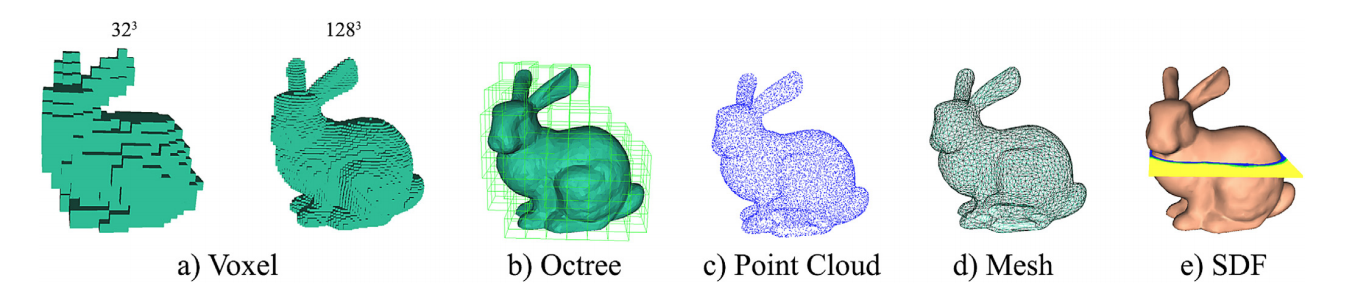
\includegraphics[width=1\textwidth]{images/3drepresentations.png}
        \caption{The Stanford Bunny in different 3D representations                     \cite{fahim2021single}
        .}
        \label{fig:3drepresentations}
\end{figure}

Moreover, RGB-D images contribute to this representation by storing a fourth channel, i.e. a depth map, alongside the 2D color information (RGB). Depth is the distance from the camera to the surface of objects in an image and it can be measured, for example, using time-of-flight sensors. These sensors measure the time in the signal from when the sensor was emitted to when the signal returned to the sensor, after being reflected by an object's surface. The most common types of signals used in these sensors are sound and light. Infrared light is usually preferred since it guarantees less noise and allows distinction from ambient light \cite{terabee2021tofprinciple}. In general, these devices have a limited depth of field, which limits the information captured from surfaces that are too close or too far away from the camera. Research on 3D information recovery from a scene has been extensively studied \cite{fahim2021single} for it is important for a wide range of applications, such as autonomous driving, industrial imaging, etc. Similarly, the amount of RGB-D datasets available online is massive in comparison to 3D datasets of labeled point clouds or meshes \cite{firman2016rgbd}. RGB-D image representations are therefore known as "2.5D" data \cite{ahmed2018survey}, since they are not actual 3D representations of objects and spaces. Accordingly, Representations of 3D data can be categorized into Euclidean and non-Euclidean (geometric) representations. Eucledian representations include voxels and octrees, and non-Eucledian representations include point clouds and meshes. Fig \ref{fig:3drepresentations} displays some of the possible representations of 3D data. 


\begin{figure}[!ht]
        \centering
        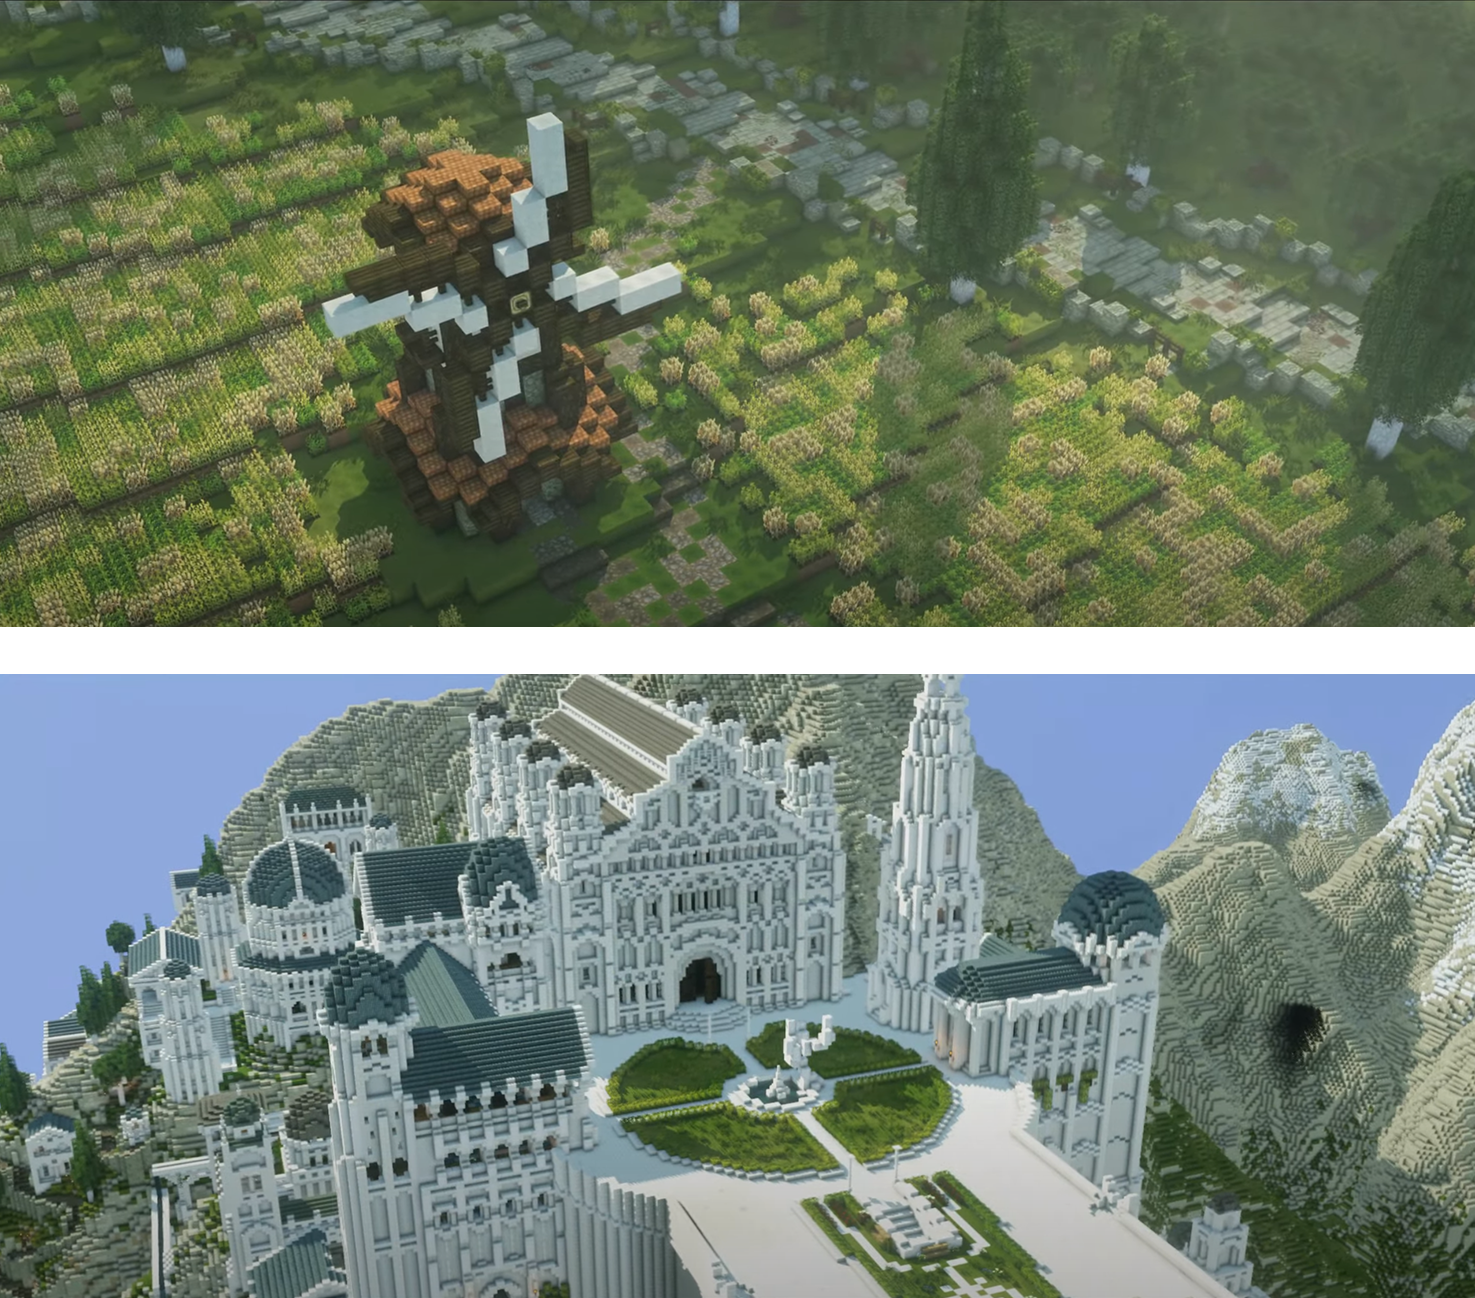
\includegraphics[width=0.7\textwidth]{images/minecraft.png}
        \caption{Voxelized representation of Minas Tirith in Minecraft \cite{minecraft2020minastirith}.\\A multitude of voxels can also represent high-resolution data, at a high computational memory cost (image below).
        }
        \label{fig:minecraft}
\end{figure}


This work focuses mainly on endeavors that work with voxel-based representations of 3D data. Similar to how 2D data can be represented in a 2D matrix, 3D data can be represented as a regular grid in the three-dimensional space \cite{ahmed2018survey}, where each cell or region contains information about the objects that are inside of it, if it is occupied or not, etc. These regions in a 3D grid are called voxels. Figure \ref{fig:minecraft} visualizes a video game called Minecraft, where the low resolution can be seen as voxels, even though the rendering engine used is not voxel-based. The main disadvantage of using voxels in high-resolution data is the amount of unnecessary memory storage required. However, one can leverage sparse voxel octrees (SVO) to down-sampling 3D scenes and navigate a simplified version of the environments. Accordingly, this thesis work leverages SVOs and low-resolution voxels (occupancy grids) to explore 3D simplified environments and and scan objects. The motivation for this is two-fold: first, as described by \cite{mcgraw2020high}, SVOs provide a huge reduction of memory requirements for most scenes, since empty space is not explicitly stored. Second, voxels describe the 3D structure of objects in a low-resolution fashion, and they can be used as extrinsic rewards to motivate a learning agent to explore thorough trajectories around objects. These trajectories then serve the purpose of exploring objects from multiple angles. % e biggest disadvantage is for rendering purposes, but this thesis uses
For further discussion on different representations of 3D data, one can refer to these outstanding surveys \cite{ahmed2018survey, ioannidou2017deep}. 


\begin{figure}[!ht]
        \centering
        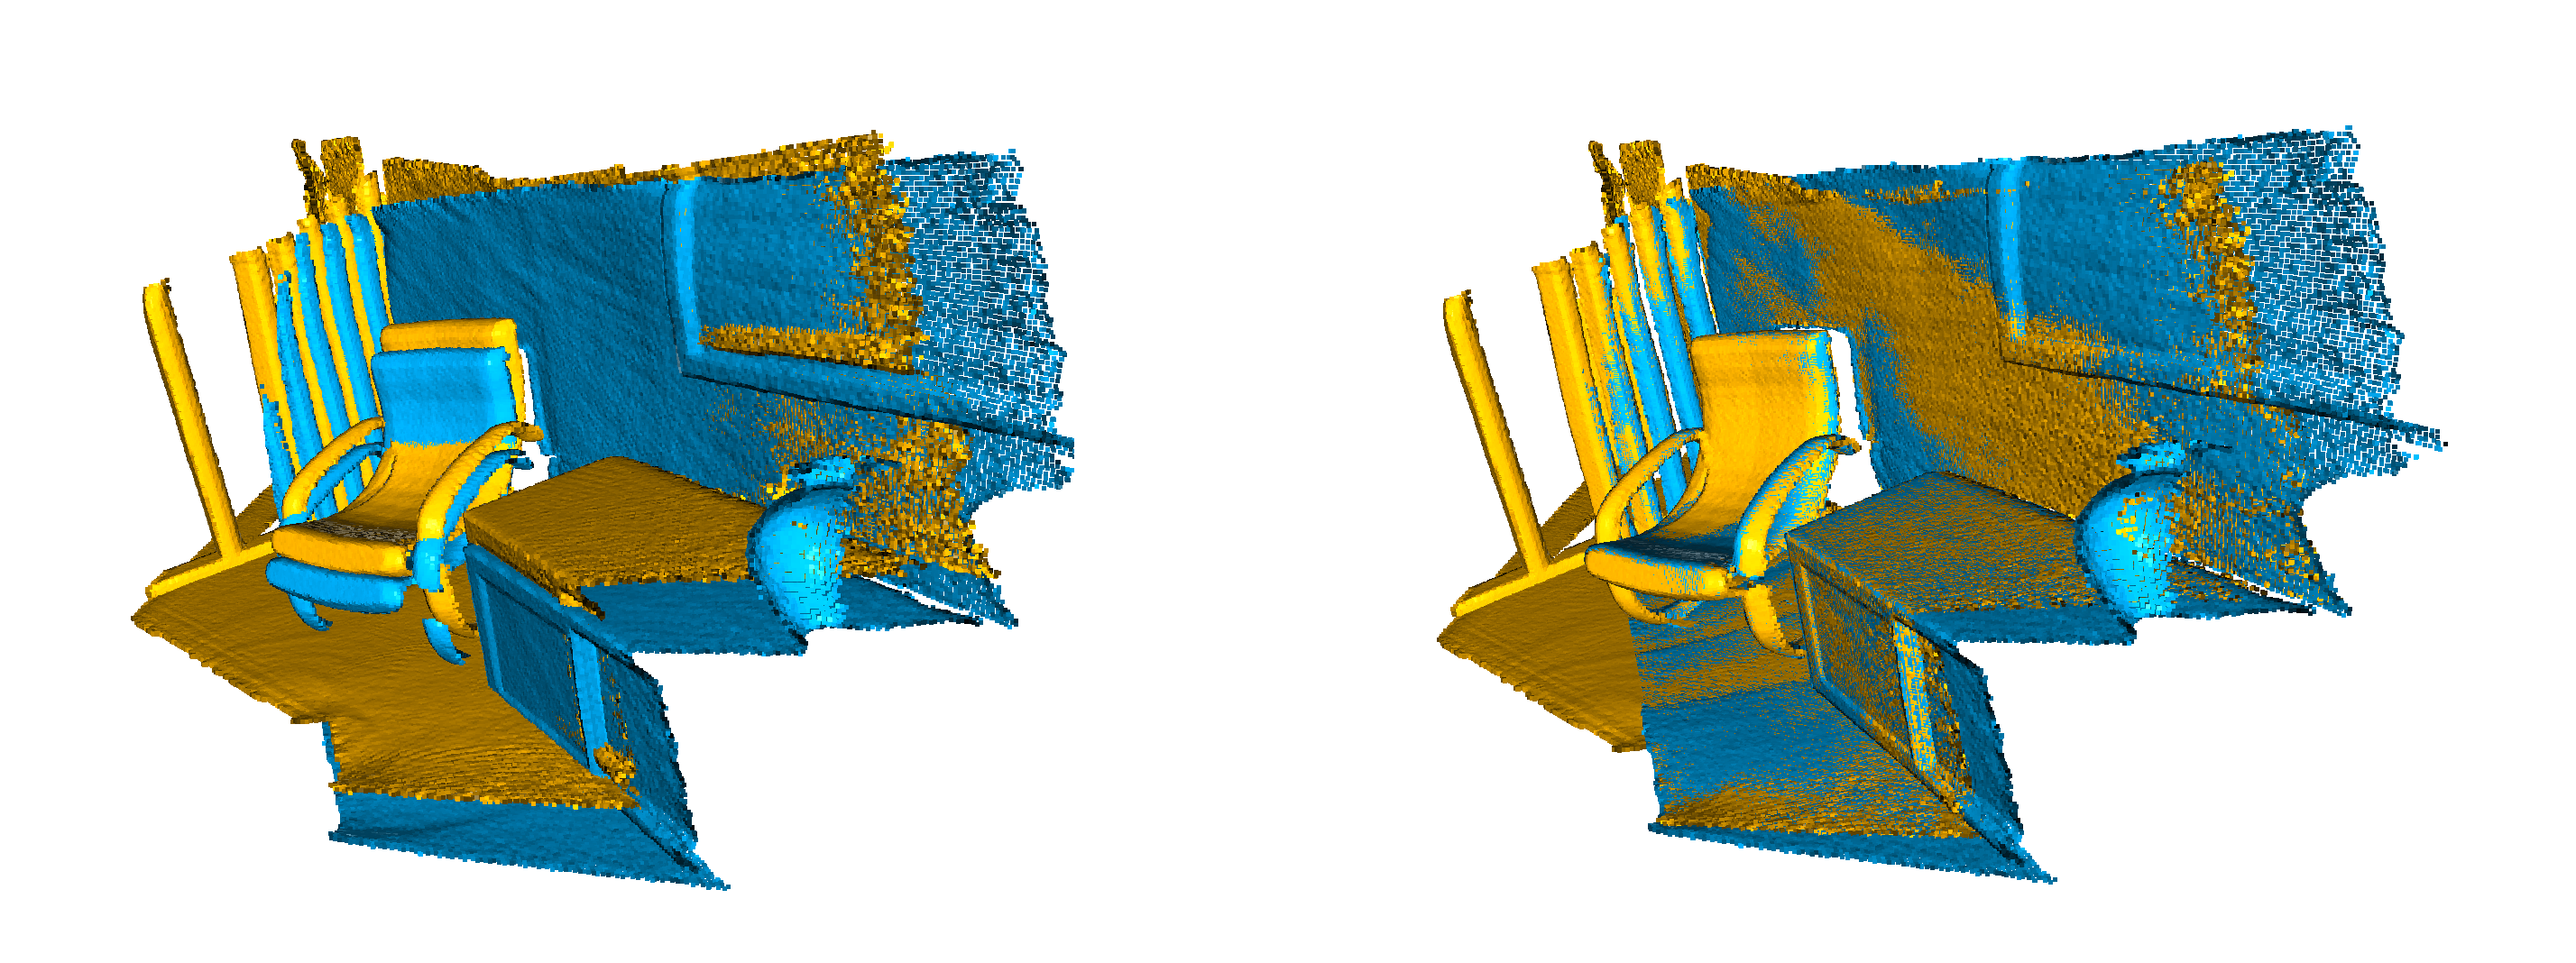
\includegraphics[width=0.8\textwidth]{images/icpalgorithm.png}
        \caption{Two input point clouds (left). Result after running the ICP Algorithm until convergence (right) \cite{open3D2021icp}.
        }
        \label{fig:icpalgorithm}
\end{figure}


Given an RGBD image, the process of generating a voxel grid from a triangle mesh is called voxelization \cite{open3D2021voxelization}. A voxel contains per default a "0" in the space it encloses. A "1" is assigned if the voxel is intersected with a triangle. However, one must obtain a point cloud beforehand from the RGBD data sent by a camera. Many works \cite{jia2019new, huang2021comprehensive} occupy themselves with point clouds from RGBD data, point cloud registration and the problem of outlier filtering when matching the RGB channel and the depth channel. Outlier filtering is required given that the alignment between the two channels can suffer from varying lighting conditions, reflective characteristics and particular sensor attributes. The further alignment in point cloud registration must also take into account a global world model when merging two point clouds together. Figure \ref{fig:icpalgorithm} displays the ICP algorithm \cite{open3D2021icp} for matching two point clouds together. Ultimately, a point cloud can then be voxelized or down-sampled to voxels for further processing \cite{open3D2021pointcloud}.


% Moreover, for a detailed pipeline on how to go from point clouds to voxels, see Appendix \ref{}



% \subsection{From Point Clouds to Voxels}\label{chap:2:pc-segmentation}
% This work aims to contribute to research on exploratory techniques using reinforcement learning.

% - what are images
% https://web.stanford.edu/class/cs101/image-1-introduction.html
% - what are DEPTH images
% http://cs231n.stanford.edu/reports/2016/pdfs/407_Report.pdf
% http://stanford.edu/class/ee367/Winter2020/report/lee_hong_lee_report.pdf

% - what are point clouds
% https://www.navvis.com/blog/everything-you-need-to-know-about-point-clouds-navvis


% - what are voxels
% https://en.wikipedia.org/wiki/Voxel
% % https://blog.spatial.com/the-main-benefits-and-disadvantages-of-voxel-modeling
% https://www.gamersnexus.net/gg/762-voxels-vs-vertexes-in-games

% \textbf{Limitations of Voxels.}

% \textbf{Applications of Voxels.}


\section{Octrees}\label{chap2:octrees}


\begin{figure}[!ht]
        \centering
        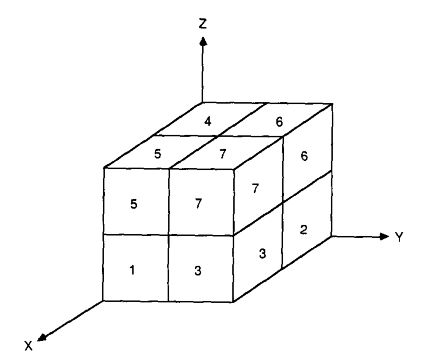
\includegraphics[width=0.4\textwidth]{images/octree.png}
        \caption{Labels of the octants of a cube (octant 0 is in the back and is not shown) \cite{chen1988survey}.
        }
        \label{fig:octree}
\end{figure}


% \textbf{Definition of Octrees. } 
The octree encoding uses a hierarchical tree data structure, where analog to quadtrees, each node can have up to eight children  \cite{meagher1980octree}. Octrees are used to model 3D spaces, since they allow the representation of a cubical region as shown in Figure \ref{fig:octree}. Whereas the root node represents the entire space, the rest of the octree is populated by the recursive subdivision of the 3D space into eight octants as shown in Figure \ref{fig:octree-vs-voxel}. Once the maximum resolution has been reached, nodes represent the leaves of the octree. Leaves in a node that have the same attributes can be reduced to a node by a process called condensation.
% ref here https://www.cg.tuwien.ac.at/studentwork/VisFoSe98/eder/octree.htm
Consequently, leaf nodes can be "point nodes" or "empty nodes", and a node that contains leaves is called a "region node".
% ref https://iq.opengenus.org/octree/\textbf

Information represented in leaves can be boolean or non-boolean if one decides to store more information in the tree such as temperature, etc. Condensation, however, is not a trivial process in non-boolean leaves. Finally, the implementation of octrees can be pointer-based or array-based. The pointer-based approach references child nodes as they are occupied by an object and are memory efficient. Array-based octrees define a priori all possible children in the hierarchy of the octree, making addressing of any node possible at the cost of memory.

 The resolution of the 3D space represented through an octree can be given as 2\textsuperscript{n}, and it is the octree's length space. The resulting volume enclosed by the octree consists of then $2\textsuperscript{n}\times2\textsuperscript{n}\times2\textsuperscript{n}$ octants. 
% Unit cubes can have values of 0 or 1 depending on the existence of objects inside of them.
% T
% When the maximum resolution is 
% There are different types of octrees, according to how the space is


% The octree space is usually modeled as a cubical region consisting of 2\^n x 2\^n x 2\^n 
% unit cubes, where n is the resolution parameter and 2\^n is the length of the octree 
% space. Each unit cube has value 0 or 1, depending on whether it is outside or inside
% the objects. 

% The octree representation of the objects is obtained by recursively
% subdividing the cubic space into octants.

% The results of the recursive subdivision process is represented by a tree of degree 
% 8 whose nodes are either leaves or have eight children. Thus, the tree is called an
% octree. Each node of the tree is given the same label as that assigned to its 
% corresponding o&ant. The root node of the resulting tree represents the entire space.

% Each node in an octree subdivides the space it represents into eight octants. 

% In a point region (PR) octree, the node stores an explicit three-dimensional point, which is the "center" of the subdivision for that node; the point defines one of the corners for each of the eight children. 
% In a matrix based (MX) octree, the subdivision point is implicitly the center of the space the node represents. 

% The root node of a PR octree can represent infinite space; 
% the root node of an MX octree must represent a finite bounded space so that the implicit centers are well-defined. 
% Note that Octrees are not the same as k-d trees: k-d trees split along a dimension and octrees split around a point. Also k-d trees are always binary, which is not the case for octrees.

% Less significant bits are sometimes ignored to reduce the tree size.
% The algorithm is highly memory efficient because the tree's size can be limited


% Three types of nodes are used in octree:

% Point node: Used to represent of a point. Is always a leaf node.
% Empty node: Used as a leaf node to represent that no point exists in the region it represent.
% Region node: This is always an internal node. It is used to represent a 3D region or a cuboid.


\begin{figure}[!ht]
        \centering
        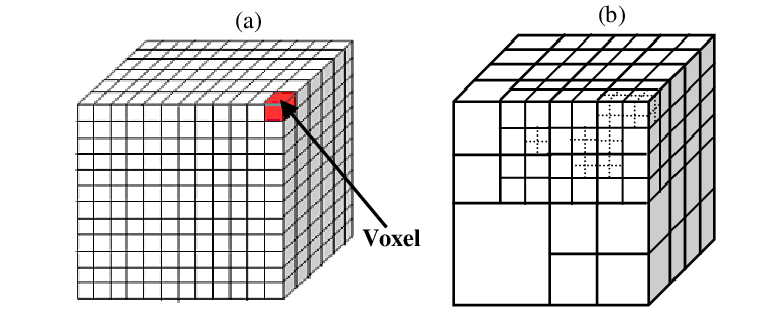
\includegraphics[width=0.7\textwidth]{images/voxelgridvsoctree.png}
        \caption{(a) Voxel grid (b) Octree representation \cite{saaidi2014multi}.
        }
        \label{fig:octree-vs-voxel}
\end{figure}


It is worth clarifying that the difference between a voxel grid and an octree is that a voxel grid is a fixed-resolution representation of 3D data, whereas the octree is multiresolution. When using in a rendering engine, octree rendering methods can load areas with higher resolution as one navigates the environment while keeping the other areas unloaded and preserving memory efficiency. A voxelgrid, in contrast, would always keep the same fixed resolution as one zooms in and out a render. Figure \ref{fig:octree-vs-voxel} aims to visualize the differences between an octree and a voxelgrid. For information on the complex manipulation of octrees and implementations of the search and insertion operations, please refer to \textcite{opengenus2021octree, geeksforgeeks2021octree}.
% https://iq.opengenus.org/octree/
% https://www.geeksforgeeks.org/octree-insertion-and-searching/

% \textbf{Sparse Voxel Octrees.}
% SVO is basically an octree, which holds only the mesh values (i.e. it is sparse) and only cubes (i.e. it is voxel, since general octree can hold points or triangles). I.e. SVO will hold only the visible cubes in minecraft, while all the invisible (not digged to yet) cubes are simply absent, resulting in a very efficient culling. Given that it is octree, we can use efficient O(log2(n)) search to check is that cube is visible to the player, compared to the usual grid raymarching, going over all the cells in line. Although the usual grid raymarching can still be speedup with signed distance field values inside empty grid cells. The O(log2(n)) per ray makes it fast enough for raycasting implementaton. But generally it used only as alternative to polygons, when you need to stream very detailed static models from the secondary storage or over the network, since animating voxel meshes is a very non-trivial subject, although it apparently can be done with signed distance fields, but it will be a bit slower than triangles. TLDR: SVOs are a way to render very large static meshes, that cant be fit into video memory and have to reside on disk drive to be preloaded on demand at the desired level of detail.

\textbf{Applications of Octrees.}
Octree's main application is using it as an acceleration structure given that memory and inference times increase cubically as the size of the 3D data increases. 
First, they excell as sparse data structures where empty regions consume little to no memory \cite{laine2010efficient}.
Second, in situations where meshes are too big for the available hardware, they allow efficient scaling through loading of 3D models at lower resolutions. 
Third, their efficient $O(log_{2}n)$ search queries when verifying the visibility of a cube make them an efficient data structure for high-quality ray casting of static scenes \cite{gobbetti2008single}.
Consequently, the efficient representation of high-resolution 3D models using octrees in comparison to polygon-based methods has been studied in a multitude of works such as fast collision detection in models of over 25M polygons \cite{melero2019fast}, solar radiation \cite{liang2017sparse}, voxelized full-waveform airborne LIDAR data \cite{miltiadou2021comparative}, volume rendering methods \cite{knoll2006survey}, adaptive resolution SLAM \cite{vespa2019adaptive}, etc. In terms of limitations, octree-based techniques are not straight-forward since octrees are difficult to implement and manipulate. Moreover, operations on octrees in dynamic scenes where nodes need to be continuously recalculated are not efficient. This thesis limits itself to the usage of sparse boolean octrees as a mapping structure for a 3D scene where newly discovered nodes provide an intrinsic reward to the agent. Hence, the limitations of octrees are disregarded.



% Octree ray casting/tracing is just the act of raytacing, but using an octree as an acceleration structure rather than nothing or a uniform grid (like how traditional voxels are stored).
% Some advantages of using an octree is that A) ray collision queries can be accelerated by them, and B) octrees, and particularly sparse octrees, can make empty/air regions consume little or no storage.

% if your game uses raytracing, the graphics performance would be better using this data structure. In addition, octrees can reduce the memory footprint of large voxel scenes when there are lots of empty areas.
% https://www.reddit.com/r/VoxelGameDev/comments/ioe7wc/advantages_of_advanced_voxel_rendering_techniques/
% Advantages:
% Can represent crazy amount of detail as voxels that would be impossible with a polygon engine. With polygons, you need to LOD aggressively to keep things managable, here you can show intricate detail quite far away.
% Many basic rendering effects are very simple. You can have high quality shadows on everything with just a few lines of code, whereas managing shadow maps for polygon rendering efficiently is really hard.
% Modifying the world during gameplay probably easier than with polygons.
% Modern hardware is ready for it. I can render basic worlds represented with 36 trillion voxels at 4K in 60fps.. on a 1080Ti.
% Easy to scale. Doesn't run fast enough? render natively at a lower res.
% You get a "unique look" for your game, for free. Good to have nowadays.

% \textbf{Limitations of Octrees.}


% An obvious con of using this is that it can be harder to code than more basic solutions. There are likely other cons, but I don't want to speak outside my realm of knowledge here.

% I don't know which paper is "optimal", but I would search on Google scholar "efficient sparse voxel octrees" and look at some of the papers. Their implementation is brutal I hear, but the papers explain what is happening.

% Disadvantages:

% Though you do not strictly need LOD, dealing with aliasing effects if you don't do LOD. So you'll want the ray to stop at a certain size voxel. Use TAA if you can, its best at fixing the typical aliasing you get from ray-tracing.

% It's hard to efficiently have some rendering effects for some surfaces and not others. Your renderer works better the more uniform it is.

% Every extra ray costs a lot. I do a primary ray and a shadow ray, and a reflection ray would slow things down quite a bit.

% Not easy to do dynamic or animated objects. Again, everything has to be part of the same ray-cast to be efficient, so fastest would be to have your moving objects be part of the world structure somehow. Making them free-floating means you have to trace the world octree AND a model AABB tree or something for every ray, probably cutting your performance in half or worse. Or you could render models using polygons, and have them look funny when models and the world don't shadow each other correctly etc.

% Probably not great still on low end laptops or mobile hardware, even with the res scaled way down.

% You best enjoy writing your own rendering engines because EVERYTHING is going to be custom, and different from existing engines.

%  going into the 3d world
% point cloud segmentation, point cloud registration, scene understanding, and reinforcement learning 
\section{Scene Understanding}\label{chap2:scene-understanding}
% \lipsum[1-3]
% the same way that iphones rose, smart robots will rise.
% As algorithms and technologies continue to improve over the years, we have witnessed the rise of smartphones, smart homes and now smart offices. 

In their 2020 Hype Cycle for Artificial Intelligence, Gartner projects smart robots to be at their peak of expectations in about 2 to 5 years. This projection goes hand-in-hand with another projection in the same hype cycle. Gartner projects that computer vision will be on the slope of enlightenment around the same period. This is where the experts predict computer vision will enable applications to exploit another input stream: vision. The same way that computers and embedded systems are able to interpret audio and text input from sensors, keyboards, microphones, etc., systems will have access to vision to perform a variety of tasks. 
% n will enable systems to leverage vision for a variety of tasks. 
As \textcite{singh2018fotonnet} describes, "the ability for robots and computers to see and understand the environment is becoming a burgeoning field, needed in autonomous vehicles, augmented reality, drones, facial recognition, and robotic helpers". Since the rise of the CNN \cite{krizhevsky2017imagenet} deep learning based methods for image classification have reached state of the art performance for 2D detection.
% Object localization and segmentation are extensions to the image classification problem, which .
% which current 2D methods can now tackle. 

% In this work the focus is one of the current challenges for computer vision: 3D object recognition. As of today

% available 2D information, new geometric features, etc. 
% Even though 3D labeled data sets are scarce \cite{singh}, this is slowly changing \cite{google}\cite{3ddataset}. Likewise, 3D-depth sensors are not widely available as of today \ref{singh}, but this is slowly changing \ref{cheap-3d-sensors-phone}. 
% to 3D-image sensors in phone 
% due to the growing availability of public large data sets. low-cost 3D image sensors,  in the development phase, due in great part to a lack of publicly available large data sets. 

% \textbf{Definition of Scene Understanding.}
\begin{figure}[!ht]
        \centering
        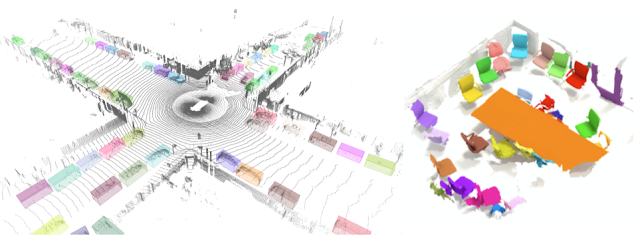
\includegraphics[width=0.9\textwidth]{images/sceneU01.png}
        \caption{3D object detection (left) and 3D instance segmentation (right) using Tensorflow 3D as found in \cite{najibi2020dops}.
        }
        \label{fig:sceneU01}
\end{figure}


The visible growth over the past few years of 3D sensors in our day-to-day surroundings (LIDAR, depth cameras, radar) comes hand-in-hand with the requirement for efficient and accurate machine-learning-powered scene understanding methods that can process the data coming from these sensors. Suitable example applications are self-driving cars and robots where they need a sense of embodiment to interpret their environments and navigate around them or augmented reality experiences. Consequently, even though research in computer vision has been recently pushing the state-of-the-art techniques in 3D object detection, much remains to be done to improve the workflow and research of techniques using 3D data. Libraries like Tensorflow3D \cite{najibi2020dops}, Pytorch3D \cite{ravi2020pytorch3d}, Torch-Points3D \cite{tp3d}, Pytorch Geometric \cite{Fey/Lenssen/2019}, etc., aim to make deep learning models and dataset processing tools available to developers and researchers. Some of the main research areas include: 3D semantic segmentation, 3D object shape prediction, point cloud registration and point cloud densification.

% This is a framework for running common deep learning models for point cloud analysis tasks against classic benchmark. It heavily relies on Pytorch Geometric and Facebook Hydra.

% The framework allows lean and yet complex model to be built with minimum effort and great reproducibility. It also provide a high level API to democratize deep learning on pointclouds. See our paper at 3DV for an overview of the framework capacities and benchmarks of state-of-the-art networks.



% https://ai.googleblog.com/2021/02/3d-scene-understanding-with-tensorflow.html
% add picture from TF
Given the inherent sparse nature of 3D data in our surroundings, denoted as open space, appropriate data structures and algorithms for efficient memory and inference operations are required. Accordingly, sparse convolutional models with pooling operations are seen in the core backbones of most state-of-the-art methods used in outdoor autonomous driving and indoor benchmarks, such as Waymo, NuScenes and ScanNet \cite{najibi2020dops}.
Tensorflow, for example, uses the 3D submanifold sparse U-net architecture to extract both coarse and fine features from voxels. This network, as shown in Figure \ref{fig:u-net}, consists of three components: an encoder, a bottleneck and a decoder. A set of prediction heads can then be added according to the task at hand. Implementations involving sparse convolutions combined with CUDA techniques show improvements of up to 20x with respect to previous implementations \cite{najibi2020dops}.

% \begin{figure}[!ht]
%         \centering
%         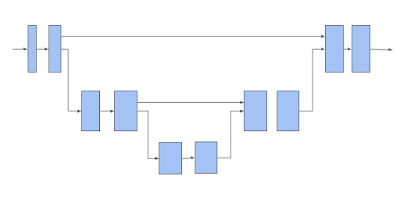
\includegraphics[width=0.65\textwidth]{images/u-net.png}
%         \caption{ A 3D sparse voxel U-Net architecture using submanifold sparse convolutions (horizontal arrows) and submanifold sparse pooling (arrows downward) operations \cite{tf}.
%         }
%         \label{fig:u-net}
% \end{figure}


% make a couple sentences
% 3D Sparse Convolutional Network
% The 3D data captured by sensors often consists of a scene that contains a set of objects of interest (e.g. cars, pedestrians, etc.) surrounded mostly by open space, which is of limited (or no) interest. As such, 3D data is inherently sparse.

% Sparse convolutional models are core to the state-of-the-art methods applied in most outdoor self-driving (e.g. Waymo, NuScenes) and indoor benchmarks (e.g. ScanNet).In such an environment, standard implementation of convolutions would be computationally intensive and consume a large amount of memory. 

% So, in TF 3D we use submanifold sparse convolution and pooling operations, which are designed to process 3D sparse data more efficiently. 

% We also use various CUDA techniques to speed up Experiments on the Waymo Open dataset shows that this implementation is around 20x faster than a well-designed implementation with pre-existing TensorFlow operations.

% TF 3D then uses the 3D submanifold sparse U-Net architecture to extract a feature for each voxel. The U-Net architecture has proven to be effective by letting the network extract both coarse and fine features and combining them to make the predictions.
% The U-Net network consists of three modules, an encoder, a bottleneck, and a decoder, each of which consists of a number of sparse convolution blocks with possible pooling or un-pooling operations.


% A 3D sparse voxel U-Net architecture. Note that a horizontal arrow takes in the voxel features and applies a submanifold sparse convolution to it. An arrow that is moving down performs a submanifold sparse pooling. An arrow that is moving up will gather back the pooled features, concatenate them with the features coming from the horizontal arrow, and perform a submanifold sparse convolution on the concatenated features.


% The sparse convolutional network described above is the backbone for the 3D scene understanding pipelines that are offered in TF 3D. Each of the models described below uses this backbone network to extract features for the sparse voxels, and then adds one or multiple additional prediction heads to infer the task of interest. 
% The user can configure the U-Net network by changing the number of encoder / decoder layers and the number of convolutions in each layer, and by modifying the convolution filter sizes, which enables a wide range of speed / accuracy tradeoffs to be explored through the different backbone configurations

% discussion future work, add photo of encoder
% In our recent paper, “DOPS: Learning to Detect 3D Objects and Predict their 3D Shapes”, we describe in detail the single-stage weakly supervised learning algorithm used for object detection in TF 3D. In addition, in a follow up work, we extended the 3D object detection model to leverage temporal information by proposing a sparse LSTM-based multi-frame model. We go on to show that this temporal model outperforms the frame-by-frame approach by 7.5% in the Waymo Open dataset.


\textbf{Applications of 3D Scene Understanding.}
Scene understanding techniques have been seen in a multitude of tasks, such as: rendering textured meshes or point clouds, camera position estimation, fitting meshes with textures, pose estimation, point cloud completion, and point cloud registration \cite{najibi2020dops, ravi2020pytorch3d}. A great effort has gone particularly into:
\begin{itemize}
    \item Semantic segmentation, where models predict per-voxel semantic scores using one output head, which are then mapped and used to label 3D points \cite{najibi2020dops, hackel2017semantic3d, qi2017pointnet, qi2017pointnet++}.
    \item Instance segmentation, where models group voxels that belong to the same object together using a per-voxel instance embedding vector and then predict a semantic score per-voxel. When the input consists of a point cloud instead of an image, methods using sparse 3D convolutions are preferred \cite{najibi2020dops, jiang2020pointgroup}.
    \item Object detection, where models uses box prediction and classification losses to predict per-voxel semantic scores, size, rotation matrices, and center, which are then reduced to accurate box proposals during inference time \cite{najibi2020dops, qi2019deep}. 
\end{itemize}

\textbf{Limitations of 3D Scene Understanding.}
% Scene Understanding Using Deep Neural Networks—Objects, Actions, and Events: A Review
As documented by \textcite{surendran2020scene}, the major drawbacks of current deep learning techniques include computational complexity and execution speed particular to each technique. Nevertheless, attaining high accuracy is one of the core challenges, especially in terms of distinguishing similar categories (selectivity) and in terms of robustness to rotations, scaling, translations and illumination changes (invariance).
One of the main causes for these symptoms in scene understanding research is the limited amount of publicly available 3D data sets \cite{han2019image}.
Research \cite{hackel2017semantic3d} highlights that the lack of rich 3D datasets is a major challenge in scene understanding research. For example, the Oakland dataset consists of less than 2 million labelled points, the NYU benchmark contains only indoor scenes and other data sets created using a 3D Velodyne LIDAR provide low point density meshes than those using a static scanner.
Another cause consists of the lack of accessibility for developers to hardware \cite{singh2018fotonnet} for 3D workflows. 

\begin{figure}[!ht]
        \centering
        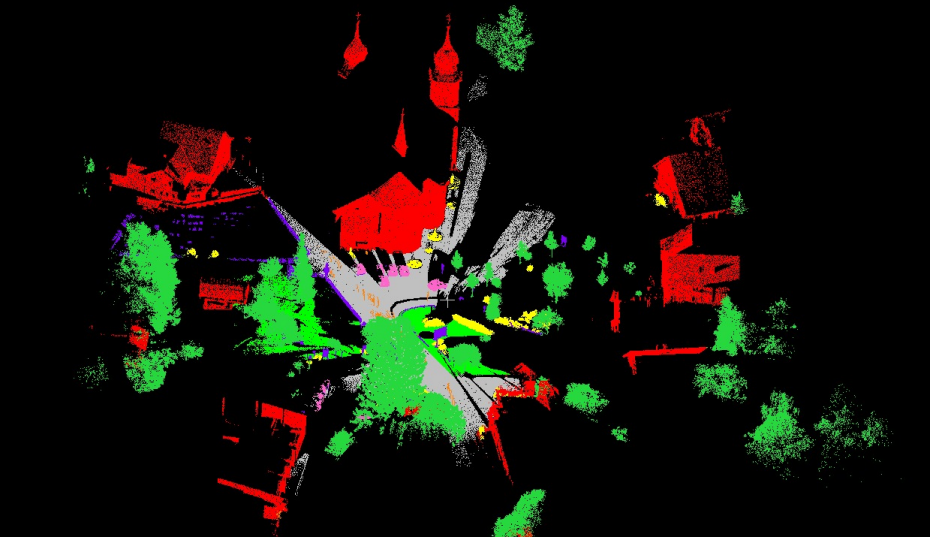
\includegraphics[width=0.7\textwidth]{images/sceneU02-hackel.png}
        \caption{Class labels example of Semantic3D \cite{hackel2017semantic3d}.
        }
        \label{fig:3Dsegsem-hackel}
\end{figure}


These two delaying factors are fortunately slowly changing: RGB-D data sets continue to be released to support the development of new algorithms. For example, the work by \textcite{hackel2017semantic3d} from ETH aids to the limited datasets problem by contributing with Semantic3D, the largest known labelled 3D point cloud data set of natural scenes, containing over 4 billion points. Another example is the MediaPipe data set released by Google in November of 2020 \cite{objectron2021dataset}. Moreover, accessibility to low-cost 3D sensors continues to increase: the newest smartphones, for example, are equipped with time-of-flight cameras, not only for photography but also extend their capabilities for AR applications and gaming \cite{tian2019occlusion}. Even though it is still not possible for any RGB-D data set to be as big as the ImageNet data set (∼5 million images), techniques continue to be developed to exploit geometric features and to utilize tools and concepts from 2D methods for 3D visual interpretation.

This thesis is motivated by the limitations present in the scene understanding field, and describes the promise of synthetic data in the following sections, which is then later exploited in the approach described in Chapter \ref{chap:3:title}. Similarly, given the limited amount of time and the extensive library of 3D methods, this work is constrained to 2D object detectors to define the concept of temporal uncertainty in a 3D scene, explained in the same chapter.
For more information on 2D object detectors, please refer to Appendix \ref{appendix:DL-for-vision}.

% https://ai.googleblog.com/2021/02/3d-scene-understanding-with-tensorflow.html
%  make one bullet point of each
% 3D Semantic Segmentation
% The 3D semantic segmentation model has only one output head for predicting the per-voxel semantic 

% 3D Instance Segmentation
% In 3D instance segmentation, in addition to predicting semantics, the goal is to group the voxels that belong to the same object together. The 3D instance segmentation algorithm used in TF 3D is based on our previous work on 2D image segmentation using deep metric learning. The model predicts a per-voxel instance embedding vector as well as a semantic score for each voxel. The instance embedding vectors map the voxels to an embedding space where voxels that correspond to the same object instance are close together, while those that correspond to different objects are far apart. In this case, the input is a point cloud instead of an image, and it uses a 3D sparse network instead of a 2D image network. At inference time, a greedy algorithm picks one instance seed at a time, and uses the distance between the voxel embeddings to group them into segments.

% 3D Object Detection
% The 3D object detection model predicts per-voxel size, center, and rotation matrices and the object semantic scores. At inference time, a box proposal mechanism is used to reduce the hundreds of thousands of per-voxel box predictions into a few accurate box proposals, and then at training time, box prediction and classification losses are applied to per-voxel predictions.
% We apply a Huber loss on the distance between predicted and the ground-truth box corners. 
% Since the function that estimates the box corners from its size, center and rotation matrix is differentiable, the loss will automatically propagate back to those predicted object properties. 3
% We use a dynamic box classification loss that classifies a box that strongly overlaps with the ground-truth as positive and classifies the non-overlapping boxes as negative.


% https://prs.igp.ethz.ch/research/current_projects/3D_scene_understanding.html

% 3D point cloud classification is an important task with applications in robotics, augmented reality and urban planning.
% Recent advances in Machine Learning and Computer Vision have proven that complex real-​world tasks require large training data sets for classifier training. 
% At the same time, until now there were no data sets for 3D point cloud classification which would be sufficiently rich in both object representations and number of labelled points. For example, the well-​known Oakland data set contains less than 2 million labelled points. Another popular data set, the NYU benchmark, provides only indoor scenes. Finally, both Sydney Urban Objects data set and the IQmulus & TerraMobilita Contest use a 3D Velodyne LIDAR mounted on a car which provides much lower point density than a static scanner. The same counts for the Vaihingen3D airborne benchmark.

% This benchmark closes the gap and provides the largest known labelled 3D point cloud data set of natural scenes with over 3 billion points in total. It also covers a range of diverse urban scenes: churches, streets, railroad tracks, squares, villages, soccer fields, castles to name just a few. The point clouds we provide are scanned statically with state-​of-the-art equipment and contain very fine details. Our goal is to help data-​demanding methods like deep neural nets to unleash their full power and to learn richer 3D representations than it was ever possible before.

% https://ai.googleblog.com/2021/02/3d-scene-understanding-with-tensorflow.html
% https://prs.igp.ethz.ch/research/current_projects/3D_scene_understanding.html
% https://arxiv.org/pdf/2103.06422.pdf
% https://ethz.ch/content/dam/ethz/special-interest/baug/igp/photogrammetry-remote-sensing-dam/documents/pdf/wojek12.pdf

% Along these lines, research from 2020, such as PointContrast \cite{xie2020pointcontrast} and OcCo \cite{wang2020pre} propose pre-training on ShapeNet \cite{chang2015shapenet} to leverage the information contained in point clouds for scene understanding and for reconstructing occluded point clouds respectively. Figure \ref{fig:occo-results} illustrates the performance of OcCo pre-training  for completion of occluded point clouds.

% - some relevant works on PC
% https://prs.igp.ethz.ch/research/current_projects/registration-of-3dpoint-clouds-with-low-overlap.html
% https://prs.igp.ethz.ch/research/current_projects/geometric-deep-learning-for-point-cloud-processing.html
% https://ethz.ch/content/dam/ethz/special-interest/baug/igp/photogrammetry-remote-sensing-dam/documents/pdf/timo-jan-isprs2016.pdf

% \subsection{Understanding from Monocular Cameras}\label{chap:2:aa}


% \textbf{Monocular Videos.}
% Panoramic Visual SLAM Technology for Spherical Images


% 
% Its architecture also allows to keep the global context of the image at test time.  
\section{Defining Visual Uncertainty}\label{chap:2:semantic-entropy}






% new
\section{3D Environments}\label{chap2:3denvironment}

\begin{figure}[!ht]
    \centering
    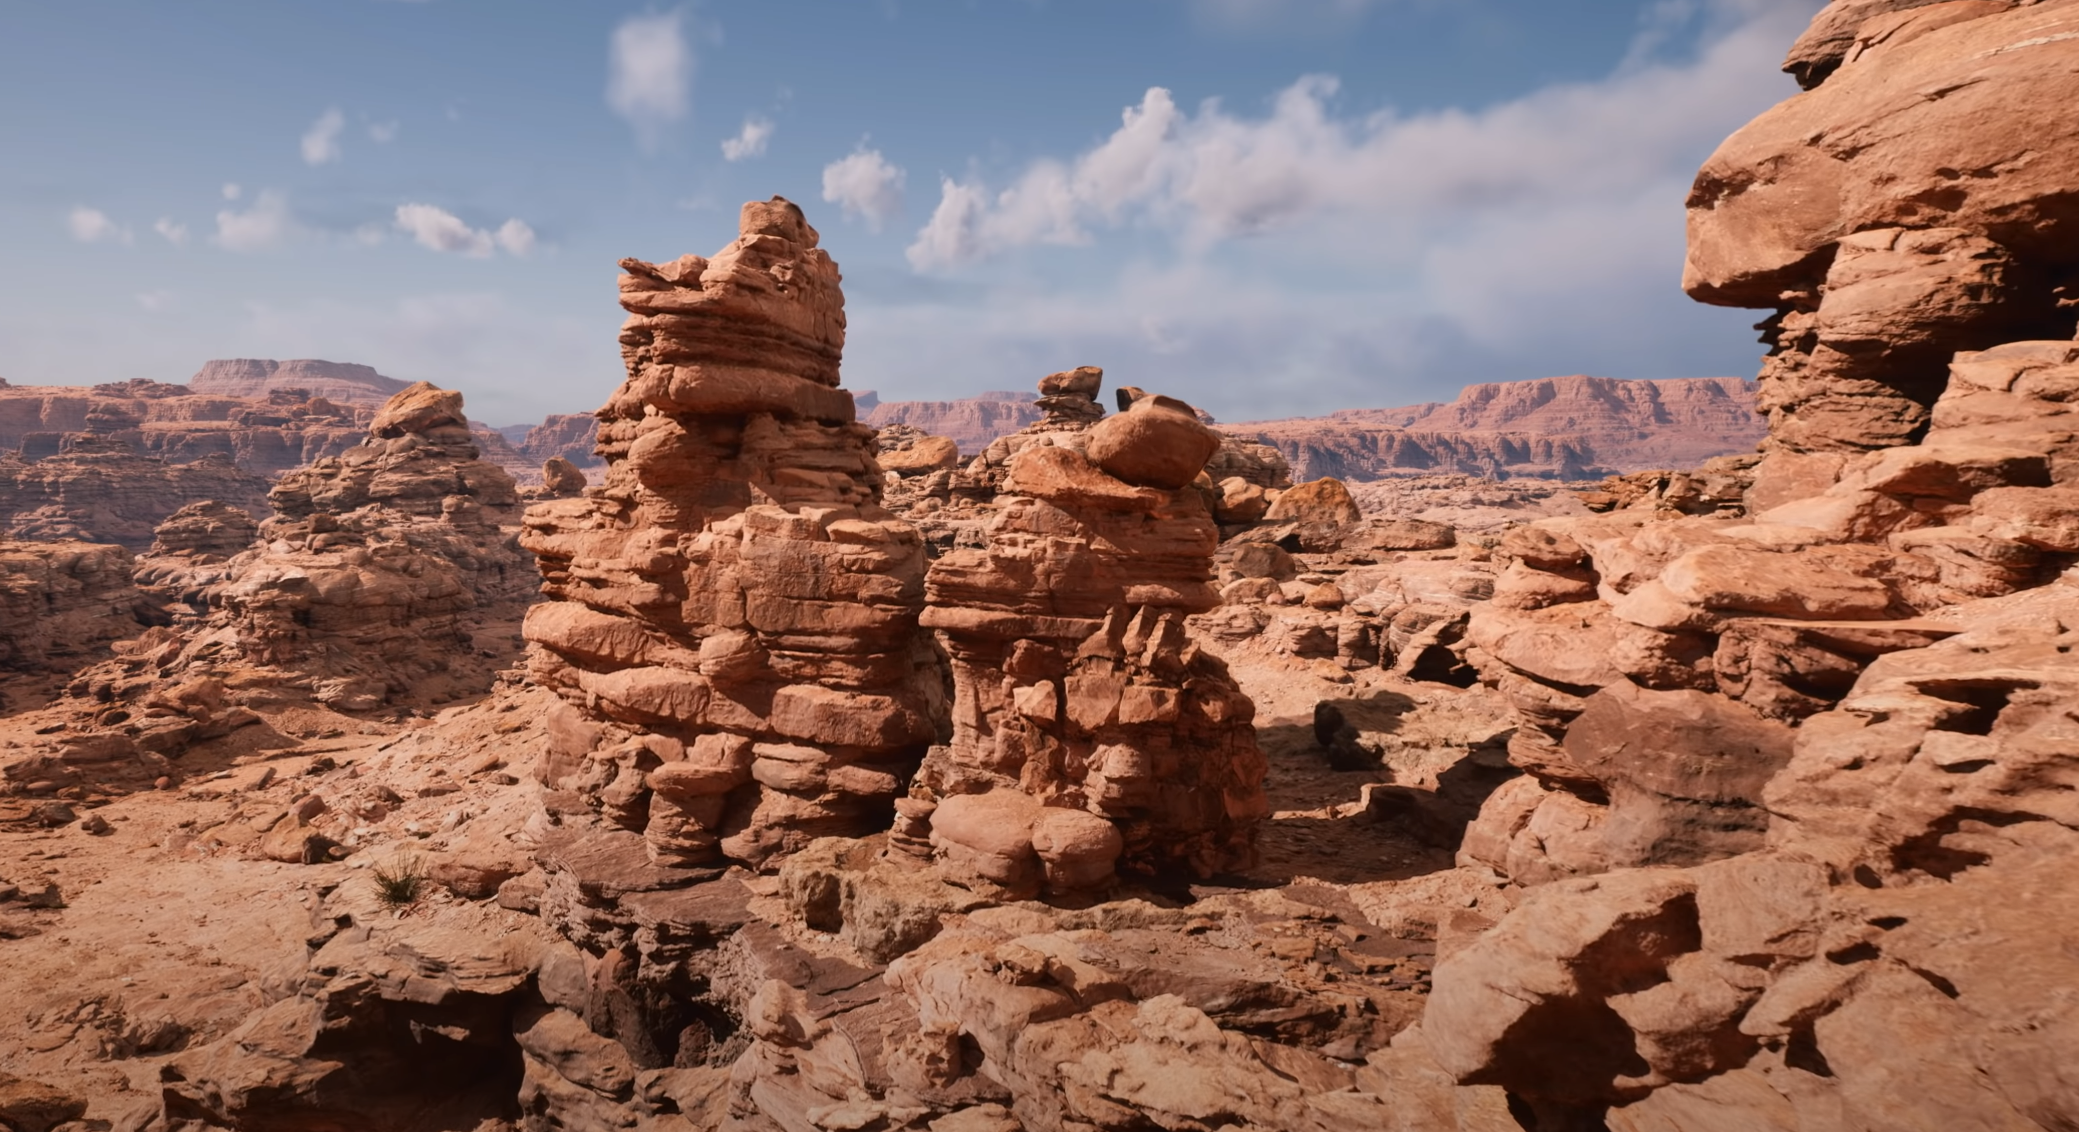
\includegraphics[width=0.7\textwidth]{images/unreal-desert2.png}
    \caption{3D hyper-realistic simulated desert using Unreal Engine 5 (early access) \cite{unreal5_2021}.}
    \label{fig:unreal-desert}
\end{figure}
    
    
Current software allows the creative development of simulated 3D environments, which can be executed and visualized on a variety of platforms, such as smartphones, gaming consoles, etc. 
% These 3D environments 
% https://spatial.io/
It is remarkable how the applications of simulated hyperrealistic environments continue to grow every year in architectural renderings, advertisements of specialized computer software, video games, movies, video calls \cite{spatial-io2021}, etc.
% overall creating a more immersive experience across all domains, where realism in 3D modeling software and game engines continues to improve.
The advent of 3D computer graphics, GPUs, rendering engines and techniques, and game engines continue to allow developers to come up with more sophisticated world simulations.
Life-like simulations are therefore possible through 3D environment modeling \cite{asma_2021}, which involves steps such as:
% source https://it-s.com/what-is-a-3d-modeled-environment/
\begin{enumerate}
    \item \textbf{Detailed concept development} of blueprints and insight of state-of-the-art art techniques
    \item \textbf{High-definition sketching} based on the predefined concepts 
    \item \textbf{Environment assets creation} of the objects that will be in the scene
    \item \textbf{Hyper-focused texturing} of the given objects, where natural textures must be applied to allow realism under different perspectives and lighting conditions.
    \item \textbf{High/Low-Poly modeling} depending on the purpose of the project and hardware constraints for rendering (real-time factor).
    \item \textbf{3D rendering and optimization} of parameters and light settings.
\end{enumerate}

The following sections give a brief overview of what game engines are and how they enable the creation of synthetic data for machine learning models.

\subsection{Game Engines and Simulation Environments}\label{chap2:gameengines}
Game Engines, like integrated development environments (IDEs), are software frameworks that allow the development of video games and 3D environments by providing an abstraction layer over a multitude of functionalities. They consist of a main game program, a rendering engine, an audio engine, a physics engine, and an artificial intelligence module, which take care of the following: 
\begin{itemize}
    \item \textbf{Input} from a multitude of devices such as keyboards, mice, screens, etc. This input can be obtained through polling or event-based mechanisms (i.e., obtaining the position of a cursor is polling-based and detecting a click from a mouse is event-based).
    \item \textbf{Graphics} which are generated by converting the geometric and color information of a scene from the virtual space of the application into a picture. This requires the usage of 3D assets, which are usually created using 3D modeling software such as Blender, Autodesk 3ds Max, Maya, etc. 
    \item \textbf{Physics}, where the laws of gravity, friction, and collision for the movement of a virtual object are simulated.
    \item \textbf{Artificial Intelligence} to give the characters in the environment a personality, such as animals, etc.
    \item \textbf{Sound} to represent sound effects, dialogue, music, etc. 
    \item \textbf{Networking} to abstract TCP/UDP and API integrations in the development of multiplayer games.
\end{itemize}

Physics simulators are an important part of robotics research, as they provide an environment for researchers to test and evaluate algorithms and/or architectures without the constraints and real-world complexity of the physical environment, including the physical degradation of robots. When simulating robots, one of the first questions we need to ask is what level of complexity we are willing to tackle, and where the simulations are going to be used. Moreover, simulations can run faster than real time, are parallelisable, and allow the environment to be reset or modified without physical effort. Finally, simulations are able to produce different sensory inputs which can be extremely valuable for robotics research.

\textcite{collins2021review} define a robotics simulator as an end-user software application that contains a realistic physics engine, collision and friction detection, GUI, supports 3D assets, allows a scripting mechanism, and can model robotic joints and actuators. Relevant game engines and simulation environments that can be used in the development of machine learning or robotic applications include: Unity 3D \cite{unity2021}, Unreal Engine \cite{unreal5_2021}, MuJoCo \cite{mujoco}, Gazebo Simulator \cite{osrf2021gazebosim} and CARLA \cite{Dosovitskiy17}.
% An overview of these frameworks is described below.
% \textbf{Unity 3D.}\label{chap:2:unity}
\textcite{collins2021review} provide an in-depth review of physics simulators for robotics applications with extensive comparative tables that set one simulator apart from other for each use case. Factors taken into account in the evaluation of the simulators include: fidelity of rigid or soft body contact dynamics, locomotion over irregular terrain, support for torque and vision sensors, noise simulation in sensors to approximate real world policies, domain randomization to diversify training data, texture randomization, randomization of object mass, inertia, and friction coefficients, support for multiple physics engines, support for parallel simulation, support for headless mode and rapid dynamic solvers, support for CPU and GPU optimizations.
% \begin{itemize}
%     \item Fidelity of rigid or soft body contact dynamics.
%     \item Locomotion over irregular terrain.
%     \item Support for torque and vision sensors, among others.
%     \item Noise simulation in sensors to approximate real world policies.
%     \item Domain randomization to diversify training data.
%     \item Texture randomization.
%     \item Randomization of object mass, inertia, and friction coefficients.
%     \item Support for multiple physics engines.
%     \item Support for parallel simulation.
%     \item Support for headless mode and rapid dynamic solvers.
%     \item Support for CPU and GPU optimizations.
% \end{itemize}

\begin{figure}[!ht]
    \centering
    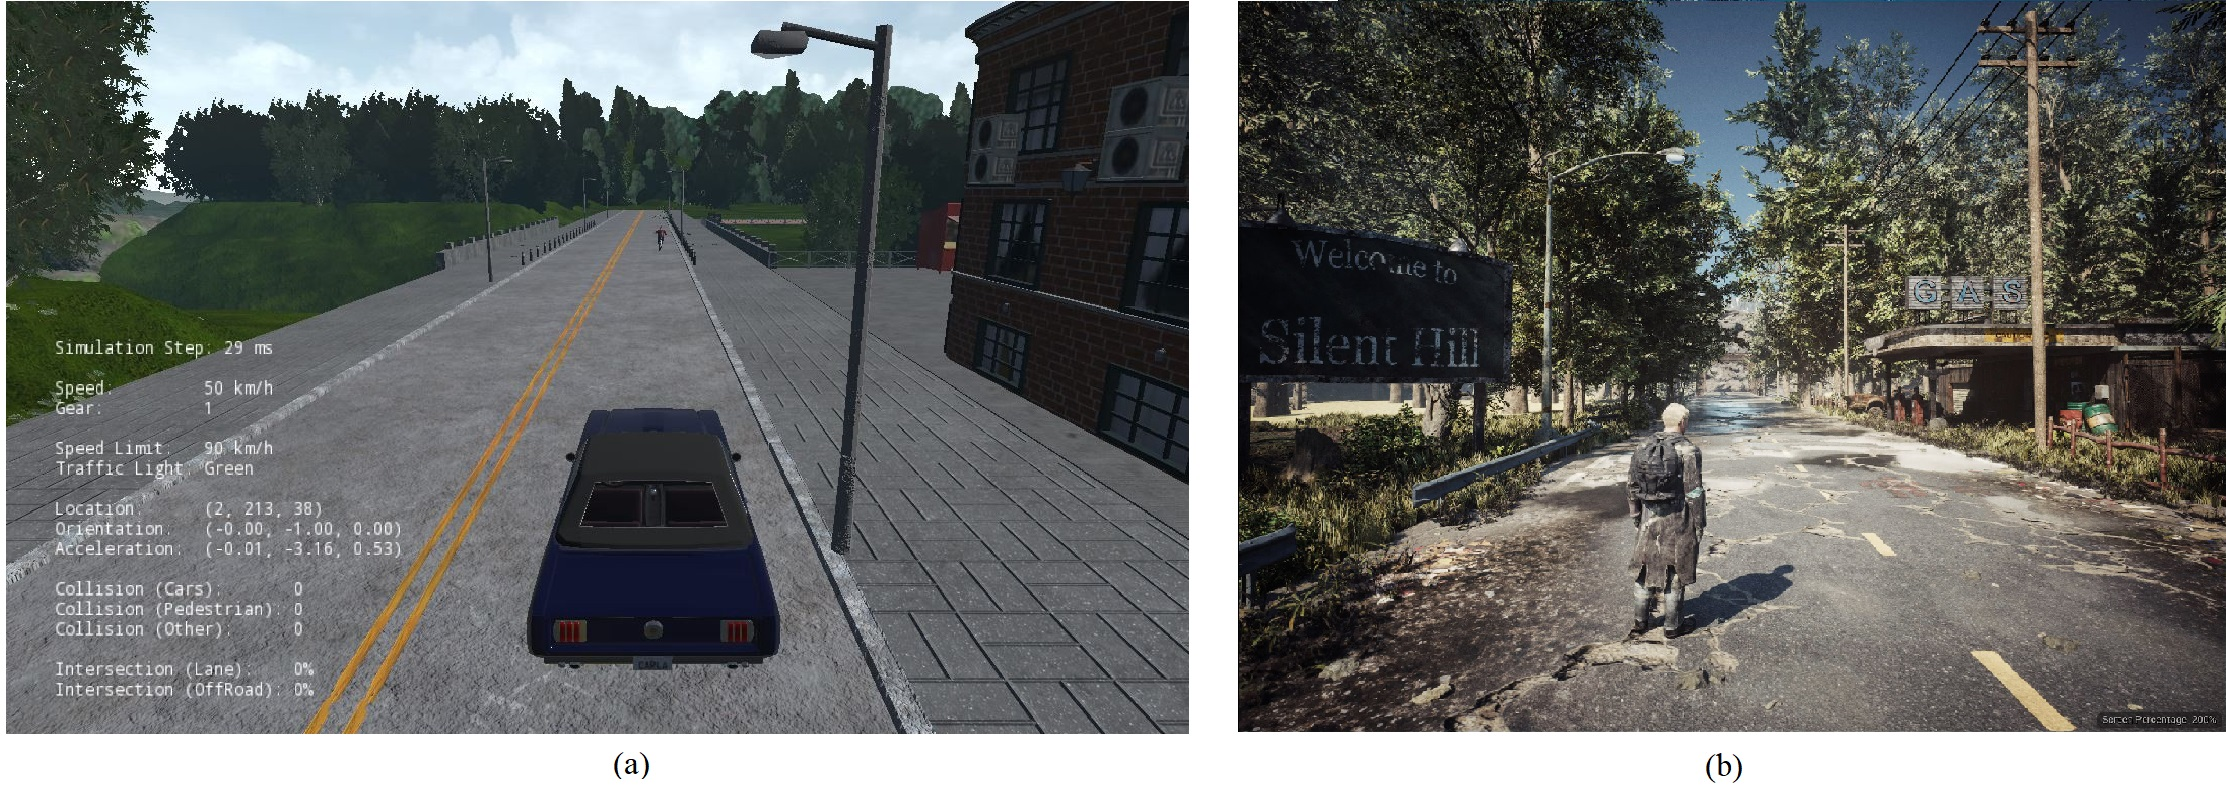
\includegraphics[width=0.95\textwidth]{images/carla-vs-unreal.jpg}
    \caption{Comparison of the capabilities between two simulators of creating realistic 3D environments: (a) CARLA \cite{Dosovitskiy17}, (b) Unreal Engine \cite{scionti2021unreal5}.}
    \label{fig:carla-vs-unreal}
\end{figure}
    

Across the simulators evaluated in the review, where some support more features than others, Unity and UE not only are capable of performing all functionalities described but are the only ones that provide hyper-realistic renderings. Similarly, the authors missed to consider these two engines themselves as general simulation platforms and only focus on physic-specific simulators. In other words, simulators built on top of Unity or UE such as Airsim or CARLA were evaluated. \textcite{juliani2018unity} recognize that simulators are not all equally capable of providing meaningful challenges to learning systems, where a multitude of factors need to be considered to create a worthwhile benchmark for research. Moreover, they stress that modern game engines are not only powerful tools capable of simulating realistic worlds with sophisticated physics and complex interactions, but also are precisely engineered to be intuitive, easy to use, interactive, and provide cross-platform compatibility. It is therefore also our belief, in line with this publication, that game engines are more appropriate for the development and testing in the foreseeable future of AI research. Finally, we would like to draw attention that with the recent release of Unity Engine 5, as shown in Figure \ref{fig:carla-vs-unreal}, the reality gap between synthetic data and realistic data is not far from being closed. Therefore, Unity and Unreal Engine are of special interest to this masters thesis. These game engines are preferred given their simple interface, mature building blocks, multiplatform capabilities, optimized physics engine, 3D rendering, and powerful environment modelling tools. They also allow integration with Python or C++ scripts, respectively. Finally, both frameworks provide an asset store and an active community of developers who actively contribute through forums and release free or inexpensive plugins, 3D assets, shaders, etc.

% Mujoco is
% Gazebo Simulator is
% ALE is
% source https://interestingengineering.com/how-game-engines-work
% Users regard Unity as one of the easiest game engines due to its simple interface. One of the major features it packs is the fact that it enables develop games for multiple platforms. Using the Unity engine, games can be created for Android, iOS and other phone operating systems, including PC OS.  
% 
% On top of its cross-platform capabilities, the platform has an active community of plugin developers who offer lots of free and inexpensive content to use within the game engine. Some examples of games made with the engine include Temple Run, Rust, and Deus Ex: The Fall. Most noteworthy, their personal package is completely free and includes many tools for beginners and hobbyists. You can take a look at various Unity plans here.



% A game engine lays the software framework to build and create video games. They provide features from animation to artificial intelligence. Game engines are responsible for rendering graphics, collision detection, memory management, and many more options.

% A game engine contains five components: The main game program which contains the game logic; a rendering engine which can be used to generate 3D animated graphics; an audio engine which consists of algorithms which are related to sounds; a physics engine to implement 'physical' laws within the system; and Artificial intelligence, a module designed to be used by software engineers with a specialist designation.


% SOURCE: https://www.studytonight.com/3d-game-engineering-with-unity/game-engine

% Engine is like an integrated development environment, with a readymade suite of visual development tools and reusable software components. It turns the complex task of game development simple, by providing an abstraction laye

% it is a framework that is designed specifically for the construction and development of video games

%  just like any other IDE for any particular language programming.

% INPUNT

% There are many different ways of handling an input from deviuces sycg as niyse ganoead jetyboard touch etc
% , two most commonly used are through: events and polling. polling catches events from input devices and polling catches position values where mouse pointers are etc


% Graphics:
% Graphics in a game decides its fate. 3D graphics are designed using 3D assets, which are developed and designed in external 3D rendering programs like Maya, Blender etc and are then imported into the game engine. Hence a good game engine must support multiple import formats.

% Game engine provides a lot of features like lighting effects, shadow, bump maps, blending animation etc to make the imported asset look real.


% Physics:
% There is a sub-component of the game engine, which is known as Physics Engine. Physics engines are software which allows performing fairly accurate simulation of most of the real-life physical systems like the movement of rigid body 
% Gravity, collision detection, rotation & revolution, speed of objects and other such applications are handled by the physics engine within the game.


% Artificial Intelligence:
% How our character reacts on hitting a wall, or seeing an animal etc can be done easily by building a trer of behaviour nodes, rather than writing complex code.

% Sound:
% Audio and Rendering Engines are a sub-part of the Game engine which are used to control the sound effects and generate 3D animated graphics in your 2D screen.

% Networking
% so you do not have to worry about TCP/UDP traffic, social API integrations etc.

% new
% https://www.studytonight.com/3d-game-engineering-with-unity/game-engine
% https://gamedevacademy.org/unity-vs-unreal/
% https://www.creativebloq.com/advice/unity-vs-unreal-engine-which-game-engine-is-for-you
% https://viscircle.de/unreal-engine-or-unity-which-software-should-gamedeveloper-choose/?lang=en


% \textbf{Unreal Game Engine.}\label{chap:2:unity}
% Unreal Engine (UE) is an open-source, free (for non-commercial use) game engine with  UE allows the development of hyperrealistic scenes and has been in a series of works for robotic simulations and reinforcement learning

% https://sim2realai.github.io/UnrealROX/

% https://www.isi.edu/publications/trpublic/pdfs/isi-tr-714.pdf
% .
% % one of the best game engines for rendering detailed graphics. 
% % Some notable games created with the Unreal Engine include Borderlands 2, Dishonored, Mass Effect 3 and Street Fighter V. Supporters of Unreal Game Engine say it can produce some of the best landscapes in gaming. 
% % 
% The pricing model behind this engine includes a free version with full access. 
% However, Unreal Engine takes a 5 percent royalty for any games made from it.

% Applications in ML.

% While Shah and Taylor might seem an unlikely duo, each brings a vital piece of the simulation puzzle: how to accurately simulate complex environmental scenarios, and how to make the scene work with real-time responses from sensors and machines
% \textbf{Mujoco.}
% % 
% MUJUCO, source: https://culurciello.medium.com/design-your-own-robot-for-learning-research-1ca57fe01d63
% 3D scenes
% You may find a nice environment sometimes in Mujoco format. I used to worry, but now fear not! It is easy to create a “.urdf” file based on a Mujoco environment. For example see this one below:
% % 
% an example environment from Google Research
% Mujoco uses “.xml” files to describe words (environments). One can easily translate this type of files into “.urdf”. For example see this original XML file it was translated to this URDF file. This only contains the desk environment with ability to push buttons and open drawers and sliders. You can add a robot arm as per below.
% Robots
% PyBullet makes it easy to import many pre-configured 3D items, robots and tools. The most preferred import is using “.urdf” files. URDF is a file format from ROS that describes robots and tools.
% % 
% Universal Robots arms
% The best way to create your own robot and environment is to use “.stl” files that can be found in many mechanical tools sites, but an easy repository for robotic arms is ROS industrial. For example a very tipical robot arm used in research and also in manufacturing are the ones from Universal Robots, but also Fanuc, etc. You can usually import robot arms via URDF files as this one here.
% Here is an example of how to create an environment with a UR5 robot arm in OpenAI gym format. You can load robot arm URDF together with other desks and furniture, machine and tools in the same way.
% Actuators and Sensors
% When I was using the UR5 robot I was never able to find an easy to use gripper that is easy to implement in PyBullet. A great gripper example I liked is the Mujoco gripper from this environment. I did not dare attempt to create one myself, so I spent a lot of time trying to use the Robotiq 85 or similar, but was always difficult to operate and use. The reason is that it has complex actuation and difficult operation to implement in a gym environment.

% Applications in ML.

% \textbf{Gazebo.}

% Applications in ML.

% \textbf{Arcade Learning Environment.}

% Applications in ML.

For further analysis on landscape simulators, environments and platforms, refer to \cite{collins2021review, juliani2018unity}. 


\subsection{Synthetic Data}\label{chap2:synthetic-data}
Since the quality of a data set distribution can have a negative influence on the quality of an algorithm's prediction and generalization ability, it is important to analyze the quality of the dataset. 
Accordingly, it is claimed that data quality represents 80 percent of the work on AI \cite{8_andrews_2021}, making it important to exploit techniques that allow us to create quality datasets. In general, a data set with an similar number of examples per class can be considered to be a data set with good distributional quality.
% and a data set with a large number of examples per class can be considered to be a data set with bad distributional quality. 
% Techniques that aid in the fabrication of quality datasets ... data augmentation
A technique that enables an alternative method in the creation of quality data sets is synthetic data fabrication.
% Given that the quality of the data set distribution is a critical and deterministic factor for the quality of the predictions in an algorithm,  it is important to analyze the quality of the dataset used by each algorithm. A big help is provided by
% 
% Given the aforementioned descriptions of what makes a 3D environment, it is now important to stress out the importance of the data used in any algorithm. 
% 
%  The distributional quality is influenced by the algorithm which is used and the choice of the data set. However, it is hard to define a criterion that is independent of the data set and its quality, and hence a general criterion that is valid for all data sets.
% 
\begin{figure}[!ht]
    \centering
    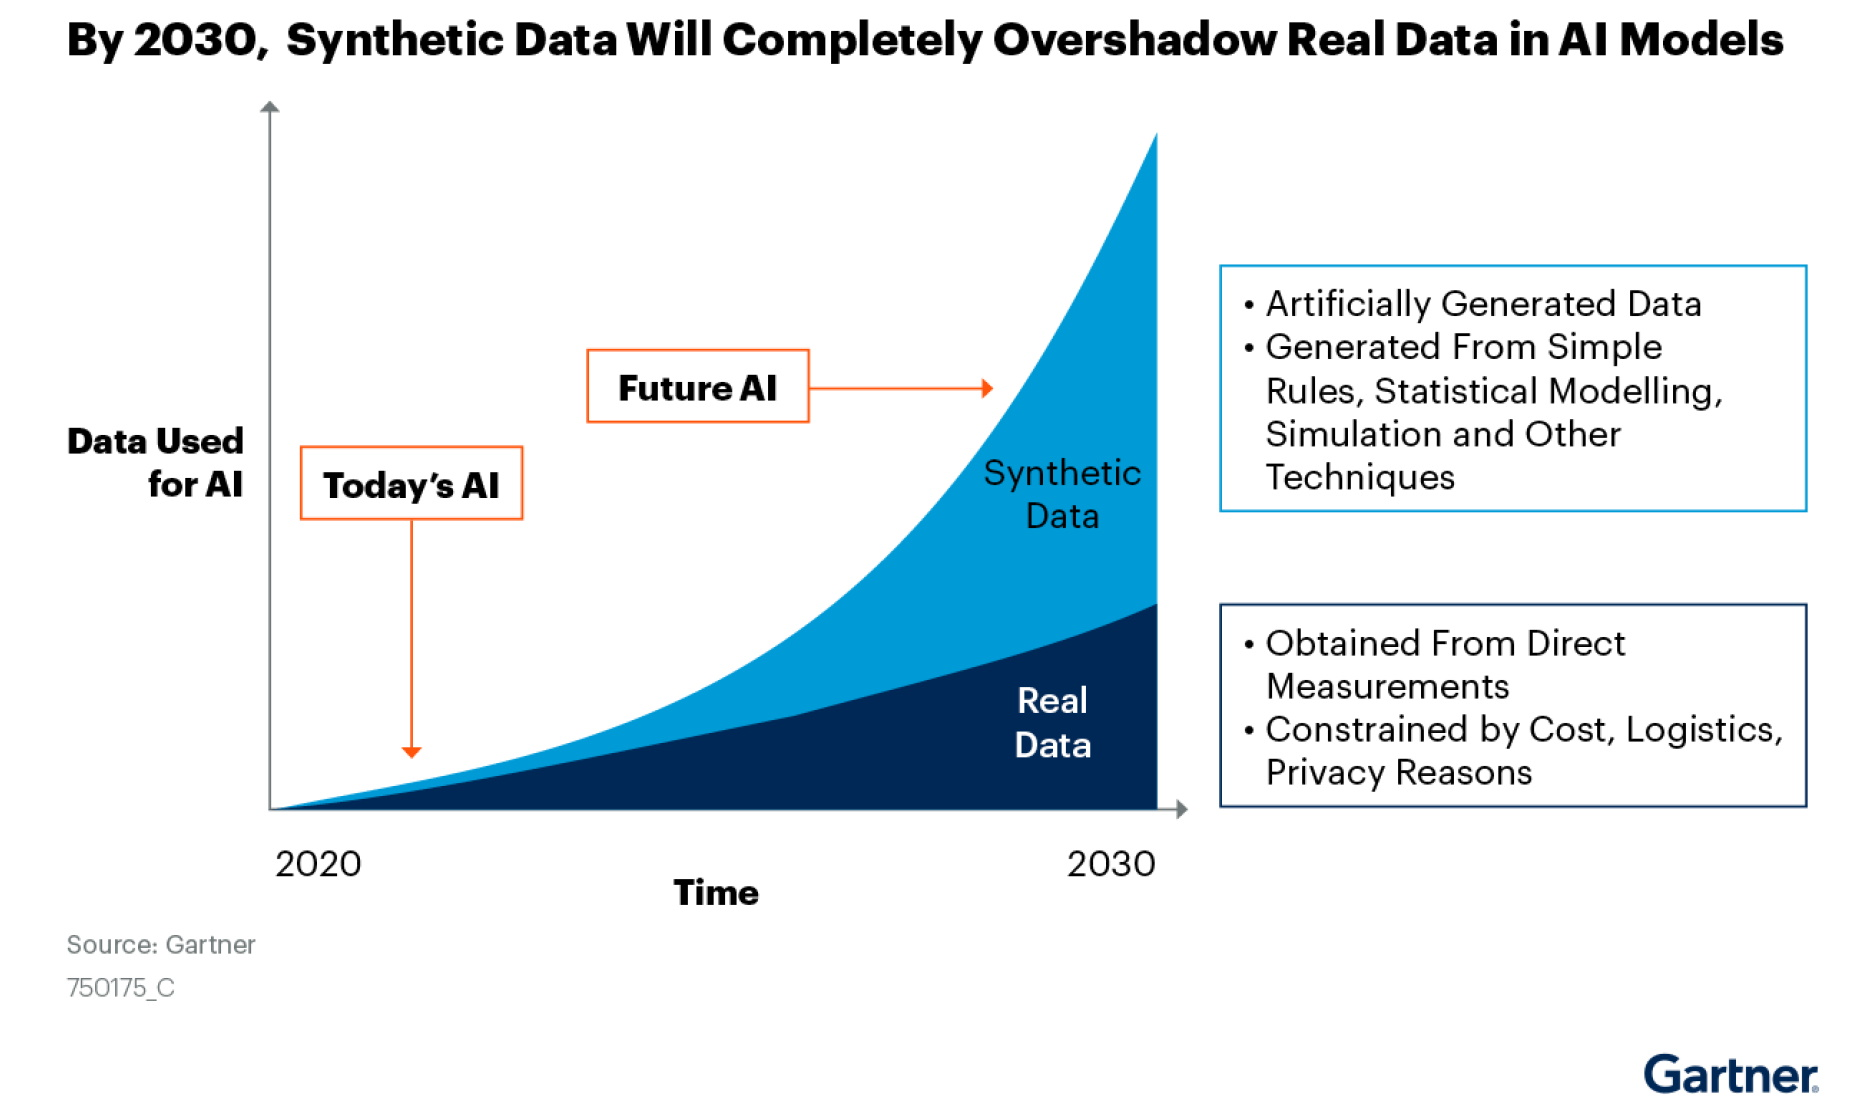
\includegraphics[width=0.75\textwidth]{images/synthetic-gartner.jpg}
    \caption{Synthetic data will become the main form of data used in AI \cite{gartner_inc2021synthetic}.
    }
    \label{fig:synthetic-data}
\end{figure}
    
Synthetic data is generated through simulations, algorithms, or computers, making the results independent of the experimenter. 
% A motivation for synthetic data is the 
A big misconception is that synthetic data can create a skewed image of scientific reality. This concern does not take into account, however, that data synthesis may have the potential to make scientific efforts more efficient. Data synthesis makes the research process more objective by providing a common ground for comparison and allowing experiments to be repeated, such as benchmarks. Additionally, synthetic data can improve the efficiency of experiments because the creation of the data does not have to be done repeatedly. Finally, synthetic data can also prevent researchers from falling into the trap of data dredging, which is when the researcher tests multiple hypotheses using a single dataset. In a June 2021 report on synthetic data\cite{gartner_inc2021synthetic}, Gartner predicted by 2030 most of the data used in AI will be artificially generated by rules, statistical models, simulations, or other techniques. This goes in conjunction and is supported by the breath-taking improvements in Unreal Engine 5's rendering pipeline \cite{unreal5_2021} to develop hyper-realistic 3D worlds, and the innovative advancements shown by Adobe in the past months (2020-2021) through their 3D Substance product line. Adobe 3D Substance includes thousands of models, textures, lighting systems, and uses artificial intelligence to reduce the technical complexity in 3D design and modelling \cite{adobe2021creative3D}. Synthetic data generation is not only a cost-saving technique but it can also sometimes even be better than real-world data, since it includes rare but critical corner cases in the distribution quality of a dataset. 

\begin{figure}[!ht]
    \centering
    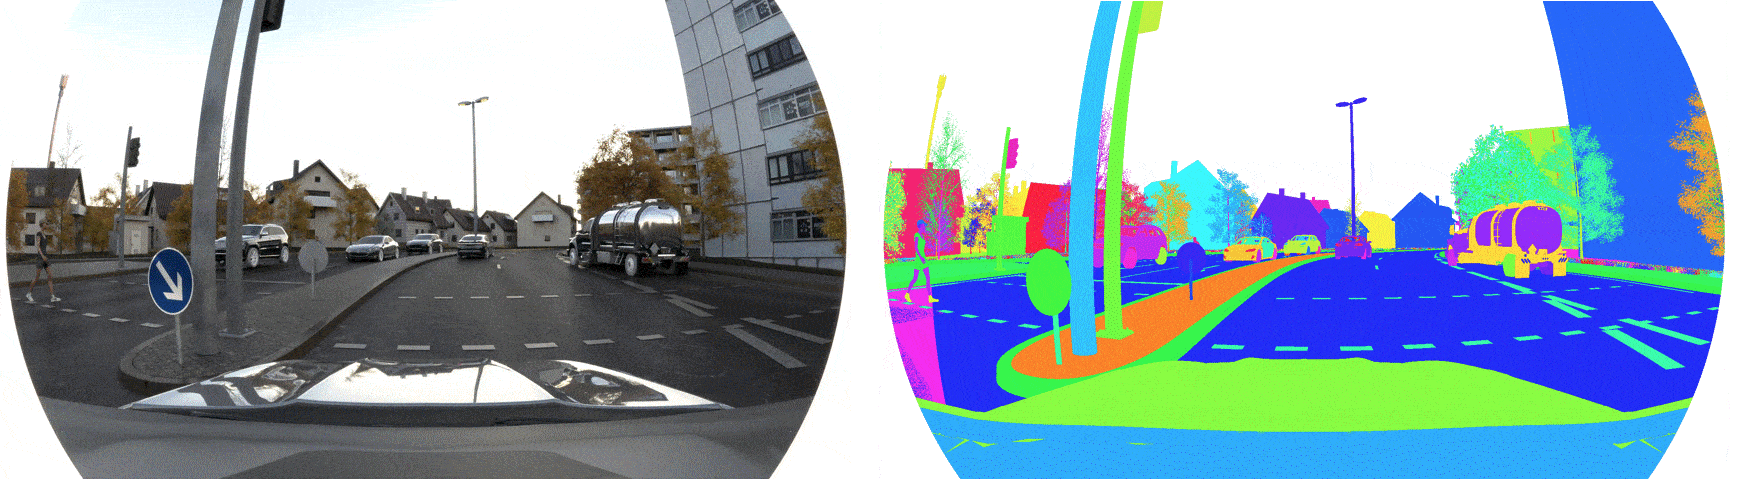
\includegraphics[width=0.95\textwidth]{images/synthetic-data.png}
    \caption{ Developers can alter and randomize objects, colors, lighting, materials and poses in realistic 3D environments to quickly generate synthetic data with perfect labels \cite{8_andrews_2021}.
    }
    \label{fig:synthetic-data}
\end{figure}
    
There are many techniques to generate synthetic data, such as variational autoencoder-decoders algorithms, GANs and simulations \cite{8_andrews_2021}. The factors mentioned in section \ref{chap2:gameengines} that make a good physics simulator such as domain randomization, texture randomization, noise simulation, etc., allow today's game engines to create sophisticated and realistic synthetic datasets, where algorithms and agents can learn more general patterns. Figure \ref{fig:synthetic-data} visualizes how developers and researchers are capable of manipulating 3D environments to generate realistic datasets with extensive domain randomization. It is therefore of special interest in this masters thesis to use the Unity 3D game engine to analyze exploration policies in simulated and realistic environments.
% We do so in three ways: (i) by first measuring the physical characteristics of the environment and the objects within it; (ii) by collecting data in a physical world; and (iii) by generating data in a digital world.


% The objective of this thesis is twofold: Firstly, I will present an implementation of a generative adversarial network that can be applied to create simulated physics based environments in Unity. Secondly, I will investigate how reinforcement learning can be applied to train such generative models in order to generate new data. For this, I will be focusing on the case of an agent that will be trained in the context of the LGP framework.

% The following sections will be organized as follows. In the first chapter, we will briefly discuss what is a generative model, GANs and their implementation in Unity. The second chapter

% https://blogs.nvidia.com/blog/2021/06/08/what-is-synthetic-data/
% https://searchcio.techtarget.com/definition/synthetic-data
% https://research.aimultiple.com/synthetic-data/



% new
\section{Reinforcement Learning}\label{chap2:reinforcement-learning}

Reinforcement learning is an umbrella term used to describe a class of algorithms for learning from experience. The basic idea is that a computer is given experiences in the real world (in a computer game, for example), and then has to learn how to act in that environment. The computer learns over time to increase its performance through trial and error and by watching what it does and making changes to its behavior policy. The performance is measured by the maximization of a reward function. Reinforcement learning is at the core of many of the most successful modern applications of artificial intelligence, such as AlphaGo, a computer that can play the board game Go better than any human being.

\begin{figure}[!ht]
    \centering
    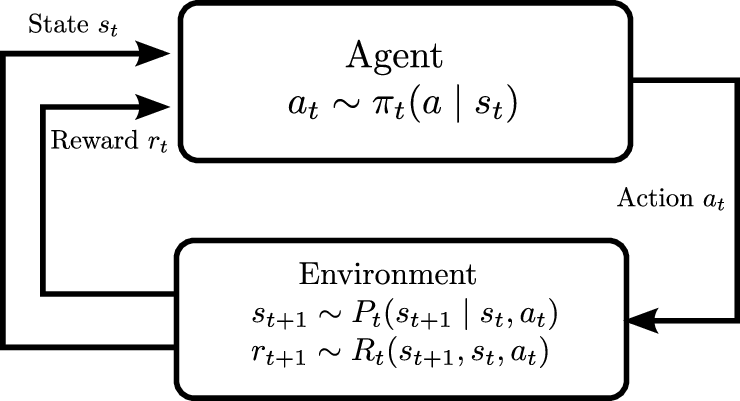
\includegraphics[width=0.50\textwidth]{images/agent-environment.png}
    \caption{Agent-environment relationship in an MDP according to \textcite{sutton1998introduction}: at each time step $t$, the agent observes the environment's current state $s_t$ and a reward signal $r_t$. The agent then selects an action $a_t$ given $s_t$ and following policy $\pi_t$. This action changes the environment state in the next time step to $s_{t+1}$ and yields reward $r_{t+1}$.
    }
    \label{fig:agent-environment}
\end{figure}


Despite the massive amount of recent research into the topic, reinforcement learning is still an extremely challenging field. This is due to the amount of information required to solve complex real world problems using reinforcement learning. For example, in the situation where one must create a simulation of a robot, one must take into account the factors and physics involved in the real world. 
% In fact, a recent paper on reinforcement learning concludes that, “The most common method for reinforcement learning involves learning the best policy in a simulated environment (or a set of them) through a brute force approach.”. 
% In fact, a recent paper on reinforcement learning concludes that, “The most common method for reinforcement learning involves learning the best policy in a simulated environment (or a set of them) through a brute force approach.”. 


Reinforcement learning is different from supervised learning in that the computer is given no labelled training data in the reinforcement learning case. Instead, it learns by trial and error and by watching its own actions. The idea is that, by observing what it does and seeing what results it gets, the computer will automatically learn what actions it should take to get better results in the future \cite{sutton2018reinforcement}.

% The subsections below describe 
Common concepts involved in a reinforcement learning problem are described below.

% Reinforcement learning is also referred to as a “model-free” learning algorithm. This is because the model that is learned, unlike in most other cases of machine learning, is not explicitly known beforehand


\textbf{Agent.}
The agent is the entity that actually does the learning. This is the actor that makes the decision for which action to take next based on the state observed from the environment \cite{sutton2018reinforcement}. For this action, the agent can receive a reward from the environment, from which the agent updates his value function or his policy. The agent then chooses a new action based on a new state and the interaction loop repeats. An complete interaction occurs at time step $t$, which is part of a sequence of time steps $t = 0, 1, ..., T$. 
The agent can be a single entity such as a robot or a group of entities that work together to solve the problem. The agent-environment interaction loop can be visualized in Figure \ref{fig:agent-environment}. 




\textbf{Action.}
The action refers to the action that is going to be taken. This could be one of the moves in a chess game, or it could be a move in a board game such as Go \cite{sutton2018reinforcement}.

\textbf{Learning from Experience.} The term “experience” as used in the context of reinforcement learning does not refer to a specific object or event. Rather, it refers to a sequence of events that have happened to the agent. However, the experiences that are fed into the reinforcement learning algorithm are derived directly from the environment \cite{sutton2018reinforcement}.

\textbf{Environment.}
The environment is the world in which the agent learns and collects observations of the state it finds itself in. It is also the world in which the agent must decide which actions to take. Accordingly, the environment provides rewards to the agent for each of these actions. Similarly, when the agent is, for example, damaged, the reward function decrements the reward that the agent receives for that action. The environment also provides the agent with feedback when it takes an action. It provides the agent with new visual observations, positions, velocity, health of enemy targets, etc. These observations are all factors that contribute to the agent’s perception of the environment. Environments, in general, can vary and be either a game of chess or a real-world application where one robot is being controlled by a human operator \cite{sutton2018reinforcement}.

A reinforcement learning environment can also be formally referred to as a Markov Decision Process (MDP) in other contexts, where each state is a possible outcome of the environment and each action is a possible change to the environment. 
An MDP is a formalism that can describe any decision-making process that can be described by a transition matrix. 
Moreover, for a reinforcement learning algorithm used in RL, an MDP may be thought of as a discrete-time Markov chain, where time is broken into discrete slots of a specified duration, and state is broken into discrete states.
This formalism allows a generalised analysis of the behaviour of an agent in terms of the utility or benefit of the agent in any state and any action taken in any state. It is described by a 5-tuple $(S,A,R,P,\mu)$, where:
\begin{itemize}
    \item $S$ is a set of states the environment can be in,
    \item $A$ is set of actions the agent can select,
    \item $R(s,a,s')$ is the reward function that maps state-action-next-state tuples to real valued rewards,
    \item $P(s'|s,a)$ is the probability of transitioning to state $s'$ given previous state $s$ and the agent choosing action $a$ while in $s$,
    \item $\mu(s)$ is the probability of starting in state $s$.
\end{itemize}
If an environment is fully observable, the agent has full knowledge of the state it is in. In a partially observable environment, the appropriate formalism is a Partially Observable Markov Decision Process (POMDP), where the agent must rely on its internal knowledge of its surroundings to make decisions. This is a generalization of the MDP to cases where the environment is partially observable, and it includes a set of observations $O$ and a conditional probability distribution, $P(o|s)$, for what observation is seen in which state \cite{sutton2018reinforcement}.


% There are two ways to make a policy in reinforcement learning. One way is to design a deterministic policy and then search through a set of possible actions (the policy). The other way is to search for an optimal policy, which is the solution to a dynamic programming equation. In both cases, there are two components that must be learned: the reward function and the value function. The reward function specifies the value of each action (change in state). The value

% The following figure illustrates the relationship between the environment and the agent, including the actions and observations that make up the state.

\textbf{Reward Signal and Return.}
A reward signal describes how well the agent did in a given situation. A reward signal can be thought of as a kind of scoreboard. It will assign a numerical score to each of the actions available to the agent in a given state. These scores are then combined to calculate a global reward which is to be maximized \cite{sutton2018reinforcement}.
In other words, the reward signal $R_t$ is the reward the agent obtains at time step $t$. The cumulative reward $G_t$ from this signal is the agent's objective. A simple return is defined as:
\begin{align*}
    G_t = R_{t+1} + R_{t+2} + ... + R_{t+T} = \sum_{k=0}^{T-t-1} R_{t+1+k}
\end{align*}
where T is the final time step. A return can also include a discount rate $\gamma$ that discourages future rewards:
\begin{align*}
    G_{t,discounted} = \sum_{k=0}^{T-t-1} \gamma^k * R_{t+1+k}.
\end{align*}
A discount rate is used, for example, if the MDP is a continuous problem that never ends or to include uncertainty of future predictions \cite{sutton2018reinforcement}.

\textbf{Value Function.}
Whereas the reward signal assigns a reward to the actions that are available to the agent at a given state, the value function specifies what is good in the long run. The value function calculates a value for a state, as the expected cumulative reward from the rewards in the future states, starting from that state. \cite{sutton2018reinforcement}
In other words, the state-value function, $V_{\tau}(s)$ is the expected future reward starting from state $s$ and following policy $\pi$. It can be written as

\begin{align*}
   V_{\pi}(s)=\mathbb{E}_{\pi}\left\{r_{t} \mid s_{t}=s\right\}=\mathbb{E}_{\pi}\left\{\left(\sum_{k=0}^{T-t-1} \gamma^{k} r_{t+1+k}\right) \mid s_{t}=s\right\}
\end{align*}
 
where $\gamma$ is the discount rate, $s_t$ is the state at time step $t$, $r_t$ is the reward at time step $t$, and $\mathbb{E}$ is the expected value \cite{eriksson2021deep}. 

Figure \ref{fig:gridworld} shows a grid-world environment where the agent must move from one cell to another to reach the goal. Given that there is a pit in which the agent can fall in. If the agent falls it is penalized through a negative reward. Hence, the state-value function for the cells around the pit is lower to represent that these are unwanted states.

\begin{figure}[!ht]
    \centering
    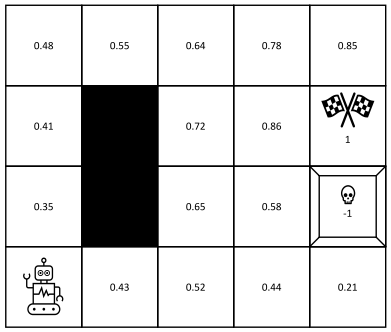
\includegraphics[width=0.55\textwidth]{images/gridworld.png}
    \caption{A grid-world environment \cite{eriksson2021deep}. Each cell represents a state, and it is associated with a corresponding value, which is the value of the state-value function $V(s)$. The agent gets a reward when it reaches the goal with two flags, and given a penalty when it falls down the pit with a skull.
    }
    \label{fig:gridworld}
\end{figure}



\textbf{Policy.}
The policy $\pi$ is the rule by which the agent decides which actions to take. In other words, a policy is a mapping from states to actions, and it defines how the agent will behave at any given state \cite{sutton2018reinforcement}.
The policy, just like the reward function, is learned based on what the agent experiences, i.e., what states provide higher reward than others. A policy can be designed as a look-up table or through function approximation. When the policy is stochastic $\pi(a|s)$ denotes the probability to take action a given state s, and the optimal policy $\pi*$ is the policy that always prefers the action corresponding to the highest expected reward \cite{sutton2018reinforcement}. 

% To make a decision, the agent looks at the environment and then selects an action from a set of actions. If there are multiple actions to choose from, then the agent randomly selects one of them.

\textbf{Episode.}
An episode\textemdash also called a \textit{trajectory} or \textit{rollout}\textemdash is a single event (i.e., the sequence of steps of an agent) which is composed of several time steps. An episode is defined by a sequence of states and a set of actions in an MDP \cite{sutton2018reinforcement}. For example, a video game will have many states (positions of objects, etc.), and many actions (movements of the character). 
% In Figure X an episode is comprised of the states the agent traversed, to reach a terminal state, which is when the episode ends. 
% These interactions agent-environment . In this sense, an episode is really a game.
% An episode ends when the agent reaches a terminal state.
At the end of an episode, the environment is reset and a new episode begins with a fresh set of observations and actions.

\textbf{Exploration and Explotation.}
Reinforcement learning problems try to balance exploration of new states and explotation by following the actions to states that provide the best rewards. Finding an optimal policy requires the agent to explore new unknown states which could allow the discovery of a better state-value than the one currently known. 
%  It cannot just sit in one spot and follow a pre-determined action sequence. It has to explore the environment and get to know it so that it can then use that knowledge to make good choices in future situations.
An example of a policy that prefers exploration is the $\epsilon$-greedy policy. This policy assigns $\epsilon$ chance to choose a random action and $1-\epsilon$ to choose an action based on the known policy \cite{sutton2018reinforcement}.  


\subsection{Q-learning} \label{chap2:q-learning}
Q-learning one of the most well known reinforcement learning algorithms. It is a model-free learning algorithm and therefore it does not require any assumptions to be made about the environment or about the reward function.
At the start of each episode, the agent picks an action (also called a “policy”) from some policy distribution. The agent then receives a reward which is calculated based on the policy that was chosen. The agent then uses the reward to update the policy distribution, which is often called the Q-function. The Q-function is an action-value function $Q_\pi(s,a)$, which, in addition to the state-value function (reference), it also considers the action space \cite{sutton2018reinforcement}. It can be written as:

\begin{align*}
    Q_{\pi}(s, a)=\mathbb{E}_{\pi}\left\{r_{t} \mid s_{t}=s, a_{t}=a\right\}=\mathbb{E}_{\pi}\left\{\left(\sum_{k=0}^{T-t-1} \gamma^{k} r_{t+1+k}\right) \mid s_{t}=s, a_{t}=a\right\}
\end{align*}

% Q-learning has proven to be a very successful and flexible algorithm, but it requires quite a bit of information to be provided in order to run efficiently.
Q-learning learns an optimal $\epsilon$-greedy policy. The agent has an $\epsilon$ chance of choosing a random action and $1-\epsilon$ of choosing an action based on the optimal policy. The optimal action is the one that maximizes the action-value function $\max _{a} Q_{\pi}(s, a)$ . 
% It algorithm starts
Q-learning works by starting from some arbitrary $Q_\pi(s,a)$, 
% state and action policy
and iteratively updates itself by taking into account the immediate rewards it receives. This is performed by taking an action and then updating its $Q_\pi(s,a)$ 
% policy distribution 
in the following manner:

\begin{align*}
   Q_{\pi}\left(S_{t}, A_{t}\right) \leftarrow Q_{\pi}\left(S_{t}, A_{t}\right)+\alpha\left[R_{t+1}+\gamma \max _{a} Q_{\pi}\left(S_{t+1}, a\right)-Q_{\pi}\left(S_{t}, A_{t}\right)\right]
\end{align*}

% $$\pi_{t+1}(s)=\frac{\pi_t(s)\cdot Q_\pi(s,a^*_t)}{\sum_{s'} \pi_t(s')\cdot Q_\pi(s',a^*_t)}$$

where $\lambda$ is the learning rate, $Q_\pi$ is the action-value function, and $\pi_t$ is the agent’s policy at step $t$. In the case of Q-learning, this is the optimal policy $\pi^*$. The learning rate determines how strongly the old values of $Q_\pi$ should be modified by the incoming update. This process is done until the episode ends. The environment then resets and the learning continues from a starting position \cite{sutton2018reinforcement}. The Q-learning algorithm can be seen in Algorithm \ref{alg:q-learning} below:

% \SetKwRepeat{Do}{do}{while}%


{\centering
\begin{minipage}{.8\linewidth}
    \begin{algorithm}[H]
      initialize $Q_\pi(s,a)$  with random values\;
      
      \For{each episode}{
        reset environment\;
    
          \While{\textbf{not} done}{
            choose action A based on state S using policy \pi\;
            
            perform action A and observe R,S'\;
            
            $Q_{\pi}(S, A) \leftarrow Q_{\pi}(S, A)+\alpha\left[R+\gamma \max _{a} Q_{\pi}\left(S^{\prime}, a\right)-Q_{\pi}(S, A)\right]$
            
            $S \leftarrow S^{\prime}$
            
            \If{episode end}{
                done\;
            }
          }
      }
      \caption{Q-learning}\label{alg:q-learning}
    \end{algorithm}
\end{minipage}
\par
}


After $n$ episodes, Q-learning should be able to learn a policy that allows the agent to solve the task successfully. There are several variants of Q-learning that differ from the method described above. A popular variant of Q-learning is SARSA (“Synchronous”, “Asynchronous”, “Reinforce”), which can be used for learning both discrete (e.g. chess, Go) and continuous (e.g. Atari games, robotics) problems \cite{sutton2018reinforcement}. Additionally, it is one of the algorithms available in the open source deep reinforcement learning OpenAI Gym \cite{openaigym}.

% https://deepsense.ai/what-is-reinforcement-learning-the-complete-guide/
% https://www.geeksforgeeks.org/what-is-reinforcement-learning/
% https://www.kdnuggets.com/2018/03/5-things-reinforcement-learning.html

% new

\subsection{Function Approximation}\label{chap2:function-approx}
Tables are a feasible solution for small state space searches for state-value and action-value functions. However, when the state space is large, such as in robotics applications, tables become impractical. 
Function approximation methods such as Gaussian processes, neural networks, and deep neural networks, make it easier to approximate large state-value and action-value functions \cite{sutton2018reinforcement}.
% were developed to work around this problem. 

% \textbf{Gaussian Processes.} 
% When a function  is continuous it can be approximated by a linear combination of Gaussian random variables. Let  be a Gaussian distribution with covariance function  such that  is a valid  for all  with probability. A Gaussian Process is a collection of  with  and  for any valid, and thus,  is a valid function approximator. The Gaussian process is useful for problems that are not known beforehand. The predictive distribution is given by

% where  is a multivariate Gaussian with mean  and covariance matrix  and  is a collection of  such that.

\subsubsection{Neural Networks.}
Neural networks are particularly good for modeling nonlinear relationships as they are essentially universal approximators.
They use a large number of interconnected neurons (perceptrons) to approximate the function $y = f*(x, \theta)$, which defines a mapping from input $x$ to output $y$, by learning the parameters $\theta$ \cite{eriksson2021deep}.

\begin{figure}[!ht]
    \centering
    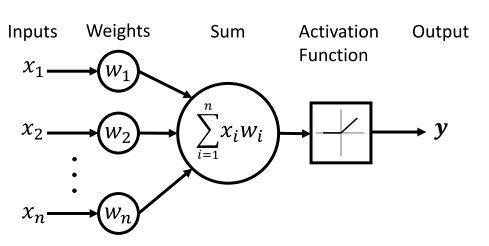
\includegraphics[width=0.5\textwidth]{images/neuron.png}
    \caption{Neuron. A single neuron consists of an input (or data) connection and an output (or hidden) connection. The input $x$ is multiplied by the training weights $\theta$ and summed. An activation function is then applied to the sum to obtain a nonlinear function $h(x,\theta)$ of the inputs.}
    \label{fig:neuron}
\end{figure}


    
A neuron consists of an input (or data) connection, and an output (or hidden) connection, as visualized in the model in Figure \ref{fig:neuron}. Inputs $x$ are multiplied by a set of training weights $\theta$ and summed. An activation function $h$ is then applied to the sum. The output $h(x,\theta)$ of a neuron is a nonlinear function of the input, and as a result a large number of neurons is needed to approximate a complex function. The weights are then trained by backpropagation in order to minimize the cost of the function approximation (i.e. the training set error). A common activation function, ReLU is defined as follows:
\begin{align*}
    h(x,\theta) =
    \begin{cases}
        0 & \text{if } z < 0,\\
        z & \text{if } z \ge 0,\\
    \end{cases}
\end{align*}
% then a neuron receives a set of inputs $v_i^j$ and returns an output $z_i^j$. The outputs are then combined with other outputs to form a neuron’s final output $o$.
% in continuous state space problems since they are relatively easy to train by back-propagation using a loss function.
where z is the summed output of the neuron. By tuning the weights of a neural network, non-linear functions can be approximated. Accordingly, a neural network could be leveraged to approximate the value function or policy of an agent by feeding state $s$ as input to the network \cite{eriksson2021deep}. 
% The weights of a neural network can be tuned through gradient descent.
A common and efficient method to tune the weights of a neural network is batch gradient descent. Gradient descent can be defined as
\begin{align*}
    \theta_{i, j} \leftarrow \theta_{i, j}-\alpha \frac{\partial L}{\partial \theta_{i, j}}
\end{align*}
where $\alpha$ is the learning rate, $\theta_{i,j}$ are the neural network's weights and $L$ is the loss function.
A loss function is a measure of how well the neural network approximates the desired function. Common loss functions for value functions include squared error and mean squared error, where common loss functions for policy functions is cross-entropy. In the squared error $L=(y-\hat{y})^{2}$, $\hat{y}$ is the predicted output from the network and $y$ is the true value (ground truth).  For more information on backpropagation and gradient descent, see \cite{sutton2018reinforcement}. 

% Figure X: 
% Neuron with data input $x$ and hidden output $h$.

Neural networks have been shown to be a very powerful approach to nonlinear function approximation. For example, they are able to approximate the square root, logarithm, exponential, etc. However, this is not the case for complex functions, such as $f(x, \theta) = 1/1 + x \cdot \sin(\theta)$. While neural networks are an important tool in reinforcement learning, they are only good for low-dimensional functions and cannot be directly applied to high-dimensional or discrete state spaces. This has led to the emergence of methods using deep neural networks \cite{sutton2018reinforcement}.


% \textbf{Deep Neural Networks.}A deep neural network can be viewed as two neural networks or more, which are called hidden layers. The input data is the input layer and the predictions layer is the output layer. 
% The structure of a deep neural network is given by where and how layers interconnected. 
% Deep neural networks, as mentioned before, are trained by back-propagation

% Reinforcement learning is most successful when the value functions are approximated as neural networks, which is the focus of this work.

% In this case, it can be shown that the value function must satisfy the Bellman equation:
% Two popular function approximation methods are neural networks and Q-learning.
% https://www.baeldung.com/cs/ml-policy-reinforcement-learning#:~:text=A%20policy%20is%2C%20therefore%2C%20a,agent%27s%20state%20and%20the%20environment.
% https://towardsdatascience.com/policy-based-reinforcement-learning-the-easy-way-8de9a3356083

\subsubsection{Deep Neural Networks}
%  Accordingly, as the layers are stacked on top of each other, the number of parameters and amount of information needed to define the parameters increases. 

\begin{figure}[!ht]
    \centering
    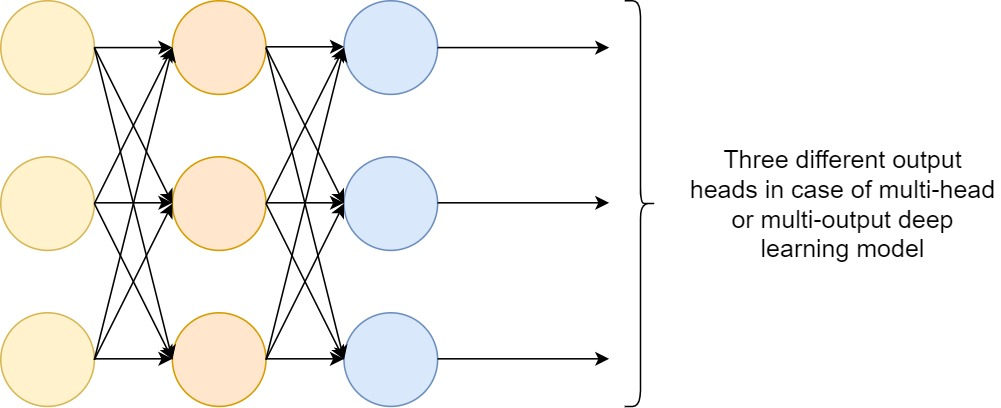
\includegraphics[width=0.7\textwidth]{images/multi_head_nn_exmp.jpg}
    \caption{Deep Neural Network with an input layer, a hidden layer and an multiple output heads. In actor-critic reinforcement learning problems and shared parameter networks, one head can be used as the prediction from the critic and another head as the prediction from the actor \cite{MultiHea51, sutton2018reinforcement}.
    }
    \label{fig:deep-nnetwork}
\end{figure}


Deep neural networks are a type of neural network which have been shown to work well for a variety of real world problems. In general, deep neural networks are a type of neural network that uses multiple layers of interconnected neurons, as shown in Figure \ref{fig:deep-nnetwork}. 
In situations when the input is an image, data manipulation strategies can be used, such as vectorization of the image so that it is compatible with the input a simple neural network expects. However, the loss of spatial information during the vectorization of the data (also called flattening) can be a problem if part of the solution requires to understand the relationship between the elements in a scene. Convolutional neural networks have therefore been shown to be a very effective solution to this problem since they are capable of processing images while keeping their matrix structure. These networks use a kernel of weights to "convolute" the image, which is also called "filter". A filter is applied over the entire input to output a new set of values. This process is repeated over all the different parts of the input and can be then fed to other types of network structures, such as fully connected layers \cite{eriksson2021deep}.
As of today, convolutional neural networks have proven to work well in many different domains, such as image classification, object detection, and semantic segmentation.


\subsection{Proximal Policy Optimization}\label{chap2:ppo}
Proximal Policy Optimization (PPO), designed by OpenAI, is a reinforcement learning algorithm that is known for performing better than one of the most popular reinforcement learning algorithms: DQN (also known as the Deep Q Network algorithm; which has roots in the theory presented in Section \ref{chap2:q-learning}).
PPO overcomes a lot of challenges that other methods struggle with such as sample efficiency, overall performance, and ease of implementation and tuning capabilities \cite{schulman2017proximal}. %16, 17 
Moreover, while algorithms like DQN learn from offline memory, PPO can do online learning without using a replay buffer for past experiences. In other words, it allows the agent to learn directly from the environment and discard the batch of experiences after a gradient update. 
Finally, PPO belongs to methods that leverage the state value function to update the policy. Actor-critic methods, as an extension of Q-learning, approximate the value function (critic) to assist in the policy (actor) updates.

The following subsections further introduce the fundamental concepts behind PPO, such as policy gradient and clipping, and the algorithm itself.


% Reinforcement Learning Algorithms

% Actor-Critic

% The actor-critic algorithm is an offshoot of PPO and is a more efficient variant of PPO. The algorithm uses both a

\subsubsection{Policy Gradient}
Policy Gradient methods estimate the optimal parametrized action policy $\pi(a \mid s, \theta)$ (i.e. which action is taken in each state) and are typically used in large state spaces. These methods learn the policy's parameter vector $\theta$ by learning the weights of a neural network. 
The parametrized policy $\pi(a \mid s, \theta)$ describes a distribution which gives a probability of choosing action $a$ given state $s$ and parameters $\theta$ at timestep $t$ as
\begin{align*}
    \pi(a \mid s, \theta)=\operatorname{Pr}\left\{A_{t}=a \mid S_{t}=s, \theta_{t}=\theta\right\}.
\end{align*}
These methods aim to maximize the expected return $J(\theta)$, known also as the objective function or loss, by following the parametrized policy \cite{sutton2018reinforcement}. Gradient descent (or ascent) is then used to update the weights of the network as
\begin{align*}
   \theta_{t+1}=\theta_{t}+\alpha \widehat{\nabla J\left(\theta_{t}\right)}
\end{align*}
where $\widehat{\nabla J\left(\theta_{t}\right)}$ is an estimate of the gradient of the objective function (expected return) \cite{3}. A standard gradient estimator for these methods is
\begin{align*}
    \widehat{\nabla J\left(\theta_{t}\right)}=\hat{E}_{t}\left[\nabla_{\theta} \log \pi_{\theta}\left(a_{t} \mid s_{t}\right) \hat{A}_{t}\right]
\end{align*}
where $\pi_{\theta}$ is the parametrized stochastic policy, $\hat{E}_{t}$ is the expectation across a batch of experiences and $\hat{A}_{t}$ is an estimator of the advantage function at timestep t \cite{sutton2018reinforcement}. 
The respective objective function for the policy gradient estimator is therefore
\begin{align*}
  L^{\mathrm{PG}}(\theta)=\widehat{J(\theta)}=\hat{E}_{t}\left[\log \pi_{\theta}\left(a_{t} \mid s_{t}\right) \hat{A}_{t}\right].
\end{align*}
Optimizing on $L^{P G}$ is, however, not justified, given that it leads to destructively large policy updates \cite{schulman2017proximal}.

\subsubsection{Clipping}
PPO builds upon the concepts mentioned above and simplifies the concepts introduced by TRPO by proposing a clipped "surrogate" objective and retaining parallel performance. 

\begin{figure}[!ht]
    \centering
    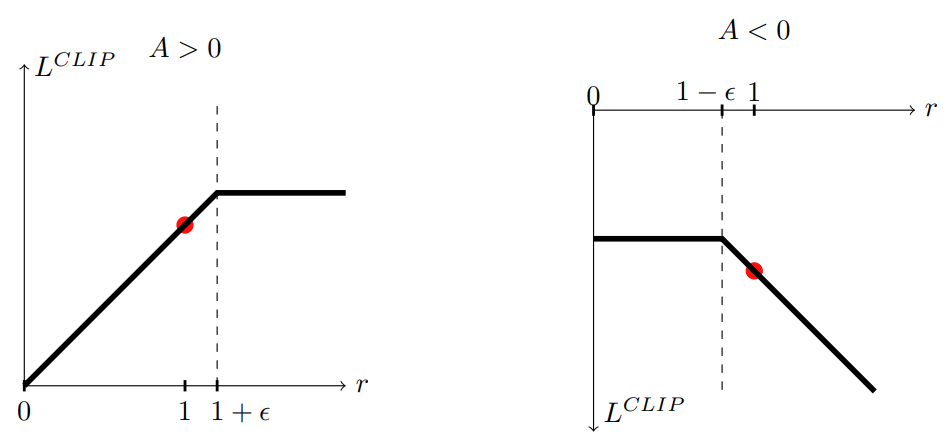
\includegraphics[width=0.7\textwidth]{images/LCLIP_PPO.png}
    \caption{Plots showing one term (i.e., a single timestep) of the surrogate function L CLIP as a function of the probability ratio r, for positive advantages (left) and negative advantages (right). The red circle on each plot shows the starting point for the optimization, i.e., r = 1. Note that L CLIP sums many of these terms.
    \cite{schulman2017proximal}.
    }
    \label{fig:LCLIP}
\end{figure}

First, the probability ratio between the policy with the current parameters and the policy with the old parameters is defined as
\begin{align*}
    r(\theta)=\frac{\pi_{\theta}(a \mid s)}{\pi_{\theta_{\text {old }}}(a \mid s)}.
\end{align*}
Then, the objective function of TRPO (on policy) is:
\begin{align*}
  L^{\mathrm{TRPO}}(\theta)=\mathbb{E}\left[r(\theta) \hat{A}_{\theta_{\text {old }}}(s, a)\right].
\end{align*}
However, given that the ratio between the policies can grow to be very large, PPO constraints the ratio $r(\theta)$ to stay in a small interval around $1$ through the introduction of an additional hyperparameter $\epsilon$ \cite{schulman2017proximal}. The value function loss then becomes
\begin{align*}
    L^{\mathrm{CLIP}}(\theta)=\mathbb{E}\left[\min \left(r(\theta) \hat{A}_{\theta_{\mathrm{old}}}(s, a), \operatorname{clip}(r(\theta), 1-\epsilon, 1+\epsilon) \hat{A}_{\theta_{\mathrm{old}}}(s, a)\right)\right]
\end{align*}
where the function $\operatorname{clip}(r(\theta), 1-\epsilon, 1+\epsilon)$ constraints the ratio to a maximum and a minimum. Subsequently, the objective function of PPO takes a pessimistic lower bound to the loss by keeping the minimmum of the unclipped $r(\theta) \hat{A}_{\theta_{\text {old }}}(s, a)$ and the clipped ratio times the advantage estimator \cite{schulman2017proximal}. The advantage estimator is defined by
\begin{align*}
  \hat{A}_{t}=\delta_{t}+(\gamma \lambda) \delta_{t+1}+\ldots+(\gamma \lambda)^{T-t+1} \delta_{T-1}
\end{align*}
where
\begin{align*}
  \delta_{t}=r_{t}+\gamma V(s_{t+1})-V(s_{t})
\end{align*}
and $\lambda$ is a smoothing coefficient. 
  
% \subsubsection{Policy Iteration}
% Policy Iteration is a model-based algorithm for reinforcement learning. Unlike the model-free Q-learning algorithm, it assumes a model of the environment. The agent can then perform actions and the agent’s behavior can be calculated by performing an appropriate simulation of the environment. When it receives the environment’s observation, the agent can determine whether it believes the environment is in a certain state or not. The agent then performs actions and the environment responds. This process is repeated multiple times and the agent’s reward is calculated. The reward can then be used to update the environment model. The process of learning from experience can be summarized by the following algorithm.

\subsubsection{Algorithm}
% A common practice to reduce the variance of the gradient of the expected return estimates is to add a baseline function $b(st)$ inside the expectation. Typical choices are the average reward $\bar{R}$, or the state value function $V(s)$. For more information on baseline functions, refer to \cite{}.
Most techniques for calculating variance-reduced advantage-function estimators leverage a learned state-value function V(s) as baseline function and PPO is no different \cite{schulman2017proximal}. If using a neural network architecture that shares parameters between the two predictions heads for the policy and value functions, PPO proposes to add a value function error term to the policy surrogate and an entropy term to encourage sufficeint exploration. This new loss is defined as
\begin{align*}
    L_{t}^{C L I P+V F+S}(\theta)=\hat{\mathbb{E}}_{t}\left[L_{t}^{C L I P}(\theta)-c_{1} L_{t}^{V F}(\theta)+c_{2} S\left[\pi_{\theta}\right]\left(s_{t}\right)\right]
\end{align*}
where $c1$,$c2$ are coefficients, $S$ denotes the entropy bonus and $L_{t}^{V F}$ is the value function loss \cite{schulman2017proximal}. In other words, $L_{t}^{C L I P}(\theta)$ is the loss for the actor network and $L_{t}^{V F}$ is the loss for the critic network. The loss of the value function used in PPO is defined as
\begin{align*}
    L^{\mathrm{VF}}=\left(V_{\theta}\left(s_{t}\right)-V_{t}^{\text {target }}\right)^{2}
\end{align*}
where $V_{\theta}\left(s_{t}\right)$ is also known as the critic return and in some implementations is seen as $\delta_{t} + V_{\theta}\left(s_{t}\right)$. Similarly, the term $S_{\pi_{\theta}}\left(s_{t}\right)$ is an entropy bonus that promotes exploration \cite{schulman2017proximal}. Concretely, this is the Shannon entropy and is computed by
\begin{align*}
    S_{\pi_{\theta}}\left(s_{t}\right)=-\sum_{i=1}^{n} \pi_{\theta}\left(a_{i} \mid s_{t}\right) \log \left(\pi_{\theta}\left(a_{i} \mid s_{t}\right)\right.
\end{align*}
In summary, the main idea of PPO is to avoid large policy updates during training by clipping the ratio between the old and the current policy. It successfully combines function approximation with policy optimization while showing great performance \cite{schulman2017proximal}. Finally, the algorithm is described in Algorithm \ref{alg:ppo} below:

{\centering
\begin{minipage}{.8\linewidth}
    \begin{algorithm}[H]
        initialize $\theta$\;
      
        \For{iteration i=0,1,...}{
            \For{time step t=0,1,..., T}{
                sample time step with policy $\pi_{\theta, \text { old }}$\;
                calculate advantage $\hat{A}_{t}$\;
            }
            \For{epoch k=0,1,..., K}{
                optimize $L^{\mathrm{CLIP}+\mathrm{VF}+\mathrm{S}}$ with respect to $\theta$\;
                update $\theta$\;
            }
        }
      \caption{PPO}\label{alg:ppo}
    \end{algorithm}
\end{minipage}
\par
}



%  The environment includes a simulation of the voxels, such that voxel positions have a value (e.g. their distance to a goal voxel) which changes based on actions in the environment. Voxel positions also have an octree node in which they are embedded. This allows the voxels to have a 3D spatial location in the environment. The voxels are also assigned a classification (e.g. “rock”, “fertilizer”, “air”, etc.). The voxels also receive a reward which is related to the classification they represent

%  We formulate the reinforcement learning problem as one of minimizing a loss function defined on exploration and goal selection. Specifically, the exploration policy is a probability distribution that selects the voxel from the voxel pool to observe based on their classification. The goal is a set of octree nodes, which are a tree in which each node has an octree parent node and a set of child nodes that are octree children nodes of the parent node. For each goal node, there is an associated reward value.


% In the simplest scenario, the goal is always the goal node. We propose two different models of goal selection. The first model is a fully deterministic approach where a goal node is randomly selected from the goal set. The goal nodes are randomly ordered before being selected from the goal set, and the order of nodes can be randomized. The second model is a semi-deterministic approach where a goal node is selected based on a probability distribution from a goal distribution. The goal distribution is defined by a Gaussian kernel function which is used to select nodes from a set of nodes in a specific region of the environment.

% deterministic
% semi-deterministic



% method (old)
% based on actions in the environment. Voxel positions also have an octree node in which they are embedded. This allows the voxels to have a 3D spatial location in the environment. The voxels are also assigned a classification (e.g. “rock”, “fertilizer”, “air”, etc.). The voxels also receive a reward which is related to the classification they represent.

% we train the agent with a genetic algorithm [@mouret]



% method, solid
% Reinforcement learning is an umbrella term used to describe a class of algorithms for learning from experience. The basic idea is that a computer is given experiences in the real world (in a computer game, for example), and then has to learn how to act in that environment. The computer learns over time to increase its performance through trial and error and by watching what it does and making changes to its behavior policy. In our context, reinforcement learning means learning how to generate exploration policies given intrinsic rewards based on voxels and octree nodes in an unknown environment.

% The environment includes a simulation of the voxels, where every voxel has been generated through a voxel generating algorithm that traversed the original mesh of each object. Moreover, each voxel has a position and a pose (e.g. near the mesh of the object it belongs to) which remains set until the end of an episode. An episode can end when the agent hits a wall or all the voxels have been scanned. Once an episode ends, domain randomization allows to change the locations and poses of the objects of interest, to promote the generalized exploration of unknown environments.


% Our agent can therefore learn how to behave in the voxel-based environment, while also embedding the positions it traverses and the positions of the scanned voxels in the nodes of an octree. This motivates the agent to explore new nodes in the environment, both with and without voxels. The voxels are therefore not assigned any classification (e.g. "rock, "fertilizier", "bike", etc.). Instead, they are concrete 3D representations of the objects of interest to the agent, which serve as intrinsic rewards to the agent. Ideally, the voxels would provide a different reward related to the classification they represent, but the semantic to each object has been determined out of scope to focus rather in a general exploration of the environment.

% another wording
% The problem of reinforcement learning is therefore a multi-agent interaction problem. In our case, a single agent is in charge of the whole process and tries to maximize its cumulative reward over time. The agent interacts with the environment and learns from its experience by choosing actions that maximize its rewards. As it is more likely that it is more beneficial for the agent to explore than to stay within a known area, the environment rewards the agent for exploration. To promote generalization, we allow the agent to explore the environment in an incremental manner: the environment randomly changes the positions of the objects of interest in the simulation, and the agent is not

% In order to demonstrate AEIL, I will take the case of a computer simulation where the goal of the robot is to traverse a maze. While this is a trivial task in the real world, for the sake of the experiment, the maze is a simulation of the real world. The maze is divided into an x-axis and a y-axis, with all obstacles located at one of the endpoints. As with real life, the maze is generated randomly, and the computer learns as it moves forward. In this case, the computer starts from the top left corner of the maze, and the goal is to find a way

\chapter{Octree- \&
Voxel-driven Exploration}\label{chap:3:title}
% \chapter{Method}\label{chap:3:title}

\begin{figure}[!ht]
        \centering
        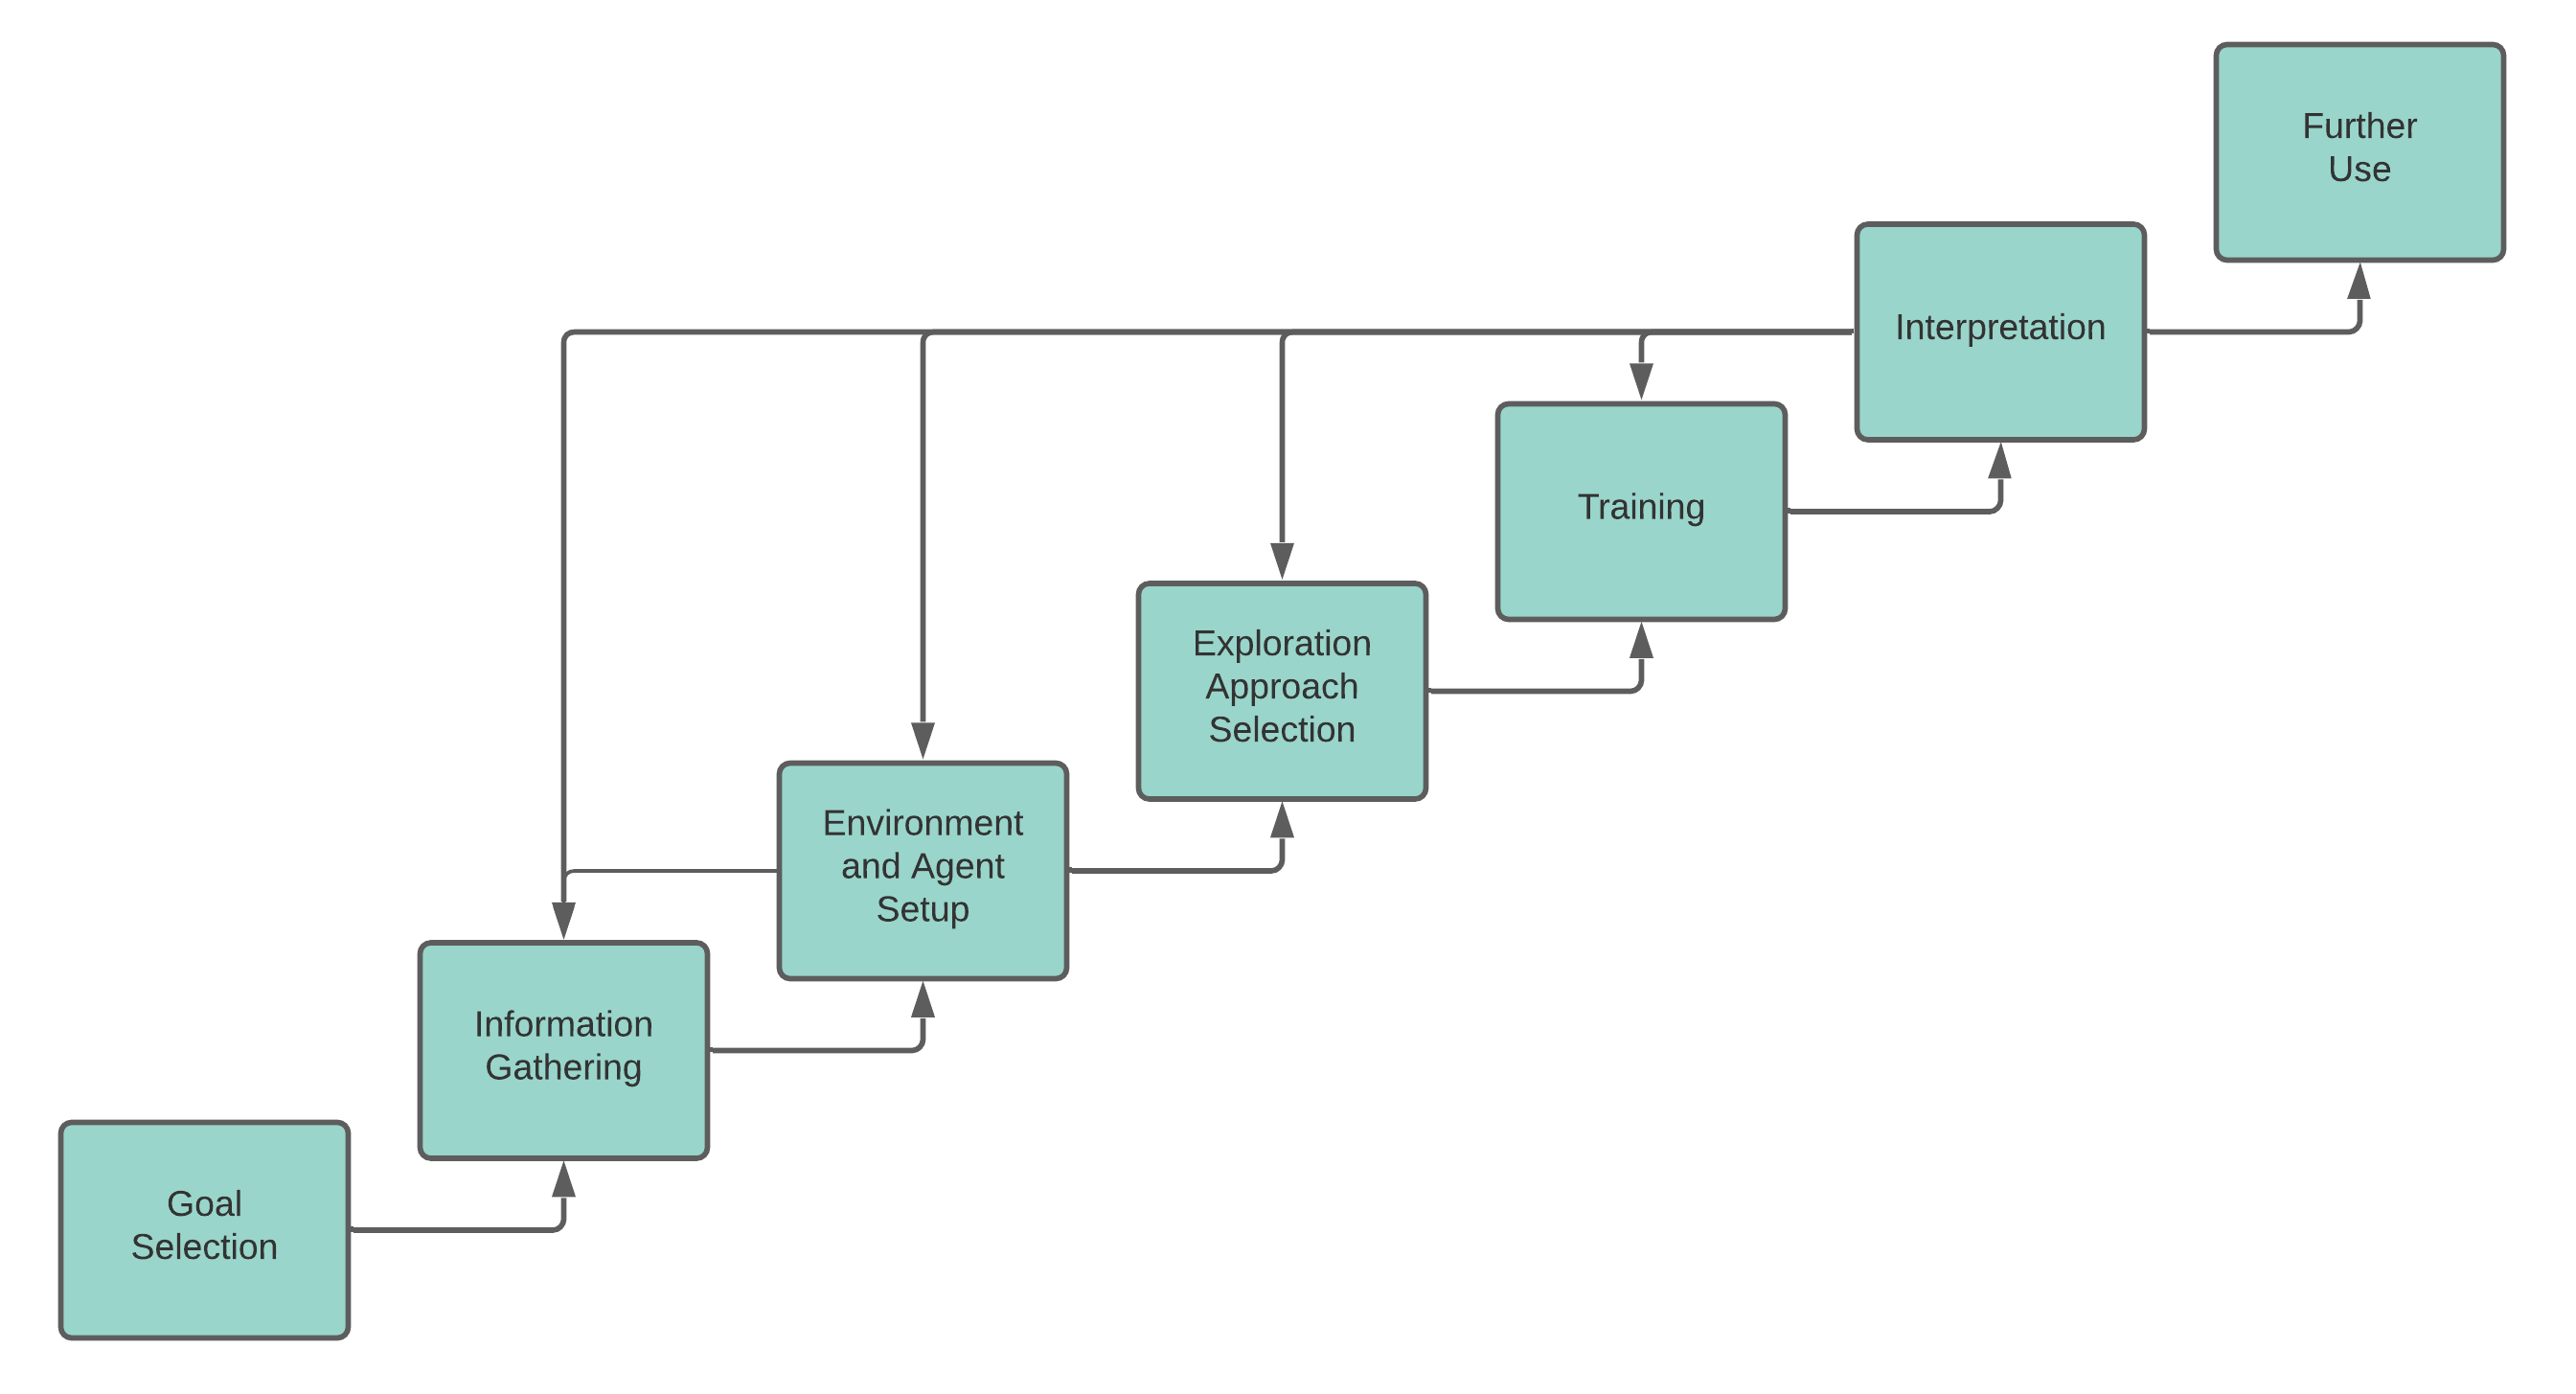
\includegraphics[width=1\textwidth]{images/adapted_development_process_exploration_v2.png}
        \caption{Adapted development process from "\citetitle{luckert2016using}", by \textcite{luckert2016using}. Describes the taken steps from data collection, through algorithm selection to architecture design.}
        \label{fig:development_design}
\end{figure}
In this chapter, the different steps taken to construct the environment and the reinforcement learning agent are addressed. 
This chapter adapts the structure proposed for machine learning algorithms proposed by \textcite{luckert2016using}.
The following questions are answered during this chapter:
\begin{itemize}
    % \item What kind of data is necessary?
    % \item What is the process for modeling 3D environments for exploration?
    % \item What are the 
    \item What are the current method's goals and limits?
    \item How was the reinforcement learning environment modeled and set up?
    % \item How was the agents perception defined?
    \item How is the agent-observable data constructed?
    % \item How are voxels generated from RGBD data?
    % \item What is Unity ML Agents for reinforcement learning?
    \item How was the agent's character defined (3D model, movement, etc.)?
    \item What reinforcement learning approach was chosen? 
    \item How is the proposed method composed? 
    % what method (of all the compared ones) provides the possibility to answer the research questioon and how is it composed? ....
    % \item What is the method's pipeline composed of?
    % \item What attributes apply to the learning agent?
    \item How can the proposed exploration method be further applied?
\end{itemize}


In order to answer these questions, the structure of this chapter is illustrated in Figure \ref{fig:development_design}.
The first step of the RL process is discussed in Section \ref{chap:3:goal}, which defines the exploration task and limits its scope. 
Then, the choice of a suitable 3D environment for exploration where the agent collects observations from (i.e., the data set) and the construction of the 3D environment is presented. 
% collected raw data as
Section \ref{chap:3:data} introduces the modeling process and setup of the 3D environment.
% /the 3D assets, components and variables that compose the environment.
% information available (voxels, octree data) and the choice of observations for the given task
Afterwards, it explains the approach to perception, presenting the process of voxelization, the creation of the octree map.
% , the grid sensor component and the concept of semantic entropy.
Then, it outlines the sensors used in the agent for visual input and the usage of semantic entropy to define uncertainty in an environment.
% 
% preprocessing of the data by identifying noise or erroneous inputs. 
% preesents the choiceof three proposed processing pipelines and the considered algorithms and techniques. T
The agent's character, including 3D models, movement algorithms and other components are presented in Section \ref{}.
Furthermore, the choice of agent observations, reward signal and environment-related behaviors are defined in Section \ref{chap:3:agent-choice-actions} and the description of the chosen reinforcement learning algorithm is covered in Section \ref{chap:3:specification-approach}. Subsequently, the interpretation of the exploration approaches to octress and voxels are described in Section \ref{chap:3:interpretation}. 
This section also tackles how the method's performance was measured and evaluated and which parameters were tuned.
% the algorithms were compared to each other
Finally, Section \ref{chap:3:further-use} presents the proposed evaluation framework for the assessment and comparison of the learned behaviors, introduces the applicability of our approach in multiple scenarios, presents the transferability of the learning environment to another environment platform and proposes the comparison of the performance of the PPO with the Soft Actor-Critic algorithm for the given setup.
% for the experiments to evaluate and compare learned behaviors.
% dacross for determining the 3D position of the salient object. 
% It also sets out the assumptions we took and the choices of technologies with respect to what was discussed in Section 2.
Inspired by the structure proposed by \textcite{luckert2016using} and given the iterative nature of the reinforcement learning process, this work was split into two main loops:
\begin{itemize}
    \item The first loop includes steps 2 and 3, and involves the groundwork for the learning algorithm: it involves the manual construction of the learning environment and the agent using Unity \cite{unity2021} for fabricating the 3D scenes and the ML-Agents SDK \cite{github-unity-mlagents-toolkit}. This resulted in a high dependency between the 3D modeling, the simulation of a real robot and the  abstractions provided by the learning platform, which demanded an iterative development process.
    
    \item The second loop includes steps 2-6, which allows the readjustment of 3D models, the learning environment, agent attributes, observations, reward signals, step size, voxel models, octree parameters, entropy definition, etc. This loop is critical for this thesis, since the main objective is the optimization of exploration strategies for unknown environments. For this purpose, the presented iterative process was used and multiple baselines were proposed to provide performance comparisons. Furthermore, the diverse algorithms performance can be inspected in real-time in Unity and therefore require readjustments in steps 2 and 3.

    % can be explained through the working loop illustrated in Figure \ref{development_design}. This loop allows the 
\end{itemize}

% domain model
%  
\section{Identification of Goals}\label{chap:3:goal}
The predetermined goal of this project work was to propose an exploration policy that reduces uncertainty in a 3D scene. As mentioned in Section \ref{chap:1:research-question}, this project work tackles the following research questions: 
\begin{itemize}
    %  Howcan an active vision exploration policy based on a ubiquitous source of information such as voxels, in currently accessible RGBD cameras, contribute to reducing the uncertainty about a scene?
     % \item How can these exploration policies be leveraged for a multitude of scenarios, including the milking robot problem? 
   
    % \item How can 3D data (meshes or point clouds), in voxel form, be exploited for extrinsic motivation for the exploration of objects in an unknown environment?
    % \item How can large and unknown environments be explored efficiently by the same agent?
    % \item How can uncertainty be defined through semantic entropy and be used as a motivation in exploration policies?
    \item How can an embodied agent increase the overall certainty about an object's characteristics, i.e., how can trajectories around objects of interest be generated to reduce the uncertainty about such objects? 
    \item How can these objects be found in large and unknown environments by the same agent?
    
   
  
    
\end{itemize}

% \begin{itemize}
%     \item How can the cow teats 3D pose be estimated under 10 seconds?
%     % \item How can the cow teats 3D pose and direction estimation be evaluated?
% \end{itemize}
To answer these questions, the following practical steps were laid out:
\begin{enumerate}
    \item Model and present a 3D environment for a learning agent to explore and find objects of interest.
    \item Define the perception approach for the agent and the character baseline, which includes 3D models, movement algorithms, sensors and limitations.
    % \item Define the perception approach, specifying how the agent sees in such environments.
    % \item Define the learning agent's baseline, specifying the 3D models, movement algorithms and other components.
    \item Choose and describe the reinforcement learning approaches for two goals: a) exploration of an environment and b) exploration of objects.
    % , including the reinforcement learning algorithm to achieve such behaviors.
    % by constructing an octree with the agent's trajectory and scan radius. 
    % \item Define the reinforcement learning approach, which includes the choice of observations, goal and reward signal and implementation.
    \item Propose learning variants based on the influence of different observations and reward alternatives.
    % \item Present the further use of results, comprised of an evaluation framework, goal scenarios, cross-platform performance and algorithmic performance. 
    % vision processing pipeline with optimal prediction quality for identifying the 3D pose and direction of a cow teat.
    % \item Present a method for evaluating the quality of the predictions regardless of the method used.
\end{enumerate}
This strategy was determined because the steps for the 3D modeling of environments are independent of the reinforcement learning approach used. Therefore, the remaining task is to propose a reinforcement-learning-enabled pipeline that aims to solve the indicated exploration task without a priori knowledge of a 3D environment.
% knowledge of the input system, is the usage of the diverse types of information the 
The main challenge in the exploration pipeline lies in the choice of the diverse types of observations the environment can provide to the agent. The diverse variants of the reinforcement learning algorithm will then be built on the outcome of the second step.
Therefore, the definition of the environment, the goals and the agent's capabilities focuses on the working steps 1 and 2. The remaining steps are solved by using the modeled environments and the agent character. 
More concretely, the population of an octree through the agent's trajectory to solve the exploration task concentrates on the third working step. This working step also includes the exploration of objects, for which the voxelization of 3D meshes is chosen as an efficient and thorough representation of the agent's goals. We call this interest to explore goals through voxels "voxel curiosity".

Additionally, we define uninformativeness in an environment and around the objects is not only by the states that are new to the agent, but also through \textit{semantic entropy}. This concept is inspired by research in semantic curiosity \cite{chaplot2020semantic} and is addressed in the second working step, as uninformativeness is not only given by the modernity of a state $s$ but also through the temporal class density in such state.
% , while the  is tackled on the third working step. 
Finally, in the last working step, the further use of results is presented, including the influence of the observations and rewards in the exploration policies.
% are presented as a result of combining the different observations and rewards available to the agent, which allows the measurement of the influence of each observation in the agent's performance.

% The method for evaluating the quality of the predictions will then be built on the results of the processing pipeline. Therefore, the computer vision task is solved by the first step and and the second one is solved by looking at the prediction outputs.
An important limitation, as mentioned in section \ref{chap:1:scope}, is that this work focuses on reinforcement-learning-based exploration of an environment through ubiquitous visual information (voxels) to reduce uncertainty (defined through entropy) and does not take data sampling in the agent's trajectories or integration of further semantic modules into account, since this would go beyond the scope of this thesis.

\section{Specification of the Learning Environment}\label{chap:3:data}
% Reinforcement Learning Data
% computer vision predictions it is essential to gather sufficient quantities of raw data and to layout a simple data structure 
Data in a reinforcement learning problem is obtained through the environment and the diverse states the agent traverses. Therefore, in order to train and evaluate the agent, it is essential to define a 3D scene which provides information to the agent and delimits the exploration problem.
% the information visible to agent, etc., as required. 
The following questions will be answered in this section:
\begin{itemize}
    % \item What kind of data is necessary?
    % \item What kind of structure fulfills the requirements for the present study?
    % \item What is the origin of the data?
    % \item What are the preprocessing steps?
    \item What led to choosing Unity 3D as the preferred 3D modelling and simulation engine?
    \item What led to choosing \textit{Unity ML-Agents} as the preferred environment platform?
    % \item What led to using Unity 3D for this work?
    % \item How was the environment modelled in Unity 3D?
    % % \item How was the agent set up?
    
    % could be moved to next section
    % \item How are voxels generated?
    % \item How are the nodes in the octree constructed?    
    % \item How is visual uncertainty in an environment defined through semantic entropy?
    % \item How is semantic entropy measured?
\end{itemize}

Training a reinforcement learning agent requires the following: 1) a learning environment, 2) an agent that can observe the environment and choose actions in such environment; 3) a learning algorithm appropriate for the states present in the environment (continuous, discrete). 
% Traditional computer vision tasks require the following types of data: a training data set, for training the algorithm on the domain-specific data and a test set to determine the algorithm's prediction quality. 
As stated in Section \ref{chap:3:goal}, the given task is to explore an unknown environment while reducing uncertainty in the environment itself and the objects in it. Therefore, the agent requires: 1) motivation to navigate and explore the environment, 2) motivation to investigate objects exhaustively, and 3) a way to take into account if there is uncertainty or "uninformativeness" while it is exploring. This last requirement is defined through semantic entropy in subsection \ref{chap:3:semantic-entropy}. 
% The following subsections present the approach chosen to solve such task.
The following sections presents the 3D scene and the steps required to construct the environment states for the agent.
% and the underlying logic required for posterior learning

\subsection{A Unity 3D Environment}
The first step requires setting up the environment for the agent. The best game engines in the market right now are Unity 3D and Unreal Engine 4. Both engines allow exhaustive development of gaming environments, with support for scripting languages, and a considerable toolset for animations, triggers, physics simulations, etc. However, Unity was the engine chosen for the setup of this work given its simpler interface, bigger community, and its state-of-the-art plugin for reinforcement learning
Unity \textit{ML-Agents} \cite{incredibuild2021unityvsunreal, juliani2018unity}. 
For more information on the 3D modelling using Unity 3D, please refer to Appendix \ref{appendix:unity3d-environment-modeling}.


\begin{figure}[!ht]
        \centering
        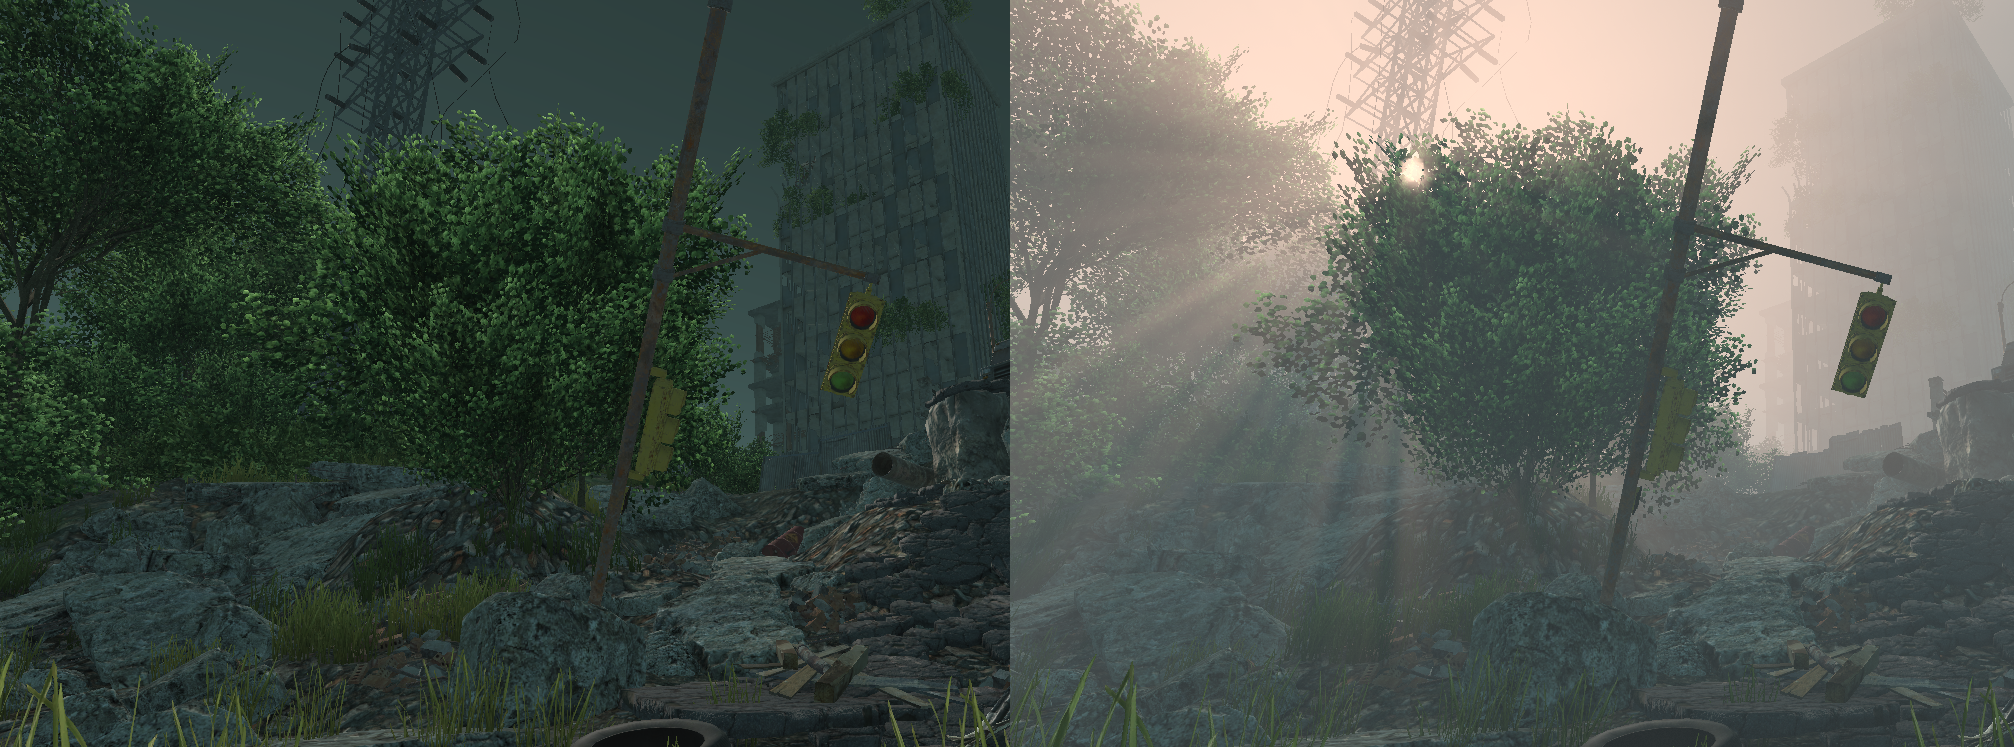
\includegraphics[width=0.8\textwidth]{images/unity-lighting.png}
        \caption{Example of a 3D scene without lighting settings (left) and the same scene with post-processing effects (right). Factors like depth, high-quality volumetric light and fog of variable density allow the construction of realistic environments. Taken from \cite{unity_volumetric_light}.
        }
        \label{fig:unity-light}
\end{figure}

In the setup of a scene, a variety of environment assets such as buildings, trees, rocks, and foliage, are required to convey an authentic depiction of a scene. Sample screenshots of these assets, as well as of the visual effects and skybox assets are illustrated in appendix Figure \ref{fig:assets-unity}. Once all the assets are allocated in a scene, the rendering pipeline can be tuned to adjust the lighting settings to achieve a more realistic rendering if needed. Figure \ref{fig:unity-light} shows the difference lighting makes when simulating a 3D scene, which is one of the many parameters, in addition to color, texture, rotation, position, etc., that can be randomized using a game engine. 
As mentioned in Section \ref{chap2:synthetic-data}, domain randomization allows the creation of a dataset that includes not only corner cases but also allows the learning algorithm to generalize to unseen environments.


Given that the current approach utilizes a grid sensor, octrees and voxels to abstract the 3D environment, the realism of the scene does not play a role in the agent's performance. This setup allows the separation of the 3D modeling work from the agent's algorithm, while still being able to extend to other use cases that can exploit Unity's scripting framework and domain randomization capabilities.



\subsection{Environment Platforms}
An environment platform enables the development, training, and testing of reinforcement learning algorithms. It also provides the necessary interfaces to abstract the interaction between the logic running on a system and the environment that the agent is interacting with.
More concretely, the environment platform provides a variety of features that allow the definition of the state of the game, the actions the agent can perform, the reward functions, and the training strategy. We introduce two environment platforms in the following sections: OpenAI Gym and Unity ML-Agents.

\subsubsection{OpenAI Gym}
OpenAI Gym \cite{github-unity-mlagents-toolkit} is a platform designed to facilitate the development of reinforcement learning agents. OpenAI Gym has been integrated into several popular reinforcement learning systems, including the open-source reinforcement learning platform OpenAI Baselines. Gym supports both training and test modes with a variety of configurations to evaluate and compare algorithms, unifying researchers in reinforcement learning to a common set of interfaces, and abstracts the environment through the \textbf{env} interface. This interface provides the following main abstractions:
\begin{itemize}
    \item \textbf{reset(self).} This resets the environment and returns an observation.
    \item \textbf{step(self, action).} Transitions the environment to state $s_{t+1}$ and returns a tuple of type: \textit{(observation, reward, done, info)}.
    \item \textbf{render(self).} Renders the environment in its current timestep.
\end{itemize}

\subsubsection{Unity ML-Agents}
Unity ML-Agents \cite{github-unity-mlagents-toolkit} is an RL platform which allows the construction of more environments rich in physical and sensory complexity, leveraging the Unity game engine, which is composed of a set of components that enable physics simulations, realistic renderings, etc., as described in Section \ref{chap2:3denvironment}. The platform not only 
provides an abstraction layer for the development of algorithms and sophisticated tasks like autonomous driving, but also supports the development of complex multi-agent applications, curriculum learning, imitation learning, etc \cite{github-unity-mlagents-toolkit}. This is also facilitated given their state-of-the art implementations of algorithms to easily train agents for 2D, 3D, and VR / AR applications. In contrast to OpenAI gym, the ML-Agents toolkit is composed of the following components, illustrated in Figure \ref{fig:unity-learning-environment-full}:

\begin{itemize}
    \item \textbf{Learning Environment.} It encapsules the Unity scene and \textit{game characters}. The Unity scene sets up the environment for the agent to observe, act and learn and has to be modeled and constructed by the developer. The ML-Agents plugin allows the transformation of the scene into a reinforcement learning environment. It uses the Academy component (not illustrated) to ensure that all \textit{Agents} are synchronized and to manage the learning environment's settings.
    % The learning environment through the Academy (not represented in the diagram) ensures that all the Agents are in sync in addition to controlling environment-wide settings.

    % which contains the Unity scene and all the game characters. The Unity scene provides the environment in which agents observe, act, and learn. How you set up the Unity scene to serve as a learning environment really depends on your goal. You may be trying to solve a specific reinforcement learning problem of limited scope, in which case you can use the same scene for both training and for testing trained agents. Or, you may be training agents to operate in a complex game or simulation. In this case, it might be more efficient and practical to create a purpose-built training scene. The ML-Agents Toolkit includes an ML-Agents Unity SDK (com.unity.ml-agents package) that enables you to transform any Unity scene into a learning environment by defining the agents and their behaviors.
    % 
    \item \textbf{Python Low-Level API.}. This is the low-level Python interface which allows communication with a learning environment. This component is separate from Unity, in contrast to the learning environment, and uses the Communicator to interact with the Unity environment.
    
    % which contains a low-level Python interface for interacting and manipulating a learning environment. 
    % Note that, unlike the learning environment, the Python API is not part of Unity, but lives outside and communicates with Unity through the Communicator. 
    % This API is contained in a dedicated mlagents\_envs Python package and is used by the Python training process to communicate with and control the Academy during training. 
    % However, it can be used for other purposes as well. For example, you could use the API to use Unity as the simulation engine for your own machine learning algorithms. See Python API for more information.
    \item \textbf{External Communicator.} This component enables the interaction between the learning environment and the Python Low-Level API.
    % which connects the learning environment with the Python Low-Level API. It lives within the learning environment.
    \item \textbf{Python Trainers.} The trainers contain the machine learning algorithms that realize reinforcement learning. They are implemented in Python and interface through the Python Low-Level API.
    % which contains all the machine learning algorithms that enable training agents. The algorithms are implemented in Python and are part of their own mlagents Python package. The package exposes a single command-line utility mlagents-learn that supports all the training methods and options outlined in this document. The Python Trainers interface solely with the Python Low-Level API.
    \item \textbf{Gym Wrapper.} This component allows the export of learning environments to an OpenAI Gym \cite{github-openai-gym} environment platform. OpenAI Gym is a common platform for developing and comparing reinforcement learning algorithms. 
    % enabling the usage of many different architectures and set ups for training agents. 
    This component is not illustrated. 
    % A common way in which machine learning researchers interact with simulation environments is via a wrapper provided by OpenAI called gym. We provide a gym wrapper in a dedicated gym-unity Python package and instructions for using it with existing machine learning algorithms which utilize gym.

\end{itemize}

\begin{figure}[!ht]
        \centering
        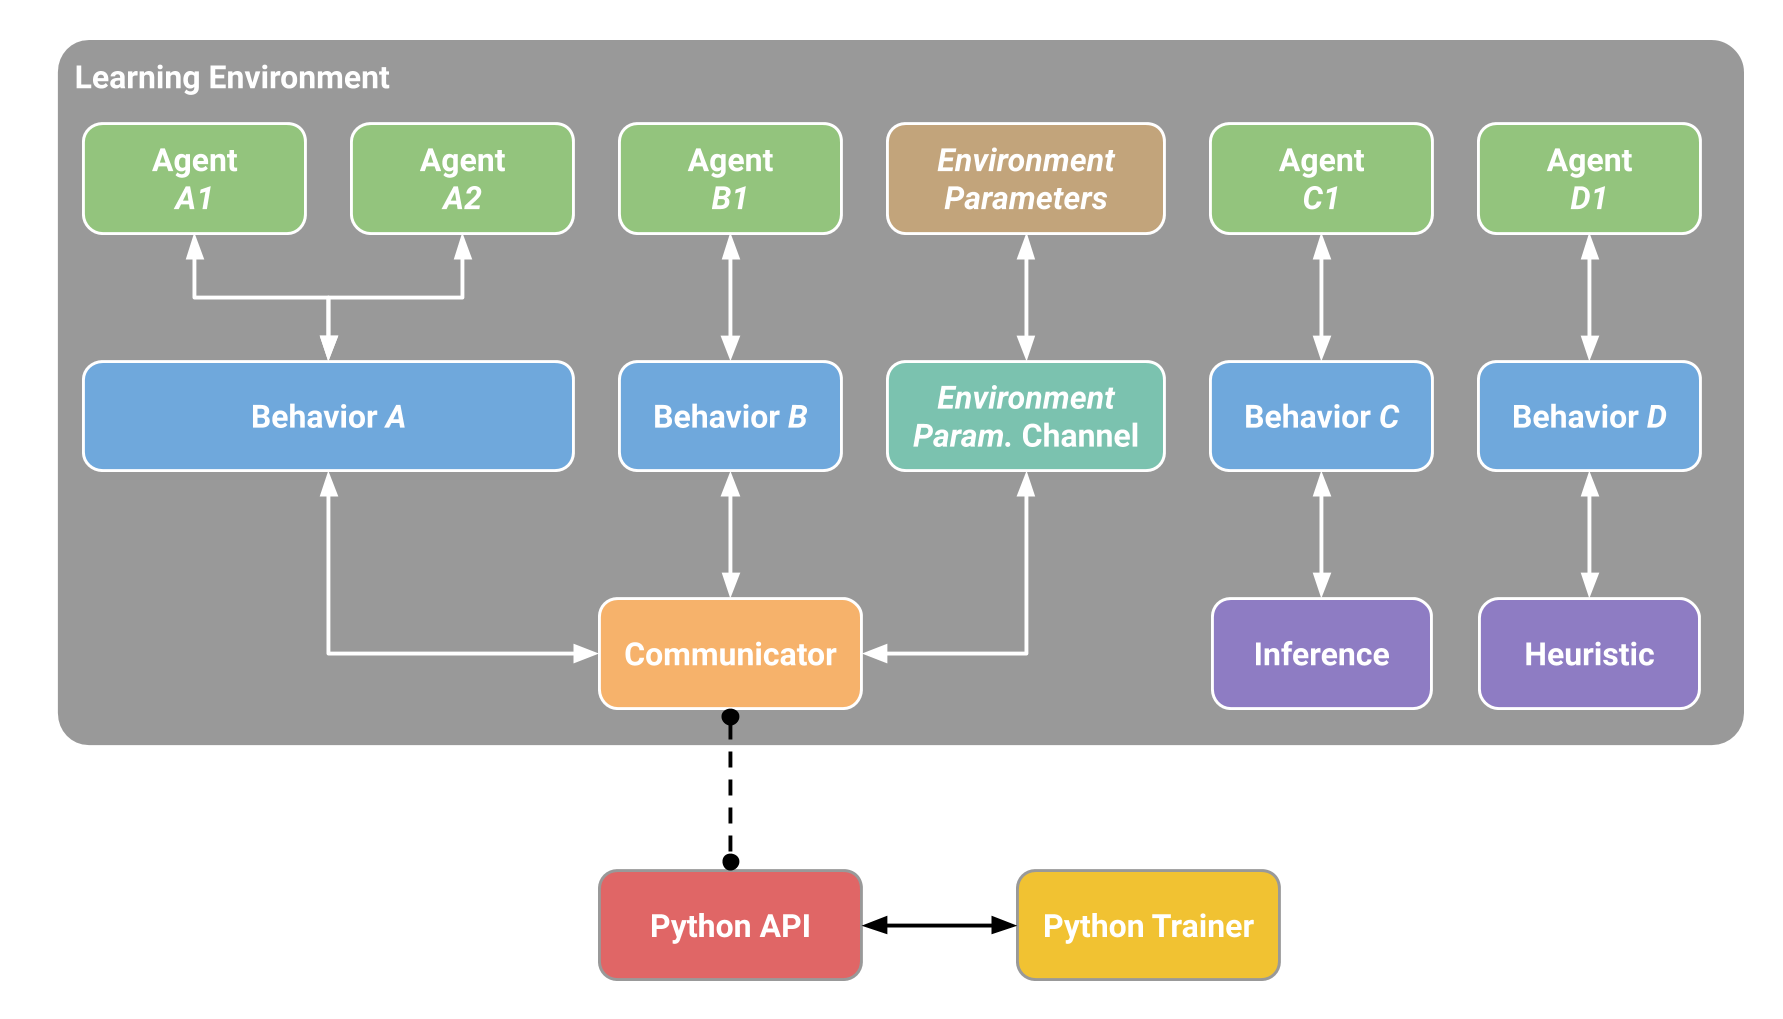
\includegraphics[width=0.96\textwidth]{images/unity-learning_environment_full.png}
        \caption{Overview of the Unity ML-Agents Toolkit, taken from \cite{github-unity-mlagents-toolkit}.
        }
        \label{fig:unity-learning-environment-full}
\end{figure}


Accordingly, the following components in the learning environment aid in the organization of the Unity scene: 
% learning environment
% The learning environment contains two Unity Components that help organize the Unity scene:
\begin{itemize}
    \item \textbf{Agents.} This component abstracts the provision of observations, execution of actions and assignment of rewards and penalties.
    It is attached to a Unity GameObject, which can be any character in the scene, and is linked to a \textit{Behavior}.
    % which is attached to a Unity GameObject (any character within a scene) and handles generating its observations, performing the actions it receives and assigning a reward (positive / negative) when appropriate. Each Agent is linked to a Behavior.
    \item \textbf{Behavior.}. A Behavior component is the logic that takes observations and rewards and returns actions to execute. 
    It also defines the essential characteristics of an agent, such as the type and number of actions the agent can take.
    Finally, it can be of three types: a) a \textit{learning behavior} that communicates that a model should be created and activates the learning process, b) a \textit{heuristic behavior} that limits itself to a set of hard-coded rules for the agent movement, or c) an \textit{inference behavior} that loads a selected learned model and executes the learned policy in the learning environment.
    
    % of the agent.
    % - defines specific attributes of the agent such as the number of actions that agent can take. Each Behavior is uniquely identified by a Behavior Name field. A Behavior can be thought as a function that receives observations and rewards from the Agent and returns actions. 
    
    % A Behavior can be of one of three types: Learning, Heuristic or Inference. A Learning Behavior is one that is not, yet, defined but about to be trained. 
    % A Heuristic Behavior is one that is defined by a hard-coded set of rules implemented in code. An Inference Behavior is one that includes a trained Neural Network file. In essence, after a Learning Behavior is trained, it becomes an Inference Behavior.

\end{itemize}

Every agent in a learning environment will always have an Agent component linked to a Behavior. Similarly, an environment can have a) a single Behavior that can be linked to multiple Agents, as conceptualized in multi-agent scenarios, or b) multiple agents and multiple behaviors. Additionally, it is possible to exchange messages between Unity and Python outside of the reinforcement learning loop using \textit{Side Channels}. 

Moreover, the development of learning environments using Unity ML-Agents plugin also facilitates saving, sharing and synchronizing projects across devices and developers using 
Unity Collaborate \cite{unity-collaborate}.

Finally, Unity 3D was the preferred solution given the aforementioned extensive support toolbox for the development process, intuitive operability, active community, training mechanisms through the Unity ML-Agents plugin, and the capability of extending to future use cases.
% in the construction of Unity scenes to efficiently develop projects in a team of developers.

% Lastly, it is possible to exchange data between Unity and Python outside of the machine learning loop through Side Channels. One example of using Side Channels is to exchange data with Python about Environment Parameters. The following diagram illustrates the above.


% A Behavior will always be present in a learning environment
% Every learning environment will always have one Agent for every character in the scene. While each Agent must be linked to a Behavior, it is possible for Agents that have similar observations and actions to have the same Behavior. In our sample game, we have two teams each with their own medic. Thus we will have two Agents in our learning environment, one for each medic, but both of these medics can have the same Behavior. This does not mean that at each instance they will have identical observation and action values.

% Moreover,
% Note that in a single environment, there can be multiple Agents and multiple Behaviors at the same time. For example, if we expanded our game to include tank driver NPCs, then the Agent attached to those characters cannot share its Behavior with the Agent linked to the medics (medics and drivers have different actions).



\section{Specification of the Perception Approach}
The task at hand requires the agent to be able to perceive its environment. This is done through a set of sensors and techniques that transform the environment from 3D models to some other interpretable form. In our case, this is done through the following:
\begin{itemize}
    \item \textbf{Voxelization} of the objects of interest, which generates an occupancy grid to simplify the shape and structure of the objects.
    \item A \textbf{grid sensor} component, which perceives all the 3D assets environment and feeds visual information to the agent, which is later encoded by a CNN.
    \item \textbf{Octree observations} that provide limited information on how much of the environment has been discovered.
    \item \textbf{Semantic entropy}, which provides information on how many classes are in the agent's field of view over the past few frames.
\end{itemize}
These perceptions mechanisms are presented int he following subsections.

\subsection{Voxelization of the World}
Part of the exploration technique involves providing a way for the agent to investigate objects more exhaustively. Research tends to use RGB(D) images or point clouds for computer vision tasks \cite{xie2020linking, huang2021comprehensive}, which can be both computationally expensive and require a lot of space on memory.
We aim to solve the problem of exhaustive exploration and the drawbacks of 3D data representations through the reduction of data volumes through a voxelized representation. Voxelization models the environment into cubes instead of points, as described in Section \ref{chap2:voxels}. Through the resolution parameter, voxels can largely reduce data volumes with low information loss and minimal overlapping \cite{xie2020linking}. This abstraction of the world is not only useful for visual purposes but also for other tasks, such as navigation and path planning.

% the reduction, therefore enable a reduct complexity reduction the shape and number of cubes in the scene, which allows the reduction of the complexity of the scene through the resolution settings. Th
% for many other things besides vision, such as navigation and path planning \cite{}.

\begin{figure}[!ht]
        \centering
        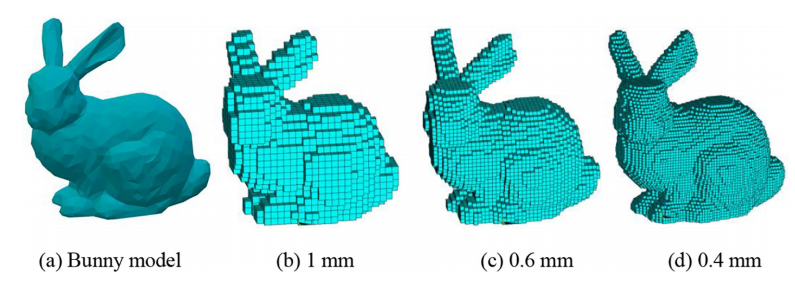
\includegraphics[width=0.7\textwidth]{images/bunny-voxelization.png}
        \caption{Bunny model voxelized at different resolution settings, taken from \cite{zhou2020voxelization}.
        }
        \label{fig:open3D-voxelization}
\end{figure}


Work on voxelized representations of the world have a number of advantages in a variety of use cases that this thesis work is inspired by and takes advantage of, such as as \cite{xie2020linking, zhou2020voxelization, dong2004real, loop2013real, orts2016holoportation}. First, they are space efficient, which makes it easier to store and use a representation of the world, and secondly, since the cubes are a finite volume, they are not restricted by the size of the camera or the resolution of the sensor. Finally, we believe that working with cubes will improve the exploration, because the representation has fewer properties and the agent has more control over the space it perceives. This final property allows the agent to be \textit{visual-agnostic} in the navigation task and understand any kind of environment regardless of the underlying data distribution. This represents a potential bridge for transfer learning tasks for navigation, where the data distribution and preprocessing steps play a critical role in the performance of an algorithm.


In this work, we use an underlying version of a voxelized world, with an isometric representation. The main idea behind voxelization is to represent the world into a medium-sized set of cubes, each representing a specific volume. Each cube can be perceived by the agent and scanned, which awards the agent reward $R^{VOX}$.
% is the first type of reward for our agent. 
There are many methods for efficient voxelization of an environment, as seen in \cite{dong2004real, loop2013real, orts2016holoportation}. For more information on the voxelization process, please refer to Appendix \ref{appendix:unity3d-voxelizing-3dmodels}, which includes the script used to pre-generate a voxelized representation of the 3D assets in the environment.


% \subsection{grid sensors: Vision in the Learning Agent}
\subsection{Grid sensors and Vision from Monocular Cameras}\label{chap:3:gridsensors}
On the topic of vision, panoramic cameras are currently actively used in visual SLAM research given not only their wide range of information perception but also the fast and complete acquisition of information they enable \cite{rill2021collision, wojek2012monocular}.
It is also claimed that spherical cameras will become the norm for driver assistance, traffic safety and autonomous navigation, where visual SLAM techniques must reduce uncertainty as quickly as possible in dynamic environments to prevent collisions \cite{zhang2021panoramic}.
% Recent research \cite{zhang2021panoramic} promotes the usage of monocular cameras as a cheaper alternative to the RGBD variant.



Among monocular cameras, the common camera is less preferred in comparison to other, more expensive alternatives, since it is limited to an angle of view of 60 degrees and a vertical angle of view of 45 degrees. This angle constraints the amount of information fed into the algorithms and adds unnecessary overhead in the feature extraction. More concretely, the extracted feature points to stay in the field of vision for a short period of time, which translates to a different set of challenges and assumptions a technique must take, such as memory, tracking, etc. Accordingly, research by \textcite{davison2007monoslam} highlights that it takes less time to reduce uncertainty and correct positioning errors the longer a feature is observed continuously. For an in-depth review of visual SLAM methods using RGBD and monocular cameras, refer to \cite{taketomi2017visual, zhang2021panoramic}. 



% \begin{figure}[!ht]
%         \centering
%         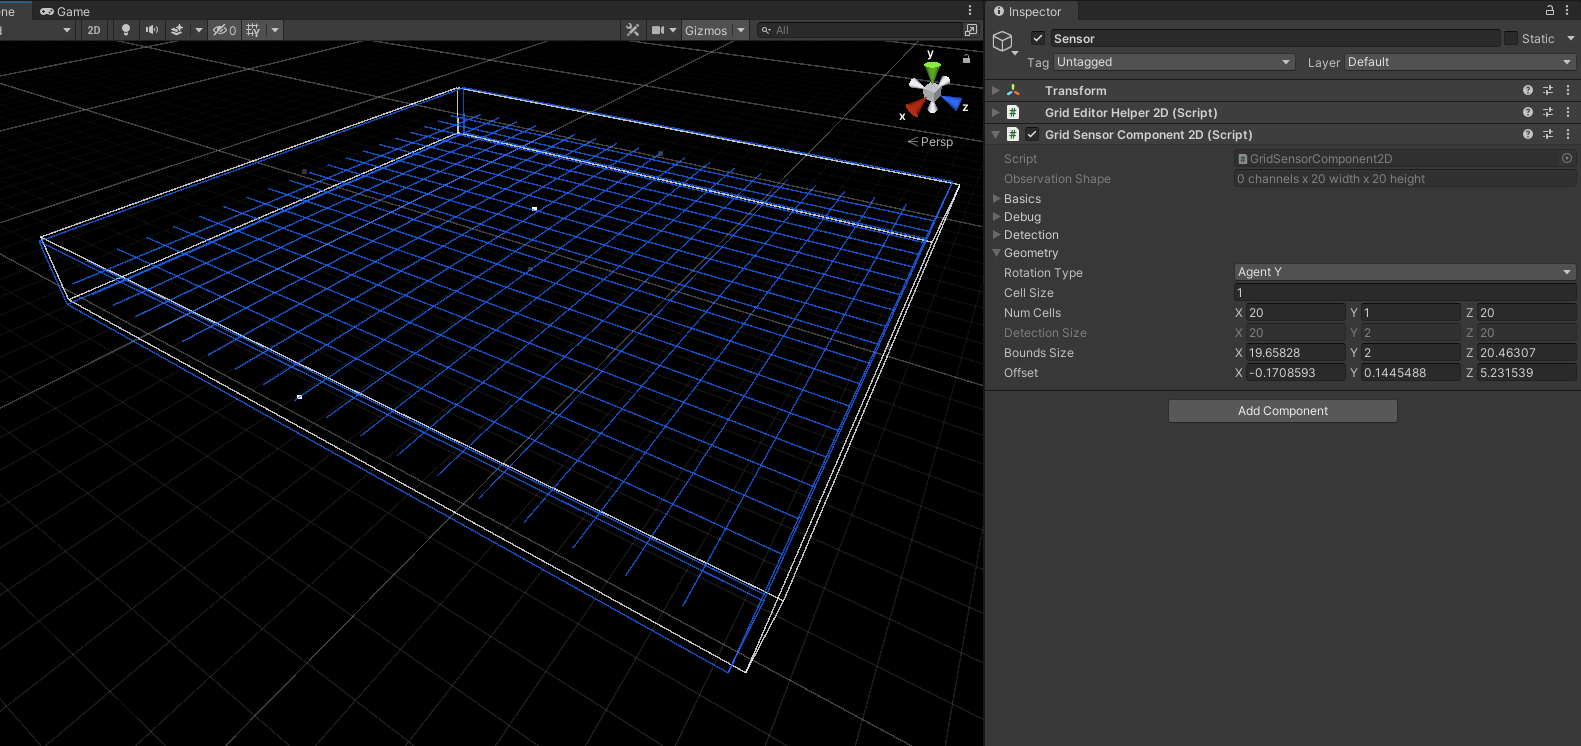
\includegraphics[width=0.8\textwidth]{images/gridsensor-scene-2d.png}
%         \caption{grid sensor 2D \cite{}
%         }
%         \label{fig:gridsensor-2d}
% \end{figure}

% Finally, recent research proves that techniques based on spherical monocular cameras perform better than their limited ordinary variant. 

% Work by \textcite{zhang2021panoramic} provides a thorough explanation of the potential of monocular cameras for the future computer vision research, where SLAM technologies are categorized into LIDAR SLAM and visual SLAM. Even though the LIDAR SLAM has been extensively studied, it remains a more expensive alternative and has a limited range of detection in comparison to camera-based SLAM. As of today, techniques for visual SLAM have used either 1) depth-sensor equipped cameras (RGBD) or 2) monocular, stereo or panoramic cameras. 

% visual SLAM algorithms: a survey from 2010 to 2016
This thesis takes inspiration from these works and the benefits provided by spherical vision, to integrate the agent with a grid sensor component.
The motivation behind using this component roots back to the origins of this component in the reinforcement learning community. 

With the growing interest for reinforcement learning techniques and research, a middle ground was required between model expensiveness and lengthy training times. Moreover, the testing of this middle ground had to be independent of the changing visuals across diverse video games, defined by one of the core principles of Automated Game Testing \cite{unity-eidosmontreal2020}. 
In 2020, the labs at Eidos-Montréal \cite{unity-eidosmontreal2020} innovated the state-of-the-art in perception for reinforcement learning, which at that point was limited to raycasts and cameras, with a simple 2D \textit{grid sensor} component. Inspired by the simplification of an environment in the MinAtar paper \cite{young2019minatar}, the grid sensor exploits the computational efficiency of CNNs with the generality in data structure provided by raycasts. The basic principle behind the grid sensor is to use a height x width x channel matrix of variable resolution, that queries physics information from objects in range. This keeps the spatial structure perceived and can be then fed to a CNN, a reinforcement learning algorithm, or used to perform data analysis. 

% \begin{figure}[!ht]
%         \centering
%         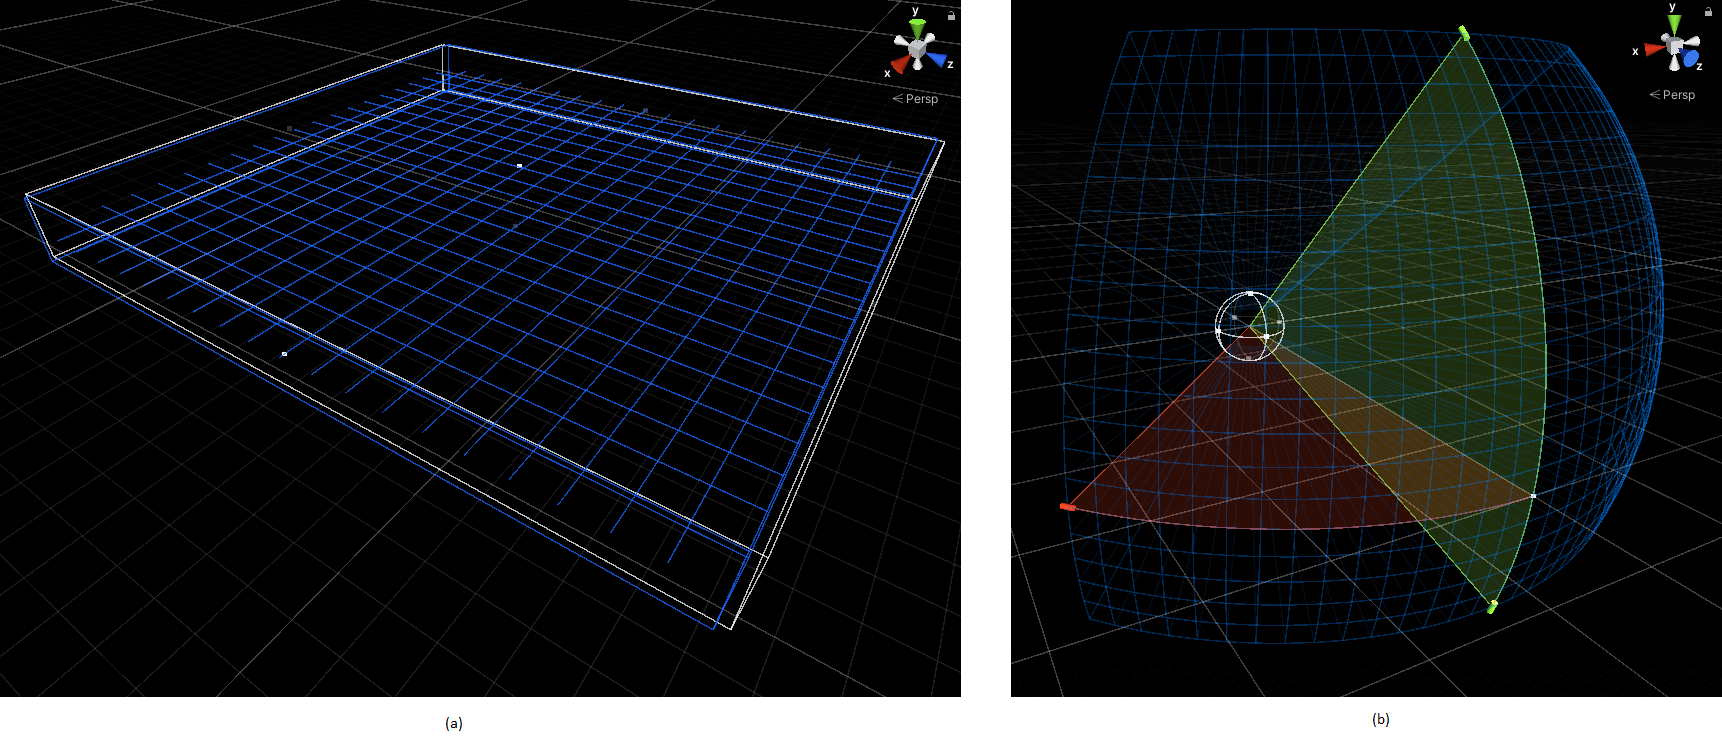
\includegraphics[width=.8\textwidth]{images/gridsensors.png}
%         \caption{Top-down 2D vision and panoramic vision through variants of the grid sensor component for Unity ML-Agents. 2D grid sensor (a) and 3D grid sensor(b), developed by Mbaske \cite{github-mbaske-gridsensor}.
%         }
%         \label{fig:gridsensor-3d}
% \end{figure}


\begin{figure}[!ht]
    \centering
    % \subfigure[]{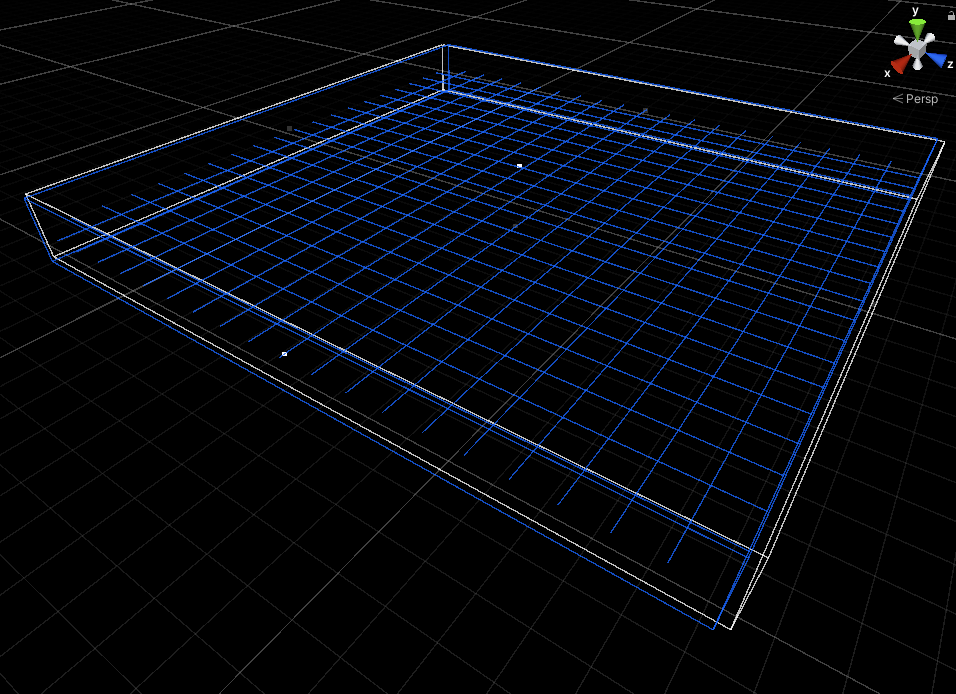
\includegraphics[width=0.538\textwidth]{images/gridsensor_mbaske_2D.png}} 
    \subfigure[]{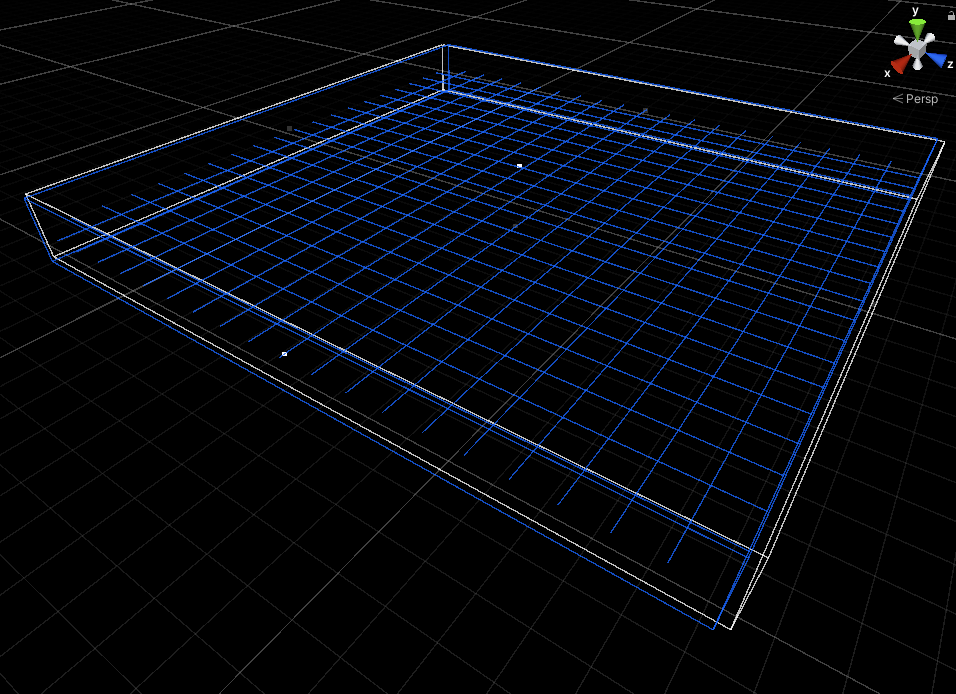
\includegraphics[width=0.4304\textwidth]{images/gridsensor_mbaske_2D.png}} 
    % \subfigure[]{\includegraphics[width=0.40\textwidth]{images/gridsensor_mbaske_3D.png}} 
    \subfigure[]{\includegraphics[width=0.32\textwidth]{images/gridsensor_mbaske_3D.png}} 
        \caption{
            Top-down 2D vision and panoramic vision through variants of the grid sensor component for Unity ML-Agents. (a) 2D grid sensor and (b) 3D grid sensor, developed by Mbaske \cite{github-mbaske-gridsensor}.
        }
        \label{fig:gridsensor-3d}
\end{figure}

The grid sensor used in this thesis is an improved version of the original grid sensor, developed by \textcite{github-mbaske-gridsensor}, under a variety of perception parameters. 
In Chapter \ref{chap:4} we compare the performance of the agent under an ordinary monocular camera setting and a spherical, panoramic, setup. 
This, in conjunction with a voxelized representation of the world, conceives a training agent that is input-agnostic and can greatly increase the training time in 3D environments. 
Since this setup does not depend on the rendering of visuals, training in the configuration file can be set to headless mode, which means that it runs as a normal computer process but no GUI is shown in the computer screen. This allows the agent to train while still using high-dimensional data and the benefits of domain randomization, such as position and domain randomization. Moreover, the 3D creative process involving textures and lighting setup is completely detached from the agent's behavior training setup. 
Our aim is that this also motivates further research in reinforcement learning to enable transfer learning of agent behaviors from training in simple environments to progressively more complex ones. 
The grid sensor developed by Baske can be found at \url{https://github.com/mbaske/grid-sensor}, and is visualized in Figure \ref{fig:gridsensor-3d}. 


% . There is extensive research into LIDAR SLAM in com 
% Panoramic Visual SLAM Technology for Spherical Images
% It refers to the use of a sensor in an
% unfamiliar environment, where the data observed by the sensor are used to estimate the
% state of motion of the sensor itself, while building a map of the surrounding environment.
% SLAM technology can be divided into LiDAR SLAM and visual SLAM. For historical
% reasons, the research into LiDAR SLAM began earlier than research into visual SLAM,
% and LiDAR SLAM technology is more mature than visual SLAM technology in theory,
% algorithms, and landing products. However, LiDAR is more expensive than cameras,
% and LiDAR has a limited range of detection. Cameras have no distance limit and cost
% less. 
% At present, the solutions for visual SLAM technology are mainly based on RGB-D
% cameras and monocular, stereo, or panoramic cameras. The biggest difference between the
% two schemes is that RGB-D cameras are equipped with depth sensors, whereas ordinary
% monocular, stereo, and panoramic cameras are not. Since RGB-D cameras are generally
% more expensive than ordinary cameras, it is of great significance to study visual SLAM
% technology based on ordinary cameras (like monocular, stereo, or panoramic cameras without depth sensors), to reduce the cost. 
% Among the ordinary cameras, panoramic cameras
% have gradually become one of the hotspots in the field of visual SLAM research because of
% their wide range of information perception and fast and complete information acquisition.

% https://link.springer.com/content/pdf/10.1007/s42979-021-00759-6.pdf
% In contrast to regular cameras which can monitor one view at a time, research suggests spherical monocular cameras will become the norm in autonomous driving applications.

% \textbf{Applications of Monocular Videos.}
a 
% Research by 

% Autonomous driving methods have shown impressive results based on monocular vision. 
% Methods calculate the time-to-collision method based on monocular depth. 
% http://stanford.edu/class/ee367/Winter2020/report/lee_hong_lee_report.pdf
% https://www.mpi-inf.mpg.de/news/spotlights/understanding-images-videos/3d-scene-understanding-from-monocular-cameras
% new

\subsection{Navigation with Octrees}
\begin{figure}[!ht]
        \centering
        \includegraphics[width=0.5\textwidth]{images/octree-explorer-drone.png}
        \caption{Octree Construction and Navigation in Mbaske's Explorer Drone \cite{github-mbaske-explorer-drone}.
        }
        \label{fig:gridsensor-3d}
\end{figure}

As described in Section \ref{chap2:octrees}, octrees can be used to subdivide a scene in hierarchical nodes, providing a  way to efficiently deal with large amounts of space. Since our application of octrees is not meant for rendering, the drawbacks of octrees in comparison to polygons can be disregarded. 
On every step, the agent adds new nodes to the octree, which can be of three types: empty nodes (scan out of range), point (scan) nodes, and nodes that have been visited.
Information about the octree is part of the agent's observations, presented in Section \ref{chap:3:agent-choice-actions}.
The reward $R^{OCT}$ is part of the reward signal the agent receives, and it is proportional to the number of new nodes added to the octree. The reward is further defined below in Section \ref{chap:3:reward-signal}.
The implementation of octrees for Unity was taken from Baske's Explorer Drone, which can be found at \cite{github-mbaske-gridsensor}.
% here: \url{https://github.com/mbaske/ml-explorer-drone/blob/master/UnityEnv/Assets/Drone/Scripts/Octree.cs}. 

% which in our setup can be leveraged to motivate agent exploration through the addition of nodes.

% The benefits of octrees are that they give us a way to efficiently deal with large
% amounts of data and that they can be used to implement ray tracing, which is
% important for many real time applications. A
% n octree consists of a data structure
% that allows us to store data in hierarchal nodes. These nodes can be described
% as cubes and spheres in 3D space or as octagons in 2D space. The basic idea behind
% an octree is to divide a given space into a set of small cells and then to build
% a data structure that allows us to efficiently access to the contents of those cells.
% Once a space has been divided

% The disadvantages of using octrees are the overhead and memory usage associated with them. A simple octree has to store for each face (not to forget the 8 corner nodes) 8 3D vector points, and this is the worst case because most faces are triangles, but not necessarily all of them. An octree can contain between 8-32 or even 64 triangles. A simple octree is also limited to 3D vector input, not 4D tensor input. The octree can be limited in other ways (for example the octree has to be static and can be very big).


% This box representation provides some advantages for many applications, as is shown in Section \ref{octree_section}. 
% There are however some trade-offs between the complexity and size of an octree compared to that of a set of polygons. 
% % (see Table \ref{octree_table}). 
% A set of polygons can represent the same area as an octree with roughly half the number of boxes, with the advantage of being simpler to create and maintain.

% The implementation of an octree in a graphics application is beyond the scope of this paper, however there are several resources available to the interested reader, including \cite{Octree}, \cite{Octree2D}, and \cite{OctreeSectional}. We use the \cite{Octree} implementation for our work in this paper.

% At the start of the exploration process, we initialize an octree and create some random objects and their bounds. We will use this tree to represent the area of the scene the agent is currently exploring, along with any objects or bounding boxes that are inside that area. After an initial exploratory action, we then explore one area at a time by selecting the nearest neighbour of the last explored area. In our implementation, we use a greedy selection procedure, where we calculate the average distance from all objects to all other objects and then select the object with the minimum average distance. The process is repeated for each of the areas on the tree.


% This section presents the chosen definition of uncertainty or uninformativeness in an environment.

% \textbf{System Entropy.}
% In physics, entropy is defined as 

% n physics, entropy is a measure of the degree of "disorder" in a physical system. It is defined by the relation between the system's energy (work) and the system's capacity for transformation (free energy, free capacity, free energy). The entropy of an isolated system never changes. 
% entropy is used to measure the uncertainty associated with the distribution of outcomes from an experiment or a random variable. 
% In information theory, inconsistency is denoted as entropy, where entropy is a function of probability distribution functions (pdf's). If P is a pdf over the random variable X, then the entropy of P is defined as:

\subsection{Semantic Entropy}\label{chap:3:semantic-entropy}
In 1997, \textcite{melamed1997measuring} defined semantic entropy as a way to measure semantic ambiguity, uninformativeness or as the inverse of semantic reliability. In this thesis, we are especially interested in the concept of entropy as the degree of randomness or disorder in an environment, in line with the definition given in information theory, which defines entropy formally as
\begin{align*}
    H(X) = - \sum_{x\in X} P(x_i) log P(x_i).
\end{align*}
where $X$ is a discrete random variable, with possible outcomes $x_i$ and $P(x_i)$ is the probability that outcome $x_i$ occurs.

Heavily inspired by recent work on exploration by \textcite{chen2019learning} and  \textcite{chaplot2020semantic}, and as part of the answer to the research questions, we leverage the concept of entropy to define the uncertainty in an environment or a 3D object. \textcite{chaplot2020semantic} utilize semantic curiosity to learn exploration trajectories based on semantic maps. These semantic maps contain information about the inconsistency provided by an object detector at position $P$, and are used as a motivation for a reinforcement learning agent to prefer states with higher entropy. In their words, "if an object is labeled with different classes as the viewport changes, it will have high temporal entropy". Similarly, this thesis constructs a short-term memory buffer that measures the temporal inconsistencies perceived by an object detector as a way to measure semantic entropy in the agents field-of-vision. This metric, in contrast to the semantic curiosity motivation, is used to influence the linger estimator in the agent. More concretely, it acts as a discount factor in the definition of the penalty given by inactivity. The definition of the reward signal is presented in Section \ref{chap:3:reward-signal} below.



% \textbf{Reliability through Object Detection.}



% The agent started at a random location in the environment and had to navigate and reach a target location by a sequence of movements. After reaching the target location, the agent continued to move in the environment until it was back at its starting location.



% Also, under the current project's conditions it is not viable to manually annotate a point cloud. 
% It is also unfeasible to load a batch of point clouds into memory for training. Given the lack of additional inputs, each entry of the data set contains:
% \begin{itemize}
%     \item RGB image of the cow teats.
%     \item Pixel-wise segmentation mask, labeling the locations of the cow teats in the RGB image.
% \end{itemize}
% The nature of the data was two fold: synthetic and realistic. The collection of the realistic data was done at a laboratory at the ZHAW. Given the limitations of the first iteration of the milking robot project, the collection of real cow images was not required. The environment setup and details of the training data collection are described in Chapter \ref{chap:evaluation}. Finally, even though the images collected from the camera could be directly used for training, the preprocessing required was the adaptation of the data set to the COCO data format. Once formatted, the neural network could be trained.

% Consequently, the collection of the synthetic data was done using Unreal Engine 4 and a plugin from NVIDIA \cite{2021ue4} called NDDS \cite{2021ndds}. Photorealistic scenes are created in Unreal Engine 4 and NDDS allows for the annotation of objects in UE4. These scenes are then exported and all the information from the objects is included in the export, such as objects, classes and 3D poses. Additionally, the export includes the respective rgb image, depth image, instance segmentations and class segmentations for the frame taken. Appendix \ref{appendix:ndds} illustrates a 3D scene and an export sample.

% Even though the implementation computer vision pipeline required to generate voxels is out of scope for this work, we describe briefly the steps required to obtain the resulting 3D representations from RGBD images in Figure X. Captured RGBD images from a camera can be transformed into point clouds using Open3D's method 



% As described in Section \ref{chap:2:segment}, object segmentation involves the pixel-wise assignment of labels in an image that belong to a specific class. The following techniques were considered suitable for this task:
% \begin{itemize}
%     \item \textbf{Recognition of Fixed Shapes} A set of features are generated from the geometric information, such as 3D points, lines or surfaces. These features are then matched to a predefined model features. If the similarity evaluation between the model and the detected features is sufficient, a frame transformation is executed to identify the pose of the detected object. This pose detection represents a hypothesis, among many other hypothesis which are generated while evaluating, for example, a point cloud. Therefore, an appropriate criteria must be used to determine if the hypothesis should be accepted or rejected (hypothesis evaluation). An alternative approach consists of single generating descriptor features from clusters generated in a scene for posterior matching.
%     \begin{description}
%     \item \textbf{Algorithm Used: } RANSAC \cite{2021scikit-ransac}.
%     \end{description}
    
%     \item \textbf{Recognition of Object Classes} An algorithm is used to recover a 3D model from the input (image or point cloud), which is then segmented and then classified. Methods like an RDF classifier or CNNs can be used for classification. Then, methods like surface-to-surface distance minimization are used to retrieve the best match. Both realistic and synthetic RGB-D data sets have been published over the past few years for training and testing RGB-D algorithms. Furthermore, it is important that these methods are able to infer the complete 3D shape from a single frame, specially for robotic tasks like grasping.
%     \begin{description}
%     \item \textbf{Algorithm Used: } DOPE \cite{tremblay2018deep}.
%     % \item \textbf{Algorithm Used: } 

%     \end{description}
    
%     \item \textbf{Feature-based Recognition} Similarly to the recognition of fixed shapes, a set of 3D descriptor features are generated from the geometric information (keypoints) and then evaluated. These descriptor features can be defined by a set of  parameters, such as point coordinates unit vector orientations, point feature histograms of the local surface properties (PFH), etc. A major advantage of these methods is that they require only a single correct feature correspondence to recognize an object.
%     \begin{description}
%     \item \textbf{Algorithm Used: } Manual Manipulation "MAV". This algorithm leverages the segmentation mask and overlays it over the depth image. Afterwards, the 2D points are proyected into 3D space and PCA is used to calculate the teat direction. Finally, the N points (averaging method) at the bottom of the teat (using the direction indicated by PCA's first component) are averaged to obtain a "teat's tip coordinates". A manual offset was added to the obtained coordinates to attempt to fix the (x,y,z) error observed.
%     \end{description}
    
% \end{itemize}

% For each of the methods described above implementations were chosen to predict based on the data sets.  It is important, during the construction and training of a classifier, to tune the parameters of each model. On one hand, for the object segmentation approach, the parameters that were tuned were the learning rate, the score threshold for prediction, the number of workers, the number of iterations, the images per batch and the batch size. On the other hand, for the pose estimation approaches many parameters were tuned, specific to the method, such as maximum number of cow teats in memory, memory tracking reset conditions, frame transformations, etc.

% There were several challenges faced during this phase. Both synthetic and realistic data sets were used for validating not only the models but also the data sets. It was observed that 1) some implementations of the segmentation network used were slower than the final implementation used and 2) the synthetic data set was too different and the reality gap could not be closed. Additionally, allocating resources in the CPU posed a problem in the diverse training and testing. This could be solved by allocating resources in a remote GPU cluster, but set different kind of limitations in the development process.  Finally, due to the fact that many algorithms were tested, the architecture's base concept was a modular design with a plug-and-play approach.

% \section{Agent Setup}
% Once the 3D environment is constructed, the next step is to layout the capabilities of the agent. This section describes the 

\section{Specification of the Agent Character}

% The next step is the modelling and simulation of the learning agent. 
An agent is simulated through 3D assets, observations collected from an environment, actions, movement algorithms and a policy that motivates a specific behavior. The following sections provide insight into these key areas.
Furthermore, our proposal agent behavior the exploration task, is the result of a hierarchical composition of behaviors, as illustrated in Figure \ref{fig:baselines_hierarchical}. This composition starts with a base DroneAgent, that sets the basic requirements for any other agent, which includes movement, sensing and interaction. Posterior layers provide additional logic to train specific policies. For example, the \textit{SpeedDrone} takes into account variables such as angular speed, forward velocity, etc., to train an agent to  minimize the speed error between its current speed and a target speed. The same logic follows for other agents such as the OctreeAgent, VoxelAgent, ShortestPathAgent, etc., where observations that belong to the specific domain of the policy to be trained are added on top of previous layers. More detail on the hierarchical construction of these agents can be found on Appendix \ref{appendix:baselines}.

\begin{figure}[!ht]
        \centering
        \includegraphics[width=0.7\textwidth]{images/baselines_hierarchical_construction.png}
        \caption{Hierarchical construction of the agent behaviors in Unity. The DroneAgent contains embodiment logic of the agent such as relative position and orientation. Higher behaviors inherit from the DroneAgent and implement speed, perception of octree nodes, perception of voxels, detections from a YOLO classifier, etc. 
        }
        \label{fig:bselines_hierarchical}
\end{figure}

Given that the base drone lays the ground logic for the rest of the agents, a brief explanation of its components is due. The base agent layer introduces 
\begin{itemize}
    \item A 3D model of an agent.
    \item A movement algorithm.
    \item Basic information for embodiment such as such as agent's position, rotation, its velocity, etc. 
    \item A grid sensor to enable perception of the environment, as introduced in Section \ref{chap:3:gridsensors}.  
    \item A scanner component, which enables interaction with the voxels in the environment.
    \item A reward signal.
    \item An episode reset logic.
\end{itemize}

Given that the base layer provides the foundation for other derived agent behaviors, the aformentioned elements are described in more detail in the sections below.

Similarly, the base agent allows the introduction, implementation and testing of:
 
\begin{itemize}
    \item a modeled 3D environment.
    \item an environment and goals controller. 
    \item the diverse environment platform components, described in section.
\end{itemize}
An environment and goals controller, also known as the \textit{TrainingAreaController}, looks into the randomization of the environment obstacles, goals and initializes the necessary variables for the agent’s future episode.


% % As mentioned, the base agent encompasses the necessary logic and elements required for movement, and sensing and interacting with the environment. This layer introduces the following:
% \begin{itemize}
%     \item \textbf{Basic information} is collected such as agent's position, rotation, its velocity, etc.
%     \item \textbf{Perception} is done through a grid sensor component, which was introduced in Section.
%     \item \textbf{Interaction} with the environment happens through a scanner component which allows the agent to scan voxels that fall into the constraints set, such as maximum scan distance, angle and resolution.
%     \item \textbf{Movement} is enabled thanks to a CharacterController component in two modes: translation- and physics-based. These modes are described further below.
% \end{itemize}

Consequently, composed agent behaviors follow the structure described for the base agent and incrementally add observations  and reward signals to motivate learning a different policy. In our case, the exploratory behavior is achieved thanks to the policy provided by the OctreeAgent's behavior and the policy that motivated in-depth scanning of objects is given by the VoxelAgent's behavior. More detail is provided for each derivative agent in tables \ref{appendix:baselines_observations, appendix:baselines_rewards}.


\subsubsection{3D Models}
The 3D models for the agent were obtained from the Unity Asset Store \cite{unity-asset-store} and Sketchfab \cite{sketchfab2021} as potential avatars for the learning agent in different scenarios. Figure \ref{fig:unity-drone} visualizes some models considered for the agent, where the Drone Bot was the chosen model, given the overhead complexity of animating the rigs of the other 3D models. To make the simulation more realistic, the drone was given a set of animations, volumetric lights and particle systems.

\begin{figure}[!ht]
    \centering
    \subfigure[]{\includegraphics[width=0.24\textwidth]{images/unity-assets-spot.png}} 
    \subfigure[]{\includegraphics[width=0.24\textwidth]{images/unity-assets-dronebot.png}} 
    \subfigure[]{\includegraphics[width=0.24\textwidth]{images/unity-assets-teslabot.png}}
    \subfigure[]{\includegraphics[width=0.24\textwidth]{images/unity-assets-wireframe.png}}
    \caption{Learning agent 3D model candidates: (a) Spot Bot, (b) Drone Bot, (c) Tesla Bot. (d) Wireframe Shader used for visualization of voxel scanning. Taken from \cite{unity-asset-store, sketchfab2021}.}
    \label{fig:unity-drone}
\end{figure}

\subsubsection{Scanner}
% affect the state of the objects around him. 
The scanner component allows the agent to scan voxels perceived from the environment given a set of constraints such as minimum angle and distance. It is made visible to a human spectator in the graphical user interface through a a special VFX feature of Unity's render engine, namely the \textit{wireframe shader} \cite{unity-asset-store}, which is displayed in Figure \ref{fig:unity-drone} (d). This shader, with the support of an invisible cone \textit{collider} \cite{unity2021} in the scanner component, modifies the render effect of the textures of objects, and displays a wireframe of the object's mesh in the intersection between the scanner's cone collider and the object's collider.

\subsubsection{Movement Algorithms}
To provide actions to the agent, i.e., to simulate a real world robot, the key challenge was the mobility algorithm for the agent. In this work, the agent was given the capability of moving in a three-dimensional environment, so it would be able of reaching any desired location.
To this end, two mobility algorithms were implemented:
\begin{itemize}
    \item Translations-based movement with a rotating function.
    \item Physics-based movement.
\end{itemize}
The simpler variant was implemented using 3D translations, applied to the agent transform's local coordinate system.
The second variant of the mobility algorithm was inspired by the movement model of a real robot, considering concepts such as velocity, torque and motor noise. Both approaches allow the robot to navigate its environment without the help of an explicit movement model.

\textbf{Physics-based movement.}
This algorithm can be defined as:
\begin{align*}
    v_t = v_t + i_t * \eta_1
\end{align*}
and
\begin{align*}
    \tau_t = \tau_t + \mu * clip(turn_t * \beta, -1, 1) * \eta_2
    % Vector3(0, 1, 0)
\end{align*}
where $v_t$ is the agent's rigidbody velocity at timestep $t$, which receives a velocity change force based on input $i_t$ at timestep $t$. This input consists of a \textit{forward input}, a \textit{vertical input}, and a \textit{lateral input}. This force is constrained by a movement speed parameter $\eta_1$, measured in meters/second. Similarly, $\tau_t$ is the rigidbody's torque at timestep $t$ which is increased by a vertical unit vector $\mu$ times the turn input $turn_t$ received at timestep $t$. The turn input is clipped to limit the possible rotation at each timestep by the agent, and is constrained by a turning speed parameter $\eta_2$.

\textbf{Translation-based movement.}
This algorithm can be defined as:
\begin{align*}
    x_t = translate(i_{xt}, i_{yt}, i_{zt}) * \eta_1
\end{align*}
and
\begin{align*}
    r_t = rotate(\mu, clip(turn_t * \beta, -1, 1) * \eta_2 * \Delta t
\end{align*}
where $x_t$ is the agent's position in the 3D space at timestep $t$, which is moved or translated based on the decomposition of the inputs received at each axis. A translation moves an object in the direction indicated by its transform's local axes. Each component from $i_t$ is previously constrained by a movement speed parameter $\eta$, measured in meters/second and regulated for smooth transitions by a time variance parameter $\Delta t$. 
Similarly, $r_t$ is the transform's rotation of the agent at timestep $t$ which is rotated by the game engine given a vertical unit vector and the turn input provided by the agent. As with the physics-based algorithm, the turn input is clipped to limit the possible rotation at each timestep. It is also constrained by a turning speed parameter $\eta_2$ and regulated by a time variance parameter $\Delta t$ to allow smooth rotations in the game engine.


\subsubsection{Additional components} 
Finally, collision parameters were also considered in the modeling of both the agent and the environment to enable the detection and avoidance of obstacles.
Therefore, the learning agent consists of the following components:
\begin{itemize}
    \item A mesh renderer that allows the visualization of the textures from the chosen 3D model.
    \item A physical body which includes a capsule collider and rigidbody components.
    \item A character controller script that captures and reacts to the input, according to the chosen mobility algorithm.
    \item An agent controller script, which is required to use the Unity \textit{ML-Agents} plugin.
\end{itemize}

The agent is therefore defined by a set of components, observations, and parameters that enable perception of both the environment and itself. 
Firstly, the components included in the agent are a 3D and a 2D grid sensor, enabling a visual input of the environment. 
Secondly, the metrics that the agent can perceive include its position, velocity, direction towards goals, etc., which register the metrics of its own rigidbody and of the objects in the environment. Finally, additional parameters such as visibility constraints, scan speed constraints and sensor noise allow the agent to learn to adapt different settings and variability configurations.
The choice of agent observations is described in the next section.
% variables that define the agent's observations can be found below in Section \ref{chap:3:agent-choice-actions}.

% are further described in the sections below. Similarly,  in sections \ref{chap:3:specification-approach} and \ref{chap:3:experiments}.




\section{Specification of the Reinforcement Learning Approach}\label{chap:3:specification-approach}

This section describes selection of a set of reinforcement learning baselines to compare our method to the choice of agent observations for the learning algorithm and the actual processing step. The following questions will be answered in this section:
\begin{itemize}
    % \item Which observations were considered for the exploration task?
    \item What reinforcement algorithm was chosen for the exploration task?
    % \item Which and how many approaches were considered appropriate for the exploration task?
    \item How was the exploration approach implemented (high-level)?
    \item What optimization steps were taken in the algorithm?
    \item What were the main problems found during this phase?
\end{itemize}

% A trade-off between machine learning techniques is always involved when comparing the advantages and disadvantages of each approach. Therefore, a variety of approaches were considered for the mentioned tasks, evaluated and optimized.


% Markov Decision Process refers to the fact that the system obeys the Markov property:
% which indicates that transitions only depend on the most recent state and action, and no
% prior history, in other words, the future is conditionally independent of the past given
% the present state. p (st+1|s1, a1, . . . ,st, at) = p (st+1|st, at)

% \subsection{Agent}


% As described in Section \ref{chap:2:segment}, object segmentation involves the pixel-wise assignment of labels in an image that belong to a specific class. The following techniques were considered suitable for this task:
% \begin{itemize}
%     \item \textbf{Random action sampling} 
%     \item \textbf{Q-learning} A K number of clusters is given to divide the data in to K groups or clusters, based on similarity.
%     \item \textbf{PPO} A histogram is used to group pixels based on gray levels, where the background is one big peak and then the other "hills" are objects.
%     \item \textbf{SAC} A histogram is used to group pixels based on gray levels, where the background is one big peak and then the other "hills" are objects.
%     \item \textbf{Curiosity} Changes in brightness are identified using filters to locate edges, curves and shapes. 
%     \item \textbf{Imitation Learning} As described in Section \ref{chap:2:segment}, convolutional operations are used to label the pixels. This approach scans the image by segments, for example using a sliding windows approach.
%     \item \textbf{Multi-Agent Environments} Contrary to to CNNs, FCNs can take different kinds of input, and output a matrix of dimensions H x W x C (image height, image width, number of classes).  
% \end{itemize}
% Among all the suitable methods tested, the segmentation problem was best tackled using two implementations of MaskRCNN: matterport/MaskRCNN and Detectron2 (FacebookAI). The evaluation and performance of both approaches is described in Section 5.

% Approaches out of scope using images are discarded given the overhead in training times given the 
% latency of images. algorithm itself would reach a similar performance just in a longer time.

% In the evaluation of the each policy, a variety set of hyper-parameters were also tested such as the extrinsic reward rate, curiosity, batch size, horizon, 

Among the multitude of reinforcement learning methods, this thesis work uses Proximal Policy Optimization (PPO), which was presented in Section \ref{chap2:ppo}. This algorithm was chosen given its demonstrated performance in a variety of tasks \cite{berner2019dota, akkaya2019solving, schulman2017proximal, yu2021surprising}, its simplicity compared to other implementations \cite{schulman2017proximal}, and general robustness. A robust algorithm shows stable performance without high dependency on hyperparameter tuning procedures or hyperparameter searches \cite{schulman2017proximal}.

The neural network used is an implementation of the original by \textcite{schulman2017proximal} taken from \cite{github-unity-mlagents-toolkit}, and it is composed of two hidden layers where the number of hidden units is part of the hyperparameter tuning process. 
This network was chosen given its demonstrated performance in \cite{mnih2015human, kempka2016vizdoom, lample2017playing}, sample efficiency in comparison with other off-policy methods \cite{yu2021surprising}, and the added benefit that its reduced size allows faster training times.
PPO requires the approximation of both the state-value function and the policy, which can be done with a shared-parameter network with two heads or two separate networks. We have opted for a shared-parameter network as in the original work by \cite{schulman2017proximal}. 

\begin{figure}[!ht]
        \centering
        \includegraphics[width=1\textwidth]{images/PPO-unity (1).png}
        \caption{Overview of the PPO Trainer's workflow from Unity ML-Agents. Figure adapted from \cite{github-unity-mlagents-toolkit}.
        }
        \label{fig:unity-drone}
\end{figure}

The workflow for each trainer is presented in Figure \ref{fig:unity-drone}, using Unity ML-Agents \cite{github-unity-mlagents-toolkit} as the target platform. The development of the scenes and training of the agent was performed on a Windows 11 machine with an Intel i7-8700k CPU and 32GB RAM.
% and training process 
% Figure {} presents an overview of the PPO trainer from ML-Agents. 
The trainer can receive both visual observations, such as camera, raycasts, grid sensor inputs, and vector observations. Vector observations are any attribute set to observe, such as position, velocity, number of nodes in octree. Additionally, the visual encoder that receives the visual observations can easily be swapped for one of the following: 
\begin{itemize}
    \item A simple encoder with two convolutional layers.
    \item A CNN implementation by \textcite{mnih2016asynchronous}, which contains three convolutional layers.
    \item The IMPALA ResNet \cite{espeholt2018impala}, which has three stacked layers, each with two residual blocks.
    \item The "match3" CNN by \textcite{gudmundsson2018human}.
    \item A single fully connected dense layer.
\end{itemize}

Similarly, capabilities such as attention, LSTM, curriculum learning, multi-agent setups and more can be easily changed or added in Unity to construct an agent for a variety of practical reinforcement learning scenarios \cite{github-unity-mlagents-toolkit}. Figure \ref{fig:unity-simple-encoder} presents an example of the visual encoders mentioned.
% For more information on the visual encoders, please refer to Appendix \ref{appendix:visual-encoders}.

The main challenge during this stage was the delay introduced by training a reinforcement learning algorithm, where observations are provided but the performance cannot be estimated until the agent has been trained. Hence, a method with good sample efficiency was also an important factor that was considered when PPO was chosen.


\begin{figure}[!ht]
        \centering
        \includegraphics[width=0.8\textwidth]{images/simple_encoder.png}
        \caption{Visual encoder example, architecture by Mnih et al. Figure adapted from \cite{mnih2016asynchronous, github-unity-mlagents-toolkit}.
        }
        \label{fig:unity-simple-encoder}
\end{figure}

% \begin{longtable}{@{} p{3.5cm} p{4cm} p{4cm} @{}} \toprule
% \textbf{Layer}       & \textbf{Hidden Layer 1} & \textbf{Hidden Layer 1} \\ \midrule
% Input                &  128 & 128 \\ \cmidrule{1-2}
% Output           & An image exists. \\ 
% Activation           & An image exists. \\ 
%                         & ROSTeat node is running. \\ \cmidrule{1-2} 
% Exceptions             & Image is not RGB \\ \bottomrule
% \caption{Use Case - Predict Masks} \label{tab:use-segment} \\
% \end{longtable}





% and always converges

% This network design is quite
% small, and using a small network was a conscious choice since network size affects
% training times. 

% The network design was deemed suitable since there exists other
% image-based agents that use networks of similar size and design [10–12]. 

% In PPO,
% both the value function and policy need to be approximated, and therefore, a
% shared network was used. This means that the same base network is utilized for
% both approximations. In Tables 3.1-3.2 and Figure 3.1 the network is described
% in more detail.




\subsection{Choice of Agent Observations}\label{chap:3:agent-choice-actions}
To keep the description of the agents concise, some of the chosen observations for the agents are summarized below, without clear separations of which observation belongs to which agent. For a detailed declaration of the observations provided by each derived behavior, please refer to table \ref{appendix:baselines_observations}. This section deals with the intuition, selection, and preprocessing of observations for the learning agent. Therefore, the following questions will be addressed:
\begin{itemize}
    \item What observations were chosen for the learning agent?
    \item How do these observations contribute to the agent's learning?
    \item What were the main challenges encountered during this phase?
\end{itemize}

The selection of observations and attributes for the agent is critical for the learning method. The aim of an observation is to  represent the state $s_t$ of the environment at timestep $t$. The state $s$ is a function of a set of attributes (pixels of the image, values of variables,...) and  can be thought of as an event of the environment, where the values of these attributes have been measured.
At each step, the agent receives an observation and updates its knowledge of the environment based on it. 
Therefore, in order to learn efficiently, an observation needs to contain the right amount of information. Below are the main observations for the agent presented:

% The aim of an observation is to  provide a summary of the state, and to act as a signal for the learning rule to improve the current estimate of the state. Each observation is associated with an attribute (or a vector of attributes) that is updated according to the policy of the learning agent. The agent may observe different observations at each time step. The observations and attributes may be learned during the training phase of the agent, and are generally a function of the policy. For example, the observations and attributes may depend on the state of the agent.
% Each observation or attribute can be any numerical vector that represents the state of the agent. For example, an observation may comprise

% provide information about the environment and thus the value of taking an action. The observations may take the form of observations of attributes or observations of the environment, such as whether a door is locked or not. Each observation is associated with an observation action which can be used to take an observation of an attribute or the environment. An observation action may provide a single observation, for example the observation that a door is locked. Alternatively the action may provide a stream of observations, for example multiple observations that a door is locked over a period of time.

\begin{itemize}
    \item \textbf{Own Information}
        \\ - The agent’s position: $\mathbf{x} \in \mathbb{R}^3$.
        \\ - The agent’s orientation: $\mathbf{r} \in SO(3)$ where $\textbf{r}$ is represented through a quaternion.
        \\ - The agent's velocity: $\mathbf{v} \in \mathbb{R}^3$ based on the physics rigidbody attributes.
    % \item acceleration: $\mathbf{a} \in \mathbb{R}^3$
    
    \item \textbf{Motivation to Explore}
    \\ - An octree as a data structure for the 3D scene.
    
    \item \textbf{Perception of the Voxelized Environment | Motivation to Explore in Depth}
    \\ - A 3D Grid Sensor, which provides the agent with a panoramic input view, leveraging the benefits mentioned in Section \ref{chap2:scene-understanding}. It is visualized in Figure \ref{fig:gridsensor-3d}.
    % \\ - A 2D Grid Sensor, which provides the agent with information about the surroundings, i.e., distance to object colliders. 
    % It is visualized by Figure \ref{fig:gridsensor-2d}.

    
    \item \textbf{An Inactivity Metric}
    \\ - A linger parameter, which measures the slowness of the agent while staying in one place, given its velocity.
    
    \item \textbf{General Information about Targets perceived through the Grid Sensor}
    \\ - An \textit{orientation vector}, directed towards targets in view.
    \\ - A distance vector to targets in view.

\end{itemize}

Additional attributes that compose the agent class, which are not observations include:
\begin{itemize}
    \item \textbf{Attributes related to the scanner }
    \\ - The scanner component that scans voxels given the scan constraint variables.
    % , how far ahead can the agent scan voxels.
    \\ - A scan accuracy parameter to simulate noise in the scanner.
    \\ - A scan reload time to limit the speed of the scanner.
    \\ - A scan range constraint.
    \\ - A scan angle constraint.
    \item \textbf{Attributes related to the Grid Sensors}
    \\ - A visibility range constraint for the objects seen by the 3D grid sensor component. This variable also intervenes in the addition of empty points to the octree
    \\ - A visibility angle constraint for the objects seen by the 3D grid sensor component.
    \item \textbf{Attributes related to Mobility}
    \\ - A parameter to specify the mobility algorithm. % \textit{steuernmodus}.

\end{itemize}


One of the main problems that was encountered during this phase was finding the appropriate attributes that provide enough information to the agent about its environment while also tackling the challenge of exploration based on a different kind of input (voxels). 
A decisive factor to choosing this approach were the direct benefits obtained through the components and the nature of the approach. The understanding of a voxelized world abstracts the environment from the drone's perspective and makes its behavior visual-agnostic. 
Similarly, the grid sensors outperform both raycasts and cameras in the completeness of the information perceived and in drastic reductions of computation, memory and training costs, respectively. 
As mentioned in Section \ref{chap:3:gridsensors}, another benefit acquired from using grid sensors is that the training environment can be executed in headless mode to relieve rendering bottlenecks. 
The remaining observations motivate the agent to behave differently according to different alternative secondary rewards provided, such as the minimum movement speed or a moving forward reward. These differences in behavior are further discussed in Section \ref{chap:discussion}.

% This leaves the part of the research question of exploration policies with two types of problems to address:
% \begin{itemize}
%     \item 
% \end{itemize}



% \subsection{Environment}

\subsection{Resetting the Environment}
In our setup, an episode can reach its end when one of three conditions are met: a) the agent scanned all voxels in the scene, b) the maximum steps were reached, and the agent ran out of time or c) the agent collided with an object, which earns a negative reward. Once one of these conditions is met, the environment resets, which randomizes the positions and orientations of all 3D assets in the scene. This includes the agent and all goals.

\subsection{Goal and Reward Signal} \label{chap:3:reward-signal}
Given the presented concepts of voxelization, octree navigation, and semantic entropy, the proposed agent's goal is therefore defined as
\begin{align*}
    \max R = R^{VOX} + R^{OCT} + R^{COL} + R^{LIN} + R^{X} 
\end{align*}
where $R^{VOX}$ is the reward given by the voxel scans, $R^{OCT}$ is the reward from adding new nodes to the octree and $R^{COL}$ is the penalty the agent receives when it collides with an object. Accordingly, the penalty $R^{LIN}$ is granted given a linger estimator, which is a function of the velocity of the agent and the entropy perceived by the agent. The linger estimator penalizes the agent proportionally as its velocity decreases, but this factor is reduced by the entropy captured. More concretely, 
\begin{itemize}
    \item $R^{VOX}$ is initially set to 0.01 per voxel that is scanned by the agent. A voxel counts as scanned if the scanner is within the constraints given by the scanner variables (angle, distance).
    \item $R^{OCT}$ is initially set to 0.01 per new node discovered, obtained by calculating the intersect of the current octree with the previous octree.
    \item $R^{COL}$ is initially set to -1, granted on collisions with objects or walls.
    \item $R^{LIN}$ is a linger penalty function taken adapted \cite{github-mbaske-explorer-drone}, that penalizes the agent given 
        \begin{align*}
        R^{LIN} = -r_l * (1-e) t_n
        \end{align*}
    where 
    the strength of the penalty is determined by the penalty value $r_l$, set to 0.001, and throttled by the entropy $e$. %0.001 
    Accordingly, $t_n$ is a metric for how many timesteps the agent is at a given octant in the octree. It is constrained to a value range of $[0,2]$ and 
    % and updated every frame by 
    %     \begin{align*}
    %     t_n = min(200, t_n + 1).
    %     \end{align*}
    % It 
    reset when the agent moves to a new grid. 
    \item $R^{X}$ encompasses a variety of other rewards and penalties that were tested during the development process, such a reward for moving towards a target, a timestep penalty, a reward for moving forward and a reward for moving at speed higher than a given minimum. Some of these penalties did not make it to the final iterations, for example in clear cases where the agent stopped moving. Interestingly, the moving forward reward not removed: for demonstration purposes it is more intuitive for the agent to move forward towards a target in alignment with its 3D model, instead of backwards towards a target.
\end{itemize}

The main challenge in the definition of the reward signal was the subtle balance between rewards and penalties. For example, large negative rewards could lead to unstable or a very slow learning process because they indicate an absence of positive learning experience \cite{sutton2018reinforcement}. To this end, the initial values proposed above are evaluated and criticized in Chapter \ref{chap:4}.

 It is worth mentioning that a sparse reward function, in this case, refers to the lack of instantaneous rewards or penalties given to the agent per transition; giving therefore a reward when it is actually closer to the goal. In contrast, a dense reward function provides the agent with a reward or a penalty at most of the transitions it takes. This feedback can be counterproductive since the agent could have too many distractions at each timestep. This concept will prove useful in Chapter \ref{chap:discussion}.

% while small values of reward might lead to very fast learning, which could be sub-optimal, and often requires tuning of the learning rate.


\subsection{Implementation}
To summarize, the agent is constructed of a set of actions, sensors, and a scanner component that allow him to navigate, perceive, and interact with its environment. Furthermore, the agent is rewarded through the scanning of voxels and the navigation of the environment (addition of new nodes to the octree). It also takes into account the semantic entropy in the environment to modify the linger estimator's penalty, which gives the agent the chance to scan more exhaustively. The data structures, the chosen observations provided to the agent, and the learning of an exploration policy were also covered. 
% Following sections present the implementation of the agent and the environment, the performance interpretation, and the experiments.

The environment and the agent are implemented in Unity using C# and the Unity ML-Agents platform. 
The workflow of a training session was adapted from \cite{eriksson2021deep} and is portrayed in Algorithm \ref{alg:trainer-ppo}.

{\centering
\begin{minipage}{.8\linewidth}
    \begin{algorithm}[H]
        initialize agent and weights $\theta$\;
      
        \While{train}{
            reset environment and gather initial observation $S$;
            
            \For{time step t=0,1,..., T}{
                let agent choose action $A$ based on state $S$; \\
                update graphics engine according to action $A$; \\
                gather observation $S'$; \\
                calculate reward $R$; \\
                calculate advantage $\hat{A}_{t}$\; \\
                check if episode is \textbf{done}; \\
                $S <- S'$; \\
            }
            Update weights with PPO;
        }
      \caption{PPO Trainer Workflow}\label{alg:trainer-ppo}
    \end{algorithm}
\end{minipage}
\par
}



\section{Interpretation}\label{chap:3:interpretation}

As described in the previous sections, the agent is defined through a set of observations that allow it to perceive voxels, new octree nodes, obstacles and 3D assets in the environment and the level of semantic entropy in the environment. It is also defined through a reinforcement learning approach that given the agent's observations, maximizes the reward on a given state, to solve two main tasks:
\begin{itemize}
    \item Exploration of the Environment.
    \item Exploration of Objects (voxel-curiosity).
\end{itemize}
% \section{Performance}\label{chap:3:performance}
%  This section also describes how the method results were evaluated, how the algorithmswere compared to each other and which parameters were adjusted
For the first task, the exploration of the environment is done through the octree observations and the associated reward. The lingering penalty also plays a critical role in this behavior to prevent the agent from staying at an octree node for too long.
For the second task, the exploration of objects is done through the generation of trajectories around the objects themselves. These trajectories are discovered through the scanning of voxels i.e., the agent is capable of looking at objects from multiple perspectives given its perception of the voxels that comprise the object of interest and the reward it obtains through the scanning of such voxels. 
The training of the agents on the big environment, also known as the "open world environment", is meant to serve as a preliminary training grounds for a variety of agent behaviors analyzed. These agent behaviors can be categorized in the following:
\begin{itemize}
    \item \textbf{Object-focused:} these agents have knowledge about voxels, i.e., they are capable of seeing voxels in the grid sensor. Their goal is to maximize the amount of voxels discovered in a scene.
    \item \textbf{Environment-focused:} refers to agents that have knowledge about octrees through information about nodes, lingering status and pigeon observations. Their goal is to maximize the space covered in a scene without direct knowledge of a map structure. From the concept of "coverage maximization", it would be similar to the work by \textcite{chen2019learning}, however we do not provide the agent with a map or information about how much it has explored so far.
    % \item \textbf{Octree Exploration (Coverage Exploration).} Based on  this baseline learns to maximize the total exploration of the octree. This provides intuition about the influence of the octree for navigation of the 3D volume.
    \item \textbf{Mixed-focus: }these agents possess both knowledge about voxels and octrees, similar to the two previous agent styles. Their goal is to find a balance between exploration of the environment and of objects.
    \item \textbf{Baselines:} these agents are meant to critically evaluate our approach from a research perspective and compare the usage of voxels and octrees for exploration to other relevant efforts in the reinforcement learning for exploration research. They do not posses knowledge about voxels or octrees, in order to provide insight of the value of voxels and octrees to both research questions.
    Following the work done by \textcite{chaplot2020semantic}, the baselines considered suitable for this task are presented below and justified:
    % The baselines are the following:
        \begin{itemize}
        \item \textbf{Random Walk.} A baseline that samples an action randomly, used to evaluate both object- and environment-focused agents.
        \item \textbf{Shortest Path.} This baseline provides the agent with the look angle and the walking angle to the nearest unvisited object. It is used to evaluate both object-focused agents given its priority for objects. %  through an orientation vector and the 3D position of the voxel
        \item \textbf{Prediction Error Curiosity.} Based on the work by \textcite{pathak2017curiosity}, it provides the agent with intrinsic curiosity towards novel states. This is used to evaluate and environment-focused agents.
        \item \textbf{Object Exploration.} This is a naive baseline where the reinforcement learning algorithm maximizes the amount of object detections given by a YOLO detector. As pointed out by \textcite{chaplot2020semantic}, this policy is expected to learn to search for frames with more objects but not for frames with different objects over time.
        \item \textbf{Semantic Curiosity.} This baseline is based on the work by \textcite{chaplot2020semantic}, and uses semantic curiosity to prefer trajectories with high temporal inconsistencies in an object detector. 
    \end{itemize}
    \item \textbf{Proposed methods:} these are our proposed methods that incorporate a mixed-focused agent logic with the semantic entropy concept.
        \begin{itemize}
            \item \textbf{Semantic Entropy.} this agent works upon the \textit{Semantic Curiosity} method by \textcite{chaplot2020semantic} by using high temporal inconsistencies in the object detector translate to adjustments to the agents lingering penalty strength. This is expected to allow the agent not only to explore both environments and objects, but also to prefer states with low lingering penalty and more objects.
            \item \textbf{Semantic Entropy as an observation.} This method is similar to the previous one by providing the semantic entropy observations to the agent, but does not adjust the lingering penalty strength.
        \end{itemize}
\end{itemize}

As mentioned before, other adjustments to the agent's behavior are given such as the moving forward reward, the lingering penalty and the minimum speed penalty. Most importantly, an alternative mechanism is implemented to constrain these penalties if voxels are in field of view (FOV) of the agent, with the expectation that the agent is able to stay longer at certain octree nodes to scan objects. 

Accordingly, in order to determine if the environment or the agent required further tuning or adjustments, the average accumulated reward across all runs was the main metric to distinguish a good from a bad performance. A low or negative reward can point to a behavior that is stuck, spinning or does not explore to discover new states with higher rewards. Similarly, a high reward can indicate a good performance but also reach undesired states. For example, after scanning most of the voxels, the agent can sometimes fall into a sparse reward situation, which complicates learning \cite{sutton2018reinforcement}.
On one side, the movement speed, turning speed, and constraint attributes related to the agent's perception were observed to analyze the agent's performance. On the other side, the agent's mobility algorithm was also observed and tuned to determine the added complexity of learning a physics model through function approximation.
The interpretation of the performance was additionally evaluated through more meaningful metrics listed below metrics and visual inspection, in order to distinguish the subtle influence of different observations and rewards in the agent's behavior:
% Firstly, inspired by the DARPA subterranean challenge, below are some of the \textit{in-depth metrics} that were collected
\begin{multicols}{2}
    \begin{itemize}
        \item Moving metrics (how fast, in which direction).
        \item Total objects detected.
        \item Total voxel detected.
        \item Total octree leaf nodes discovered.
        \item Octree nodes discovery rate.
        \item Behavior of the lingering penalty
        \item Behavior of the Shannon entropy.
    \end{itemize}
\end{multicols}
% (1) earliest time the last goal was successfully scanned, averaged across all episodes; (2) earliest time the first goal was successfully scanned, averaged across all episodes; (3) lowest average time across all scan reports, averaged across all episodes. 
Consequently, at early stages of development, visual inspection allows the viewer to debug faulty behavior, such as when the agent is stuck or spinning uncontrollably. At further stages, these \textit{in-depth metrics} allow a more intricate interpretation of an agent's behavior.
The full list of \textit{in-depth metrics} is presented in the Appendix \ref{appendix:indepth-metrics}.
% In the current task the average reward signal can further be treated as a performance metric, which should be close in performance to (3) the lowest average average time. 
% The complete list of metrics evaluated is presented in Chapter \ref{chap:4} with the results of each behavior variant.
The trainer's hyperparameters that were tuned are listed in Table \ref{tab:trainer-hyperparameters}. The full list and their default values can be found in Appendix \ref{appendix:ppo-trainer}. 

\begin{longtable}{@{} p{3.5cm} p{3.5cm} p{3.5cm} @{}} \toprule
\multicolumn{3}{c}{Tuned Hyperparemeters}\\ \midrule
% \textbf{ }       & \textbf{Tuned Hyperparemeters} & \textbf{} \\ \midrule
visual encoder type         & 
number of epochs                   & 
learning rate               \\ 

batch size                  &  
max steps                   &
buffer size                 \\

time horizon                &
number of layers            &
hidden units                \\

beta                        &
lambda                      &
epsilon                     \\\bottomrule
                            % & 
% number of epochs                        & ROSTeat node is running. \\ \cmidrule{1-2} 
% Exceptions             & Image is not RGB \\ \bottomrule
\caption{Tuned hyperparameters of the PPO trainer during the training-feedback loop, taken from \cite{github-unity-mlagents-toolkit}} \label{tab:trainer-hyperparameters}
% \\
\end{longtable} 

Table \ref{appendix:baselines_rewards} summarizes the different behaviors evaluated given variations of the observations and the rewards. These multiple variants of the aforementioned baselines were further branched off test the influences of different observations and rewards, such as the influence on performance of the visibility of voxels or the strength of the voxel reward. The training agents 
% After training the baselines and proposed variants on 3D scenes, the 
results and comparisons are presented in Chapter \ref{chap:4}. 


\section{Further Use of Results}\label{chap:3:further-use}
As stated by \textcite{luckert2016using}, the last step of every knowledge discovery process is the application of the achieved results for further use. In this thesis work, this is of special importance, where the main focus was the exploration of unknown 3D environments and the actual performance of our approach compared to a set of baselines is carried out. This section introduces the baselines that were determined to evaluate our approach, the environments were the exploration policy is deemed most useful, and the utility provided by the development with ML-Agents to perform cross-environment exploration.

\subsection{Evaluation Framework}\label{chap:3:further-use:evaluation-framework}
For the evaluation of the baseline methods and the proposed methods, we constructed two variations of the open world environment. These environment serve as testing grounds for the best performing methods from the preliminary trainings. These “DARPA Unity Scenes" are identical in dimensions and modeling but they evaluate two separate behaviors. The first environment evaluates the object-exploration capabilities of the agent through a sequential three-goal setup as shown in Figure \ref{}. The DARPA subterranean challenge \cite{darpa_subterranean_challenge} inspired the concept for these environments, where the following metrics are used to evaluate the performance of the object-exploration behavior:
\begin{multicols}{2}
    \begin{itemize}
        \item Time to object$_i$.
        \item Total time to object$_i$.
        \item Seconds per meter to object$_i$.
        \item Total seconds per meter to object$_i$.
    \end{itemize}
\end{multicols}
\begin{figure}[!ht]
        \centering
        \includegraphics[width=0.9\textwidth]{images/darpa-object-setup_3.png} 
        \caption{Visual representation of the DARPA environment for the evaluation of the object-exploration capabilities of an agent in a sparse-reward setup.}
        \label{fig:darpa-object-setup}
\end{figure}
The second environment evaluates the environment exploration behavior without any goals in the scene. The metrics collected are the times to achieve 10\%, 20\,…, 90\% coverage of the scene. This is meant to demonstrate that the agent is capable of exploring multiple locations in the environment.
Consequently, the evaluation procedure is done through a bracket qualification system as shown in Figure \ref{fig:darpa-bracket}. Firstly, the best models from the preliminary training are selected. Secondly, a variable analysis is done for each of the agent behaviors: object and environment exploration. 
% This analysis as explained in section Z.
This analysis provides insight into which variables are most beneficial to the agents according to the performance observed through the \textit{in-depth} metrics. 
Finally, the qualifying runs are then evaluated on the DARPA environments where the relevant metrics for each research question are collected.
\begin{figure}[!ht]
        \centering
        \includegraphics[width=1\textwidth]{images/darpa-qualification-bracket_2.pdf} 
        \caption{Qualification bracket system for the evaluation framework, using the DARPA-inspired testing environment.}
        \label{fig:darpa-bracket}
\end{figure}



% Figure X visualizes the bracket system as elimination rounds for the training and testing setup.


% Once the baseline methods and the

% In order to determine the actual performance of our approach, a set of metrics need to be taken into consideration to evaluate it against a set of baselines. 
% The following chapter presents a set of experiments to determine the impact of our contribution against both traditional and state of the art methods.
% performance of the different algorithms. 



% The following variants originate from our proposed method and are used to analyze the influence of different behaviors:
% \begin{itemize}
%     \item \textbf{Voxel Exploration.} This agent is motivated only through exploration of voxels. 
%     % \item \textbf{Octree/Voxel Exploration.} This is an agent which is motivated to explore not just the environment but also objects.
%     \item \textbf{Octree/Voxel/Entropy Exploration.} This agent realizes the reward signal described in Section \ref{chap:3:reward-signal}. It navigates, explores objects, and takes into account the semantic entropy in the surroundings to avoid rushing through cluttered spaces. 
%     % \item \textbf{Octree/Voxel/Entropy/BC Exploration.} This is an experimental approach that takes into account behavioral cloning. (TBD if there is enough time to include it, would add a huge bonus)
%     % \item \textbf{Octree/Voxel/Entropy/Multi-Agent Exploration.} This is an experimental approach with a multi-agent setup to observe the performance of cooperative training.
% \end{itemize}


% More detail on each experiment and metrics collected are

% \newpage
% \begin{landscape}
% \end{landscape}



% In the evaluation of each policy, hyper-parameter tuning was also explored to evaluate and compare the sensitivity of each baseline. 

% To determine the impact of our contribution we compare our approach
% %
% Among all the suitable methods tested, the segmentation problem was best tackled using two implementations of MaskRCNN: matterport/MaskRCNN and Detectron2 (FacebookAI). The evaluation and performance of both approaches is described in Section 5.

% Approaches out of scope using images are discarded given the overhead in training times given the 
% latency of images. algorithm itself would reach a similar performance just in a longer time.

% \newpage

\subsection{Usability}
\subsubsection{Applicable Practical Scenarios}\label{chap:3:further-generalization}
Part of the value behind the research questions also is reflected in the applicability of the proposed methods to a variety of scenarios. 
% The working steps to answer the research questions summarize themselves also into a policy capable of exploring any proposed 3D scene. 
Therefore, multiple scenes were considered to demonstrate the further use of the agent's behavior in production. Example scenes include a stable, a traffic accident, a neighborhood fire, a forest accident, etc.

\subsubsection{Cross-Platform Performance}\label{chap:3:further-generalization}
% In order to additionally demonstrate the value of using Unity ML-Agents
Further value of using ML-Agents can be demonstrated through the capability to transfer developed environments to another environment platform. OpenAI \cite{github-openai-gym} was chosen as the target platform, given that it is one of the go-to platform in the reinforcement learning community, with a multitude of configuration settings, algorithms, and compatibility with other frameworks \cite{github-openai-gym}.

The trainer used was the Stable Baselines 3 \cite{github-dlr-rm-baselines3} trainer, developed by the German Aerospace Center (DLR) and the Institute of Robotics and Mechatronics (RM). Accordingly, a similar average accumulated reward and a \textit{low transfer cost} across environments was treated as a high indicator for a high compatibility between environment platforms.  The transfer cost was defined as the amount of hours and lines of code required to reuse a Unity Environment in OpenAI Gym.

\subsubsection{Algorithmic Performance} \label{chap:3:algorithmic-performance}
We finally compare the performance of PPO to a state-of-the-art deep reinforcement learning algorithm, Soft Actor-Critic. 
On one hand, where vanilla RL implementations suffer from a large variance of the learned policy due to the policy update on-policy, PPO is a well-rounded algorithm that exhibits remarkable performance on a variety of tasks, as described in Sections \ref{chap2:ppo} and \ref{chap:3:specification-approach}. On the other hand, SAC is known to improve sample efficiency compared to on-policy methods and to reduce the variance through a more complex policy update (critically) and an off-policy correction step. Subsequently, SAC's off-policy training advantage is also important to analyze, because real-world problems, such as robot control, often have data from a non-replayable domain. 
% Details on the experiments carried out can be found in the next chapter.


% (write a bit more here)
% Additionally, this approach allowed 

% \subsection{Semantic Sub-modules}\label{chap:3:further-semantic}



\chapter{Results}\label{chap:4}
% \section{Prototyping/Evaluating the System}
% 5-7 pages
% \lipsum[1]\todo{TODO}


    
This chapter will provide an overview of the achieved results, the determined baselines, the setup of the experiments, the nature of the environment and the experiment process to solve the posed research question. 
This chapter also adapts the structure for machine learning algorithms proposed by \textcite{luckert2016using}.
%  the pipeline deployment details,  collection and labelling steps, the neural network implementation and training. Finally, the pose estimation algorithms and the pipeline are evaluated.
Section \ref{chap:4:setup} illustrates the environment and sensors setup, 
section \ref{chap:4:behaviors} describes the exploration and voxel-curious behaviors setup, 
% section \ref{chap:4:train_data} explains the data collection and neural network training, 
% section \ref{chap:4:\ref{chap:4:training}} detailing the training , 
and section \ref{chap:4:results} presents the experiment results. The following questions will be answered thoroughly:
\begin{itemize}
    \item How were the experiments set up?
    % \item What was the cloud deployment setup for the solution?
    \item How many episodes, metrics, etc., were ran and collected for training, testing and optimizing the algorithms?
    % \item Which tools were used to acquire the metrics, create the data and perform the experiments?
    \item Which algorithm parameters were the most influential?
    % \item Which algorithm optimizations were done?
    \item What were the achieved results on each experiment?
    \item What was the setup of the best performing algorithm?
    % \item Which algorithm optimizations were done?
\end{itemize}

\section{Environment and Vision Setup}\label{chap:4:setup}

% As proof of concept for the project the test environment that was set up consisted of an artificial cow at the ZHAW and a robotic arm as shown by Figure \ref{fig:cow_setup}. The hardware setup for such an environment consisted of the following:


To carry out the experiments, a set of learning environments were required to train, collect metrics and test the different agent behaviors. These behaviors derivated as a result of different observations, hyperparameters, policies and reward signals. The established 3D environment is illustrated in Figure \ref{fig:unity-island}, with the respective exploration boundaries that limit the exploration space for the agent.

\begin{figure}[!ht]
    \centering
    \subfigure{\includegraphics[width=0.49\textwidth]{images/unity-chapter4-intro.png}} 
    \subfigure{\includegraphics[width=0.49\textwidth]{images/unity-environments-training-boundaries.png}} 
    \caption{Training 3D environment in Unity 3D with explorer drone (left). Exploration boundaries of training environment to delimit evaluation zone (right). Created using 3D models from \cite{unity-asset-store}.}
    \label{fig:unity-island}
\end{figure}

As claimed by [ref], many exploration approaches shoot themselves in the foot by using methods that rely on heavy data structures in the form of point clouds, meshes, etc., which limits area they can explore. Other methods do not consider the efficiency problem at all and are short-sighted to scenarios where the goal is a couple steps ahead of the agent's starting point. We therefore compare the performance between a \textit{small} environment of 20 $m^2$ and a \textit{big} environment of 100 $m^2$ to interpret this claim. Figure \ref{fig:unity-islands-bigsmall} shows the two variants of the established 3D environment, where the big environment also includes obstacles for the agent to navigate around.


\begin{figure}[!ht]
    \centering
    \subfigure{\includegraphics[width=0.49\textwidth]{images/unity-chapter4-small.png}} 
    \subfigure{\includegraphics[width=0.49\textwidth]{images/unity-chapter4-big.png}} 
    \caption{Sample 3D assets for scenario proposals. Taken from \cite{unity-asset-store}.}
    \label{fig:unity-islands-bigsmall}
\end{figure}

Consequently, after the definition and setup of the environment, the next step is the setup of the vision system. As described in more detail in the previous chapter, the approach to perception was to use the grid sensors from \cite{github-unity-mlagents-toolkit, github-mbaske-gridsensor}. These grid sensors create a mesh of ray casts that mimic the output of a normal depth camera to interpret an abstracted view that takes the form of simplified, voxelized view of the environment. As also mentioned in the previous chapter, their output is then fed through a visual encoder that uses convolutional neural networks to transform this visual input for the agent. 

Figure \ref{fig:unity-island-gridsensors} visualizes the range of the two grid sensors used in the agent and the voxelized view they produce. One grid sensor is used to visualize elements in a panoramic fashion within a radius of 16 meters, where elements of three types are detected: boundaries, obstacles and collectibles, A second and smaller grid sensor with a diameter of 6 meters acts as the scanner in the voxel-exploration task: this grid sensor mimics a "scanneable" area and has a fail-rate of 20\% to provide the agent from an imperfect scanning behavior. Voxels that fall into this grid sensor's area are marked as scanned and accumulated by a counter to reward the agent at timestep \textit{t}. 

\begin{figure}[!ht]
    \centering
    \subfigure{\includegraphics[width=0.49\textwidth]{images/unity-environments-training-gridsensor-single-octree.png}}
    \subfigure{\includegraphics[width=0.49\textwidth]{images/unity-environments-training-gridsensor-single-voxel.png}} 
    \caption{Integrated grid sensor used for the agent to perceive objects, boundaries and collectibles (left). Grid sensor used by the agent as a voxel-scanner (right). Voxelized-view perceived through the grid sensors is also shown.}
    \label{fig:unity-island-gridsensors}
\end{figure}

\section{Behaviors Setup}\label{chap:4:behaviors}

The setup of the agent behaviors for the exploration of octrees and voxels is comprised by the set of observations and rewards provided to motivate a certain policy. The octree exploration policy was motivated by the approach presented by \textcite{chen2019learning}, where each discovered node in the octree provides a certain reward to the agent. To analyze the behavior of different octree setups,  diverse experiments were run with varying from nodes of 4 $m^3$ to 16 $m^3$. Therefore, the rewarding styles for octree exploration policies vary according to the size of the octree nodes the agent can discover. The diverse variants of these octree setups are presented in Table \ref{}. Table \ref{appendix:baselines_rewards} presents a complete view on the different variants trained. 

A second branch of variants of this approach take into account something called \textit{pigeon observations}. These observations take inspiration of the physiology used by pigeons to orient themselves in their environment, memorize routes and keep a biological compass. They consist of two vectors: one towards a geographical north and one towards a sun placed on top of the training island. 

Finally, following the example given by \textcite{chaplot2020semantic}, we analyze the performance of a "blind" octree variant that is curious for new states following the approach proposed by  \textcite{pathak2017curiosity} and then compare it to the octree methods that follow \textcite{chen2019learning}'s approach. Moreover, as motivated by \textcite{github-unity-mlagents-toolkit}, we go one step further and integrate \textcite{pathak2017curiosity}'s parameters into the agent's model to construct our proposed explorer drone, which takes into account all three: 1) octree observations, 2) pigeon observations and 3) pathak's curiosity for new states.


Similarly, the voxel exploration policy was motivated by a rewards-per-voxel fashion, where the diverse policies vary according to the reward per voxel, ranging from a 25\% reward per voxel to a 100\% reward per voxel. Additionally, other variants were taken to propose a \textit{normalized voxel reward} where the voxel reward has a ceiling given by $ R^{VOX} = \frac{voxels\_scanned}{2 + voxels\_scanned} $.

\begin{figure}[!ht]
    \centering
    \subfigure{\includegraphics[width=0.49\textwidth]{images/unity-environments-training-behavior-octree2.png}} 
    \subfigure{\includegraphics[width=0.49\textwidth]{images/unity-environments-training-behavior-voxel.png}} 
    \caption{Sample 3D assets for scenario proposals. Taken from \cite{unity-asset-store}.}
    \label{fig:unity-my-3d-envs}
\end{figure}

\section{Results}\label{chap:4:results}
This section presents the results of the experiments. Section \ref{chap:4:results-RQ2} deals with the results concerning the exploration of objects and \ref{chap:4:results-RQ1} deals with the results concerning the exploration of unknown spaces using octrees. Each subsection will present the best results obtained on the exploration policy variants and a brief description of the most representative details of each variant.

% • How can an embodied agent increase the overall certainty about an object’s characteristics, i.e., how
% can trajectories around objects of interest be generated to reduce the uncertainty about such objects?
% • How can these objects be found in large and unknown environments by the same agent

\subsection{Research Question 1}\label{chap:4:results-RQ1}

The first research question focuses on the reduction of uncertainty about objects, which we have posed as a voxel-curiosity task. Below, the best results for each voxel-curious variant are be presented in two subsections according to if the model has knowledge of voxels. Detailed information about each run can be found in Appendix \ref{appendix:baselines}.

Each run was trained for 30 million timesteps using PPO and variations of the hyperparameters presented in \ref{appendix:ppo-trainer}. The training environment provided the agent 6 goals per episode situated at a distance of 5-50 meters away from the origin. In contrast, the testing environment contained a single goal located between 30 to 50 meters away from the origin. This sparse-reward testing environment evaluates the actual explorative capabilities of an agent.
Furthermore, the run names that have a number such as \textit{run63++025} indicate that the voxel reward has a weight factor of 25\%, whereas \textit{run63++100} provides the agent a 100\% of the voxel reward. This allowed the analysis of different influences of voxel reward values and their impact on the agent's behavior. Furthermore, \textit{-constrained} indicates that the training environment manager will not reset the episode if the agent hits a boundary wall. For further information on the run names, please refer to Table \ref{appendix:baselines_rewards}.

\newpage

\subsubsection{Agents with Knowledge of Voxels}
A brief overview of the aggregated results is shown below in Table \ref{tab:RQ1-results}, which also shows the general performance of the algorithms for the voxel scanning task. Other in-depth metrics are presented in the tables afterwards.
\begin{longtable}{|l|c|c|}                            \hline %c|
    % \multicolumn{3}{|l|}{\textbf{Voxel-Curiosity}}              \\\hline
    \thead{Method}            
    & \thead{Episode Length}                
    & \thead{Average Total Objects Scanned}  \\ \hline
    % & \thead{Standard Deviation}            \\ \hline
    % run61-voxel	&	100	\%	&	0.34	&	0.10	\\ \hline
    % run61-voxel-constrained	&	100	\%	&	0.33	&	0.11	\\ \hline
    % run63++025	&	89	\%	&	1.56	&	0.24	\\ \hline
    % run63++050	&	94	\%	&	1.05	&	0.20	\\ \hline
    % run63++075	&	71	\%	&	0.96	&	0.17	\\ \hline
    % run63++100	&	99	\%	&	0.77	&	0.17	\\ \hline
    % run63++100-nospeed	&	97	\%	&	1.52	&	0.20	\\ \hline
    % run63++100-nospeed-nolinger	&	98	\%	&	1.73	&	0.21	\\ \hline
    % run63-normalized	&	97	\%	&	0.40	&	0.22	\\ \hline
voxel++025 & 94 & {\cellcolor[HTML]{B6D8D1}} \color[HTML]{000000} 1.56 \\ \hline
voxel++100-nospeed & 98 & {\cellcolor[HTML]{BEDCD6}} \color[HTML]{000000} 1.52 \\ \hline
voxel++100-nospeed-nolinger & 97 & {\cellcolor[HTML]{98CAC0}} \color[HTML]{000000} 1.73 \\ \hline
voxel++100-nospeed-nolinger-oracle & 96 & {\cellcolor[HTML]{E0EDEA}} \color[HTML]{000000} 1.33 \\ \hline
voxel++100-nospeed-nolinger-oracle-8 & 99 & {\cellcolor[HTML]{90C6BB}} \color[HTML]{000000} 1.77 \\ \hline
voxel++100-nospeed-nolinger-pigeon-oracle-8 & 97 & {\cellcolor[HTML]{E6F0EE}} \color[HTML]{000000} 1.30 \\ \hline
voxel++100-nospeed-oracle-4 & 100 & {\cellcolor[HTML]{A9D2CA}} \color[HTML]{000000} 1.64 \\ \hline
voxel++100-nospeed-oracle-8-pigeon & 93 & {\cellcolor[HTML]{A1CFC5}} \color[HTML]{000000} 1.68 \\ \hline
object-detector-pure-vision & 99 & {\cellcolor[HTML]{BADBD4}} \color[HTML]{000000} 1.54 \\ \hline
voxel-entropy++100-nospeed & 97 & {\cellcolor[HTML]{55AA99}} \color[HTML]{F1F1F1} 2.10 \\ \hline
voxel-entropy++100-oracle & 96 & {\cellcolor[HTML]{EBF2F0}} \color[HTML]{000000} 1.27 \\ \hline
voxel-entropy++100-oracle-nospeed & 98 & {\cellcolor[HTML]{B1D6CE}} \color[HTML]{000000} 1.59 \\ \hline


    \caption{Overview of the best object-focused runs with knowledge of voxels respect to the \textit{Episode Length} and the \textit{Total Objects Scanned} metrics}. \label{tab:RQ1-results}
\end{longtable}

Table \ref{tab:results-RQ1-walkLook} shows the results for the total of voxels scanned and also their performance measured by the amount of \textit{total detections}, the \textit{walk error} and the \textit{look error}. These two errors represent the directional error to the nearest target for the agent. 

\begin{longtable}{|l|c|c|c|}                            \hline
    % \multicolumn{3}{|l|}{\textbf{Walk Error}}              \\\hline
    \thead{Method}            
    & \thead{Total Detections Count} 
    & \thead{Walk Error} 
    & \thead{Look Error}   \\ \hline
voxel & 610597.65 & {\cellcolor[HTML]{EAF2F0}} \color[HTML]{000000} 0.48 & {\cellcolor[HTML]{CBE3DD}} \color[HTML]{000000} 0.42 \\ \hline
voxel++025 & 426601.17 & {\cellcolor[HTML]{E0EDEA}} \color[HTML]{000000} 0.46 & {\cellcolor[HTML]{AAD3CB}} \color[HTML]{000000} 0.37 \\ \hline
voxel++050 & 426814.30 & {\cellcolor[HTML]{EBF2F0}} \color[HTML]{000000} 0.48 & {\cellcolor[HTML]{EBF2F0}} \color[HTML]{000000} 0.47 \\ \hline
voxel++075 & 377998.18 & {\cellcolor[HTML]{E4EFEC}} \color[HTML]{000000} 0.47 & {\cellcolor[HTML]{E2EEEB}} \color[HTML]{000000} 0.46 \\ \hline
voxel++100 & 360373.23 & {\cellcolor[HTML]{E3EEEC}} \color[HTML]{000000} 0.47 & {\cellcolor[HTML]{D9EAE6}} \color[HTML]{000000} 0.44 \\ \hline
voxel++100-nospeed & 315159.74 & {\cellcolor[HTML]{E2EEEB}} \color[HTML]{000000} 0.46 & {\cellcolor[HTML]{C7E1DB}} \color[HTML]{000000} 0.41 \\ \hline
voxel++100-nospeed-nolinger & 425433.05 & {\cellcolor[HTML]{E5EFED}} \color[HTML]{000000} 0.47 & {\cellcolor[HTML]{C5E0DA}} \color[HTML]{000000} 0.41 \\ \hline
voxel++100-nospeed-nolinger-oracle & 487909.34 & {\cellcolor[HTML]{D0E5E1}} \color[HTML]{000000} 0.43 & {\cellcolor[HTML]{C4E0DA}} \color[HTML]{000000} 0.41 \\ \hline
voxel++100-nospeed-nolinger-oracle-8 & 322132.54 & {\cellcolor[HTML]{C7E1DB}} \color[HTML]{000000} 0.41 & {\cellcolor[HTML]{CBE3DD}} \color[HTML]{000000} 0.42 \\ \hline
voxel++100-nospeed-nolinger-pigeon-oracle-8 & 459106.04 & {\cellcolor[HTML]{D1E6E1}} \color[HTML]{000000} 0.43 & {\cellcolor[HTML]{D4E7E3}} \color[HTML]{000000} 0.43 \\ \hline
voxel++100-nospeed-oracle-4 & 394385.50 & {\cellcolor[HTML]{BADAD4}} \color[HTML]{000000} 0.39 & {\cellcolor[HTML]{B4D8D0}} \color[HTML]{000000} 0.38 \\ \hline
voxel++100-nospeed-oracle-8 & 350206.56 & {\cellcolor[HTML]{E5EFED}} \color[HTML]{000000} 0.47 & {\cellcolor[HTML]{D8E9E5}} \color[HTML]{000000} 0.44 \\ \hline
voxel++100-nospeed-oracle-8-pigeon & 436642.27 & {\cellcolor[HTML]{E3EFEC}} \color[HTML]{000000} 0.47 & {\cellcolor[HTML]{B6D9D1}} \color[HTML]{000000} 0.39 \\ \hline
shortest-path+vision & 366012.80 & {\cellcolor[HTML]{CCE3DE}} \color[HTML]{000000} 0.42 & {\cellcolor[HTML]{D2E6E2}} \color[HTML]{000000} 0.43 \\ \hline
shortest-path+vision-nospeed & 52246.62 & {\cellcolor[HTML]{55AA99}} \color[HTML]{F1F1F1} 0.20 & {\cellcolor[HTML]{55AA99}} \color[HTML]{F1F1F1} 0.22 \\ \hline
object-detector-pure-vision & 305071.26 & {\cellcolor[HTML]{DEECE9}} \color[HTML]{000000} 0.46 & {\cellcolor[HTML]{C9E2DC}} \color[HTML]{000000} 0.42 \\ \hline
voxel-entropy++050 & 289034.05 & {\cellcolor[HTML]{E3EFEC}} \color[HTML]{000000} 0.47 & {\cellcolor[HTML]{E7F0EE}} \color[HTML]{000000} 0.47 \\ \hline
voxel-entropy++100 & 389918.38 & {\cellcolor[HTML]{EBF2F0}} \color[HTML]{000000} 0.48 & {\cellcolor[HTML]{D4E7E3}} \color[HTML]{000000} 0.43 \\ \hline
voxel-entropy++100-nospeed & 329202.15 & {\cellcolor[HTML]{E5EFED}} \color[HTML]{000000} 0.47 & {\cellcolor[HTML]{C1DED8}} \color[HTML]{000000} 0.40 \\ \hline
voxel-entropy++100-oracle & 335804.18 & {\cellcolor[HTML]{E3EFEC}} \color[HTML]{000000} 0.47 & {\cellcolor[HTML]{D1E6E1}} \color[HTML]{000000} 0.43 \\ \hline
voxel-entropy++100-oracle-nospeed & 386769.90 & {\cellcolor[HTML]{D5E8E4}} \color[HTML]{000000} 0.44 & {\cellcolor[HTML]{B6D8D1}} \color[HTML]{000000} 0.38 \\ \hline

    \caption{Overview of the best runs with knowledge of voxels for the object exploration task, with respect to the \textit{Walk Error} and \textit{Look Error} metrics}.
    \label{tab:results-RQ1-walkLook}
\end{longtable}

The explorative performance of the best voxel-curious methods are presented in Table \ref{tab:results-RQ1-explorative-performance}, which is given by metrics such as the amount of octree scan points, the leaf nodes visited and the lingering behavior.


\begin{sidewaystable}

    \begin{longtable}{|l|c|c|c|c|c|}                            \hline
        % \multicolumn{3}{|l|}{\textbf{Voxel-Curiosity}}              \\\hline
        \thead{Method}            
        & \thead{Octree \\ Scan Points} 
        & \thead{Octree \\ Leaf Nodes Visited} 
        & \thead{Average Total \\ Objects Scanned} 
        & \thead{Octree Lingering \\ Penalty Count}  
        & \thead{Octree Lingering \\ Penalty Strength} 
        \\ \hline
        % run61-voxel	&	36.15	&	10.07	&	24.67	&	0.95	\\ \hline
        % run61-voxel-constrained	&	42.58	&	14.06	&	19.20	&	0.96	\\ \hline
        % run63++025	&	\textbf{131.40}	&	\textbf{40.18}	&	\textbf{31.10}	&	0.95	        \\ \hline
        % run63++050	&	83.43	&	28.41	                &	24.20	&   0.95	        \\ \hline
        % run63++075	&	90.33	&	29.63	                &	11.27	&   0.96	        \\ \hline
        % run63++100-nospeed-nolinger	&	119.59	&	36.28	&	\textbf{30.26}	&	0.95	        \\ \hline
        % run63++100-nospeed	&	\textbf{126.73}	&	36.67	&	16.15	&	0.96	        \\ \hline
        % run63++100	&	87.74	&	29.11	                &	\textbf{25.61}   &   0.96	        \\ \hline
        % run63-normalized	&	97.68	&	31.45	        &	9.92    &   0.93	        \\ \hline
voxel & {\cellcolor[HTML]{D6E8E4}} \color[HTML]{000000} 2.44 & {\cellcolor[HTML]{EBF2F0}} \color[HTML]{000000} 0.79 & {\cellcolor[HTML]{EBF2F0}} \color[HTML]{000000} 0.40 & 9.92 & 0.93 \\ \hline
voxel++025 & {\cellcolor[HTML]{CAE2DD}} \color[HTML]{000000} 3.28 & {\cellcolor[HTML]{EBF2F0}} \color[HTML]{000000} 1.00 & {\cellcolor[HTML]{A1CFC5}} \color[HTML]{000000} 1.56 & 31.10 & 0.95 \\ \hline
voxel++050 & {\cellcolor[HTML]{DCEBE7}} \color[HTML]{000000} 2.09 & {\cellcolor[HTML]{EBF2F0}} \color[HTML]{000000} 0.71 & {\cellcolor[HTML]{EBF2F0}} \color[HTML]{000000} 1.05 & 24.20 & 0.95 \\ \hline
voxel++075 & {\cellcolor[HTML]{D9EAE6}} \color[HTML]{000000} 2.26 & {\cellcolor[HTML]{EBF2F0}} \color[HTML]{000000} 0.74 & {\cellcolor[HTML]{EBF2F0}} \color[HTML]{000000} 0.96 & 11.27 & 0.96 \\ \hline
voxel++100 & {\cellcolor[HTML]{DAEAE6}} \color[HTML]{000000} 2.19 & {\cellcolor[HTML]{EBF2F0}} \color[HTML]{000000} 0.73 & {\cellcolor[HTML]{EBF2F0}} \color[HTML]{000000} 0.77 & 25.61 & 0.96 \\ \hline
voxel++100-nospeed & {\cellcolor[HTML]{CBE3DE}} \color[HTML]{000000} 3.17 & {\cellcolor[HTML]{EBF2F0}} \color[HTML]{000000} 0.92 & {\cellcolor[HTML]{A7D1C9}} \color[HTML]{000000} 1.52 & 16.15 & 0.96 \\ \hline
voxel++100-nospeed-nolinger & {\cellcolor[HTML]{CEE4E0}} \color[HTML]{000000} 2.99 & {\cellcolor[HTML]{EBF2F0}} \color[HTML]{000000} 0.91 & {\cellcolor[HTML]{89C3B7}} \color[HTML]{000000} 1.73 & 30.26 & 0.95 \\ \hline
voxel++100-nospeed-nolinger-oracle & {\cellcolor[HTML]{D8E9E5}} \color[HTML]{000000} 2.34 & {\cellcolor[HTML]{EBF2F0}} \color[HTML]{000000} 0.64 & {\cellcolor[HTML]{C2DED8}} \color[HTML]{000000} 1.33 & 42.49 & 0.94 \\ \hline
voxel++100-nospeed-nolinger-oracle-8 & {\cellcolor[HTML]{DBEBE7}} \color[HTML]{000000} 2.13 & {\cellcolor[HTML]{EBF2F0}} \color[HTML]{000000} 0.55 & {\cellcolor[HTML]{83C0B4}} \color[HTML]{000000} 1.77 & 17.83 & 0.96 \\ \hline
voxel++100-nospeed-nolinger-pigeon-oracle-8 & {\cellcolor[HTML]{D9EAE6}} \color[HTML]{000000} 2.26 & {\cellcolor[HTML]{EBF2F0}} \color[HTML]{000000} 0.65 & {\cellcolor[HTML]{C7E1DB}} \color[HTML]{000000} 1.30 & 40.68 & 0.94 \\ \hline
voxel++100-nospeed-oracle-4 & {\cellcolor[HTML]{DCEBE8}} \color[HTML]{000000} 2.03 & {\cellcolor[HTML]{EBF2F0}} \color[HTML]{000000} 0.54 & {\cellcolor[HTML]{96C9BF}} \color[HTML]{000000} 1.64 & 9.49 & 0.95 \\ \hline
voxel++100-nospeed-oracle-8 & {\cellcolor[HTML]{7FBEB1}} \color[HTML]{000000} 8.29 & {\cellcolor[HTML]{9ACBC1}} \color[HTML]{000000} 2.40 & {\cellcolor[HTML]{EBF2F0}} \color[HTML]{000000} 0.56 & 35.62 & 0.95 \\ \hline
voxel++100-nospeed-oracle-8-pigeon & {\cellcolor[HTML]{55AA99}} \color[HTML]{F1F1F1} 11.12 & {\cellcolor[HTML]{55AA99}} \color[HTML]{F1F1F1} 3.58 & {\cellcolor[HTML]{90C7BC}} \color[HTML]{000000} 1.68 & 35.48 & 0.94 \\ \hline
shortest-path+vision & {\cellcolor[HTML]{DCEBE8}} \color[HTML]{000000} 2.04 & {\cellcolor[HTML]{EBF2F0}} \color[HTML]{000000} 0.52 & {\cellcolor[HTML]{EBF2F0}} \color[HTML]{000000} 0.05 & 10.79 & 0.95 \\ \hline
shortest-path+vision-nospeed & {\cellcolor[HTML]{EBF2F0}} \color[HTML]{000000} 0.96 & {\cellcolor[HTML]{EBF2F0}} \color[HTML]{000000} 0.21 & {\cellcolor[HTML]{EBF2F0}} \color[HTML]{000000} 0.04 & 98.00 & 0.91 \\ \hline
object-detector-pure-vision & {\cellcolor[HTML]{DAEAE6}} \color[HTML]{000000} 2.19 & {\cellcolor[HTML]{EBF2F0}} \color[HTML]{000000} 0.66 & {\cellcolor[HTML]{A4D0C7}} \color[HTML]{000000} 1.54 & 15.57 & 0.93 \\ \hline
voxel-entropy++050 & {\cellcolor[HTML]{D4E7E3}} \color[HTML]{000000} 2.65 & {\cellcolor[HTML]{EBF2F0}} \color[HTML]{000000} 0.95 & {\cellcolor[HTML]{DEECE9}} \color[HTML]{000000} 1.13 & 21.44 & 0.94 \\ \hline
voxel-entropy++100 & {\cellcolor[HTML]{D7E9E5}} \color[HTML]{000000} 2.39 & {\cellcolor[HTML]{EBF2F0}} \color[HTML]{000000} 0.86 & {\cellcolor[HTML]{E5EFED}} \color[HTML]{000000} 1.08 & 24.58 & 0.95 \\ \hline
voxel-entropy++100-nospeed & {\cellcolor[HTML]{CEE4E0}} \color[HTML]{000000} 3.00 & {\cellcolor[HTML]{EBF2F0}} \color[HTML]{000000} 0.92 & {\cellcolor[HTML]{55AA99}} \color[HTML]{F1F1F1} 2.10 & 25.97 & 0.91 \\ \hline
voxel-entropy++100-oracle & {\cellcolor[HTML]{D5E8E4}} \color[HTML]{000000} 2.53 & {\cellcolor[HTML]{EBF2F0}} \color[HTML]{000000} 0.78 & {\cellcolor[HTML]{CBE3DD}} \color[HTML]{000000} 1.27 & 19.30 & 0.95 \\ \hline
voxel-entropy++100-oracle-nospeed & {\cellcolor[HTML]{D4E7E3}} \color[HTML]{000000} 2.65 & {\cellcolor[HTML]{EBF2F0}} \color[HTML]{000000} 0.79 & {\cellcolor[HTML]{9DCDC3}} \color[HTML]{000000} 1.59 & 24.72 & 0.95 \\ \hline
    
        \caption{Overview of the best runs with knowledge of voxels for the object exploration task, with respect to the \textit{Octree Scan Points}, \textit{Octree Leaf Nodes Visited}, \textit{Lingering Penalty Strength} and \textit{Lingering Penalty Count} metrics}. \label{tab:results-RQ1-explorative-performance}
    \end{longtable}


\end{sidewaystable}


% \begin{longtable}{|l|c|c|c|c|}                            \hline
% % \multicolumn{3}{|l|}{\textbf{Voxel-Curiosity}}              \\\hline
% \textbf{Method}            
% & \thead{Speed Error}
% & \thead{Voxel Scanned} 
% & \thead{Octree Lingering \\ Count}
% & \thead{Detections Total \\ Count}   \\ \hline
% run64       & 260k      & No       & a & b                  \\ \hline
% \caption{Overview of the best runs for the object exploration task, with respect to the \textit{Octree Discovery Reward} metric}. \label{tab:RQ1-results}
% \end{longtable}

\newpage
\subsubsection{Agents without Knowledge of Voxels}
The following Table \ref{tab:RQ1-results-noknowledgeofvoxels} presents the aggregated results for the agents that get rewarded for finding voxels but are not able to see them in the grid sensor view.
% is shown below in Table , which also shows the general performance of the algorithms for the voxel scanning task.

\begin{longtable}{|l|c|c|c|c|}                            \hline
    % \multicolumn{3}{|l|}{\textbf{Voxel-Curiosity}}              \\\hline
    \thead{Method}            
    & \thead{Episode Length}                
    & \thead{Average Total \\ Objects Scanned}   
    & \thead{Total \\ Detections Count} 
    % & \thead{Standard Deviation}            
    \\ \hline
    random-agent	&	89	\%	& {\cellcolor[HTML]{55AA99}} \color[HTML]{F1F1F1}	1.56    & ???	\\ \hline % 	&	0.24
shortest-path & 97 & {\cellcolor[HTML]{EBF2F0}} \color[HTML]{000000} 0.06 & {\cellcolor[HTML]{A5D1C8}} \color[HTML]{000000} 387956.37 \\ \hline
semantic-curiosity & 99 & {\cellcolor[HTML]{EBF2F0}} \color[HTML]{000000} 0.07 & {\cellcolor[HTML]{55AA99}} \color[HTML]{F1F1F1} 831982.04 \\ \hline
semantic-entropy & 40 & {\cellcolor[HTML]{EBF2F0}} \color[HTML]{000000} 0.13 & {\cellcolor[HTML]{C4E0DA}} \color[HTML]{000000} 217608.01 \\ \hline
blind-agent-voxel-constrained & 100 & {\cellcolor[HTML]{EBF2F0}} \color[HTML]{000000} 0.33 & {\cellcolor[HTML]{ACD4CC}} \color[HTML]{000000} 350545.99 \\ \hline
blind-agent-voxel & 99 & {\cellcolor[HTML]{EBF2F0}} \color[HTML]{000000} 0.34 & {\cellcolor[HTML]{99CBC1}} \color[HTML]{000000} 452437.65 \\ \hline
object-detector & 97 & {\cellcolor[HTML]{E5EFED}} \color[HTML]{000000} 0.39 & {\cellcolor[HTML]{79BCAE}} \color[HTML]{000000} 627828.14 \\ \hline
object-detector-pure & 93 & {\cellcolor[HTML]{55AA99}} \color[HTML]{F1F1F1} 1.01 & {\cellcolor[HTML]{9DCDC3}} \color[HTML]{000000} 433438.51 \\ \hline

    \caption{Overview of the best object-focused runs without knowledge of voxels with respect to the \textit{Episode Length} and the \textit{Total Objects Scanned} metrics}. \label{tab:RQ1-results-noknowledgeofvoxels}
\end{longtable}

More details related to these agents can be found in Appendix \ref{appendix:RQ1-results-noknowledgeofvoxels}.







\subsection{Research Question 2}\label{chap:4:results-RQ2}

This section deals with the results related to question 2, which focuses on the exploration of the 3D space in a given environment using octrees. The 160$m^2$ environment consists of around 8000, 800 and 200 nodes when segmented in octants of 4$m^3$, 8$m^3$ and 16$m^3$, respectively. 
The following Table \ref{tab:RQ2-results} summarizes the best models with knowledge of octrees for the given task. %  using the octree discovery reward

% The presented numbers are the result of 500000 optimizations 
\begin{longtable}{|l|c|c|}                            \hline
    % \multicolumn{3}{|l|}{\textbf{Voxel-Curiosity}}              \\\hline
    \textbf{Method}            
    & \thead{Episode Length}                
    & \thead{Octree Discovery Reward}                
    % & \thead{Standard Deviation}            
    \\ \hline
    % run61-explore	&	95	\%	&	0.89	&	0.07	\\ \hline
    % run61-explore-constrained	&	100	\%	&	0.93	&	0.03	\\ \hline
octree-16 & 4 & {\cellcolor[HTML]{EBF2F0}} \color[HTML]{000000} 0.07 \\ \hline
octree-16-constrained & 100 & {\cellcolor[HTML]{EBF2F0}} \color[HTML]{000000} 0.01 \\ \hline
octree-16-constrained-pigeon & 100 & {\cellcolor[HTML]{EBF2F0}} \color[HTML]{000000} 0.03 \\ \hline
octree-16-constrained-pigeon-pathak & 100 & {\cellcolor[HTML]{EBF2F0}} \color[HTML]{000000} 0.01 \\ \hline
octree-4 & 97 & {\cellcolor[HTML]{55AA99}} \color[HTML]{F1F1F1} 0.83 \\ \hline
octree-4-pigeon & 19 & {\cellcolor[HTML]{EAF2F0}} \color[HTML]{000000} 0.22 \\ \hline
octree-4-pigeon-pathak & 24 & {\cellcolor[HTML]{EBF2F0}} \color[HTML]{000000} 0.21 \\ \hline
octree-8 & 49 & {\cellcolor[HTML]{EBF2F0}} \color[HTML]{000000} 0.18 \\ \hline

    \caption{Overview of the best environment-exploration focused runs with respect to the \textit{Episode Length} and the \textit{Octree Discovery Reward} metrics}. \label{tab:RQ2-results}
\end{longtable}

The results for the environment-focused methods that have no knowledge of octrees are presented below in Table \ref{tab:RQ2-results-noknowledgeofOctrees}.
\begin{longtable}{|l|c|c|}                            \hline
    % \multicolumn{3}{|l|}{\textbf{Voxel-Curiosity}}              \\\hline
    \textbf{Method}            
    & \thead{Episode Length}                
    & \thead{Octree Discovery Reward}                
    % & \thead{Standard Deviation}       
    \\ \hline
    % run61-explore	&	95	\%	&	0.89	&	0.07	\\ \hline
random-agent	&	100	\%	&	0.93	\\ \hline
blind-agent-explore-constrained & 97 & {\cellcolor[HTML]{55AA99}} \color[HTML]{F1F1F1} 0.89 \\ \hline
blind-agent-explore-constrained-nospeed & 100 & {\cellcolor[HTML]{6EB6A7}} \color[HTML]{F1F1F1} 0.85 \\ \hline
blind-agent-explore-constrained-nospeed-pathak & 98 & {\cellcolor[HTML]{76BAAC}} \color[HTML]{000000} 0.83 \\ \hline
octree-16-pathak & 4 & {\cellcolor[HTML]{EBF2F0}} \color[HTML]{000000} 0.07 \\ \hline
octree-4-pathak & 96 & {\cellcolor[HTML]{8BC4B8}} \color[HTML]{000000} 0.80 \\ \hline
octree-8-pathak & 77 & {\cellcolor[HTML]{EBF2F0}} \color[HTML]{000000} 0.15 \\ \hline

    \caption{Overview of the best environment-exploration focused that have no knowledge of octrees to the \textit{Episode Length} and the \textit{Octree Discovery Reward} metrics}. \label{tab:RQ2-results-noknowledgeofOctrees}
\end{longtable}

\newpage

% The contrast in explorative performance for the best octree exploration methods and the best voxel-curious methods is presented below in
Relevant depth-metrics for the explorative task are presented below in Table \ref{tab:RQ2-results-comparative-voxeloctree}. This contrast is based on the number of scan points, the number of leaf nodes and the lingering behavior. 


\begin{longtable}{|l|c|c|c|}                            \hline
    % \multicolumn{3}{|l|}{\textbf{Voxel-Curiosity}}              \\\hline
    \thead{Method}            
    & \thead{Octree Scan \\ Points Found}
    & \thead{Octree Leaf  \\ Nodes Visited}
    & \thead{Octree \\ Lingering Count}
    \\ \hline
    % run61-explore	        &	1\%	&	3.14	&	1\%	\\ \hline
    % run61-explore-constrained	        &	2\%	&	3.11	&	1\%	\\ \hline
    % run62-4     	&	1\%	&	3.11	&	1\%	\\ \hline
    % run62-4-pigeon	        &	0\%	&	6.94	&	0\%	\\ \hline
    % run62-4-pigeon-pathak	&	1\%	&	8.39	&	0\%	\\ \hline
    % run62-8     	&	5\%	&	7.05	&	3\%	\\ \hline
    % run62-8-pathak      	&	5\%	&	7.20	&	3\%	\\ \hline
    % run62-16	        &	6\%	&	10.07	&	1\%	\\ \hline
    % run62-16-constrained	        &	\textbf{24\%}	&	4.99	&	\textbf{11\%}	\\ \hline
    % run62-16-constrained-pigeon	        &	\textbf{21\%}	&	3.68	&	\textbf{17\%}	\\ \hline
    % run62-16-constrained-pigeon-pathak	&	15\%	&	5.66	&	5\%	\\ \hline
    % run62-16-pathak	        &	6\%	&	9.91	&	1\%	\\ \hline
    % run61-explore	&	3.0	\%	&	3.14	&	2.3	\%	\\ \hline
    random-agent	&	100	\%	&	0.93	&	0.03	\\ \hline
blind-agent-explore-constrained & 2.95 & {\cellcolor[HTML]{EBF2F0}} \color[HTML]{000000} 2.28 & 3.14 \\ \hline
blind-agent-explore-constrained-nospeed & 2.30 & {\cellcolor[HTML]{EAF2F0}} \color[HTML]{000000} 2.36 & 2.68 \\ \hline
blind-agent-explore-constrained-nospeed-pathak & 3.12 & {\cellcolor[HTML]{EBF2F0}} \color[HTML]{000000} 2.32 & 2.86 \\ \hline
octree-16 & 11.93 & {\cellcolor[HTML]{E9F1EF}} \color[HTML]{000000} 2.72 & 9.97 \\ \hline
octree-16-constrained & 48.38 & {\cellcolor[HTML]{90C7BC}} \color[HTML]{000000} 21.56 & 4.99 \\ \hline
octree-16-constrained-pigeon & 42.26 & {\cellcolor[HTML]{55AA99}} \color[HTML]{F1F1F1} 34.34 & 3.68 \\ \hline
octree-16-constrained-pigeon-pathak & 30.46 & {\cellcolor[HTML]{C9E2DC}} \color[HTML]{000000} 9.47 & 5.66 \\ \hline
octree-16-pathak & 12.79 & {\cellcolor[HTML]{E9F1EF}} \color[HTML]{000000} 2.64 & 9.61 \\ \hline
octree-4 & 2.99 & {\cellcolor[HTML]{EBF2F0}} \color[HTML]{000000} 2.31 & 3.11 \\ \hline
octree-4-pathak & 2.99 & {\cellcolor[HTML]{EBF2F0}} \color[HTML]{000000} 2.09 & 3.39 \\ \hline
octree-4-pigeon & 5.82 & {\cellcolor[HTML]{EBF2F0}} \color[HTML]{000000} 2.27 & 6.94 \\ \hline
octree-4-pigeon-pathak & 8.16 & {\cellcolor[HTML]{E8F1EF}} \color[HTML]{000000} 2.77 & 8.39 \\ \hline
octree-8 & 9.72 & {\cellcolor[HTML]{DDEBE8}} \color[HTML]{000000} 5.22 & 7.05 \\ \hline
octree-8-pathak & 10.96 & {\cellcolor[HTML]{D5E7E3}} \color[HTML]{000000} 6.97 & 6.86 \\ \hline


    \caption{Overview of the best runs for the object exploration task, with respect to the \textit{Octree Scan Points Found}, \textit{Octree Lingering Count} and \textit{Octree Leaf Nodes Visited} metrics}. \label{tab:RQ2-results-comparative-voxeloctree}
\end{longtable}


\subsection{Mixed-Focus Agents}
This sections presents the variant of agents that have both knowledge of the environment and voxels. Information about the environment can be present in the form of octree nodes, lingering feedback and \textit{pigeon observations}. Table \ref{tab:results-mixed-agents} displays the results for these methods.

\begin{longtable}{|l|c|c|c|c|}                            \hline
    % \multicolumn{3}{|l|}{\textbf{Voxel-Curiosity}}              \\\hline
    \thead{Method}            
    & \thead{Episode \\ Length}                
    & \thead{Total Objects \\ Scanned} 
    & \thead{F1-score} 
    & \thead{Octree Leaf \\ Nodes Visited}
    \\ \hline
   
run69-4-noTrainEntropy & 100 & {\cellcolor[HTML]{EBF2F0}} \color[HTML]{000000} 0.00 & {\cellcolor[HTML]{EBF2F0}} \color[HTML]{000000} 0.00 & {\cellcolor[HTML]{DFECE9}} \color[HTML]{000000} 0.29 \\ \hline
run69-4-nolinger-noTrainEntropy & 98 & {\cellcolor[HTML]{EBF2F0}} \color[HTML]{000000} 0.18 & {\cellcolor[HTML]{EBF2F0}} \color[HTML]{000000} 0.06 & {\cellcolor[HTML]{EBF2F0}} \color[HTML]{000000} 0.23 \\ \hline
run69-16 & 96 & {\cellcolor[HTML]{EBF2F0}} \color[HTML]{000000} 0.23 & {\cellcolor[HTML]{EBF2F0}} \color[HTML]{000000} 0.09 & {\cellcolor[HTML]{C9E2DC}} \color[HTML]{000000} 0.40 \\ \hline
run69-16-noTrainEntropy & 99 & {\cellcolor[HTML]{EBF2F0}} \color[HTML]{000000} 0.23 & {\cellcolor[HTML]{EBF2F0}} \color[HTML]{000000} 0.09 & {\cellcolor[HTML]{C7E1DB}} \color[HTML]{000000} 0.41 \\ \hline
run69-4 & 99 & {\cellcolor[HTML]{CBE3DD}} \color[HTML]{000000} 0.62 & {\cellcolor[HTML]{EBF2F0}} \color[HTML]{000000} 0.14 & {\cellcolor[HTML]{E6F0EE}} \color[HTML]{000000} 0.25 \\ \hline
ev_sac.run69-8 & 92 & {\cellcolor[HTML]{A7D1C9}} \color[HTML]{000000} 1.06 & {\cellcolor[HTML]{D8E9E5}} \color[HTML]{000000} 0.24 & {\cellcolor[HTML]{BEDCD6}} \color[HTML]{000000} 0.46 \\ \hline
run69-8-nolinger & 95 & {\cellcolor[HTML]{66B2A3}} \color[HTML]{F1F1F1} 1.84 & {\cellcolor[HTML]{BFDDD7}} \color[HTML]{000000} 0.27 & {\cellcolor[HTML]{CDE4DF}} \color[HTML]{000000} 0.38 \\ \hline
run69-8-nolinger-noTrainEntropy & 97 & {\cellcolor[HTML]{5FAF9F}} \color[HTML]{F1F1F1} 1.93 & {\cellcolor[HTML]{B2D7CF}} \color[HTML]{000000} 0.28 & {\cellcolor[HTML]{CAE2DD}} \color[HTML]{000000} 0.40 \\ \hline
run69-16-nolinger & 99 & {\cellcolor[HTML]{BADAD4}} \color[HTML]{000000} 0.83 & {\cellcolor[HTML]{ADD4CC}} \color[HTML]{000000} 0.28 & {\cellcolor[HTML]{5AAC9C}} \color[HTML]{F1F1F1} 0.97 \\ \hline
run69-8-noTrainEntropy & 93 & {\cellcolor[HTML]{73B8AA}} \color[HTML]{000000} 1.68 & {\cellcolor[HTML]{A7D1C9}} \color[HTML]{000000} 0.29 & {\cellcolor[HTML]{C0DDD7}} \color[HTML]{000000} 0.45 \\ \hline
run69-8 & 90 & {\cellcolor[HTML]{55AA99}} \color[HTML]{F1F1F1} 2.05 & {\cellcolor[HTML]{7ABCAF}} \color[HTML]{000000} 0.33 & {\cellcolor[HTML]{B6D8D1}} \color[HTML]{000000} 0.50 \\ \hline
run69-16-nolinger-noTrainEntropy & 97 & {\cellcolor[HTML]{9ACBC1}} \color[HTML]{000000} 1.20 & {\cellcolor[HTML]{55AA99}} \color[HTML]{F1F1F1} 0.37 & {\cellcolor[HTML]{55AA99}} \color[HTML]{F1F1F1} 1.00 \\ \hline


    \caption{Overview of the best runs for the object exploration task, with respect to the \textit{Total Objects Scanned}, \textit{Look Direction}, \textit{Octree Reward}, \textbf{Octree Leaf Nodes Visited}, \textit{Detections Total Count}, \textbf{Semantic Curiosity} and \textbf{Shannon Entropy} metrics}. \label{tab:results-mixed-agents}
\end{longtable}

More details related to these agents can be found in Appendix \ref{appendix:results-mixed-focused-agents-bigtable}.


\newpage
\subsection{Evaluation Framework}
This section presents the performance of the best performing methods that reached the \textit{DARPA} evaluation challenge presented in Section \ref{chap:3:further-use:evaluation-framework}. Table \ref{tab:results-evaluation-framework} displays the results for the voxel-goal task.

% that serve as baselines to compare the performance of our proposed method. These baselines were also trained under different parameter configurations to reach the best performant one, as displayed in Table with the metrics collected and the baselines used to evaluate our method 
% The baselines were setup using

\begin{longtable}{|l|c|c|c|c|}                            \hline
    % \multicolumn{3}{|l|}{\textbf{Voxel-Curiosity}}              \\\hline
    \thead{Method}            
    & \thead{Time to \\ First Goal} 
    & \thead{Average Time \\ to Goal}
    & \thead{Average s/m  \\ between goals}
    & \thead{Accumulated s/m  \\ to goal} 
    \\ \hline
    run64       & 260k      & No       & a &   b               \\ \hline
    run64       & 260k      & No       & a &   b               \\ \hline
    run64       & 260k      & No       & a &    b              \\ \hline
    run64       & 260k      & No       & a &    b              \\ \hline
    run64       & 260k      & No       & a &    b              \\ \hline
    run64       & 260k      & No       & a &    b              \\ \hline
    run64       & 260k      & No       & a &    b              \\ \hline
    run64       & 260k      & No       & a &    b              \\ \hline
    run64       & 260k      & No       & a &    b              \\ \hline
    run64       & 260k      & No       & a &    b              \\ \hline
    run64       & 260k      & No       & a &    b              \\ \hline
    run64       & 260k      & No       & a &    b              \\ \hline
    run64       & 260k      & No       & a &    b              \\ \hline
    run64       & 260k      & No       & a &    b              \\ \hline
    run64       & 260k      & No       & a &    b              \\ \hline
    run64       & 260k      & No       & a &    b              \\ \hline
    \caption{Overview of the best runs for the object exploration task, with respect to the \textit{Total Objects Scanned}, \textit{Look Direction}, \textit{Octree Reward}, \textbf{Octree Leaf Nodes Visited}, \textit{Detections Total Count}, \textbf{Semantic Curiosity} and \textbf{Shannon Entropy} metrics}. \label{tab:results-evaluation-framework}
\end{longtable}

Table \ref{tab:results-evaluation-framework} shows the Time to Coverage (TTC) results for the best methods tested in the \textit{DARPA} environment in the octree-goal task.

\begin{longtable}{|l|c|c|c|c|c|c|}                            \hline
    % \multicolumn{3}{|l|}{\textbf{Voxel-Curiosity}}              \\\hline
    \thead{Method}            
    & \thead{TTC 10\%} 
    & \thead{TTC 30\%} 
    & \thead{TTC 50\%} 
    & \thead{TTC 70\%} 
    & \thead{TTC 80\%} 
    & \thead{TTC 90\%} 
    \\ \hline
    run64       & 260k      & No       & a & b &  a  & b            \\ \hline
    run64       & 260k      & No       & a & b &  a  & b            \\ \hline
    run64       & 260k      & No       & a & b &  a  & b            \\ \hline
    run64       & 260k      & No       & a & b &  a  & b            \\ \hline
    run64       & 260k      & No       & a & b &  a  & b            \\ \hline
    run64       & 260k      & No       & a & b &  a  & b            \\ \hline
    run64       & 260k      & No       & a & b &  a  & b            \\ \hline
    run64       & 260k      & No       & a & b &  a  & b            \\ \hline
    run64       & 260k      & No       & a & b &  a  & b            \\ \hline
    run64       & 260k      & No       & a & b &  a  & b            \\ \hline
    run64       & 260k      & No       & a & b &  a  & b            \\ \hline
    run64       & 260k      & No       & a & b &  a  & b            \\ \hline
    run64       & 260k      & No       & a & b &  a  & b            \\ \hline
    \caption{Overview of the best runs for the object exploration task, with respect to the \textit{Total Objects Scanned}, \textit{Look Direction}, \textit{Octree Reward}, \textbf{Octree Leaf Nodes Visited}, \textit{Detections Total Count}, \textbf{Semantic Curiosity} and \textbf{Shannon Entropy} metrics}. \label{tab:results-evaluation-framework}
\end{longtable}


\newpage
\subsection{Small Environment Results}\label{chap-4:small-env-results}
This section presents the best performances for the voxel exploration task and the octree exploration task. The corresponding results for the big environment were presented in Sections \ref{chap:4:results-RQ1} and \ref{chap:4:results-RQ2} respectively. As mentioned before, the small environment has an area of 16 $m^2$ and the big environment has an area of 80 $m^2$. 
In the small environment, the agent's grid sensor has a smaller radius of 8 meters.
The following Table \ref{tab:results-small-env-voxel} displays the best runs for the voxel-curious behaviors in the small environment.

\begin{longtable}{|l|c|c|c|}                            \hline
    % \multicolumn{3}{|l|}{\textbf{Voxel-Curiosity}}              \\\hline
    \thead{Method}            
    & \thead{Episode Length}                
    & \thead{Total Objects Scanned} 
    & \thead{Standard Deviation} 
    % & \thead{F1-score} 
    % & \thead{Octree Leaf \\ Nodes Visited}        
    \\ \hline
    
blind-agent-explore-constrained & 100 & {\cellcolor[HTML]{EBF2F0}} \color[HTML]{000000} 0.00 & 0.00 \\ \hline
octree-4 & 100 & {\cellcolor[HTML]{EBF2F0}} \color[HTML]{000000} 0.00 & 0.00 \\ \hline
voxel++025 & 100 & {\cellcolor[HTML]{CCE3DF}} \color[HTML]{000000} 4.76 & 1.84 \\ \hline
voxel++050 & 100 & {\cellcolor[HTML]{EBF2F0}} \color[HTML]{000000} 1.49 & 2.37 \\ \hline
voxel++075 & 100 & {\cellcolor[HTML]{EBF2F0}} \color[HTML]{000000} 2.62 & 0.47 \\ \hline
voxel++100 & 100 & {\cellcolor[HTML]{55AA99}} \color[HTML]{F1F1F1} 9.42 & 0.88 \\ \hline
voxel & 100 & {\cellcolor[HTML]{EBF2F0}} \color[HTML]{000000} 3.03 & 0.39 \\ \hline
shortest-path & 100 & {\cellcolor[HTML]{EBF2F0}} \color[HTML]{000000} 0.00 & 0.00 \\ \hline
object-detector-nospeed & 100 & {\cellcolor[HTML]{67B3A4}} \color[HTML]{F1F1F1} 8.71 & 0.01 \\ \hline
object-detector & 100 & {\cellcolor[HTML]{EBF2F0}} \color[HTML]{000000} 0.01 & 0.56 \\ \hline
semantic-curiosity & 100 & {\cellcolor[HTML]{EBF2F0}} \color[HTML]{000000} 0.16 & 0.12 \\ \hline
semantic-entropy & 100 & {\cellcolor[HTML]{EBF2F0}} \color[HTML]{000000} 0.00 & 0.01 \\ \hline
voxel-entropy++050 & 100 & {\cellcolor[HTML]{5AAD9C}} \color[HTML]{F1F1F1} 9.19 & 0.00 \\ \hline
voxel-entropy++100 & 100 & {\cellcolor[HTML]{5EAF9E}} \color[HTML]{F1F1F1} 9.04 & 0.41 \\ \hline
voxel-entropy-normalized & 100 & {\cellcolor[HTML]{EBF2F0}} \color[HTML]{000000} 0.00 & 0.66 \\ \hline
    
    \caption{Overview of the results for the runs in the small environment, with respect to the \textit{Total Objects Scanned} metric}.
    \label{tab:results-small-env-voxel}
\end{longtable}



% name & \%episode\_length & avg\_total\_objects\_scanned & F1\_harmony & \%leafNodesExplored\_norm & Drone/SP: Look Error & Drone/Detections Total Count & Drone/Entropy: RationalizedShannonEntropy \\ \hline
% blind-agent-explore-constrained & 100 & {\cellcolor[HTML]{EBF2F0}} \color[HTML]{000000} 0.00 & {\cellcolor[HTML]{EBF2F0}} \color[HTML]{000000} 0.00 & {\cellcolor[HTML]{ACD4CC}} \color[HTML]{000000} 0.50 & 0.35 & 0.00 & 0.00 \\ \hline
% octree-4 & 100 & {\cellcolor[HTML]{EBF2F0}} \color[HTML]{000000} 0.00 & {\cellcolor[HTML]{EBF2F0}} \color[HTML]{000000} 0.00 & {\cellcolor[HTML]{55AA99}} \color[HTML]{F1F1F1} 1.00 & 0.64 & 0.00 & 0.00 \\ \hline
% shortest-path & 100 & {\cellcolor[HTML]{EBF2F0}} \color[HTML]{000000} 0.00 & {\cellcolor[HTML]{EBF2F0}} \color[HTML]{000000} 0.00 & {\cellcolor[HTML]{EBF2F0}} \color[HTML]{000000} 0.04 & 0.37 & 0.00 & 0.00 \\ \hline
% semantic-entropy & 100 & {\cellcolor[HTML]{EBF2F0}} \color[HTML]{000000} 0.00 & {\cellcolor[HTML]{EBF2F0}} \color[HTML]{000000} 0.00 & {\cellcolor[HTML]{EBF2F0}} \color[HTML]{000000} 0.04 & 0.35 & 655758.30 & 0.28 \\ \hline
% voxel-entropy-normalized & 100 & {\cellcolor[HTML]{EBF2F0}} \color[HTML]{000000} 0.00 & {\cellcolor[HTML]{EBF2F0}} \color[HTML]{000000} 0.00 & {\cellcolor[HTML]{BADBD4}} \color[HTML]{000000} 0.42 & 0.45 & 312259.79 & 0.10 \\ \hline
% object-detector & 100 & {\cellcolor[HTML]{EBF2F0}} \color[HTML]{000000} 0.01 & {\cellcolor[HTML]{EBF2F0}} \color[HTML]{000000} 0.00 & {\cellcolor[HTML]{E0EDEA}} \color[HTML]{000000} 0.21 & 0.19 & 637355.56 & 0.64 \\ \hline
% semantic-curiosity & 100 & {\cellcolor[HTML]{EBF2F0}} \color[HTML]{000000} 0.16 & {\cellcolor[HTML]{EBF2F0}} \color[HTML]{000000} 0.02 & {\cellcolor[HTML]{CFE5E0}} \color[HTML]{000000} 0.30 & 0.43 & 606310.02 & 0.30 \\ \hline
% voxel++050 & 100 & {\cellcolor[HTML]{D5E8E4}} \color[HTML]{000000} 1.49 & {\cellcolor[HTML]{EBF2F0}} \color[HTML]{000000} 0.11 & {\cellcolor[HTML]{C8E2DC}} \color[HTML]{000000} 0.34 & 0.28 & 0.00 & 0.00 \\ \hline
% voxel++075 & 100 & {\cellcolor[HTML]{C3DFD9}} \color[HTML]{000000} 2.62 & {\cellcolor[HTML]{D9EAE6}} \color[HTML]{000000} 0.16 & {\cellcolor[HTML]{C2DFD9}} \color[HTML]{000000} 0.37 & 0.32 & 0.00 & 0.00 \\ \hline
% voxel & 100 & {\cellcolor[HTML]{BDDCD5}} \color[HTML]{000000} 3.03 & {\cellcolor[HTML]{BADAD4}} \color[HTML]{000000} 0.20 & {\cellcolor[HTML]{ACD4CC}} \color[HTML]{000000} 0.50 & 0.20 & 0.00 & 0.00 \\ \hline
% voxel++025 & 100 & {\cellcolor[HTML]{A0CEC5}} \color[HTML]{000000} 4.76 & {\cellcolor[HTML]{99CBC0}} \color[HTML]{000000} 0.23 & {\cellcolor[HTML]{B9DAD3}} \color[HTML]{000000} 0.43 & 0.18 & 0.00 & 0.00 \\ \hline
% object-detector-nospeed & 100 & {\cellcolor[HTML]{60AFA0}} \color[HTML]{F1F1F1} 8.71 & {\cellcolor[HTML]{6FB6A8}} \color[HTML]{F1F1F1} 0.28 & {\cellcolor[HTML]{BEDCD6}} \color[HTML]{000000} 0.40 & 0.18 & 1282254.18 & 0.53 \\ \hline
% voxel++100 & 100 & {\cellcolor[HTML]{55AA99}} \color[HTML]{F1F1F1} 9.42 & {\cellcolor[HTML]{5DAE9D}} \color[HTML]{F1F1F1} 0.30 & {\cellcolor[HTML]{B9DAD3}} \color[HTML]{000000} 0.43 & 0.17 & 0.00 & 0.00 \\ \hline
% voxel-entropy++050 & 100 & {\cellcolor[HTML]{59AC9B}} \color[HTML]{F1F1F1} 9.19 & {\cellcolor[HTML]{59AC9B}} \color[HTML]{F1F1F1} 0.30 & {\cellcolor[HTML]{B7D9D2}} \color[HTML]{000000} 0.44 & 0.16 & 1227545.28 & 0.52 \\ \hline
% voxel-entropy++100 & 100 & {\cellcolor[HTML]{5BAD9C}} \color[HTML]{F1F1F1} 9.04 & {\cellcolor[HTML]{55AA99}} \color[HTML]{F1F1F1} 0.31 & {\cellcolor[HTML]{B4D8D0}} \color[HTML]{000000} 0.45 & 0.17 & 1142712.42 & 0.49 \\ \hline

% \newpage
The following Table \ref{tab:results-small-env-octree} presents the runs with the best performance in the octree exploration task.
 
\begin{longtable}{|l|c|c|}                            \hline
    % \multicolumn{3}{|l|}{\textbf{Voxel-Curiosity}}              \\\hline
    \textbf{Method}          
    % & \thead{Episode Length}                
    & \thead{\% Octree Leaf Nodes Visited}        
    & \thead{Standard Deviation} 
    \\ \hline
blind-agent-explore-constrained & {\cellcolor[HTML]{D9E9E6}} \color[HTML]{000000} 27.84 & 0.00 \\ \hline
octree-4 & {\cellcolor[HTML]{55AA99}} \color[HTML]{F1F1F1} 55.68 & 0.00 \\ \hline
voxel++025 & {\cellcolor[HTML]{EBF2F0}} \color[HTML]{000000} 23.85 & 0.01 \\ \hline
voxel++050 & {\cellcolor[HTML]{EBF2F0}} \color[HTML]{000000} 18.85 & 0.00 \\ \hline
voxel++075 & {\cellcolor[HTML]{EBF2F0}} \color[HTML]{000000} 20.82 & 0.00 \\ \hline
voxel++100 & {\cellcolor[HTML]{EBF2F0}} \color[HTML]{000000} 23.76 & 0.00 \\ \hline
voxel & {\cellcolor[HTML]{D9EAE6}} \color[HTML]{000000} 27.79 & 0.00 \\ \hline
shortest-path & {\cellcolor[HTML]{EBF2F0}} \color[HTML]{000000} 2.47 & 0.00 \\ \hline
object-detector-nospeed & {\cellcolor[HTML]{EBF2F0}} \color[HTML]{000000} 22.24 & 0.00 \\ \hline
object-detector & {\cellcolor[HTML]{EBF2F0}} \color[HTML]{000000} 11.42 & 0.00 \\ \hline
semantic-curiosity & {\cellcolor[HTML]{EBF2F0}} \color[HTML]{000000} 16.84 & 0.00 \\ \hline
semantic-entropy & {\cellcolor[HTML]{EBF2F0}} \color[HTML]{000000} 2.33 & 0.00 \\ \hline
voxel-entropy++050 & {\cellcolor[HTML]{E9F1EF}} \color[HTML]{000000} 24.56 & 0.01 \\ \hline
voxel-entropy++100 & {\cellcolor[HTML]{E5EFED}} \color[HTML]{000000} 25.28 & 0.00 \\ \hline
voxel-entropy-normalized & {\cellcolor[HTML]{EBF2F0}} \color[HTML]{000000} 23.45 & 0.00 \\ \hline

    \caption{Overview of the results for the runs in the small environment, with respect to the \textit{Octree Discovery Reward} metric}.
    \label{tab:results-small-env-octree}
\end{longtable}

The complete results of the small environment can be found in Figure \ref{fig:results-small-env-performances}





 \newpage
\subsection{Monocular Vision}
This section presents the performance performed by the panoramic grid sensor and a \textit{55 degrees} wide grid sensor. This latter, narrower, grid sensor represents ordinary cameras that have a smaller field of view \cite{2020_camera_degrees}. Furthermore, we also present the performance results for a wide, circular, voxel scanner that resembles the behavior of an agent that utilizes a smaller radius of the panoramic grid sensor's view. The following Table \ref{tab:results-panoramic} therefore compares the total objects scanned, the look direction, the octree leaf nodes to distinguish key performance differences based on the camera and scanner system. 

\begin{longtable}{|l|c|c|}                            \hline
% \multicolumn{3}{|l|}{\textbf{Voxel-Curiosity}}              \\\hline
\thead{Method}            
& \thead{Episode Length} 
& \thead{Total Objects \\ Scanned} 
% & \thead{Look \\ Direction}
% & \thead{Scan Points \\ Visited}
% & \thead{Octree Leaf \\ Nodes Visited}
\\ \hline
run69-8-nospeed       & 260k      & No             \\ \hline
run69-8-nospeed-monocular     & 260k      & No                 \\ \hline
run69-8-nospeed-bigscanner     & 260k      & No                 \\ \hline
% run63+100-monocular       & 260k      & No       & a & b &  a & b                    \\ \hline
% without K of voxels       & 260k      & No       & a & b &  a & b                   \\ \hline
% with K of octrees       & 260k      & No       & a & b &  a & b                    \\ \hline
% without K of octrees       & 260k      & No       & a & b &  a & b                    \\ \hline
\caption{Overview of the best runs for the object exploration task, with respect to the \textit{Total Objects Scanned}, \textit{Look Direction}, \textit{Octree Reward}, \textbf{Octree Leaf Nodes Visited}, \textit{Detections Total Count}, \textbf{Semantic Curiosity} and \textbf{Shannon Entropy} metrics}. \label{tab:results-panoramic}
\end{longtable}

% Furthermore, Table \ref{} 
% for an agent with a white scanner which approximates the behavior off an agent that marked



\subsection{PPO vs SAC}

To compare the sample efficiency of PPO and SAC, we trained the best PPO-models using SAC. The following Table \ref{tab:results-SAC} displays the peformance of such models and    of experiments to demonstrate the sample efficiency of PPO. We measure the number of episodes and the number of actions to the state transition in the environment. In addition, we analyze the training speed in our experiments.

\begin{longtable}{|l|c|c|c|}                            \hline
% \multicolumn{3}{|l|}{\textbf{Voxel-Curiosity}}              \\\hline
\thead{Method}            
& \thead{Episode \\ Length}
& \thead{Total Objects \\ Scanned} 
% & \thead{Octree \\Reward}
& \thead{Octree Leaf \\ Nodes Visited}
% & \thead{Detections \\Total Count} 
\\ \hline
run63++100-nospeed-nolinger-ppo       & 260k      & No       & a                   \\ \hline
run63++100-nospeed-nolinger-sac       & 260k      & No       & a                      \\ \hline
run68++100-nospeed-ppo       & 260k      & No       & a                      \\ \hline
run68++100-nospeed-sac       & 260k      & No       & a                     \\ \hline
% & \thead{Semantic \\ Curiosity}
% & \thead{Shannon \\ Entropy}             \\ \hline
% with K of voxels       & 260k      & No       & a & b &  a           \\ \hline
% without K of voxels       & 260k      & No       & a & b &  a             \\ \hline
% with K of octrees       & 260k      & No       & a & b &  a             \\ \hline
% without K of octrees       & 260k      & No       & a & b &  a               \\ \hline
\caption{Overview of the best runs for the object exploration task, with respect to the \textit{Total Objects Scanned}, \textit{Look Direction}, \textit{Octree Reward}, \textbf{Octree Leaf Nodes Visited}, \textit{Detections Total Count}, \textbf{Semantic Curiosity} and \textbf{Shannon Entropy} metrics}. \label{tab:results-SAC}
\end{longtable}



% \subsection{Research Scenarios}
\subsection{Applicable Practical Scenarios} % Future

% \begin{figure}[!ht]
%     \centering
%     \subfigure{\includegraphics[width=0.32\textwidth]{images/unity-environments-stables.png}} 
%     \subfigure{\includegraphics[width=0.32\textwidth]{images/unity-environments-forest.png}} 
%     \subfigure{\includegraphics[width=0.32\textwidth]{images/unity-environments-city.png}}
%     \subfigure{\includegraphics[width=0.32\textwidth]{images/unity-environments-city.png}}
%     \caption{Sample 3D assets for scenario proposals. Taken from \cite{unity-asset-store}.}
%     \label{fig:unity-my-3d-envs}
% \end{figure}

\begin{figure}[!ht]
    \centering
    \subfigure[Dreamscape Scenario.]{\includegraphics[width=0.245\textwidth]{images/unity-env-dreamscape.png} } 
    \subfigure[City Neighborhood.]{\includegraphics[width=0.245\textwidth]{images/unity-env-neighborhood.png}} 
    \subfigure[Snowy Forest.]{\includegraphics[width=0.245\textwidth]{images/unity-env-forest-snowy.png}}
    \subfigure[Summer Forest.]{\includegraphics[width=0.245\textwidth]{images/unity-env-forest.png}}
    \caption{
        Modelled 3D scenarios to present the practical aspect of the proposed methods. 3D models subject to copyright from         
        \textcite{unity-asset-store}.
    }
    \label{fig:unity-my-3d-envs}
\end{figure}

% \begin{figure}[!ht]
%         \centering
%         \includegraphics[width=0.6\textwidth]{images/unity-env-scenarios2.png}
%         \caption{Research Scenarios results.}
%         \label{fig:unity-simple-encoder}
% \end{figure}


Multiple 3D scenes have been collected and setup to demonstrate the applicability of our method in practical real world scenarios. Given the time constraint, deeper demonstrations of these specific use cases are out of scope.
% need to be modelled and constructed to demonstrate the applicability of the learned behavior across a variety of scenarios. 
Figure \ref{fig:unity-my-3d-envs} illustrates the training environment and different environments which were used to demonstrate the octree explorer agent's versatility to multiple environments.
\begin{itemize}
    \item \textbf{Dreamscape.} A fantasy forest scene.
    % in reference to the milking robot scenario from our industry partner, Sutter Landtechnik GmbH (SLG).
    \item \textbf{Forest.} An open nature scene with obstacles and a bus that was drove off as part of an accident. It is presented in three weathers: sunny, snowy and snowy overcast.
    \item \textbf{City Neighborhood.} A city scene where fires could be prevented with firefighter drones.
    % that presents buildings and rooms to navigate and explore.
\end{itemize}

Similarly , the voxel-curious agent showed visual agnostic performance to other voxelized objects such as bus and house, which are part of the environments above. 
% Finally, \textit{quidditch} goalposts were also used to test knowledge transferability.


% \subsection{Cross-Scenario Performance}

% The agent showed visual agnostic performance for our agent that was trained on a voxelized bicycle and then tested on a voxelized bus and voxelized house. Moreover, an additional \textit{quidditch} scene was tested, and the agent X showed the best cross-scenario performance. Below are the metrics collected for the cross-scenario performance:

% X

\subsection{Cross-Platform Compatibility}\label{chap:4:cross-platform-compatibility}
This section presents the results of the metrics determined to evaluate the effort of transferring the Unity ML-Agents environment to an OpenAI Gym compatible implementation. We define a compatible implementation as one that is ready to be trained and produce relevant results. The metrics are displayed in Table \ref{tab:results-cross-platform}.

\begin{longtable}{|l|c|c|}                            \hline
% \multicolumn{3}{|l|}{\textbf{Voxel-Curiosity}}              \\\hline
\textbf{Metric}            
& \thead{Value}  \\ \hline
Lines of code                                       & ~1500                          \\ \hline
Time required to transition the environment             & ~4h                           \\ \hline
Time required to integrate to WandB                     & ~20h                       \\ \hline
Time required to implement resuming of experiments       & ~40h                        \\ \hline
Time required for other features                        & ~40h                        \\ \hline
\caption{Overview of cross-platform effort measurement metrics.}.
\label{tab:results-cross-platform}
\end{longtable}



% \begin{figure}
% \includegraphics[width=1.0\linewidth]{figs/results-on-robots-tutorial/sacs-performance.pdf}
% \caption{Performance comparison of the PPO, SAC, and a vanilla RL agent.}
% \label{fig:sacs-performance}
% \end{figure}





% Table \ref{tab:test-results} provides a brief summary of the results and the general performance of the used algorithms, which are discussed afterwards in more detail.
% \newpage

% \begin{longtable}
% {@{} l c c @{}} \toprule
% \textbf{Method}                     & \textbf{Accuracy}     & \textbf{Standard Deviation}       \\ \midrule
% % PCA                                 & 97\%                  & 0.015                             \\ \midrule
% MAV                                 & \textbf{97\% }                 & \textbf{0.43}                             \\ \midrule
% DOPE                                & 0\%                  & -                             \\ \midrule
% RANSAC                              & 0\%                   & -                             \\ \bottomrule
% \caption{Statistics of tested methods.} \label{tab:test-results}                          \\
% \end{longtable}

% The following Table \ref{tab:DOPE-results} displays the results for the DOPE algorithm. DOPE uses FAT formatted data sets, which are generated using NDDS, in Unreal Engine 4. These data sets are characterized for being synthetic photorealistic images. The data set variants presented below are optimized by modifying the parameters in data set used, such as:
% % The variants used include changes in: 
% the realism degree in the materials used for the object textures, the usage of rotation in the focus object, and the usage of obstructive objects. Aditionally, all data sets include five different photorealistic scenes: beach, studio, temple, meadow and zen garden. Surprisingly none of the data sets were realistic enough to close the reality gap, which reflected in DOPE not outputting any predictions.



% \begin{longtable}{|l|c||c|}                            \hline
% \multicolumn{3}{|l|}{\textbf{Deep Object Pose}}              \\\hline
% \textbf{Dataset}            & \textbf{Size}  & \textbf{Functional}            \\ \hline
% NDDS Photorealistic (base)       & 260k      & No                             \\ \hline
% NDDS with Rotation          & 80k       & No                             \\ \hline
% NDDS Small                  & 20k       & No                             \\ \hline
% \caption{Overview of the best DOPE results for the respective dataset variations.} \label{tab:DOPE-results}
% \end{longtable}


% The results for the RANSAC algorithm are shown in Table \ref{tab:ransac-results}. The skimage implementation was used for both RANSAC and direct ORB matching. The variants presented were surprinsingly not succesful at matching X. It is suspected that RANSAC and ORB matching are not the best approach for identifying simple texture objects such as the cow teats. 
% Figure \ref{fig:ransac-results} illustrates the suspicion and the behavior of RANSAC on both the RGB and the depth images. RANSAC was tested by varying the ORB number of keypoints, the ORB threshold and RANSAC's residual threshold as well as adding a denoising step.  


% \begin{longtable}{|c|c|c|c||c|}                            \hline
% \multicolumn{5}{|l|}{\textbf{RANSAC / ORB Matching}}              \\\hline
% \textbf{ORB \#keypoints} & \textbf{ORB threshold} & \textbf{Residual Threshold} & \textbf{Denoising}       & \textbf{Functional}      \\ \hline
%         20      & 0.08      & N/A (ORB matching)       & No     &  No               \\ \hline
%         200     & 0.08      & N/A (ORB matching)       & No     &  No               \\ \hline
%         200     & 0.02      & 0.5       & No     &  No               \\ \hline
%         200     & 0.02      & 0.5       & Yes    &  No               \\ \hline
%         200     & 0.02      & 0.9       & No     &  No               \\ \hline
%         200     & 0.02      & 0.9       & Yes    &  No               \\ \hline
%         200     & 0.08      & 0.5       & No     &  No               \\ \hline
%         200     & 0.08      & 0.5       & Yes    &  No               \\ \hline
%         200     & 0.08      & 0.9       & No     &  No               \\ \hline
%         200     & 0.08      & 0.9       & Yes    &  No               \\ \hline
% \caption{Overview of the best MAV results for the respective offset-averaging mechanisms combinations.} \label{tab:ransac-results}                          
% \end{longtable}


%  \begin{figure}[h]
%         \centering
%         \includegraphics[width=0.9\textwidth]{images/cow_ransac.png}
%         \caption{RANSAC's behavior on the cow data set.}
%         \label{fig:ransac-results}
%     \end{figure}
    
% The following table 
% % \ref{tab:mav-results} displays 
% presents the results for the "MAV" algorithm. The optimizations presented are a combination of the offset and the averaging method.

% \begin{longtable}{|l|l||c|c|c|}                                              \hline
% \multicolumn{5}{|l|}{\textbf{MAV}}                                                       \\\hline
% \textbf{Offset}         & \textbf{Averaging Method}   
% & \textbf{Average Error}  & \textbf{Standard Deviation}  & \textbf{Execution Time}                 \\ \hline
% Fixed                   & Single Point                & 1.13            & 2.8              & 0.26 - 1.5 secs   \\ \hline
% Calculated              & Single Point                & 1.77            & 3.3              & 0.26 - 1.5 secs   \\ \hline
% Fixed                   & Average: 1/3rd              & \textbf{0.67}   & \textbf{2.4}     & 0.26 - 1.5 secs                     \\ \hline
% Calculated              & Average: 1/3rd              & 1.54            & 2.93             & 0.26 - 1.5 secs    \\ \hline
% Fixed                   & Average: 1/10th             & 0.96            & 2.55             & 0.26 - 1.5 secs     \\ \hline
% Calculated              & Average: 1/10th             & 1.51            & 2.87             & 0.26 - 1.5 secs    \\ \hline
% \caption{Overview of the best MAV results for the respective offset-averaging mechanisms combinations.} \label{tab:mav-results}                          
% \end{longtable}

% \subsubsection{Research Question 2}

% The second research question tackles the evaluation of the pose estimation of cow teats.

% \subsubsection{Quality Ranking of Predictions}


\subsection{Deliverables}
The following deliverables will be handed in with this master thesis:
\begin{itemize}
    \item This work produced three types of exploration-capable agents: environment-focused, object-focused and mixed-focused.
    The environment-focused agent is able to explore twice as many leaf nodes as the non-explorative models (71 versus 35 average leaf nodes per episode). This means that the average performance of the explorative agent explores 88\% of the small environment. 
    
    \item  The object-focused agent is able to scan at least 2 objects per episode on average. This translates to a scanning speed of 2500 time steps per object.
    
    \item Finally, the mixed exploration agent is able to keep up with the 2 objects per episode performance and explore an average 41 leaf nodes per episode, which covers 51\% of the environment, outperforming the 43\% coverage of object-focused models.
   
   \item A set of baselines are also handed in, used to analyze the performance of traditional methods for exploration (random actions, shortest path) and other state-of-the-art-inspired methods (object detection maximization, semantic curiosity, semantic entropy).
   
    \item The trained models for our proposed method in ONNX formats, including all other variants for voxel and octree exploration and an out-of-the-box Unity-ready reinforcement learning environment capable of reproducing the experiments and results.

    \item For future research, a set of Unity scenes that demonstrate the versatility of the reinforcement learning agent. These scenes further allow the creation of future benchmarks for other synthetic data models and use cases, which are not limited to machine learning approaches.
\end{itemize}

\newpage



Process finished with exit code 0




Process finished with exit code 0



Process finished with exit code 0




Process finished with exit code 0

\chapter{Discussion}\label{chap:discussion}



This chapter will discuss the obtained results, the used methodology, the validity and the reliability of the experiments, adapting the structure proposed by \textcite{luckert2016using}. Section \ref{sec:results-interpretation} will look into the results, describing what has been achieved, as well as indicate the main problems concerning the experiments. Section \ref{sec:method-reflection} will reflect on the research task and discuss whether the right method was chosen to solve the given task. Finally, Section \ref{sec:results-reliability} discusses the validity of the datasets that were used and the overall experiment setup. Based on these validity remarks, this chapter will clarify the reliability of the experiments' results. Therefore, the following questions will be tackled:
\begin{itemize}
    \item What conclusions can be taken from the presented results?
    \item Was the chosen method appropriate for the task?
    \item What benefits and shortcomings have been identified related to the presented work?
    \item What is the validity and reliability of the used data sets and the presented results?
\end{itemize}


\section{Results Interpretation}\label{sec:results-interpretation}

 The following sections present the results for the object-focused agents and environment-focused agents. Mixed-focus agents that explore both octrees and objects are discussed further below in Section \ref{chap5:mixed-focused}. The results are presented from two perspectives: whether the agents have knowledge of voxels or octrees. These perspectives allocate the results according to the research question they answer to. 
 Voxel knowledge is provided when voxel elements are visible in the grid sensor view to the agent, octree knowledge is provided through octree node observations, pigeon observations or observations of the lingering metric.
 
    \subsection{Object Exploration with Knowledge of Voxels} 
        The best object exploration results for this type of agents were achieved by the runs that had a \textit{sparse high voxel reward function}. %among all object-focused agents
        Concretely, \textit{run63+100-nospeed-nolinger} performed the best from the object-focused agents with an average of 1.73 total objects scanned per episode and a standard deviation of 0.17. Close in performance was \textit{run63+100-nospeed}. These two runs prove that an agent that can focus on the scanning of voxels without the distraction of other reward functions achieves the best performance. On this note, even though \textit{run63++025} had the influence of the minimum speed penalty and the lingering penalty, its performance was almost as high as the aforementioned runs. This indicates that it did not have the pressure to change its behavior abruptly when it came into contact with voxels, given that only provided a smaller (25\%) reward.
        An additional point of interest is that some agents do not finish scanning objects, which goes along the lines of the pressure the agent has from these movement penalties. 
        Moreover, the mechanism to reduce the minimum speed penalty and the lingering penalty, if voxels were found in the agent's field of vision (FOV), did not provide the expected performance in \textit{run63++075}, nor \textit{run63++100}.
        An idea is to test the change in performance with an added reward for actually finishing a full scan of an object. This would motivate the agent to finish an object before moving to another one. However, the training setup would sometimes allocate objects within a 10 meter range from each other. The agent would then see both objects and choose to first scan the sides it sees and then the rest of the objects. A possible alternative would be to reward the agent for moving at a slower speed when voxels are in the agent's FOV.
       

    
    
        % were under the pressure of a, perform better at exploration
        On a separate note, the best runs for this section visit more nodes in the environment than their counterparts that included a minimum speed penalty, as shown in Table \ref{tab:results-RQ1-explorative-performance}, even with the \textit{in-field-of-vision} mechanism: they visited an average of 36-40 octree leaf nodes and perceived an average of 119-131 octree scan points, with an octant setup of 4$m^3$.
        In contrast, \textit{run63++075} and \textit{rurn63++100} were able to scan an average of 0.96 and 0.77 total objects per episode respectively, with a standard deviation of 0.17, and visit an average of 29 leaf nodes and perceived 87-90 scan points. 
        These results points towards the hypothesis that the voxel reward function diverges from reward signal of these penalties and the agent cannot easily balance between these two priorities.  
        These results demonstrate that simpler agents, with less distractions, perform better at scanning the objects they need. 
        
        \begin{figure}[!ht]
        \centering
        \includegraphics[width=1\textwidth]{images/results_variables_obj.png} 
        \caption{Comparison of the influence of relevant variables on the total amount of objects scanned. The variables for \textit{pigeon} and \textit{pathak} are always set to 1 (active).}
        \label{fig:results_variables_obj}
        \end{figure}
        
        Furthermore, it is important to consider the question of what observations, rewards, and constraints have the greatest impact on the effectiveness of agents in solving particular tasks.
        Based on the performance of the best runs Figure \ref{fig:results_variables_obj} visualizes the influence of the most relevant variables. 
        It shows that agents without the minimum speed requirement perform better when the voxel reward is over 75\% strength, which corresponds to the performance discussed above.
        % Similarly, the agent with a weaker voxel reward could balance with these penalties, at 25\% 
        Furthermore, it shows that the lingering penalty has a smaller influence on the performance of agents, regardless of different strengths of the voxel reward. Finally, the constraint variable confirms that only agents without a normalized voxel reward signal saw sufficient value in the collection of voxels to overcome the penalties of environment. For example, \textit{run61-voxel} only visits 0.5\% of the environment, which, on visual inspection, only spins in circles in the environment.
        
        % Given 6 objects in the scene, the best runs do not explore more than 5\% the environment. This metric is highly dependant on the fact that there are many objects in the scene. Moreover, this metric might also be skewed given collision problems displayed in the visual performance analysis of the drones. More concretely, the best performing agents were very fast at scanning objects, but sometimes they would "crash" against an object and stay still, "stuck" for the rest of an episode.
    
        % This behavior drags the overall average leaf nodes metric down.
        
        % One reason for this behavior could be the training time scale chosen. It has been reported that training at higher time scales can break physics interactions and collisions [ref unity forum]. However, we have chosen a time scale of 20 to avoid such problems.
        
        % However this has proven to be caused by the \textit{collision detection} method set for the \textit{rigid body} of the agent. The initial collision problems were caused by the discrete detection method. Rigidbodies with more active movemement like our drone should prefer to use a variant of the continous detection methods Unity provides. We have chosen to run inference with an speculative collision detection, since our use case does not require fine measurements when the drone collides against obstacles in the scene.
        
        % Something to also consider is the movement algorithm in the agents. It would be interesting to take a closer look at the movement algorithm and even allow the agent to move both left and right at the same time, instead of only left or right. This would provide more freedom in movement according to the situation. 
          
        %   to consider in to consider 
        % \textbf{Mixed-focused agents.} This contrasts, however, with the mixed-focus variants' performance.. 
        % \textit{runs63++025}, which demonstrate that he agent to forget about the minimum speed constraint and focus on scanning the voxels, achieving a similar behavior to \textit{run63++025}. In contrast, 
        % the manual manipulation of features "MAV", with a 0.67 cm error with a standard deviation of 2.46. 
        % The variations of MAV do not show substantial differences, yet they all present an average error higher than 0.5 mm with respect to the ground truth. 
        % The best results among all algorithms for the first research questions were achieved by
        % This contrasts with the other two algorithms, the 
        % An additional subject of interest is the comparison of res
        % Something to consider is that some agents do not finish sc
        % Furthermore, the questions of, which observations and which rewards have the most influence to solve the given problem
        % is an important topic to address. An analysis has been done on the results o
        % This example has been chosen, since it represents the most commonly used attributes for
        
        % Furthermore, as shown in table 4.10, using Google Translate as a candidate, results in
        % substantially higher recall values for automated translation and therefore higher precision
        % values for professional translation
        
        % Assuming, that all Google produced sentences share a characteristi
        
        % The addition of a round-trip translation to be used as 
        
        In summary, the best performing agents achieve an average of 1.73 total objects scanned per episode, visit 36 leaf nodes and are characterized for performing better when removing the minimum speed penalty and, tentatively, the lingering penalty.
    
        % Summarizing, the best achieved results show a classification accuracy of 72:24%, resulting
        % in a gain over a random classifier of 22:24% using Bing Translator as a candidate and
        % Google Translate as a pseudo reference.
    

    \subsection{Object Exploration without Knowledge of Voxels}
        
        This section presents the results for the agents that are receive a voxel reward but are not directly able to see voxels in their grid sensor view.
        
            
        Due to the lack of a sufficient amount of technical documents to train machine learning
        algorithms on a document level, the approach to classify documents into the classes professional
        translation and automated translation consisted of 
        
        To increase the significance of the document-based approach, an additional 19190 manufactured
        documents were ta
        
        An important fact concerning the original document, are the clearly visible differences in
        prediction distributions. 
        
        Another important point of concern, is the question of the percentage share distribution
        of the respective labels. T
        
        It is clearly visible that longer documents deviate less in terms of classification distributions
        than shorter docu
        
        Based on the performance of the best runs Figure \ref{fig:results_variables_obj} visualizes the influence of the most relevant variables.

        % Furthermore, as shown in table 4.10, using Google Translate as a candidate, results in
        % substantially higher recall values for automated translation and therefore higher precision
        % values for professional translation
        
        % Assuming, that all Google produced sentences share a characteristi
        
        % The addition of a round-trip translation to be used as 


        Concluding, although the algorithm classifies every document with one of the two given
        classes, the results cannot always be taken for certain, since the resulting percentage share
        of sentence level classification plays an important role for determining the certainty of
        the classification. The present approach proposes a classification with certainty, if the
        classified document fits into one of the following areas:
         C1, D1 for a classification with professional translation or
         C2, D2 for a classification with automated translation.


    \subsection{Environment Exploration with Knowledge of Octrees}
        
        As mentioned in section 3.3 there was reasonable concern that the amount of existing at-
        tributes using no reference translations was insufficient to create a useful classifier for the
        given problem. 

        The agent with 16 nodes is capable of "covering" much more space 
               
     Based on the performance of the best runs Figure \ref{fig:results_variables_obj} visualizes the influence of the most relevant variables.

            It is size satisfying to see that the pigeon observations provided value in exploration task
        The constraint variable shows that runs with a smaller leaf note size have the highest episode length among the unconstrained runs
        I expected the constrained runs collect the highest episode length

        % Furthermore, as shown in table 4.10, using Google Translate as a candidate, results in
        % substantially higher recall values for automated translation and therefore higher precision
        % values for professional translation
        
        % Assuming, that all Google produced sentences share a characteristi
        
        % The addition of a round-trip translation to be used as 

        Concluding
    
    \subsection{Environment Exploration without Knowledge of Octrees}
        The results discussed above, were used to create a document-based classification system
        similar to the one discussed in subsection 5.1.2. The results for the original documents are
        shown in table 4.15. The first apparent fact is that in this case,
        
        The evaluation shows an average misclassification rate of 32:81% for the shortest documents,
        25:98% for documents containing ten sentences and an average error of 4% for
        document length 250 before dropping to 0% for larger test files.
        As for Research Question 1, the senten
        
        
        The areas of interest are the same as described in subsection 5.1.2. The deviations in the
        areas of larger documents are due to the comparably small amount of created documents
        for lengths of 1000 s

    \subsection{Mixed-focused Exploration} \label{chap5:mixed-focused}
    
            mention using pathak on our models

    \subsection{Comparison of the two Research Questions}

        Concerning the setup of the two research questions, research question 1 was a more
        straight forward task. Allowing the use of reference translations made the creation of
        a valid attribute base easier and the results were more promising in the first optimization
        runs. In contrast to that, the second research question created the problem of having to
        solve a document quality problem without access to semantics of the document, since the
        use of reference translations was not allowed. The addition o
        
        
        Furthermore, the misclassification rate is clearly higher 
        
        
        The figure above shows that misclassifications are strictly lower for every d
        
        
        To further examine the performance between the two systems, it is important to look at
        the percentage share of the different distributions rel
        
        Based on the performance of the best runs Figure \ref{} visualizes the influence of the most relevant variables.
        It is interesting to see that intrinsic curiosity from Pathak's method \cite{pathak2017curiosity} did not provide much value in the expiration task.
        
        
        Concluding, the results of the experiments confirmed the expectations with research question
        1 being easier to solve using classification techniques, than research question 2, due
        to higher overall and averaged accuracies on a sentence level, smaller misclassification
        rates and more certain classifications for all sizes of documents.


    \subsection{Evaluation Framework}

        The proposed framework uses the results of the classification system described in sub-
        section 5.1.1 and therefore assumes that knowledge of the original document is available.
        The framework works on a sentence l
        
        
        
        Additionally, a weighted mistake count is added as additional context information. These
        three attributes (a boolean value for the c
        
        
        The mistake count had more influence on the sentence quality than the classification system,
        resulting in most sentences with a mista
        
        
        Concerning figure 5.6, it is clearly observable that Category 1 and 3 are the most frequent
        classes, which is due to them c
        
        
        It is clearly visible that the professionally translated documents are rated higher than the
        respective automated documents. The reason for the professional documents being rated
        with an average score of 2:00 is 
        
        general interpretation

        Our method performs surprisingly well in a,b,c
        
        the model is robust to hyperparamter tuning, it is shown in the following comparisons under different setups 
        the hyperparemeters tuned were

    
    % \subsection{Small Environment Performance}
    %     From the results of Section \ref{chap-4:small-env-results}, we observe two conclusions:
    %     \begin{itemize}
    %         \item Voxel-curiosity conclusion: The runs that perform the best are run 63 and 68, which are capable of seeing voxels and have no other distractions in terms of training. Interestingly,  Run65 (object detector agent) has shown significant improvements when the minimum speed constraint was removed. We conclude that having sparse and focused reward functions (voxels scanned) tend to a better learning (performing agent) in contrast to denser reward functions. Also in terms of rewards we see that the higher the voxel reward the more attention the agent gives to the collection of voxels, which is expected.


        
    %       \item Octree-exploration conclusion: The results in this run are quite clear: run62 (octree-only agent) is on the lead, since he does not have to split his attention to other tasks other than the discovery of the area. Accordingly, given the small area of 16 $m^2$, it is no surprise that most other runs perform similarly with an average reward of 0.04, since there is not much to be explored in this scene and the goal is only a few steps away from the agent's starting point.
    %     \end{itemize}
        
        
        % \subsection{PPO vs SAC}
        % We find that PPO can significantly improve sample efficiency while not being sensitive to hyperparameter tuning and also has a smaller variance than SAC. We show a few sample runs and present numerical results on a robot control task and a grid world navigation task. \ref{chap:4:summary} \ref{chap:5:robots}
    
    
    % \subsection{Panoramic Performance}
    
  

\section{Method Reflection}\label{sec:method-reflection}

    The used method, adapted from the work by \cite{luckert2016using}, proved to be appropriate for proposing a solution for the research question given. The structure provided allowed for the setup of different experiments without neglecting the initial goal. From the identification of the goal, through the data description and the specification and proposition of the computer vision approaches, the method proved to efficiently structure the work required to construct a pose estimation algorithm using machine learning.
    
    % \subsection{Discuss Abstraction of the World} 
      the benefit of abstracting the world is the reduction of complexity


    The used KDD process proved to be suitable for finding a solution to the two research
    questions. The standardized procedure allowed for the fle
    
    
    
    To address possible translation system specific characteristics, three different machine
    translation system
    
    -
    - a parallel-agent environment where multiple agents could be trained simoulatenously, relatively straight forward but needs some engineering to load multiple configurations at the same time.
    - clarification on: is this LiDAR behavior? >> leads to noise topic, because its not 100\% worth it now
    - noise in visuals when using a real translation from depth
    - noise in scanner, how does the performance suffer ?
    - simplified words: simplified SLAM and model free navigation.
    
    Using different machine learning algorithms to evaluate the quality of sentences and even
    documents, proves to be effective and the results show the adequacy for the task at hand.
    The most known algorithms wer
    
    
    
    Focusing on the initial document quality evaluation on a sentence level ensured the significance
    of the approach, since the used data set consisted of over 20:000 different sentences
    in contrast to the original 14 doc
    Besides the increased significance, 
    However, the taken approach has a clear shortcoming. 
    
    
    
    
    On a similar note, the results in the small environment show that the longer the agent has to move to achieve a goal, the greater the actual difference in the effectiveness of each method.
    % there is an important difference in the actual performance of each method the longer the agent has to move to reach a goal.
    For example, in situations where the goals are distributed scarcely, the agents that are not motivated to explore choose to stick to a small part of the environment. 
    Others chose to move in circles, minimizing the minimum speed penalty, and to wait for the episode to restart. This means that they depend on the domain randomization to spawn a goal near them. It is important to understand that even though these methods are very effective in scanning voxels of objects in the vicinity, such as \textit{run65-pure} demonstrates after visual inspection. However, this does not result in a policy that can be used in a practical environment.
    Moreover, "too small" environments conceal the subtleties that could distinguish one method from another, since they their performance metrics would not be too far apart. 
    Therefore, in order to properly assess exploration policies, we recommend that agents must face not only various scenarios with obstacles, different heights, shapes, and colors but also larger environments that resemble the real world.
    
    
    
    Combining the environment-focused agents with the object-focused agents allowed the final mixed-focused agents to outperform all other variants in the evaluation framework.
    % \subsection{Applicable Practical Scenarios} % Future
    
    It should be noted that in training, many rendering effects, such as grass and moving clouds, do not execute garbage collection mechanisms in the underlying system. This may result in a stop in training if the environment stops reacting due to a lack of remaining memory.
    This may be a problem within Unity ML Agent's plugin episode reset logic, since this problem is not oberved in the test or demonstration runs.
    Training was therefore carried out with the island presented in Chapter \ref{chap:4}, without any post-processing or special rendering effects.
    This corresponded to an average memory usage of 9GB and a load of 60\% across 8 CPU cores, with 5 parallel training environments and a timescale of 20.
    % Nevertheless, the trained agents were tested and fully functional in the applicable practical scenarios which demonstrated the possibility of transfer learning across environments and preserved the agent's explorative behavior.
    As mentioned before, voxel-curious agents, which were trained on voxelized bikes, showed visual-agnostic behavior in other voxelized objects such as buses and homes.
    This validates the proof of concept that our agents can be helpful in emergency rescue situations for police and firefighter drones, environment analysis in factories, airports, warehouses, in industries for defect analysis and product quality assurance, and more.
    
    Furthermore, part of the further use of the results includes the evaluation of compatibility with other environment platforms, such as OpenAI Gym. 
    Unity ML agency provides an OpenAI Gym wrapper that allows any Unity-developed environment to be loaded into a compatible format. 
    This allows for the use of other algorithms, such as custom neural networks and models from OpenAI Baselines \cite{github-dlr-rm-baselines3}.
    From the point of view of compatibility, Unity ML Agent allows indeed smooth transfer to OpenAI Gym.
    However, the results presented in Section \ref{chap:4:cross-platform-compatibility} do not justify the transfer to OpenAI Gym given the lack of out-of-the-box development functions, such as resuming of experiments, logging with Weights and Biases \cite{wandb2022}, debugging, etc. Even though Unity ML-Agents is limited to a set of trainers like PPO and SAC, it provides increased versatility and plug-and-play integration of attention, memory, curiosity, behavioral cloning, auto-curriculum, and many more. Therefore, we consider the use of Unity ML agents to be more appropriate for reinforcement learning tasks as of 2022. The only limitation of the plugin is that it is not possible to load externally created 3D environments.


    % It is therefore up to the researcher o
    % in some area trying to minimize the minimum some of them trying to minimize the minimum speed requirement
        % Similarly when the object is only a few steps ahead the agent is not able the performance between agents the subtleties of the policies of each agent behavior cannot be distinguished because they all perform similarly

% \subsection{Cross-Scenario Performance}
    % Therefore approach expanded the target group of this master's thesis, where further applicability is possible, such as: police investigations, inspection of fire scenes by firefighter drones, factories, warehouses, airport robots, hospital robots, damage detection and analysis, etc. 
        
    
    % % \subsection{Cross-Platform Compatibility}
    % OpenAI gym showed similar performance to mlagents, but the toolbox that comes with it for 
    % took 80\% of the time invested, since    
    In conclusion, the proposed use of octree for environmental exploration and voxels for object exploration has allowed agents to adapt successfully to new environments, to cover large spaces and to perform better than other proposed baselines. Moreover, the evaluation framework clearly distinguishes the performance of the different types of agents. Unity also demonstrated that it has a comprehensive toolkit for implementing concept demonstrations and reinforcement learning agents. Further work includes parsing voxels in real time, taking into account visual input noise and measuring the real-time performance of our methods.


\section{Reliability}\label{sec:results-reliability}
    This section aims to discuss the validity and reliability of the results shown in section \ref{sec:results-research-question}.
    
    The achieved results by the pose estimation algorithm, specially the adaptations done in contribution based off this work, show better performance than the methods in the market for the cow milking robots. The obtained results show promising a performance for current challenges like detecting two cow teats as one. Once the error in the proposed method is reduced, the proposed pipeline could be connected to a memory system that would keep track of the cow teat positions in cases of obstruction from the suction cups, as discussed in Section \ref{sec:future-work}.
    
    In contrast, a few shortcomings related to the achieved results must be mentioned. First, the RANSAC algorithm analysis was limited to RGB images and should have been expanded to evaluate the information from the depth image and the point cloud. Second, a more photorealistic data set should be generated to show DOPE's prediction capabilities and carry out a proper comparison with the "MAV" algorithm. Third, the search space of the parameters adjusted should be wider and not limited to the ones presented. In conclusion, the "MAV" algorithm answers the research question with success, being able estimate the 3D pose and direction of a cow teat in less than 2 seconds.
    
    
        This final section aims to examine the validity and reliability of the shown results in section
    4.2.
    The achieved results show substantial improvement over a given benchmark on a sentence
    level for both research questions. Recombini
    
    
    In contrast to that, a few shortcomings concerning the presented results have to be mentioned.
    First, the results were supposed to focus on a technical documentation domain
    and therefore no statement can be made concerning the classification of documents not
    belonging to the domain. Second, as noted in section 1.5, only syntactical translation
    aspects are taken into account, which means that the classification of a text as a high
    quality document says nothing about the actual meaning of the translation compared to
    the original document. Third, to further evaluate the classification accuracies, an in-depth
    comparison to related experiments using machine learning algorithms on different domains
    should be done to set the achieved results into the scientific context of machine
    translation evaluation on a more general methodology.
    
    Concerning the proposed evaluation approach, the presented framework has been validated
    using sample-based verifications. However, the system still has to be verified by
    professionally qualified institutions to further validate and possibly adapt the proposed
    evaluation classes. In conclusion, the presented approaches answer both research questions
    with success, being able to classify and evaluate technical documents and their translations.
    





\chapter{Conclusion}\label{chap:conclusion}
\section{Conclusions}\label{sec:conclusions}
    This work answered the following research questions:
    \begin{itemize}
      \item How can an embodied agent increase the overall certainty about an object's characteristics, i.e., how can trajectories around objects of interest be generated to reduce the uncertainty about such objects? 
      \item How can these objects be found in large and unknown environments by the same agent?
    \end{itemize}
   
%   We have implemented an efficient data structure for 3D
% point clouds. All presented algorithms are available under the
% GPL license and can be downloaded. The software contains
% a small viewer application that is capable of processing 1
% billion points while still enabling the user to navigate smoothly
% through the point cloud.
% This paper has further presented novel algorithms for the
% efficient processing of very large point clouds. In addition to
% storing and visualizing 1 billion points on modern hardware,
% we are capable of fast shape detection and scan matching.
% In future work we will continue using our octree for efficient
% 3D point cloud processing, e.g., for globally consistent scan
% registration [2], for automatically deriving semantic information, for dynamic maps, i.e., maps that can handle changes of
% the scene, and for next-best-view planning

These environments were used to train and test several reinforcement learning agents aimed at exploring both objects and environments.



This was done by modeling and implementing multiple 3D environments in Unity 3D. These environments were used to train and test multiple reinforcement learning agents that aimed to explore both objects and the environment. Firstly, objects were explored through the scanning of the voxels that composed the object in the 3D space. Secondly, agents learned to explore the environment through extrinsic rewards of the new octree nodes discovered. The resulting agents were visual agnostic and could adapt to multiple environments. Their explorative behavior can also be adapted to a multitude of further scenarios, from product quality assurance drones to rescue, police and firefighter drones. Additionally, data collection of 3D scenes is a clear use case for the explorative behavior of the drone, enabling the creation of thorough point cloud datasets in any kind of environment. Given the problematic of small environments proposed by previous methods, our learning environments were 160$m^2$ wide. Our approach was tested against baselines that answered the research questions without direct knowledge of voxels or octrees, respectively. Furthermore, the testing grounds were inspired by the DARPA subterranean challenge to collect data about the time taken to discovery and how much of the environment was explored. Our results show that our exploration drone could explore 90\% of the 3D environment in 3 minutes, whereas methods without the proposed vision explored only 3\% of the environment and did not have the capabilities of exploring objects directly. 

Accordingly, we provided the Unity code for this thesis work and three Unity environments for further work on this project, benchmarks and reproduction of the results. The Unity assets are subject to copyright and require a license to be downloaded and used. We hope that this line of work reaches many people in the community, as the work by Meta Research (Detic) \ref{}, Plenoxels \ref{} and Unity's recent acquisition of Ziva Dynamics \ref{} continue to lay the path for the future of synthetic data and machine learning.

% https://github.com/facebookresearch/Detic
% https://alexyu.net/plenoxels/
% https://blog.unity.com/news/welcome-ziva-dynamics

% and are visual agnostic . cross-environment perform better than alternative methods
% In the current theses work we successfully proposed an agent behavior for autonomous simulated drones that is capable of exploring environments and the optics in it… It reduces the uncertainty environment through the scanning of oxidized objects and takes into account the level of entropy in the environment to provide an indirect this provides an indirect semantic understanding of the states that the agent is in… This method is a général wiiso to other further used cases such as fire accident emergency drones police accident etc. aura for the data collection steps of other methods that require visual input… With that promising future of synthetic data the concept of simplifying environments to construct more complex behaviors homework should be in line… We also successfully provide unity environment that can be further used for benchmarking and extensive billet extensibility of the environment and more… The containers improvement in the machine learning environment machine learning applications with unity continue to grow as seen in their synthetic humans and we hope that more works can follow the lines that we sat down


%     This was done by constructing a data set, training a segmentation algorithm and estimating the pose of the cow teats from the image and the predicted segementation masks. The images for the data set were collected from an artificial cow at the ZHAW using ROSBags to manually export frames at specific timestamps. The images were subsequently annotated and added to the data set. The model was then trained and tested using the generated data set. The false negatives and false positives indicated that more pictures at specific time stamps and positions with respect to the artificial cow had to be added to the data set, to increase the model's accuracy. Consequently, a pipeline was constructed for the independent deployment of the segmentation network and the pose estimation algorithms. The segmentation network would predict and publish segmentation masks for the pose estimation component to consume them and predict, in conjunction with the input images, the pose estimation of the observed cow teats. The methods tested were RANSAC and a manual manipulation approach "MAV". The latter contributed to two other approaches at the ZHAW for the pose estimation of cow teats. From the methods presented in this work, the best results were by a manual approach "MAV", which had a 0.67 cm error with a standard deviation of 2.46. 
    
%     Additionally, an Unreal Engine 4 project for data set generation was constructed for further research. It contains 5 photorealistic scenes with present parameters for rotations and obstructing objects. Finally, a synthetic data set of cow teats was generated with over 400k images for pose estimation. This dataset was used to train the pose estimation algoritmh DOPE, which unfortunately could not close the reality gap and output predictions from real images.

\section{Where to Go From Here?}\label{sec:future-work}
    This work presents a reinforcement learning setup for agents to explore objects and environments. There are a few possible routes for the extension of this work to improve the performance of the achieved results. 
    First, our model-free approach uses synthetic data which greatly simplifies the problematics of the real world \cite{wang2018look}. 
    Our current Unity setup provides noise-free information about the environment through the grid sensor; this is one of the points we would like to tackle in our future work steps which involves the creation of the voxelized environment from the depths of the unity cameras, bringing our method closer to a production setup.
    Second, the implementation of a dynamic, moving, environment would allow us to evaluate the obstacle avoidance capabilities of our agent and, most importantly, the claim that model free approaches suffer given their simplification of the dynamics of an environment \cite{wang2018look}.
    Third, the usage of our model to collect object data and train an object detector, would allow us to directly compare our approach to Chaplot's work \cite{chaplot2020semantic}. Accordingly, the connection to other semantic sub-modules would also bring our agent closer to production.
    Finally, a number of other improvements would benefit the project such as 1) the evaluation of our mobility algorithms and our F1-metric, 2) hyper-parameter sensitivity tests, 3) analysis of attention and memory modules in the Unity ML-Agents plugin, as well as 4) the implementation of a Unity environment that allows curriculum learning using the provided tools by ML-Agents \cite{github-unity-mlagents-toolkit}.
    
    
    % First, a different segmentation network with a faster prediction time could significantly reduce the overall performance time of the presented approach, leading to almost real-time performance. 
    % Second, a memory system could help in cases of obstruction. 
    % For example, when the suction cups are attached, the system could still remember the position of the cow teats and attempt to reattach in case one of the cups detached on movement. 
    % Third, an active vision system could significantly improve the algorithm's time to obtain precise predictions. An active vision system would control the camera position and movement to collect frames with the least amount of movements, so that the objects in the scene could be remembered and understood more efficiently.
    
    % machine learning and computer vision based approach for the 3D pose and direction estimation of cow teats.
    In conclusion, the presented work extends the related research on this topic by a providing a reinforcement learning approach for the exploration of objects and environments for the autonomous navigation and simulated agents.
    
    % Furthermore, a big point in model free approaches is the usage of synthetic data which is noise-free and greatly simplifies the features one would see in a real world environment \cite{wang2018look}. 
    
    % Currently our personal performance metrics are separated into the exploration percentage and the number of objects scanned.
    % We consider it would be useful for future work to develop a performance metric that follows the harmnoy concept F1-score achieves between the recall and precision of classifiers. To this end, our metric would balance the performance between exploration percentage and the number of objects scanned in the environment.
    
    % (START DISCUSSION POINTS GRABBED WHILE WRITING)
    % Finally, given trajectories that incorporate the concept of temporal classification entropy, one can sample images to create a dataset for a semantic detector. 
    
    % the work of Learning 3D Semantic Reconstruction on Octrees inspirees further work to look into octree subdivision based onn initial inherent entropy in each node.: motivate resolution of inherent uncerainty in each node by exploring it and motivate subdivisions such as in vespa2019adaptive


    % \subsection{Further Work bullet points >> to be moved to chap 5/6}
    % Further work:
    % \begin{itemize}
    %     \item The analysis of the sensitivity to hyper-parameter of PPO and SAC variants.
    %     \item collision to objects, maybe a penalty because they get "Stuck" next to an object. penalty keep distance to goal
    %     \item motor on two directions
    %     \item 
    % \end{itemize}
    
    % \subsection{Generalization Scenarios}\label{}
    % \subsection{Semantic Sub-modules}\label{}
    
    
    % SOURCE: TENSORFLOW 3D ARTICLE:
    % discussion future work, add photo of encoder
    % In our recent paper, “DOPS: Learning to Detect 3D Objects and Predict their 3D Shapes”, we describe in detail the single-stage weakly supervised learning algorithm used for object detection in TF 3D. In addition, in a follow up work, we extended the 3D object detection model to leverage temporal information by proposing a sparse LSTM-based multi-frame model. We go on to show that this temporal model outperforms the frame-by-frame approach by 7.5% in the Waymo Open dataset.



% In this work we could show that is it possible to acquire a deep scene understanding from sequential
% data with supervised learning. In a simplified use-case such as the presented one, the system can
% successfully acquire a spatial scene understanding that includes objects, their shape, color and even
% their relationship with other objects. Although it is limited to the type of scenes the system was trained
% on, its versatility exceeds by far current mainstream object recognition systems such as ResNet [6].
% Unlike encoder-decoder-based scene understanding approaches such as [32], we do not need specified
% 3D models for training but only a simple scene description that specifies present objects including their
% positions and the camera poses of the captured images. 

% We could show that our system is capable of
% sequentially integrating information from new frames into the existing scene embedding vector. This
% capability is indeed highly remarkable because it includes the achievement of multiple non-trivial steps:
% 1.The change in camera position relative to the previous frame needs to be evaluated. The system does
% not receive any information about the camera position or rotation in space, but needs to extract this
% information based on the difference between the already perceived and the new input frame.2.This
% extracted transformation of the camera position must be used to transform all remembered object
% positions. Some objects might be occluded by the obstacle or other present objects, and the system is
% not able to perceive these items in the current frame. Nonetheless, it is necessary to transform their
% remembered positions so that the system is able to return the correct position when queried. The
% precision of this process however, would need to be further improved when used for robotic grasping,
% as there is still an average deviation of 0.11 meters (about half the diameter of the object) from the
% ground truth when using the best performing approach.

% While our proposed system does not use separated streams for ventral and dorsal pathways, our information
% aggregation process is inspired by the quicker decaying dorsal memory and the more persistent
% ventral memory. This is represented by learned weights versus aggregated temporary information. This
% architecture seems to work great, especially with respect to the 3 different shortcomings that were the
% focus of this work (see section 1.2). In the following, we discuss how our system overcomes them:
%     % \begin{itemize}
%     %     \item 1 paragraph big: describe what was achieved
%     %     \item 1 paragraph: describe our limitations
%     %     \item describe how we "overcame" the shortcommings: 3 paragraphs
%     %     \item closing remarks
%     % \end{itemize}


% \section{Towards Active Vision}
% Since this work was initially inspired by robotic interaction, we would see it as the next step to combine
% our vision-focused system with grasping approaches. An interesting direction would be to work towards
% solving benchmarks for robotic interaction such as RLBench [59].

% When approaching such tasks, we mainly see two possible paths to take: One relatively simple way
% would be to keep the perception and the grasping system separate and only use the output of the
% presented approach as input for a grasp generation algorithm, such as Dex-Net [60]. This would mean
% that the perception part would identify the target object and then forward its position to the grasp
% planning mechanism which would plan the grasp and pass it to the robotic arm for execution. As
% second option it would be possible that the condensed scene representation produced by our system
% would be beneficial for grasp-generation. We think that a promising approach would be to train two
% streams for grasping. The first stream could create a large number of possible grasps, while the other
% one would rate them with likelihood of success. Of course, the system would first need to learn to
% include the required information in the scene representation, which might be a large leap compared to
% the information currently present within the trained system. However, with the human mind closely
% coupling perception and action as part of the dorsal pathway it seems that such a joint approach could
% work for robotic grasping too.
%     % \begin{itemize}
%     %     \item 1 big paragraph describing how active vision could improve accuracy and object permanence
%     % \end{itemize}
% \section{Where to Go From Here?}
% While the discussed approach successfully solves the tasks set, the system is still far from being a real
% replacement for existing computer vision algorithms in use. On the way to the application of a system
% like ours to solve tasks in the real world, it would be necessary to solve at least some of the following
% challenges:

% Real world data: In order to use an approach like the one presented in a real-world use-case, it would
% above all be necessary to transfer the approach to real data or at least more realistic synthetic data.
% With the goal to jointly improve both scene understanding and active vision, we would inspire future
% research to use real-time data gathering with simulated environments as for example Isaac Sim [61].
% This would allow non-discrete view-positions and thus a potentially better understanding. One aspect
% that still might not be solvable by using synthetic data is the noise of the depth-channel of the RGB-D
% data, which is quite prominent for most consumer class RGB-D-camera.

% More different object classes/shapes: The presented solution uses only 5 primitive shapes with 7
% colors, which most likely does not reflect the conditions of a real world use case. A possible solution
% could be the use of large-scale 3D object data sets as used for Dex-Net [60]. Closely related to more
% diverse objects would be the capability to deal with duplicate objects. This could possibly be solved by
% adding multi-object output to all streams (as demonstrated with the Enumerating stream).

% Motion: In this work, we did not address the topic of motion, which does play a big roll in the real
% world. Environments like conveyor belts would be a domain where a scene understanding system like
% the one presented could prove highly useful. However, an application in such an environment would
% require previous research with dynamic scenes.

% Rotation axis detection: With only primitive objects such as cube, cylinders, etc., we decided not to
% include rotation information for our streams. However, for a large number of use cases it could be very
% useful to obtain the rotation of an object, so we would encourage future work to extend our approach
% to include rotation information.
% Grasping/bounding-box detection: For an actual application of robotic grasping, it would be necessary
% to generate possible grasping positions. We did not address this topic in the course of this work
% but leave the extension of the presented approach with grasping to further research. For more details
% see section 5.3.
%     % \begin{itemize}
%     %     \item describe in 5 small paragraphs 5 different future improvements for the voerall system
%     % \end{itemize}




%% Use letters for the chapter numbers of the appendices.
\appendix

\begin{RaggedRight}
    \printbibliography
% 	\bibliography{report.bib}
\end{RaggedRight}
\newpage

\listoffigures
\listoftables
\chapter{Appendix}\label{sec:chapAppendix}
\setheader{Appendix}

\section{Contact Information and Code Access}
If you have any questions regarding this work, feel free to contact me at j.francisco.ribera@gmail.com. The code for the 3D environments in unity with the MLAgents code will be available at \url{https://github.com/Ademord/ma-unity}.
% \section{Other Algorithm Evaluations}
%     \begin{itemize}
%         \item DOPE performance
%     \end{itemize}
% \section{Official Assignment}
% TODO: copy paste from moodle

\newpage




\section{Related Work: 3D Vision}\ref{appendix:rlwork-3dvision}
Several works have been grabbing inspiration from biological vision \cite{medathati2016bio}, where the authors discuss the foundations of existing computational studies modelling biological vision, considering three classical computer vision tasks from a biological perspective: image sensing, segmentation and optical flow. They describe how computer vision engineers limit their scopes to the distributions described in a dataset and the set of stimuli that their architectures describe.
%
Along these lines, a new framework called Ventral-Dorsal Networks (VDNets) \cite{ebrahimpour2019ventral} follows the brain's physiology by separating the "what" from the "where". The authors use a top down saliency analysis to identify irrelevant image regions, i.e., a selective attention mechanism that masks out noise and unimportant background information in the image. 
% This selective attention process is based on Saliency Detection in activation maps : Class Activation Maps
% 

The concept of information over time is equally important.
On one hand, researchers \cite{wagatsuma2018locus} discovered that there is a part of the brain that reacts to "familiarity", such as familiar faces, but is separated from long or short term memory.
On the other hand, there are works \cite{simonyan2014two} that serve as a great example that leverage the temporal dimension for action recognition or for accurate classification. One of them, proposes to embed a "Temporal Transition Layer" in the DenseNet architecture, creating their proposed "Temporal 3D ConvNet" \cite{diba2017temporal}. They also provide a technique to leverage learned features from 2D ConvNets, so that a pretrained weights from a 2D CNN can be transfered to a 3D CNN (this technique is not limited to RGB models).
Similarly, \textcite{hou2019efficient} conduct a detailed ablation study to identify the individual contributions of the components of their proposed 3D CNN framework for doing action and object segmentation in video, using separable filters to reduce the computational burden of standard 3D convolutions. 
%
Other research in this direction includes PointNet \cite{qi2018frustum, qi2017pointnet, qi2017pointnet++}, which is able to localize objects in large-scene point clouds with high efficiency and high recall, regardless of heavy occlusion or with very sparse points. However their method struggles with multi-instance scenarios, pose estimation accuracy in sparse point clouds, and 3D detection if the 2D detector faces strong occlusion. 
%
Similarly, applicability of these methods in industries is as important, for example by leveraging panoptic segmentation in industrial panoramas for carrying out inventories \cite{nivaggioli2019using}.
% , where the remaining 20\% was affected by the dataset generation process. However, they recommend the usage of RGBD information or intensity information (Point Clouds) for further improving general accuracy   of semantic segmentation.
% they propose an approach for doing panoptic segmentation on industrial panoramas for inventories with an accuracy of over 80%. the authors use an as-built 3D model of an industrial building to generate masks and labels of an industrial scene. their work demonstrates the applicability of panoptic segmentation for creating inventories of industrial installations. 
% two neural networks were trained (instance and semantic segmentation) 
%
% Moreover, 
% changchao chen provide a.

\section{Computer Vision}\label{appendix:compvis}

Computer vision has its origins in the 1960s, when computer models were conceptualized in an attempt to simulate human perception. Back then, computer vision was studied following a "blocks" approach (polyhedra), as introduced by Larry Roberts \cite{huang1996computer}. Later, David Marr proposed a set of required stages for carrying out image understanding. His goal was to reach a 3D understanding of the models in a scene. Figure \ref{fig:marr-stages} illustrates Marr's algorithm to identify the visual world. 

\begin{figure}[!ht]
        \centering
        \includegraphics[width=0.72\textwidth]{images/marr-stages}
        \caption{David Marr's stages to identify the visual world.}
        \label{fig:marr-stages}
    \end{figure}
    
Throughout the years, however, most com\laeputer vision applications did not require complete 3D object models of the world. Nevertheless, Marr's paradigm shaped the future of computer vision for the years to come. The methods developed until circa 2000 analyzed images in terms of simple geometric features, such as a combination of lines.
% Most of the developed methods manipulated the pixels in images to create features.
The basic initial goal for computer vision was to achieve object segmentation, separating the background from salient objects. Later, the analysis of pixels and more complex features allowed to identify colors, shapes and objects in images. When the same features were seen in multiple images, an image could be classified by approximation. These collection of features for classification was called a "bag of words". Consequently, traditional machine learning approaches such as SVMs, boosting methods and graph models eased the usage of features for classification. Examples of features are:
\begin{itemize}
    \item Scale Invariant Feature Transform (SIFT) \cite{karami2017image}
    \item Speeded Up Robust Features (SURF) \cite{bay2006surf}
    \item Features from Accelerated Segment Test (FAST) \cite{rosten2006machine}
    \item Hough Transforms \cite{goldenshluger2004hough}
    \item Geometric Hashing \cite{tsai1994geometric}

\end{itemize}
Nowadays, traditional computer vision techniques are used in aerospace field, industrial automation, security inspections, intelligent transportation systems, security and transportation systems \citeauthor{bhargava2018fruits} are mostly used to perform simple tasks where machine learning is excessive or in situations where there are memory constraints (microcontrollers). However, machine learning methods for computer vision not only outperform classical computer vision in some tasks, but have also shown progress in classical computer-vision-dominated fields, such as embedded systems, as discussed by \textcite{zhang2019skynet} in \citetitle{zhang2019skynet}. 

%     \begin{itemize}
%         \item one paragraph of ML advancements 1960 - 2010
%         \item one paragraph how these methods are good at image processing but they showed lack of reliability without actually understanding what is in the scene
%     \end{itemize}

\subsection{Deep Learning for Vision}\label{appendix:DL-for-vision}
In 1943, following the ambition of trying to simulate the way the human brain is made up of a collection of simple units, McCulloch and Pitts \cite{mcculloch1943logical} developed a model of a neuron. They called this neuron MCP, which contributed to development of the neural networks we know today. Since around 2010, the rise of both public data and GPU hardware availability have allowed deep learning techniques to outperform traditional machine learning methods 
% deep learning, leveraged the computing power and data availability for training neural networks with many layers. 
% These deep neural networks can now outperform state of the art methods 
and reach super-human performance in a variety of tasks such as object detection, semantic segmentation, motion tracking, human pose estimation, and action recognition. 


\begin{figure}[!ht]
        \centering
        \includegraphics[width=0.5\textwidth]{images/mcculloch-pitts-model.png}
        \caption{McCulloch-Pitts model of a neuron.}
        \label{fig:mcculloch-neuron}
    \end{figure}


As of August 2021, ImageNet \cite{deng2009imagenet} has become one of the largest high-quality public databases for image classification and the paper \citetitle{krizhevsky2017imagenet} \cite{krizhevsky2017imagenet} has been cited over 85000 times. 
Other breakthroughs in the field, such as the alleviation of the vanishing gradients problem, new regularization techniques and the surge of frameworks for deep learning development, contributed to bringing machine and deep learning to the state we know of today.
% Finally, even though some fields have reached a level of maturity, such as 2D object detection, many tasks still have room for improvement. Nevertheless,
Consequently, deep learning techniques have defined themselves as the state-of-the-art for the task of object detection, which is of special interest for this work and further sections. 

% 3How Object Detection works
% Object detection can be performed using either traditional (1) image processing techniques or modern (2) deep learning networks.

% Image processing techniques generally don’t require historical data for training and are unsupervised in nature.
% Pro’s: Hence, those tasks do not require annotated images, where humans labeled data manually (for supervised training).
% Con’s: These techniques are restricted to multiple factors, such as complex scenarios (without unicolor background), occlusion (partially hidden objects), illumination and shadows, and clutter effect.
% Deep Learning methods generally depend on supervised training. The performance is limited by the computation power of GPUs that is rapidly increasing year by year.
% Pro’s: Deep learning object detection is significantly more robust to occlusion, complex scenes, and challenging illumination.
% Con’s: A huge amount of training data is required; the process of image annotation is labor-intensive and expensive. For example, labeling 500’000 images to train a custom DL object detection algorithm is considered a small dataset. However, many benchmark datasets (MS COCO, Caltech, KITTI, PASCAL VOC, V5) provide the availability of labeled data.


% Milestones in state-of-the-art Object Detection


% With the rise of CNNs, the foundation has been set for well-performing image classification approaches such as ResNet [6] or VGG [7]. In recent years, this development has gone even further towards systems which are capable of localizing or even masking out objects in images. Popular approaches with these capabilities are for example Mask R-CNN [9] or YOLO [8]. While using different approaches, both systems have the capability of localizing and semantically classifying objects in images. Mask R-CNN is even able to mask the pixel-areas that are belonging to the object by using polygonal shapes. In the background both approaches still rely on ResNet for feature extraction.

% While systems like these are highly impressive and sufficient for many cases, they are still far away from human visual perception and actual scene understanding [10]. Especially the shortcomings presented in section 1.2 apply to this kind of systems. The resulting polygon-masks or bounding boxes are not projected into 3D space but merely mapped onto the 2D coordinates of the image. If employed on sequential data, both systems would also need to reevaluate the whole frame on each timestep as they are not able to remember or track objects. This is problematic when understanding a scene, as it is often not likely for the whole scene to be visible at once, but only partially. Therefore we believe, it is crucial for a system not to forget but to accumulate information over timesteps.



% Most important two-stage object detection algorithms

% RCNN and SPPNet (2014)
% Fast RCNN and Faster RCNN (2015)
% Mask R-CNN (2017)
% Pyramid Networks/FPN (2017)
% G-RCNN (2021)
% Most important one-stage object detection algorithms

% YOLO (2016)
% SSD (2016)
% RetinaNet (2017)
% YOLOv3 (2018)
% YOLOv4 (2020)
% YOLOR (2021)

% Convolutional neural networks are a common approach to e .
% This section will briefly introduce two of the current state of the art methods for 2D object detection: Mask-RCNN and YOLO.
% (object segmentation). This section will add to the topic of semantic segmentation. 
% both 2D and 3D object detection attempt to
% Research on object segmentation has built upon the work done in previous image classification models to reach the current state of the art of 2D object segmentation: Mask R-CNN. The image saliency approach each (previous) model takes is described below:



\subsubsection{Object Detection}
Object detection involves localizing and classifying objects in a 2D image. Similarly, object segmentation is an extension of the recognition problem, which involves assigning labels to the specific pixels in a given image that belong to the detected objects. 

This section describes the problem of object detection as a way to infer semantics from the environment, which is an important concept for the later definition of semantic entropy in Chapter \ref{chap:3:title}. Methods for inferring semantics from the environment include:
\begin{itemize}
    \item Object Detection
    \item Object Segmentation
    \item Instance Segmentation
    \item Panoptic Segmentation
    \item Natural language descriptors of visual descriptors
\end{itemize}

Given the time constraint to experiment with different kinds of semantic entropy, this thesis will focus on 2D object detection methods for acquiring semantics from the environment. Therefore, two relevant algorithms will be described: Mask-RCNN and YOLO. For historical relevancy, 
% and completeness of this document, 
some traditional machine learning methods for 2D semantics are worth mentioning, such as: the Viola-Jones detector, HOG detectors, deformable part models, SVMs, Random Forests, K-means clustering. Deep learning architectures have however evolved extensively over the past few years and become the norm. Additionally:
\begin{itemize}
    \item Relevant two-stage detectors include: RCNN and SPPNet (2014), Fast RCNN and Faster RCNN (2015), Pyramid Networks/FPN (2017), G-RCNN (2021).
    \item Relevant one-stage object detection algorithms include: YOLO (2016), SSD (2016), RetinaNet (2017), YOLOv3 (2018), YOLOv4 (2020) and YOLOR (2021).
\end{itemize}

\begin{figure}[!ht]
        \centering
        \includegraphics[width=0.5\textwidth]{images/maskrcnn.png}
        \caption{The Mask R-CNN Framework for Instance Segmentation \cite{visoai2021detection}.}
        \label{fig:maskrcnn}
    \end{figure}

\textbf{Mask-RCNN.}
Mask-RCNN's architecture (2017) is a two-stage object detector came to be as a sequential evolution of other architectures,
% , object segmentation techniques have tried to improve previous methods, 
% In Mask-RCNN's evolution since R-CNN, 
where previous iterations tackled given bottle necks to improve both accuracy and speed of the model. The first step in these detectors involves a region proposal method. The second step involves object classification and bounding box regression based on features obtained during previous step \cite{visoai2021detection}. The sequence of models that paved the road for Mask-RCNN are the following:
% The following methods have built upon the previous to reach state of the art performance:
\begin{itemize}
    \item \textbf{R-CNN:} a “selective search” algorithm proposes bounding boxes and features are obtained using a deep convolutional neural network (for example, AlexNet). Object classifications are then made with linear SVMs.
    \item \textbf{Fast R-CNN:} unifies the feature detector, and the bounding box predictor approach into a single model, but the region of interests are still part of the input. The shared computation showed speed improvements.
    \item \textbf{Faster R-CNN:} unifies the region proposal algorithm into the CNN model. This model merges a RPN (region proposal network) with Fast R-CNN.
    \item \textbf{Mask R-CNN:} extends the previous model to add pixel-level image segmentation. A small fully connected network was added that per region of interest outputs a segmentation mask.
\end{itemize}


\begin{figure}[!ht]
        \centering
        \includegraphics[width=0.8\textwidth]{images/yolov3.jpg}
        \caption{Structure detail of YOLOv3.It uses Darknet-53 as the backbone network and uses three scale predictions \cite{visoai2021detection}.}
        \label{fig:yolov3}
    \end{figure}
    
\textbf{YOLO.}
YOLO, in contrast, is a one-stage detection algorithm which directly predicts bounding boxes in a forward pass \cite{visoai2021detection}. This type of detectors tend to be faster and structurally simpler in exchange for less accuracy: YOLO is 1000x faster than R-CNN and 100x faster than Fast-RCNN. 
% Moreover, YOLOv3 achieves 57.9% 
% Understanding these basic overview of these approaches will prove useful for the pipeline this work proposes in the future chapters.
% The concept of semantics is of most interest here for our definition of uncertainty. 


YOLO, as shown in Figure \ref{fig:yolov3}, is a convolutional neural network which divides an input into cells or regions, and scores objects in these regions based on their similarity to predefined classes. For each region a set of anchor boxes is then predicted with a confidence score. Final boxes are then filtered via non-maximum suppression. Newer variants, such as YOLOv3 or YOLOv4 improve performance on smaller object, self-adversarial training and cross mini-batch normalization \cite{visoai2021detection}.

% maybe add a "whats next sentence"


% \section{Segmentation in 3D}
% % new
% https://www.synopsys.com/glossary/what-is-3d-image-segmentation.html
% https://arxiv.org/pdf/2103.05423.pdf
% https://www.octoconsulting.com/resource/3d-semantic-image-segmentation-real-world-applications-of-unreal-technology/
% https://igl.ethz.ch/projects/light-field-segmentation/


% \section{Recognizing Objects in 3D}
% what is 
% - https://arxiv.org/pdf/2010.15614.pdf
% what are benefits/ news
% https://www.socialmediatoday.com/news/google-has-developed-a-new-3d-object-recognition-process-which-could-lead/573965/
% - what are poses
% https://arxiv.org/pdf/2010.16279.pdf

\subsubsection{Pose Estimation in 3D}
Pose estimation is an extension of the 3D object recognition problem. It involves predicting a 3D translation and a 3D rotation. These types of methods have been trained using both synthetic \cite{gupta2015aligning} and real data \cite{li2019gs3d}, labeled with the 6D poses of the objects. Additionally, these methods can be 2D supervision-based or 3D supervision-based. 2D supervision-based methods utilize the information in the RGB image to predict a 3D bounding box, whereas 3D supervision-based methods directly detect 3D bounding boxes from stereo images, RGB-D cameras or LIDAR sensors \cite{sahin2020review}. 
\begin{figure}[!ht]
        \centering
        \includegraphics[width=0.7\textwidth]{images/wang-pose}
        \caption{Wang et al. proposed method for category-level 6D pose and
size estimation of multiple unseen objects in an RGB-D image.}
        \label{fig:wang-pose}
    \end{figure}
    
\textcite{sahin2020review} propose a discriminative categorization criteria to organize pose estimation techniques, as follows:
\begin{itemize}
    \item \textbf{Classification-based} approaches leverage 2D information to retrieve a 3D bounding box. Then, a refinement stage is added, such as random forests, to obtain the 6D pose of the object. Examples include: GS3D \cite{li2019gs3d}, Vote3Deep \cite{engelcke2017vote3deep} and the method by \textcite{michel2017global}.
    \item \textbf{Regression-based} approaches are similar to classification based approaches but they run another neural network directly over the predicted 3D bounding box to regress the 6D pose. Examples include: PointFusion \cite{xu2018pointfusion}, FusionNet \cite{hegde2016fusionnet}, VoxelNet \cite{zhou2018voxelnet}, AVOD net [108].
    \item \textbf{Classification and Regression-based} approaches run both tasks mentioned above under the same architecture. Examples include MonoPSR \cite{Ku_2019}, FrustumPNet \cite{qi2018frustum}, PointRCNN \cite{shi2019pointrcnn}, SSD-6D \cite{kehl2017ssd} and DeepContext \cite{zhang2017deepcontext}.
    \item \textbf{Template matching} approaches look at an image using sliding windows and compare obtained features with a database of pre-defined feature templates, and the pose parameter is given to the window with the closest similarity to the template matched. Examples include: the LINEMOD adaptation from \textcite{hinterstoisser2012model}, SVMs embedded in Adaboost \cite{rios2013discriminatively}, RAPID-LR \cite{Munoz_2016} and the method proposed by \textcite{Ku_2018}.
    \item \textbf{Point-pair feature matching} approaches were proposed by \textcite{drost2010model}. The idea is to store point-pair features in a hash table in a separate "offline" stage. During prediction, potential matches then are obtained by comparing to a global model representation. Finally, these matches vote on the pose parameters. These methods underperform given objects with similar features, occlusion and sensor noise \cite{Mohamad_2014}. 
    \end{itemize}


    
Unfortunately, the limitations and challenges mentioned in section \ref{chap:2:3d} overlap with the ones from pose estimation. Along these lines, work by \textcite{Wang_2019} attempts to push pose estimation techniques to being able to generalize to unknown objects, removing the dependency to knowing an object's 3D model previously. Figure \ref{fig:wang-pose} illustrates a glimpse to the method proposed by Wang et al.


% \lipsum[1-3]

    % \begin{itemize}
    %     \item one paragraph of rise of CNNs 2010 - present
    %     \item one paragraph how these methods are not enough for 3d space yet, and importance of not forgetting over timesteps
    % \end{itemize}



    % \begin{itemize}
    %     \item one paragraph about cow robot milking industry
    %     \item ??
    %     \item one paragraph about cow teat morphology 
    % \end{itemize}
% \section{Summary}\label{chap:2:summary}
% % half a page
% \lipsum[1-2]

    % \begin{itemize}
    %     \item one paragraph: describe popular approaches briefly, and main ways literature does it
    %     \item 1P: highlight most interesting literature approach
    %     \item 1P: lastly, we discuss how X is done, and whether it is feasible to extend our approach (prob a small filler?)
    % \end{itemize}
% new

\subsubsection{3D Methods}

\textcite{han2019image} provide a thorough review of recent research for 3D object reconstruction. 

A brief overview of the methods that have been successful at 3D object recognition and reconstruction is presented below:
\begin{itemize}

    \item The majority of works pre-2018 use voxelized representations \cite{yan2016perspective} \cite{choy20163d} \cite{wu2016learning}, which allow the representation of arbitrary topology considering both the surface and the internal structure of object. Representation types of data are: volumetric (based on 3D voxel grids), surface-based (meshes, point clouds) and intermediate (3D reconstruction is done based off 2D information from RGB images).
    \item Since convolutions and overall processing of 3D images has a high memory requirement, volumetric techniques leverage octrees \cite{meagher1980octree}, which are sparse partitioning techniques for 3D grid structures (O-CNN \cite{wang2017cnn}, OGN \cite{tatarchenko2017octree}, OctNet \cite{riegler2017octnet}) to achieve high resolutions while maintaining memory efficiency. As described by \textcite{tatarchenko2017octree}, Octree Generating Networks reduce memory requirements for reconstruction from 4.5 GB to 0.29 GB. These techniques, however, are complex to implement which impacts their reproducibility and further research.
    \item Other approaches learn continuous Signed Distance Functions \cite{park2019deepsdf, chen2019learning} or continuous occupancy grids \cite{mescheder2019occupancy}. These methods have a lower memory requirement and can reconstruct the 3D object at the desired resolution. 
    \item Methods that look at multiple frames for reconstructing representations outperform single-view methods for they collect more information about the silhouette of the objects. 
    \item Techniques that try to reconstruct primarily the surface of a seen object (surface-based techniques) outperform volumetric methods by a small margin. These are: Mesh-based approaches \cite{pontes2018image2mesh} and Point-based approaches \cite{kurenkov2018deformnet, fan2017point}.
    \item Methods that utilize 2D supervision to reconstruct 3D objects improved their performance since 2017, and are outperformed by 3D supervision-based approaches by a small margin. \cite{yan2016perspective, arsalan2017synthesizing}.
\end{itemize} 

Similarly, \citeauthor{han2019image} provide a set of research directions based on the challenges and limitations that 3D object recognition currently faces. These areas of improvement can be summarized as follows:
\begin{itemize}
    \item Bigger training data sets since deep learning methods depend heavily on them. 
    \item Generalization to unseen objects, and not just specific-domain models.
    \item Methods that allow for 3D reconstruction in higher resolutions, such as reconstruction of hairs, fur and plants.
    \item Combined approaches for both recognition and reconstruction in a single method.
    \item Domain specialized methods that can perform well also on unseen objects, but of a specific domain, say wild animals, which are not easy to label.
    \item Reconstruction of 3D video streams where frames are missing and information is passed from future frames to previous ones.
    \item Full 3D scene understanding, which requires detection, recognition, reconstruction, spatial awareness and robustness to unseen objects.
\end{itemize}
\begin{figure}[!ht]
        \centering
        \includegraphics[width=0.8\textwidth]{images/occo-results}
        \caption{Results of using OcCo (2020) pre-training for completion of point clouds.}
        \label{fig:occo-results}
    \end{figure}
    
% new


% \section{Synthetic Dataset Generation Overview}
% \label{appendix:ndds}

% \begin{figure}[!ht]
%     \centering
%     \includegraphics[width=.8\textwidth]{images/ndds1}
%     \caption{Screenshot of a photorealistic scene in Unreal Engine 4.}
%     \label{fig:ue4-1}
% \end{figure}
% \begin{figure}[!ht]
%     \centering
%     \includegraphics[width=.8\textwidth]{images/ndds2}
%     \caption{Screenshot of a photorealistic scene in Unreal Engine 4.}
%     \label{fig:ue4-2}
% \end{figure}
% \begin{figure}[!ht]
%     \centering
%     \includegraphics[width=0.8\textwidth]{images/ndds3}
%     \caption{Screenshot of a photorealistic scene in Unreal Engine 4.}
%     \label{fig:ue4-3}
% \end{figure}
% % \begin{figure}[!ht]
% %     \centering
% %     \includegraphics[width=1\textwidth]{images/camera_choice.png}
% %     \caption{Screenshot of a sample export from the NDDS plugin.}
% %     \label{fig:ndds}
% % \end{figure}

% \newpage
% \section{Pose Estimation Processing Pipeline}
% \label{appendix:cow_design}
% \begin{figure}[!ht]
%     \centering
%     \includegraphics[width=1\textwidth]{images/cow_design.png}
%     \caption{Pose Estimation Processing Pipeline Flowchart}
%     \label{fig:cow_design}
% \end{figure}

% \newpage
% \section{Camera Evaluation}
% \label{appendix:camera_evaluation}

% \begin{figure}[h]
%         \centering
%         \includegraphics[width=0.8\textwidth]{images/camera_choice.png}
%         \caption{Camera Performance Evaluation}
%         \label{fig:camera_choice}
%     \end{figure}
  
  
  
% \newpage
% \section{Pose Estimation Error Correlogram}  
% \label{appendix:correlogram}
% \begin{figure}[h]
%         \centering
%         \includegraphics[width=0.9\textwidth]{images/r_correlogram.png}
%         \caption{Correlogram of the errors in (x, y, z) and the camera position variables (x, y, z, quaternion) for the MAV algorithm.}
%         \label{fig:correlogram}
% \end{figure}



\section{Unity 3D: Modelling the Environment}\label{appendix:unity3d-environment-modeling}
\begin{figure}[!ht]
        \centering
        \includegraphics[width=0.8\textwidth]{images/unity-assets.png}
        \caption{Diverse Unity 3D Assets used to model 3D environments for the learning agent \cite{unityAssetStore}. Wireframe Shader (top left), Drone Bot (top right), Foliage Pack (bottom left), Skyboxes (bottom right).
        }
        \label{fig:assets-unity}
\end{figure}
The modelling of 3D assets was done using Blender 
% \cite{https://www.blender.org/}
, which is a 3D modelling tool with an exhaustive toolset. In order to migrate self-made assets to Unity, the 3D models were exported from Blender using the FBX format. FBX format is a popular xml-based file format, and it is a good choice for exporting complex models that could have many subparts 
% \cite{https://www.threekit.com/blog/when-should-you-use-fbx-3d-file-format#:~:text=A%20strength%20of%20the%20FBX,features%20like%20accurate%20subdivision%20surfaces.}. 

Moreover, it allows the storage of position, UV and normal data with different topologies, which enables features like accurate subdivision surfaces. 
The rest of the 3D assets, including shaders and particles, were either obtained through the Unity Asset store 
% \cite{https://assetstore.unity.com/}
, or manually created using the \textit{Unity Shader Graph} 
% \cite{https://unity.com/shader-graph}. 
Materials were also acquired through the Adobe Substance 3D Source \cite{}, which is part of the Adobe 3D Creative Suite mentioned in Section \ref{chap2:synthetic-data}. 


Unity allows each object to be used as a \textit{prefab} object, which allows the linking of multiple objects to one single reference. This link provides the opportunity to control the properties of the objects from one single model. For example, a model could be shared by multiple agents and all its parts could be used to define their 3D features, agent-specific characteristics and behaviors.

% each object can be imported into Unity by using the import text command. However, the objects need to be textured and UV unwrapped for importing them into Unity. In


\section{Unity 3D: Voxelizing 3D Models}\label{appendix:unity3d-voxelizing-3dmodels}
% manipulation of 3D images
% - pytorch3d https://arxiv.org/pdf/2007.08501.pdf
% - tensorflow 3d https://ai.googleblog.com/2021/02/3d-scene-understanding-with-tensorflow.html




\begin{figure}[!ht]
        \centering
        \includegraphics[width=0.3\textwidth]{images/voxel_bunny_borders.png}
        \caption{Voxelization of a 3D asset used with the mesh walking technique. 3D model (left) and voxelized model (right). 
        }
        \label{fig:unity-voxelized}
\end{figure}


\section{Unity ML-Agents}\label{appendix:mlagents}

\subsection{Visual Encoders}\label{appendix:visual-encoders}


\subsection{PPO Trainers}\label{appendix:ppo-trainer}

\begin{longtable}{@{} p{3.5cm} p{2.5cm} p{2.5cm} @{}} \toprule
\textbf{Hyperparemeter}       & \textbf{Default Value} & \textbf{Typical Range} \\ \midrule
visual encoder type         & simple    & - \\ 
normalize                   & false     & - \\
learning rate               & 3e-4      & 1e-5 - 1e-3 \\ 
learning rate schedule      & linear    & linear, constant \\ 
batch size                  &  1024     & 512 - 5120 \\
max steps                   &  500000   & 5e5 - 1e7 \\ 
buffer size                 & 10240     & 2048 - 409600 \\ 
time horizon                &  64       & 32 - 2048  \\
number of layers            &  2        & 1-3 \\
hidden units                &  128      & 32-512 \\
beta                        &  5.0e-3   & 1e-4 - 1e-2  \\
epsilon                     &  0.2      & 0.1 - 0.3  \\
lambda                      &  0.95     & 0.9 - 0.95  \\
number of epochs            & 3         & 3 - 10 \\ \bottomrule
% number of epochs                        & ROSTeat node is running. \\ \cmidrule{1-2} 
% Exceptions             & Image is not RGB \\ \bottomrule
\caption{Default hyperparameters in PPO trainer, taken from \cite{unitymlagentsgithub}} \label{tab:default-hyperparameters}
% \\
\end{longtable}

\begin{minted}[
    gobble=4,
    frame=single,
    linenos
  ]{yaml}
    # config file: run63++100.yaml
    behaviors:
      Drone:
        trainer_type: ppo
        hyperparameters:
          batch_size: 1024
          buffer_size: 10240
          learning_rate: 0.0003
          beta: 0.01
          epsilon: 0.2
          lambd: 0.95
          num_epoch: 3
          learning_rate_schedule: linear
        network_settings:
          normalize: false
          hidden_units: 256
          num_layers: 2
          vis_encode_type: simple
          # no lstm
        reward_signals:
          extrinsic:
            gamma: 0.99
            strength: 1.0
          curiosity:
            gamma: 0.99
            strength: 0.02
            network_settings:
              hidden_units: 256
            learning_rate: 0.0003
        keep_checkpoints: 5
        max_steps: 20000000
        time_horizon: 64
        summary_freq: 30000
    environment_parameters:
      EnvironmentType: 0 # 0:base, 1:open, 2:fire, 3:forest
      steuernModus: 1
      m_EnableVFX: 0
      m_EnableTrainDebuggingLogs: 0
      # for specific behaviors below: use template configs #
      ###############  BEHAVIOR: VOXEL AGENT ###############
      # base
      m_TrainMovingForward: 1
      m_TrainTargetSpeed: 1
      # octree
      leafNodeSize: 4
      m_AddOctreeObservations: 0
      m_TrainOctreeDiscovery: 0
      m_TrainLingerPolicy: 0
      m_AddPigeonObservations: 0
      # voxel
      m_TrainVoxelCollection: 1
      allowedToSeeVoxels: 1
      m_VoxelRewardStrength: 1
      NormalizeVoxelReward: 0 
      m_SpeedSensitivityToTargetsInFOV: 1 # enabled for all voxel-rewarded behaviors
      # shortest
      m_AddShortestPathObservations: 0
      m_TrainShortestPath: 0
      # detector
      m_LoadDetector: 0
      m_AddDetectorObservations: 0
      m_TrainObjectDetectionMaximization: 0
      NormalizeDetectionsReward: 1
      # curiosity
      m_AddSemanticCuriosityObservations: 0
      m_TrainSemanticCuriosity: 0
      # entropy
      m_AddSemanticEntropyObservations: 0
      m_TrainSemanticEntropy: 0
      #################    END BEHAVIOR   ##################
\end{minted}

\subsection{Baselines and Evaluation Framework}\label{appendix:baselines}


TODO\: insert explanation of each baseline


TODO\: insert C# model diagram.





%4 % \newpage
% \afterpage{%
%     % \newpage
%     \clearpage
% %     \thispagestyle{empty}
    
% %         \AddToShipoutPictureBG*{%
% %   \AtPageLowerLeft{%
% %     \raisebox{\dimexpr.5\paperheight-.5\height}{%
% %       \makebox[.1\paperwidth][r]{%
% %         \rotatebox{90}{\thepage}
% %       }% \makebox
% %     }% \raisebox
% %   }% \AtPageCenter
% % }% \AddToShipoutPictureBG*

%         \begin{landscape}% Landscape page
        % \centering

    %   CONTENT
        
%         \end{landscape}
    

% }



% \begin{table}[]
% \begin{tabular}{cccccllcl}
% \hline
% \multicolumn{1}{|c|}{Type}           & \multicolumn{4}{l|}{NIC Supplement}                                                               & \multicolumn{1}{c|}{\multirow{2}{*}{Message Type}}                      & \multicolumn{1}{c|}{\multirow{2}{*}{Radius of Containment (Rc)}} & \multicolumn{1}{l|}{\multirow{2}{*}{Navigation Integrity Category (NIC)}} & \multicolumn{1}{l|}{\multirow{2}{*}{Altitude Type}}           \\
% \multicolumn{1}{|c|}{Code}                    & \multicolumn{1}{c|}{A} & \multicolumn{1}{c|}{B} & \multicolumn{1}{c|}{C} & \multicolumn{1}{c|}{D} & \multicolumn{1}{l|}{}                                    & \multicolumn{1}{c|}{}                                            & \multicolumn{1}{l|}{}                                                     & \multicolumn{1}{l|}{}                                         \\ \hline
% \multicolumn{1}{|c|}{5}                   & \multicolumn{1}{c|}{0} & \multicolumn{1}{c|}{-} & \multicolumn{1}{c|}{0} & \multicolumn{1}{c|}{-} & \multicolumn{1}{l|}{\multirow{8}{*}{Surface Position}}   & \multicolumn{1}{l|}{Rc \textless 7.5 m}                          & \multicolumn{1}{c|}{NIC = 11}                                             & \multicolumn{1}{l|}{\multirow{8}{*}{\begin{tabular}[c]{@{}l@{}}No Altitude \\ Information\end{tabular}}} \\ \cline{1-5} \cline{7-8}
% \multicolumn{1}{|c|}{6}                   & \multicolumn{1}{c|}{0} & \multicolumn{1}{c|}{-} & \multicolumn{1}{c|}{0} & \multicolumn{1}{c|}{-} & \multicolumn{1}{l|}{}                                    & \multicolumn{1}{l|}{Rc \textless 25 m}                           & \multicolumn{1}{c|}{NIC = 10}                                             & \multicolumn{1}{l|}{}                                         \\ \cline{1-5} \cline{7-8}
% \multicolumn{1}{|c|}{\multirow{2}{*}{7}}  & \multicolumn{1}{c|}{1} & \multicolumn{1}{c|}{-} & \multicolumn{1}{c|}{0} & \multicolumn{1}{c|}{-} & \multicolumn{1}{l|}{}                                    & \multicolumn{1}{l|}{Rc \textless 75 m}                           & \multicolumn{1}{c|}{NIC = 9}                                              & \multicolumn{1}{l|}{}                                         \\ \cline{2-5} \cline{7-8}
% \multicolumn{1}{|c|}{}                    & \multicolumn{1}{c|}{0} & \multicolumn{1}{c|}{-} & \multicolumn{1}{c|}{0} & \multicolumn{1}{c|}{-} & \multicolumn{1}{l|}{}                                    & \multicolumn{1}{l|}{Rc \textless 0.1 NM (185.2 m)}               & \multicolumn{1}{c|}{NIC = 8}                                              & \multicolumn{1}{l|}{}                                         \\ \cline{1-5} \cline{7-8}
% \multicolumn{1}{|c|}{\multirow{4}{*}{8}}  & \multicolumn{1}{c|}{1} & \multicolumn{1}{c|}{-} & \multicolumn{1}{c|}{1} & \multicolumn{1}{c|}{-} & \multicolumn{1}{l|}{}                                    & \multicolumn{1}{l|}{Rc \textless 0.2 NM (370.4 m)}               & \multicolumn{1}{c|}{NIC = 7}                                              & \multicolumn{1}{l|}{}                                         \\ \cline{2-5} \cline{7-8}
% \multicolumn{1}{|c|}{}                    & \multicolumn{1}{c|}{1} & \multicolumn{1}{c|}{-} & \multicolumn{1}{c|}{0} & \multicolumn{1}{c|}{-} & \multicolumn{1}{l|}{}                                    & \multicolumn{1}{l|}{Rc \textless 0.3 NM (555.6 m)}               & \multicolumn{1}{c|}{\multirow{2}{*}{NIC = 6}}                             & \multicolumn{1}{l|}{}                                         \\ \cline{2-5} \cline{7-7}
% \multicolumn{1}{|c|}{}                    & \multicolumn{1}{l|}{0} & \multicolumn{1}{l|}{-} & \multicolumn{1}{l|}{1} & \multicolumn{1}{c|}{-} & \multicolumn{1}{l|}{}                                    & \multicolumn{1}{l|}{Rc \textless 0.6 NM (1111.2 m)}              & \multicolumn{1}{c|}{}                                                     & \multicolumn{1}{l|}{}                                         \\ \cline{2-5} \cline{7-8}
% \multicolumn{1}{|c|}{}                    & \multicolumn{1}{l|}{0} & \multicolumn{1}{l|}{-} & \multicolumn{1}{l|}{0} & \multicolumn{1}{c|}{-} & \multicolumn{1}{l|}{}                                    & \multicolumn{1}{l|}{Rc ≥ 0.6 NM (1111.2 m ) or unknown}          & \multicolumn{1}{c|}{NIC = 0}                                              & \multicolumn{1}{l|}{}                                         \\ \hline\hline
% \multicolumn{1}{|c|}{9}                   & \multicolumn{1}{c|}{0} & \multicolumn{1}{c|}{0} & \multicolumn{1}{c|}{-} & \multicolumn{1}{c|}{-} & \multicolumn{1}{l|}{\multirow{14}{*}{Airborne Position}} & \multicolumn{1}{l|}{Rc \textless 7.5 m}                          & \multicolumn{1}{c|}{NIC = 11}                                             & \multicolumn{1}{l|}{\multirow{14}{*}{Baro Altitude}}          \\ \cline{1-5} \cline{7-8}
% \multicolumn{1}{|c|}{10}                  & \multicolumn{1}{c|}{0} & \multicolumn{1}{c|}{0} & \multicolumn{1}{c|}{-} & \multicolumn{1}{c|}{-} & \multicolumn{1}{l|}{}                                    & \multicolumn{1}{l|}{Rc \textless 25 m}                           & \multicolumn{1}{c|}{NIC = 10}                                             & \multicolumn{1}{l|}{}                                         \\ \cline{1-5} \cline{7-8}
% \multicolumn{1}{|c|}{\multirow{2}{*}{11}} & \multicolumn{1}{c|}{1} & \multicolumn{1}{c|}{1} & \multicolumn{1}{c|}{-} & \multicolumn{1}{c|}{-} & \multicolumn{1}{l|}{}                                    & \multicolumn{1}{l|}{Rc \textless 75 m}                           & \multicolumn{1}{c|}{NIC = 9}                                              & \multicolumn{1}{l|}{}                                         \\ \cline{2-5} \cline{7-8}
% \multicolumn{1}{|c|}{}                    & \multicolumn{1}{c|}{0} & \multicolumn{1}{c|}{0} & \multicolumn{1}{c|}{-} & \multicolumn{1}{c|}{-} & \multicolumn{1}{l|}{}                                    & \multicolumn{1}{l|}{Rc \textless 0.1 NM (185.2 m)}               & \multicolumn{1}{c|}{NIC = 8}                                              & \multicolumn{1}{l|}{}                                         \\ \cline{1-5} \cline{7-8}
% \multicolumn{1}{|c|}{12}                  & \multicolumn{1}{c|}{0} & \multicolumn{1}{c|}{0} & \multicolumn{1}{c|}{-} & \multicolumn{1}{c|}{-} & \multicolumn{1}{l|}{}                                    & \multicolumn{1}{l|}{Rc \textless 0.2 NM (370.4 m)}               & \multicolumn{1}{c|}{NIC = 7}                                              & \multicolumn{1}{l|}{}                                         \\ \cline{1-5} \cline{7-8}
% \multicolumn{1}{|c|}{\multirow{3}{*}{13}} & \multicolumn{1}{c|}{0} & \multicolumn{1}{c|}{1} & \multicolumn{1}{c|}{-} & \multicolumn{1}{c|}{-} & \multicolumn{1}{l|}{}                                    & \multicolumn{1}{l|}{Rc \textless 0.3 NM (555.6 m)}               & \multicolumn{1}{c|}{\multirow{3}{*}{NIC = 6}}                             & \multicolumn{1}{l|}{}                                         \\ \cline{2-5} \cline{7-7}
% \multicolumn{1}{|c|}{}                    & \multicolumn{1}{c|}{0} & \multicolumn{1}{c|}{0} & \multicolumn{1}{c|}{-} & \multicolumn{1}{c|}{-} & \multicolumn{1}{l|}{}                                    & \multicolumn{1}{l|}{Rc \textless 0.5 NM (926 m)}                 & \multicolumn{1}{c|}{}                                                     & \multicolumn{1}{l|}{}                                         \\ \cline{2-5} \cline{7-7}
% \multicolumn{1}{|c|}{}                    & \multicolumn{1}{c|}{1} & \multicolumn{1}{c|}{1} & \multicolumn{1}{c|}{-} & \multicolumn{1}{c|}{-} & \multicolumn{1}{l|}{}                                    & \multicolumn{1}{l|}{Rc \textless 0.6 NM (1111.2 m)}              & \multicolumn{1}{c|}{}                                                     & \multicolumn{1}{l|}{}                                         \\ \cline{1-5} \cline{7-8}
% \multicolumn{1}{|c|}{14}                  & \multicolumn{1}{c|}{0} & \multicolumn{1}{c|}{0} & \multicolumn{1}{c|}{-} & \multicolumn{1}{c|}{-} & \multicolumn{1}{l|}{}                                    & \multicolumn{1}{l|}{Rc \textless 1.0 NM (1852 m)}                & \multicolumn{1}{c|}{NIC = 5}                                              & \multicolumn{1}{l|}{}                                         \\ \cline{1-5} \cline{7-8}
% \multicolumn{1}{|c|}{15}                  & \multicolumn{1}{c|}{0} & \multicolumn{1}{c|}{0} & \multicolumn{1}{c|}{-} & \multicolumn{1}{c|}{-} & \multicolumn{1}{l|}{}                                    & \multicolumn{1}{l|}{Rc \textless 2 NM (3.704 km)}                & \multicolumn{1}{c|}{NIC = 4}                                              & \multicolumn{1}{l|}{}                                         \\ \cline{1-5} \cline{7-8}
% \multicolumn{1}{|c|}{\multirow{2}{*}{16}} & \multicolumn{1}{c|}{1} & \multicolumn{1}{c|}{1} & \multicolumn{1}{c|}{-} & \multicolumn{1}{c|}{-} & \multicolumn{1}{l|}{}                                    & \multicolumn{1}{l|}{Rc \textless 4 NM (7.408 km)}                & \multicolumn{1}{c|}{NIC = 3}                                              & \multicolumn{1}{l|}{}                                         \\ \cline{2-5} \cline{7-8}
% \multicolumn{1}{|c|}{}                    & \multicolumn{1}{c|}{0} & \multicolumn{1}{c|}{0} & \multicolumn{1}{c|}{-} & \multicolumn{1}{c|}{-} & \multicolumn{1}{l|}{}                                    & \multicolumn{1}{l|}{Rc \textless 8 NM (14.816 km)}               & \multicolumn{1}{c|}{NIC = 2}                                              & \multicolumn{1}{l|}{}                                         \\ \cline{1-5} \cline{7-8}
% \multicolumn{1}{|c|}{17}                  & \multicolumn{1}{c|}{0} & \multicolumn{1}{c|}{0} & \multicolumn{1}{c|}{-} & \multicolumn{1}{c|}{-} & \multicolumn{1}{l|}{}                                    & \multicolumn{1}{l|}{RC \textless 20 NM (37.04 km)}               & \multicolumn{1}{c|}{NIC = 1}                                              & \multicolumn{1}{l|}{}                                         \\ \cline{1-5} \cline{7-8}
% \multicolumn{1}{|c|}{18}                  & \multicolumn{1}{c|}{0} & \multicolumn{1}{c|}{0} & \multicolumn{1}{c|}{-} & \multicolumn{1}{c|}{-} & \multicolumn{1}{l|}{}                                    & \multicolumn{1}{l|}{RC ≥ 20 NM (37.04 km) or unknown}            & \multicolumn{1}{c|}{NIC = 0}                                              & \multicolumn{1}{l|}{}                                         \\ \hline\hline
% \multicolumn{1}{|c|}{\multirow{4}{*}{20}} & \multicolumn{1}{c|}{-} & \multicolumn{1}{c|}{-} & \multicolumn{1}{c|}{-} & \multicolumn{1}{c|}{3} & \multicolumn{1}{l|}{\multirow{9}{*}{Airborne Position}}  & \multicolumn{1}{l|}{Rc \textless 7.5 m}                          & \multicolumn{1}{c|}{NIC = 11}                                             & \multicolumn{1}{l|}{\multirow{9}{*}{Geometric Altitude}}      \\ \cline{2-5} \cline{7-8}
% \multicolumn{1}{|c|}{}                    & \multicolumn{1}{c|}{-} & \multicolumn{1}{c|}{-} & \multicolumn{1}{c|}{-} & \multicolumn{1}{c|}{2} & \multicolumn{1}{l|}{}                                    & \multicolumn{1}{l|}{Rc \textless 25 m}                           & \multicolumn{1}{c|}{NIC = 10}                                             & \multicolumn{1}{l|}{}                                         \\ \cline{2-5} \cline{7-8}
% \multicolumn{1}{|c|}{}                    & \multicolumn{1}{c|}{-} & \multicolumn{1}{c|}{-} & \multicolumn{1}{c|}{-} & \multicolumn{1}{c|}{1} & \multicolumn{1}{l|}{}                                    & \multicolumn{1}{l|}{Rc \textless 75 m}                           & \multicolumn{1}{c|}{NIC = 9}                                              & \multicolumn{1}{l|}{}                                         \\ \cline{2-5} \cline{7-8}
% \multicolumn{1}{|c|}{}                    & \multicolumn{1}{c|}{-} & \multicolumn{1}{c|}{-} & \multicolumn{1}{c|}{-} & \multicolumn{1}{c|}{0} & \multicolumn{1}{l|}{}                                    & \multicolumn{1}{l|}{Rc \textless 0.1 NM (185.2 m)}               & \multicolumn{1}{c|}{NIC = 8}                                              & \multicolumn{1}{l|}{}                                         \\ \cline{1-5} \cline{7-8}
% \multicolumn{1}{|c|}{21}                  & \multicolumn{1}{c|}{-} & \multicolumn{1}{c|}{-} & \multicolumn{1}{c|}{-} & \multicolumn{1}{c|}{0} & \multicolumn{1}{l|}{}                                    & \multicolumn{1}{l|}{Rc \textless 0.2 NM (370.4 m)}               & \multicolumn{1}{c|}{NIC = 7}                                              & \multicolumn{1}{l|}{}                                         \\ \cline{1-5} \cline{7-8}
% \multicolumn{1}{|c|}{\multirow{4}{*}{22}} & \multicolumn{1}{c|}{-} & \multicolumn{1}{c|}{-} & \multicolumn{1}{c|}{-} & \multicolumn{1}{c|}{3} & \multicolumn{1}{l|}{}                                    & \multicolumn{1}{l|}{Rc \textless 0.6 NM (1111.2 m)}              & \multicolumn{1}{c|}{NIC = 6}                                              & \multicolumn{1}{l|}{}                                         \\ \cline{2-5} \cline{7-8}
% \multicolumn{1}{|c|}{}                    & \multicolumn{1}{c|}{-} & \multicolumn{1}{c|}{-} & \multicolumn{1}{c|}{-} & \multicolumn{1}{c|}{2} & \multicolumn{1}{l|}{}                                    & \multicolumn{1}{l|}{Rc \textless 1.0 NM (1852 m)}                & \multicolumn{1}{c|}{NIC = 5}                                              & \multicolumn{1}{l|}{}                                         \\ \cline{2-5} \cline{7-8}
% \multicolumn{1}{|c|}{}                    & \multicolumn{1}{c|}{-} & \multicolumn{1}{c|}{-} & \multicolumn{1}{c|}{-} & \multicolumn{1}{c|}{1} & \multicolumn{1}{l|}{}                                    & \multicolumn{1}{l|}{Rc \textless 2.0 NM (3.704 km)}              & \multicolumn{1}{c|}{NIC = 4}                                              & \multicolumn{1}{l|}{}                                         \\ \cline{2-5} \cline{7-8}
% \multicolumn{1}{|c|}{}                    & \multicolumn{1}{c|}{-} & \multicolumn{1}{c|}{-} & \multicolumn{1}{c|}{-} & \multicolumn{1}{c|}{0} & \multicolumn{1}{l|}{}                                    & \multicolumn{1}{l|}{Rc ≥ 2 NM (3.704 km) or unknown}             & \multicolumn{1}{c|}{NIC = 0}                                              & \multicolumn{1}{l|}{}                                         \\ \hline

% \end{tabular}
% \caption{Type code definitions and NIC encoding \ref{ED-102B}}
% \label{table:NICEncoding}
% \end{table}






%   \begin{figure}[!ht]
%     \centering
%     \includegraphics[width=1.5\textwidth]{images/baselines_table1.png}
%     \caption{Sample 3D assets for scenario proposals. Taken from \cite{unity-asset-store}.}
%     \label{fig:baselines_table1}
%     \end{figure}
    
%     % \begin{table}[]
%     %     \centering
%     %     \resizebox{2\textwidth}{!} {
%     %     \begin{tabular}{ | l | l | l | l | l | l | l | l | l | l | l | }
%     %     \hline
%     %     	Observations per Baseline &  &  &  &  &  &  &  &  & \  & \  \\ \hline
%     %     	Baseline & \thead{Own Information} & Octree Observations & Vision of Voxels & Pigeon Observations & Speed Sensitivity to Targets in FOV & Shortest Path Observations & Detector Observations & Semantic Curiosity Observations & Semantic Entropy Observations & Comment \\ \hline
%     %     	Random Walk & ✔️ &  &  &  &  &  &  &  &  & Simple agent that observes its speed and position in 3D space. \\ \hline
%     %     	Octree Agent & ✔️ & ✔️ &  & ✔️ &  &  &  &  &  & Derived* agent that can observe the amount of octree nodes it discovers on timestep t. \\ \hline
%     %     	 &  &  &  &  &  &  &  &  &  & Derived* agent that can observe the voxels in the environment. Voxels reward is normalized. \\ \hline
%     %     	Voxel (voxel str: 0.25) & ✔️ &  & ✔️ &  & ✔️ &  &  &  &  & Derived* agent that can observe the voxels in the environment. Voxel reward strength is set to 25\% \\ \hline
%     %     	Voxel (voxel str: 0.50) & ✔️ &  & ✔️ &  & ✔️ &  &  &  &  & Derived* agent that can observe the voxels in the environment. Voxel reward strength is set to 50\% \\ \hline
%     %     	Voxel (voxel str: 0.75) & ✔️ &  & ✔️ &  & ✔️ &  &  &  &  & Derived* agent that can observe the voxels in the environment. Voxel reward strength is set to 75\% \\ \hline
%     %     	Voxel (voxel str: 1.00) & ✔️ &  & ✔️ &  & ✔️ &  &  &  &  & Derived* agent that can observe the voxels in the environment. Voxel reward strength is set to 100\% \\ \hline
%     %     	Shortest Path + Vision & ✔️ &  & ✔️ &  & ✔️ &  &  &  &  & Derived* agent that has more information about where the target is in 3D space and can observe voxels.  \\ \hline
%     %     	Shortest Path & ✔️ &  &  &  & ✔️ & ✔️ &  &  &  & Derived* agent that has more information about where the target is in 3D space. \\ \hline
%     %     	Object Detection + pure & ✔️ &  &  &  & ✔️ &  &  &  &  & Simple agent that observes the output from the object detector. \\ \hline
%     %     	Object Detection & ✔️ &  &  &  & ✔️ &  & ✔️ &  &  & Derived* agent that observes the output from the object detector. \\ \hline
%     %     	Semantic Curiosity & ✔️ &  &  &  & ✔️ &  &  & ✔️ &  & Derived* agent that observes the rationalized class density present in the environment each timestep t. \\ \hline
%     %     	Ultron (Semantic Entropy) & ✔️ &  &  &  & ✔️ &  &  &  &  & Derived* agent that observes the lingering penalty strength present in the environment each timestep t. Voxel reward is normalized. \\ \hline
%     %     	Ultron (voxel str: 0.5) & ✔️ & ✔️ & ✔️ & ✔️ & ✔️ &  &  &  & ✔️ & Derived* agent as above. Voxel reward strength is set to 50\% \\ \hline
%     %     	Ultron (voxel str: 1.0) & ✔️ & ✔️ & ✔️ & ✔️ & ✔️ &  &  &  & ✔️ & Derived* agent as above. Voxel reward strength is set to 100\% \\ \hline
%     %     	 &  &  &  &  &  &  &  &  & \  & \  \\ \hline
%     %     	\  & \  & \  & \  & \  & \  & \  & \  & \  & \  & \  \\ \hline
%     %     	 &  &  &  &  &  &  &  &  & \  & \  \\ \hline
%     %     	 &  &  &  &  &  &  &  &  & \  & \  \\ \hline
%     %     	 &  &  &  &  &  &  &  &  & \  & \  \\ \hline
%     %     \end{tabular}
%     % }
%     %     \caption{Caption}
%     %     \label{tab:my_label}
%     % \end{table}


\subsection{In-depth Metrics}\label{appendix:indepth-metrics}
The full list of in-depth metrics is listed below:
\begin{itemize}
    \item name
    \item speed
    \item linger
    \item pigeon
    \item pathak
    \item constrained
    \item node_size
    \item train_octree_discovery
    \item train_voxel_discovery
    \item voxel_reward_str
    \item voxel_vision
    \item oracle
    \item train_entropy
    \item sac
    \item n_leafNodes
    \item n_leafNodes_y
    \item leafNodeVolume
    \item \%leafNodesExplored
    \item \%scanNodesExplored
    \item visual_analysis_confirms_best
    \item \%episode_length
    \item avg_total_objects_scanned
\end{itemize}

\subsection{Small Environment Results}
\begin{figure}[!ht]
        \centering
        \includegraphics[width=1\textwidth]{images/results_baseAgent.png}
        \caption{Small environment result (size: ) .
        }
        \label{fig:results-small-env-performances}
\end{figure}


\end{document}

